% !TEX encoding = UTF-8 Unicode
% !TEX TS-program = LuaLaTeX

\documentclass[10pt,a4paper]{article}
\usepackage[french]{babel}
\usepackage[utf8]{inputenc}
\usepackage[T1]{fontenc}
\usepackage{luatextra}
\usepackage{geometry}
\usepackage{fontawesome}
\usepackage{wrapfig}
\usepackage{ifthen}
\usepackage{graphicx}
\usepackage{amsmath}
\usepackage{titlesec}
\usepackage{xcolor}
\usepackage{amsfonts}
\usepackage{tikz}\usepackage{hyperref}
\usepackage{hyperref}
\usepackage{mathtools}
\usepackage[justification=centering]{caption}
\usepackage[procnames]{listings}
\usepackage{dsfont}
\usepackage{float}

\DeclarePairedDelimiter\norm{\lVert}{\rVert}
%\setkomafont{disposition}{\normalfont\bfseries}

\title{Introduction au Deep Learning}
\author{Basé sur Keras-Tensorflow \\ \\ Vincent Boyer\\vincent.boyer1@live.fr\\}
\date{Mars 2018}

\bibliographystyle{plain}

\begin{document}
%% Title page.
\maketitle
\newpage

%% Table of contents.
\tableofcontents
\newpage

%% List of figures.
\listoffigures
\newpage

%% List of listings.
\lstlistoflistings
\newpage

%% Préambule.
\section{Préambule}
Cette introduction n'a pas vocation à introduire les concepts mathématiques associés aux réseaux de neurones de manière approfondie. Elle se limitera à expliquer les fondations théoriques d'un réseau de neurones afin de fournir une vision d'ensemble et une sensibilité permettant au lecteur, par la suite, de se former de manière autonome. Aucune démonstration ou preuve mathématique ne sera explicitée afin de faciliter la compréhension et de se concentrer l'idée sous-jacente.\\

\noindent Aucune connaissance mathématique approfondie n'est nécessaire pour comprendre le contenu de cette introduction. Néanmoins, des bases mathématiques telles que les fondamentaux en Analyse (fonctions utilitaires, dérivé partielle et convergence) et en Statistiques/Probabilités (estimateurs, corrélation, distribution) sont nécessaires. Il est important que le lecteur maîtrise l'écriture mathématique et ses spécificités. Le niveau demandé correspond à un niveau \textbf{Bac Scientifique / Licence}.
\newpage

%% Induction.
\section{Paradigme de l'Induction}
\subsection{Qu'est-ce que l'Induction ?}
\noindent Supposons un chat et un cheval. Ces deux entités se distinguent de part leur silhouette, leur dimension, leur vitesse de déplacement etc... Il est aisé de discriminer ces deux animaux et ce, sans erreur notable. Cependant, l'observateur n'a jamais pu observer \textit{l'intégralité} des spécimens de chats et de chevaux. A partir d'un volume limité d'observations, il a appris à \textit{discriminer}, i.e isoler des caractéristiques permettant  de réaliser une identification. Ce comportement est appelé \textbf{induction} ou encore \textbf{généralisation}.\\

\noindent \textbf{Remarque}: Le paragraphe ci-dessus illustre un cas d'\textit{induction} implicite. En effet, dire que "\textit{tout le monde peut discriminer...}" est une \textit{généralisation}. Afin d'être rigoureux, il aurait fallu indiquer l'environnement où cette affirmation se vérifie (pays, régions, aptitudes de l'observateur...). Et même dans cette situation, le phénomène de \textit{généralisation} est encore présent. En réalité, la seule affirmation véritablement valide serait comparable à "\textit{La quasi-totalité des individus observés \textbf{respectant des conditions spécifiques} sont capables de réaliser cette discrimination}". La notion de \textit{conditions} est primordiale car elle détermine les spécificités de l'environnement. Pour illustrer, il est évident qu'un individu valide et un aveugle réalisent une discrimination de ce phénomène de manière distincte.\\

\noindent L'objectif de l'\textbf{induction artificielle} est de déterminer un ensemble de  \textit{règles de décision} de manière \textit{automatique} à partir d'un échantillon limité de données illustrant le phénomène étudié. Cette ensemble de règles peut avoir deux objectifs (non exclusifs):
\begin{itemize}
    \item \textbf{Réaliser une prédiction} sur une observation spécifique. Par exemple, "Cette image représente un chat ou un chien ?".

    \item \textbf{Extraire une théorie du phénomène observé}. En d'autres mots, être capable de faire une prédiction et d'expliquer le phénomène. Par exemple, "Cet animal est un chat car il chasse une souris".
\end{itemize}

\noindent Trois questions fondamentales constituent la problèmatique de l'induction:
\begin{itemize}
    \item Ais-je le droit de généraliser à partir d'un échantillon fini de donné ?
    \item Comment réaliser l'extrapolation ? Comment savoir si comprendre les données disponibles permettra une bonne compréhension du phénomène durant la phase de prédiction ?
    \item Quelle garantie peut-on avoir sur l'extrapolation réalisée ?
\end{itemize}

\subsection{Les différentes formes d'apprentissage}

\noindent L'apprentissage peut se présenter sous différentes formes. Le type d'apprentissage dépend de la \textbf{tâche} à accomplir mais surtout du \textbf{type} et du \textbf{volume} de données disponibles. La donnée est au coeur de l'apprentissage et sa qualité est \textbf{primordiale}\footnote{Définir ce qu'est une donnée \textit{qualitative} peut être ardue.}. L'hégémonie des entreprises chinoises et américaines dans le domaine de l'intelligence artificielle\footnote{Et plus globalement, de la Donnée} repose en partie sur le volume de données qu'ils ont emmagasiné\footnote{Au détriment, parfois, de la vie privée...} au fil des années. Peu importe l'efficacité d'un algorithme d'apprentissage, si la donnée d'apprentissage est mauvaise alors la qualité de la prédiction le sera aussi !\\

\noindent Il existe de nombreuses formes d'apprentissage. Néanmoins, plusieurs méthodes sortent du lot du fait de leur maturité et surtout, de leur efficacité.

\subsubsection{Apprentissage supervisé}

\noindent L'apprentissage supervisé est la méthode d'apprentissage la plus populaire actuellement. La majorité des approches de \textbf{Deep Learning} reposent sur ce type d'apprentissage bien qu'elles tendent à se diversifier de plus en plus avec les avancées de la Recherche.\\

\noindent L'apprentissage supervisé permet un apprentissage à partir d'exemples dits \textbf{labellisés}. Une donnée labellisée se présente sous la forme d'un couple:
$$\mathcal{X} \rightarrow \mathcal{Y}: \ (x_i,y_i)_{i \in \mathbb{N}}$$

\noindent $\mathcal{X}$ désigne une distribution qui illustre un phénomène à observer et à discriminer. Par exemple, $\mathcal{X}$ peut être associée à une distribution sur $\mathbb{R}^{784}$  si le phénomène à observer est caractérisé par des images (plus spécifiquement, des pixels) de chats de 784 pixels. $\mathcal{Y}$ correspond à l'espace de prédiction. Ainsi, supposons une prédiction binaire est/n'est pas, alors $\mathcal{Y}=[0,1]$.\\

\noindent Un ensemble d'apprentissage, dans le cadre supervisé, est un ensemble de données labellisées. Le volume de données nécessaires est difficile à déterminer. Néanmoins, la quantité est très importante et proportionnelle à la complexité de l'algorithme d'apprentissage et de la tâche à apprendre. Le manque de données disponibles est une des raisons du retard des pays européens du fait d'une politique sur les libertés individuelles (vie privée) plus restrictive.\\

\noindent L'objectif de l'apprentissage supervisé est de définir une fonction f (nommé \textit{superviseur}) telle que $f(x)=y$ pour $(x,y) \in \mathcal{X} \times \mathcal{Y}$. Il est important de considérer qu'un ensemble d'apprentissage n'illustre pas l'intégralité d'un phénomène mais uniquement une partie. La capacité de généralisation de f sur l'ensemble des cas observables (y compris ceux non représentés dans l'ensemble d'apprentissage) définit la qualité de la prédiction de l'algorithme. Ainsi le \textit{superviseur} apprend à isoler des \textit{règles} (ou des caractéristiques) qui discriminent chacune des classes représentées par l'ensemble d'apprentissage et supposant qu'elles se généralisent sur l'ensemble du phénomène. Il est donc fondamental que l'ensemble d'apprentissage soit représentatif du phénomène considéré. \\

\noindent Dans le cadre de l'apprentissage supervisé, nous pouvons définir \textbf{trois} problèmes-types:
\begin{itemize}
    \item \textbf{Classification}: Une \textit{classification} est définie lorsque $\mathcal{Y}={1,...,N}$, i.e $\mathcal{Y}$ est un espace discret (et fini). Un problème de classification revient donc à étiqueter une entrée inconnue avec un label. Nous pouvons citer, par exemple, la discrimination d'images selon ce qu'elles représentent. Une classification peut être \textit{binaire}. Nous avons donc un problème de type "est/n'est pas" ($|\mathcal{Y}|=2$). Au contraire, une classification peut être \textit{multi-classe}. De ce fait, elle ne cherche plus à discriminer deux classes mais n classes distinctes ($|\mathcal{Y}|=N$).

    \item \textbf{Régression}: Une \textit{régression} est définie lorsque $\mathcal{Y} \in \mathbb{R}$, i.e $\mathcal{Y}$ est continue. Une régression consiste donc à prédire une valeur. L'exemple standard de régression est la prédiction de prix ou d'une valeur dimensionnelle quelconque.

    \item \textbf{Prédiction structurée}: $\mathcal{Y}$ peut être associée à une \textit{structure}, i.e une entité dite complexe qui se présente souvent sous forme de \textit{graphes}. Ce type de prédiction est très employé dans le secteur médical, notamment pour les problématiques associées à l'étude génétique.
\end{itemize}

\subsubsection{Apprentissage non supervisé}

\noindent L'apprentissage \textit{non-supervisé} est caractérisé par l'exploitation de données \textbf{non labellisées}, i.e de la forme $\mathcal{X}: \ x_{i \in \mathbb{R}}$.\\

\noindent Comme les données ne sont pas catégorisées, il n'est pas possible d'apprendre une fonction d'association entre les données observées d'un phénomène et un étiquetage quelconque. L'objectif est donc d'exploiter les similarités entre les données afin de pouvoir les regrouper par groupes d'entités similaires appelés \textit{cluster}. \\

\noindent Ce type d'approche est très populaire car elle répond à deux problématiques industrielles très importantes:
\begin{itemize}
    \item \textbf{Difficulté de la labellisation}: Labelliser des données peut être difficile et/ou coûteux en ressources (temporelles et financières). En s'émancipant de la labellisation, de fortes économies sont réalisées.

    \item \textbf{Découverte de phénomène}: L'apprentissage supervisé suppose une connaissance du phénomène à discriminer. En effet, labelliser une donnée nécessite de connaître ce qu'elle représente. Cette condition de \textit{supervision} est très problématique lorsque le phénomène observé est inconnu (ou encore partiellement connu). Au contraire, l'apprentissage non supervisé, en ignorant la condition de supervision, s'émancipe de l'obligation de connaissance du phénomène. Cette approche est donc capable d'apprendre un phénomène inconnu et de ce fait, en découvrir de nouveaux et les expliciter. \\

    \noindent Cette qualité est une plus-value au niveau industriel car elle permet de détecter les tendances  et l'évolution des comportements. Elle est, par exemple, très exploitée dans le cadre de l'analyse comportementale des utilisateurs, des tendances de consommation etc...

    \item \textbf{Nombre de classes variable}: L'apprentissage supervisé nécessite un nombre de classes fini et constant. Au contraire, l'apprentissage non supervisé permet une prédiction indépendante d'une condition préalable sur les classes.
\end{itemize}

\noindent L'apprentissage supervisé apprend des règles durant son apprentissage qui lui permettra de discriminer une donnée inconnue. Au contraire, l'apprentissage non supervisé n'est pas capable de définir une classe par discrimination. En effet, l'apprentissage non supervisé apprend à détecter les similarités entre les données. De ce fait, il n'est pas capable de discriminer une classe car il n'a pas conscience des règles qui la constitue ni même de son existence. Cette émancipation d'une connaissance \textit{a priori} des classes permet une plus grande souplesse d'utilisation mais aussi une impossibilité de catégorisation. L'apprentissage non supervisé repose sur l'idée que deux données similaires sont associées à une même catégorie. Ainsi, il est possible de définir des groupements de données présentant un comportement similaire mais à la labellisation inconnue. La différence entre les deux méthodes d'apprentissage est représentée sur la Figure \ref{super_unsuper}.\\

\begin{figure}
    \centering
    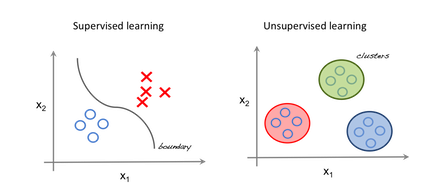
\includegraphics[scale=0.5]{./tex/induction/unsuper.png}
    \caption{Différence entre apprentissage supervisé en non supervisé}
    \label{super_unsuper}
\end{figure}


\subsubsection{Apprentissage semi-supervisé}

\noindent Une approche alternative, nommée \textit{apprentissage semi-supervisé}, propose d'exploiter des données \textbf{labellisées} et \textbf{non labellisées}. Elle est donc comparable à un mélange entre apprentissage \textit{supervisé} et \textit{non supervisé}. \\

\noindent Cette forme d'apprentissage cherche à combiner les avantages des deux approches tout en corrigeant mutuellement leurs défauts propres. L'objectif principal de cette méthode d'apprentissage est de limiter le volume de données labellisées nécessaires à l'apprentissage supervisé en reposant sur la capacité d'association des données que procure l'apprentissage non supervisé. Ainsi, à partir d'un volume restreint de données labellisées, l'algorithme sera capable d'améliorer ses règles de discrimination à partir de données non labellisées grâce aux capacités non supervisées de l'algorithme.\\

\noindent Les approches standards semi-supervisées sont l'\textit{auto-apprentissage} et le \textit{co-apprentissage}.\\

\noindent L'\textit{auto-apprentissage} cherche à apprendre un superviseur à partir d'un volume restreint de données. Le superviseur discrimine alors des données non labellisées et les prédictions à forte confiance sont ajoutées à l'ensemble d'apprentissage. Un nouveau apprentissage est alors de nouveau réalisé avec le nouveau ensemble d'apprentissage. Ce cycle peut être répété plusieurs fois.\\

\noindent Le \textit{co-apprentissage} part du postulat qu'il existe 2 (ou plus) projections indépendantes d'un même espace de données. Ainsi, il va apprendre un classifieur sur chacune de ces projections et réaliser des prédictions indépendantes. Si la prédiction des classifieurs pour une même donnée est identique\footnote{Au moins, à la majorité...}, alors la donnée est discriminée par la classe prédite.\\

\noindent Par exemple, supposons que nous voulons discriminer un individu selon son sexe. La taille, le poids et la pilosité sont des critères discriminants. Ainsi, trois projections selon ces variables permettent la création de trois classifieurs qui évalueront un individu selon ces trois critères. Dans les faits, la taille et les poids ne sont pas complètement indépendants\footnote{Le poids et la taille sont corrélés entre eux.}. Néanmoins, on peut faire l'hypothèse qu'ils le sont.

\subsubsection{Apprentissage par transfert}
\noindent L'apprentissage automatique est une tâche coûteuse en ressources et en temps. De même, elle nécessite un important volume de données. Ces contraintes sont déterminantes pour le développement et l'exploitation de l'intelligence artificielle. En effet, il peut être difficile d'avoir des données associées à une tâche précise, de même qu'il n'est pas toujours possible d'avoir à disposition, une forte capacité de calculs (ou de temps).\\

\noindent C'est dans cet environnement que l'apprentissage par transfert (\textit{Transfer Learning}) prend toute son importance. En effet, ce paradigme repose sur l'idée que les connaissances acquises lors d'un apprentissage dans un environnement particulier peuvent être utilisées pour améliorer l'apprentissage dans un autre environnement. Ainsi, il n'est plus nécessaire de supposer un contexte strictement inconnu mais au contraire, en supposer une partie déjà définie. Cette approche permet donc un gain de temps d'apprentissage et une optimisation des données considérables, ce qui est critique pour l'industrie moderne.\\

\noindent Il ne s'agit pas d'une méthode d'apprentissage à proprement parler (comme l'apprentissage supervisé ou non supervisé) mais plutôt d'une optimisation de ces dernières. Elles sont donc complémentaires. Par exemple, dans le cadre de l'apprentissage supervisé, l'apprentissage par transfert implique la possibilité de réutiliser la connaissance de la structure de dépendance entre les caractéristiques et les étiquettes apprises dans un contexte afin d'améliorer l'inférence de la structure de dépendance dans un autre contexte.\\

\noindent Supposons un phénomène particulier (ou domaine) défini sur un espace $\mathcal{X}$ par une distribution $\mathcal{P}$. Nous avons donc un domaine $\mathcal{D}$ tel que $\mathcal{D}=(\mathcal{X}, \mathcal{P})$. Nous souhaitons réaliser une tâche $\mathcal{T}$ tel que $\mathcal{T}=(\mathcal{Y},f)$ avec f, fonction-cible définie telle que $f:\mathcal{X} \rightarrow \mathcal{Y}$.\\

\noindent Supposons un cas où nous disposons de deux domaines distincts avec une tâche définie par domaine. Le premier est le domaine-source $\mathcal{D}_S$ et possède une tâche $\mathcal{T}_S$. Le second est le domaine-cible et est défini par $\mathcal{D}_C$ et $\mathcal{T}_C$. L'objectif de l'apprentissage par transfert est d'améliorer l'apprentissage de $f_{\mathcal{T}_C}$ en utilisant la connaissance issue de $\mathcal{T}_S$, $\mathcal{D}_S$ en plus de $\mathcal{D}_C$, $\mathcal{T}_C$ avec des conditions d'inégalité entre les domaines et les tâches. Par exemple, $\mathcal{D}_S \neq \mathcal{D}_C$ et $\mathcal{T}_S \neq \mathcal{T}_C$. \\

\noindent Il existe trois grandes approches d'apprentissage par transfert (voir Figure \ref{transfer_l_pic}) :
\begin{enumerate}
    \item \textbf{Transductive}: Les deux domaines sont différents\footnote{Différents mais liés par un lien quelconque permettant le transfert !} mais la tâche est la même. De plus, nous ne possédons pas de label pour les données du domaine-cible. Nous avons donc:  $\mathcal{T}_S = \mathcal{T}_C$, $\mathcal{D}_S \neq \mathcal{D}_C$ et $\mathcal{D_{C|Y}}= \emptyset$. Le cas particulier où $\mathcal{D}_S = \mathcal{D}_C$ est néanmoins possible et exploite d'autres méthodes pour être exploitées. \\

    \item \textbf{Inductive}: Les deux domaines sont identiques mais les tâches diffèrent. Nous possédons les labels pour les deux domaines ou uniquement pour le domaine cible. Nous avons donc: $\mathcal{T}_S \neq \mathcal{T}_C$, $\mathcal{D}_S = \mathcal{D}_C$\\

    \item \textbf{Non-supervisée}: Les deux domaines sont différents et les tâches diffèrent aussi. Nous ne possédons pas les labels pour les deux domaines. Nous avons donc: $\mathcal{T}_S \neq \mathcal{T}_C$, $\mathcal{D}_S = \mathcal{D}_C$ et $\mathcal{D_{S|Y}} \neq \mathcal{D_{C|Y}}=\emptyset$.\\
\end{enumerate}

\begin{figure}
    \centering
    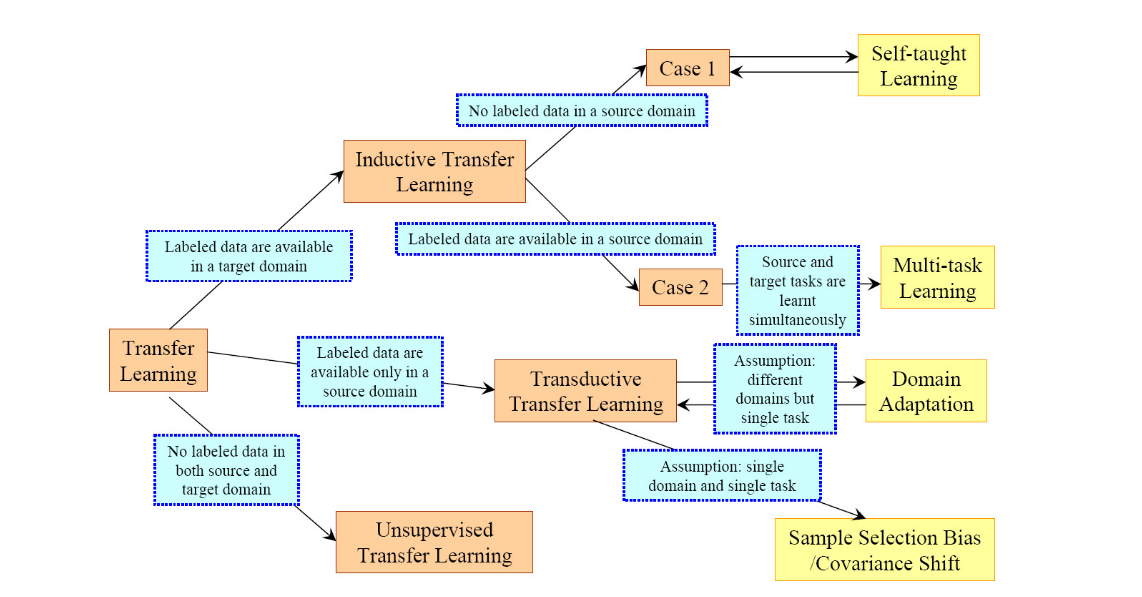
\includegraphics[scale=0.3]{./tex/induction/transfer_l.png}
    \caption{Les différentes approches d'apprentissage par transfert}
    \label{transfer_l_pic}
\end{figure}

\noindent De même, deux spécificités sont associées aux espaces des domaines. Ainsi, nous parlons d'apprentissage par transfert \textbf{homogène} si $\mathcal{X}_S=\mathcal{X}_C$. La différence se situe donc au niveau de la loi de probabilité associée à chacun des domaines. Si $\mathcal{X}_S \neq \mathcal{X}_C$, nous parlerons d'apprentissage par transfert \textbf{hétérogène}.\\

\noindent Quatre configurations de ces approches sont proposées: \textbf{Instance  Transfer}, \textbf{Feature Representation Transfer}, \textbf{Parameter Transfer} et \textbf{Relational Knowledge Transfer}\cite{transfer_l}.

\paragraph{Instance Transfer}

\noindent L'approche \textit{Instance Transfer} repose sur l'idée que des données issues du domaine source peuvent être utilisées dans un autre domaine (lié) à travers différentes méthodes de \textit{sampling} et de pondération.

\paragraph{Feature Representation Transfer}

\noindent L'approche \textit{Feature Representation Transfer} cherche à projeter la donnée issue du domaine-source dans un espace spécifique afin de faciliter la discrimination de $f_C$. Ainsi, nous définissons une fonction de projection $\phi: \mathcal{X} \rightarrow \mathcal{Z}$. De même, nous redéfinissons $h_C$ tel que $h_C=f(\phi(x);\theta_C)$.\\

\noindent Cette approche est exploitée pour modifier la donnée-source afin de faciliter l'apprentissage du modèle. Par exemple, si la donnée-source possède une dimension trop élevée, il peut être utile de la représenter à travers une dimension plus faible, ce qui permet de faciliter son apprentissage. Néanmoins, il est important de considérer la perte d'informations associée à une projection dans un autre espace.

\paragraph{Parameter Transfer}

\noindent L'approche \textit{Parameter Transfer} est utilisée lorsque la tâche-source  $\mathcal{T}_S$ et la tâche-cible $\mathcal{T}_C$ partagent des paramètres, i.e pour les hypothèses source et cible $h_S, h_C \in \mathcal{H}, \ h_S=f(x;\theta_S), \  h_C=f(x;\theta_C)$, il existe des similarités entre $\theta_S$ et $\theta_C$. Cette approche est exploitée dans le cadre du \textit{Inductive Transfer Learning}.\\

\noindent Dans le cadre du Deep Learning, il s'agit, sans doute, de la méthode la plus employée. En effet, la problématique est souvent de pouvoir réexploiter un réseau ayant appris une tâche particulière pour réaliser une autre tâche à partir d'un même phénomène. Par exemple, supposons un modèle ayant appris à discriminer des images de chats. Il est judicieux de penser qu'il peut être utilisé comme base pour apprendre à discriminer des chiens. Dans ce contexte, les deux domaines sont identiques (images quelconques définies par N pixels et prises dans un \textbf{même contexte}\footnote{Cette condition est importante car deux images de même dimension peuvent ne pas appartenir au même domaine. Par exemple, une image standardisée sur fond blanc et une image prise en conditions réelles.}) mais les 2 tâches sont distinctes car associées à la discrimination de chats ou de chiens. Pour illustrer, nous pouvons aussi citer la discrimination de texte selon un auteur donné. Les domaines sont identiques (textes dans une langue donnée\footnote{Ceci est vrai si la langue est la même car sinon, les domaines sont distincts.}) mais la tâche, différente car nous voulons discriminer des auteurs différents.

\paragraph{Relational Knowledge Transfer}

\noindent Cette approche est l'application du Transfer Learning dans le cadre de domaines où les données ne sont pas i.i.d\footnote{Cette hypothèse sur les données est au coeur de beaucoup de preuves mathématiques du Machine Learning. Dans les faits, elle est rarement vérifiée voire même complètement fausse dans le cas de données fortement dépendantes comme les graphes.} et dont la représentation à travers des \textit{relations} est possible (comme les graphes, les réseaux sociaux...). \textit{Relational Knowledge Transfer} va donc supposer que les domaines ne sont pas indépendants et i.i.d. Avec cette hypothèse, elle va donc chercher à transférer les caractéristiques relationnelles d'un domaine-source vers un domaine-cible.

\paragraph{Approches et configurations}

\noindent Plusieurs approches et configurations de Transfer Learning ont été proposées. Néanmoins, chaque configuration ne peut être employée avec chaque approche. En effet, certaines configurations nécessitent des connaissances a-priori sur le domaine-source et/ou cible qui peuvent ne pas être satisfaites. Le tableau \ref{conf_trans} récapitule les relations possibles ou non.\\

\noindent Nous pouvons observer que la configuration \textit{Feature Representation} est réalisable pour chaque approche. En effet, cette configuration nécessite que des données (labellisées ou non) indépendamment de toute autre connaissance. Cette grande tolérance la rend facilement exploitable. Au contraire de \textit{Parameter} et \textit{Relational Knowledge} qui, à travers leurs grandes dépendances aux données-sources \textbf{et} cible, sont exploitables uniquement par l'approche la plus tolérante soit l'approche \textit{Inductive}.\\

\noindent Pour approfondir les différentes problématiques du \textit{Transfer Learning}, il est vivement recommandé de consulter l'article \cite{transfer_l} qui propose un état de l'art accessible et complet.

\begin{figure}
    \centering
    \begin{tabular}{|c|c|c|c|}
        \hline
         & Inductive & Transductive & Unsupervised  \\
         \hline
         Instance &  \checkmark & \checkmark &\\
         \hline
         Feature Representation & \checkmark & \checkmark & \checkmark\\
         \hline
         Parameter & \checkmark & & \\
         \hline
         Relational Knowledge & \checkmark & &\\
         \hline
    \end{tabular}
    \caption{Configurations possibles des différentes approches de Transfer Learning}
    \label{conf_trans}
\end{figure}

\subsubsection{Apprentissage par renforcement}

\noindent L'apprentissage par renforcement est une méthode d'apprentissage qui se base sur la \textit{récompense} (positive ou négative) qu'offre l'environnement d'évolution de l'automate suite à une action réalisée par ce dernier. L'automate apprend ainsi une politique de décision (ou stratégie) afin de maximiser quantitativement ses récompenses au cours du temps. Cette apprentissage est réalisée à travers une succession d'expériences itératives qui permet à l'automate de discriminer une fonction-hypothèse de comportement (la politique) basée sur l'état courant\footnote{L'état courant correspond aux spécificités de l'automate et de l'environnement observé à l'instant considéré} et l'action à réaliser.\\

\noindent Cette méthode d'apprentissage s'approche de l'apprentissage humain basé sur \textit{l'essai}. L'automate n'a pas de repères ou d'exemples de réussite pour réaliser son apprentissage. Il apprend, par lui-même, à isoler et reproduire un comportement à suivre pour réaliser sa tâche. Ce type d'apprentissage s'affranchit ainsi de toute donnée d'apprentissage en dehors de la capacité d'évaluer la récompense issue de l'interaction avec l'environnement. Pour illustrer, nous pouvons prendre l'exemple d'un enfant qui apprend à marcher. Au début, il ne sait pas tenir debout. Il essaye une action "aléatoire" et tombe. La chute est la récompense (négative) de l'environnement. Il va donc réessayer en exploitant une autre approche. Au fil des essais, l'enfant sera capable de définir le bon comportement à suivre pour marcher. Il ne savait pas comment exploiter son corps pour réaliser cette tâche mais au fil des essais, il a pu discriminer les actions permettant de réaliser cette tâche. L'apprentissage par renforcement apprend ainsi à déterminer une méthode de décision uniquement basée sur son interaction avec l'environnement, ce qui l'émancipe de tout entité extérieure (oracle) pour orienter son apprentissage.\\

\noindent Ce type d'apprentissage est encore peu exploité par l'industrie mais constitue un milieu très actif de la Recherche. Les bases théoriques de ce type d'apprentissage sont approfondies dans la section \ref{RL_section}.

\subsection{Formalisation d'un problème d'Induction}

\noindent Un problème d'induction est défini par plusieurs composantes:
\begin{enumerate}
    \item \textbf{L'environnement}: L'environnement permet de générer des entités $x_i$ obtenues indépendamment et de manière identiquement distribuées (échantillon i.i.d) selon une distribution $D_x$ sur un espace $\mathbb{X}$. On supposera l'environnement \textbf{stationnaire} pour des raisons de simplification. Néanmoins, il est possible de considérer l'environnement comme évolutif au cours du temps. Cette particularité est souvent considérée dans le cadre de l'\textit{apprentissage en ligne}.
    \item \textbf{L'oracle}: L'oracle retourne une réponse à une entité donné (souvent un label dans le cas d'une approche supervisée) selon une distribution de probabilité $F(u_i|x_i)$ inconnues avec $u_i \in \mathbb{U}$, ensemble des réponses possibles de l'oracle.
    \item \textbf{L'apprenant}: L'apprenant applique une fonction (probabiliste ou déterministe) appartenant à un espace de fonctions $\mathbb{H}$. La sortie de l'apprenant est ainsi $y_i=h(x_i)$ avec $h \in \mathbb{H}$.
\end{enumerate}

\noindent La \textbf{tâche d'apprentissage} consiste à permettre à l'apprenant de trouver une fonction h, nommée \textbf{fonction hypothèse},  dans l'espace $\mathbb{H}$ (espaces des fonctions hypothèse possibles) permettant d'approximer (au mieux) la réponse exprimée par l'oracle. Dans le cadre de l'induction, on calcule la proximité entre la fonction hypothèse et la réponse de l'oracle à travers l'\textit{espérance de perte} sur l'ensemble des cas possibles, i.e $\mathbb{X} \times \mathbb{U}$. \\

\noindent Pour une entité $x_i$ et la réponse $u_i$ de l'oracle, on définit une \textbf{perte} $l(u_i,h(x_i))$ qui évalue le coût d'avoir prédit $h(x_i)$ lorsque la réponse était $u_i$. On définit alors le \textbf{risque réel} par:
$$R_{reel}(f) = \int_{\mathbb{X} \times \mathbb{U}}l(u_i,h(x_i))dF(x,u)$$

\noindent Il s'agit d'une mesure statistique sur l'ensemble des évènements réalisables où F(x,u) peut être une distribution de probabilité ou déterministe. La densité de probabilité de F(x,u) est inconnue. Il s'agit donc de trouver la fonction hypothèse h la plus proche de F selon la fonction de perte considérée et ce, pour les régions de l'espace $\mathbb{X}$ les plus fréquentes. On ne possède pas d'information \textit{a priori}\footnote{Se remémorer les bases de la théorie bayésienne !} sur ces régions. L'ensemble d'apprentissage est donc utilisé pour les déterminer (en mal ou en bien !). L'objectif est donc de chercher à \textbf{minimiser le risque réel inconnu} à partir d'un échantillon d'apprentissage $\mathbb{S}$ avec $\mathbb{S} \in \mathbb{X}$.\\

\noindent Le \textbf{principe inductif} permet d'expliciter ce que doit vérifier la fonction h recherchée. Pour cela, il définit la fonction de proximité décrite précédemment et se base sur l'échantillon d'apprentissage $\mathbb{S}={(x_1,u_1),...,(x_n,u_n)}$ afin de minimiser le risque réel.\\

\noindent En d'autres mots, le principe inductif formalise ce que doit vérifier la fonction hypothèse selon la fonction de perte, l'échantillon d'apprentissage et possiblement d'autres paramètres selon le principe choisi. Il s'agit d'un idéal théorique à ne pas confondre avec la méthode d'apprentissage qui correspond à une application effective du principe inductif (via un algorithme). En effet, pour un principe donné, plusieurs méthodes d'apprentissage peuvent exister. Les contraintes computationnelles ou algorithmiques sont indépendantes du principe inductif. Par exemple, dans le cadre d'une optimisation par une méthode de gradient, la méthode d'apprentissage est associée à la méthode exploitée i.e la méthode de gradient et l'optimum souhaité, l'objectif défini par le principe inductif mais cet optimum peut être obtenu par une autre approche que la méthode de gradient.

\subsection{Quelques principes d'induction}
Le principe inductif permet de définir les critères qu'une hypothèse doit respecter afin de déceler celle qui optimise la minimisation du risque réel à partir d'un ensemble fini d'exemples appelé ensemble d'apprentissage.\\

\noindent Il existe plusieurs principes inductifs et aujourd'hui encore, il s'agit d'un champ de recherche théorique important car la théorie actuelle est jugée imparfaite par le milieu scientifique\footnote{D'où la grande attention et la rigueur à avoir lors de l'utilisation de l'IA dans sa globalité.}.\\

\noindent Deux principes inductifs sont très fréquents en Machine Learning: le principe ERM et le principe de décision bayésienne. Il en existe de nombreux autres mais pour limiter d'alourdir inutilement cette partie théorique, nous les négligerons.

\subsubsection{Le principe ERM}
Le principe ERM (\textit{Empirical Risk Minimization}) repose sur l'hypothèse qu'il faut minimiser le \textbf{risque empirique}. Le risque empirique correspond à la perte moyenne (ou encore l'erreur) mesurée sur l'échantillon d'apprentissage $\mathbb{S}$. Il est défini par:
$$R_{emp}(h)=\frac{1}{n}\sum_{i=1}^nl(u_i,h(x_i))$$

\noindent Le principe ERM repose sur une hypothèse forte. Il suppose que la fonction hypothèse qui s'accorde le mieux aux données d'apprentissage est une fonction capable de correctement décrire le phénomène général observé. Elle repose sur l'axiome qu'une caractéristique observée sur les données connues est aussi vérifiées par les autres données générées par le phénomène considéré. Ainsi:
$$h_{ERM}=\underset{h \in \mathcal{H}}{ArgMin} \ R_{emp}(h)$$

\noindent Ce critère inductif est le plus populaire et exploité par l'Intelligence Artificielle moderne, notamment par le Deep Learning. Le Deep Learning cherche ainsi une fonction hypothèse qui tend à avoir un risque empirique nul\footnote{Dans les faits, atteindre cette valeur est souvent synonyme de mauvais apprentissage du fait du phénomène appelé \textit{sur-apprentissage} !}.

\subsubsection{Le principe de décision bayésienne}
\noindent Le principe de décision bayésienne repose sur une approche probabiliste, i.e choisir l'hypothèse la plus probable selon le jeu de données d'apprentissage. Comme son nom l'indique, elle exploite l'approche bayésienne.\\

\noindent L'hypothèse faite est qu'il est possible de définir une distribution de probabilité sur l'espace des fonctions hypothèses $\mathbb{H}$. La connaissance préalable du phénomène peut s'exprimer sous la forme d'une distribution \textit{a priori} de probabilités. Le jeu d'apprentissage influencera alors cette distribution initiale. Il est possible de choisir l'hypothèse la plus probable ou de définir une hypothèse composite définie par la moyenne de l'ensemble des hypothèses pondérées par leur probabilité \textit{a posteriori}\footnote{Il s'agit de la vraie approche bayésienne mais elle peut être difficile à déterminer.}.\\

\noindent Le choix de l'hypothèse la plus probable repose sur deux principes: \textit{Maximum a posteriori} (MAP) et \textit{Maximum de Vraisemblance}.\\

\noindent Si chaque erreur a une pondération équivalente, alors, la règle de décision bayésienne de risque minimal devient similaire à MAP:
$$h^*=\underset{h \in F}{ArgMax} \ p_{\mathcal{F}}(f)p_{\mathcal{X}}(x|f)$$

\noindent $p_{\mathcal{F}}(f)$ dénote la probabilité a priori que le monde soit dans l'état f, $\mathcal{F}$, ensemble des états possibles.\\

\noindent Si chaque hypothèse ont la même probabilité a priori, alors MAP est équivalent au Maximun de Vraisemblance (Maximum Likelihood) et devient:
$$h^*=\underset{h \in F}{ArgMax} \ p_{\mathcal{X}}(x|f)$$

\noindent Pour rappel, la relation liant probabilité \textit{a priori} et \textit{a posteriori} est définie par:
$$P_{a \ posteriori} = \frac{P_{vraisemblance} \times P_{a \ priori}}{P_{evidence}} \leftrightarrow P(y|x)=\frac{P(x|y) \times P(y)}{P(x)}$$
\noindent La connaissance initiale du phénomène permet de définir P(y). Les données du jeu d'apprentissage modifie le comportement \textit{a priori} à travers P(x|y). Ainsi, supposons un phénomène y rare. Il aura une probabilité \textit{a priori} faible. Cependant, si ce phénomène est très présent dans le jeu d'apprentissage alors P(y|x) sera bien plus importante d'où la nécessité de s'assurer que le jeu d'apprentissage soit représentatif du phénomène considéré. P(y) peut être initialisée de manière \textit{neutre}. Dans ce cas, seule P(x|y) sera considérée. Cette approche est utilisée lorsque aucune connaissance du phénomène est possible.\\

\noindent Dans les faits, P(x) peut être difficile à évaluer. Cependant, cette valeur est constante et ne présente pas d'intérêt car il s'agit d'un facteur constant récurrent. Il peut donc être ignoré. Il se comporte comme un facteur de normalisation, ce qui est peu utile en comparaison de la complexité de son calcul.

\subsection{Evaluation de l'apprentissage}
Dans la partie précédente, nous avons proposé deux approches pour \textit{apprendre}. Il est, cependant, fondamental de pouvoir analyser l'apprentissage et de pouvoir déterminer son comportement intrasèque. Pour cela, il est nécessaire d'exploiter des hypothèses supplémentaires liées à ce qu'on cherche évaluer du système d'apprentissage.\\

\noindent Un problème d'apprentissage est dépendant de l'environnement, de l'oracle et de la fonction de perte choisie. Lorsqu'on évalue la performance espérée d'un apprenant, il est nécessaire de déterminer le cadre liant l'environnement et l'oracle.\\

\noindent Trois cas sont possible:
\begin{enumerate}
    \item \textbf{L'analyse dans le pire des cas}: Cette approche suppose qu'on ne connaît rien \textit{a priori} sur l'environnement ni sur son comportement avec l'oracle. On cherche donc à quantifier la performance de l'apprenant dans la pire des situations. Cette approche est indépendante de l'oracle et de l'environnement (et même de la fonction-cible). Il s'agit donc d'un cadre d'étude très généraliste sans hypothèse préalable forte sur les constituantes du phénomène et de l'apprentissage. Néanmoins, les conditions identifiées seront très fortes et souvent loin de la réalité expérimentale et applicative.

    \item \textbf{L'analyse en cas moyen}: Cette approche cherche à mesurer une espérance de performance. Néanmoins, il est nécessaire de faire une hypothèse sur la distribution $D_\mathbb{X}$ (environnement) et $D_\mathbb{F}$ (fonction-cible possible). Théoriquement, cette méthode permet une mesure de performance plus fine que l'approche précédente mais dans les faits, il est difficile de l'exploiter véritablement à cause de la difficulté à estimer les probabilités \textit{a priori} et à l'obligation d'utiliser des méthodes d'approximation qui nuisent à la précision du résultat.

    \item \textbf{L'analyse dans le meilleur des cas}: Cette approche est caractérisée par l'analyse de l'apprentissage dans le meilleur des cas, i.e lorsque l'oracle et l'environnement favorisent l'apprentissage en aidant l'apprenant. Cependant, la notion d'aide est difficile à évaluer, notamment la différence entre la bienveillance (professeur) et la collusion (l'oracle devient un complice). Ce type d'analyse est aujourd'hui, peu exploitée et peu établi théoriquement parlant.
\end{enumerate}

\subsection{Théorie de l'apprentissage}

\noindent L'objectif de la \textit{Théorie de l'apprentissage} est de développer un socle théorique permettant le développement et l'analyse d'algorithmes dit d'apprentissage. Elle cherche à démontrer la faisabilité de l'apprentissage d'un \textit{concept} (aussi appelé \textit{règle de prédiction}), le volume de données nécessaire à son apprentissage et les garanties théoriques associées (borner l'erreur et la complexité). Dans un cas plus général, elle étudie aussi l'efficacité (ou non) d'algorithmes selon des conditions spécifiques.\\

\noindent \textbf{Important}: Bien que plusieurs cadres théoriques aient déjà été proposés, aucun ne fait consensus auprès du milieu scientifique. Il s'agit donc d'un domaine de recherche très actif et crucial étant donné l'engouement pour l'intelligence artificielle.\\

\subsubsection{PAC Learning (Probably Approximately Correct)}

\noindent L'une des théories principales est l'\textbf{Analyse PAC} (PAC Learning - \textit{Probably Approximately Correct})\cite{pac}.\\

\noindent L'hypothèse de PAC est de considérer que l'apprentissage d'un concept inconnu est \textit{réalisable} si il est possible d'obtenir une \textit{hypothèse} capable de l'\textbf{approximer} (Approximately) et ce, avec une \textbf{forte probabilité} (Probably).

\paragraph{Qu'est-ce qu'un problème d'apprentissage ?}

\noindent Supposons:
\begin{itemize}
    \item $\mathcal{C} \ : \ \mathcal{X} \rightarrow \mathcal{Y}$, une classe de concepts. On suppose $\mathcal{C}$ comme connu et $\mathcal{Y}$, espace discret.

    \item $h \in \mathcal{C}$, le concept cible à apprendre.

    \item $\mathcal{D}$, distribution sur $\mathcal{X}$.

    \item $S=\{(x_i,h(x_i))\}_{i=1}^m$, un ensemble d'apprentissage de dimension m tel que $x_i \in \mathcal{X}$ en accord avec la distribution $\mathcal{D}$ et i.i.d. On a $h(x_i) \in \mathcal{Y}$.

    \item $\mathcal{A}$, un algorithme d'apprentissage.

    \item $\mathcal{H}$, espace d'hypothèses apprenables par $\mathcal{A}$. On supposera $\mathcal{H}=\mathcal{C}$ dans un premier temps
\end{itemize}

\noindent Après l'observation de S, $\mathcal{A}$ choisit une hypothèse $\Hat{h} \in \mathcal{H}$ par discrimination. Un problème d'apprentissage est défini par la recherche d'une hypothèse $\Hat{h}$ avec une faible \textbf{erreur de généralisation} définie par:
$$P_{x \sim D} (\Hat{h}_S(x) \neq h(x))$$

\noindent La relation entre l'erreur de généralisation et m\footnote{La valeur de m est liée à l'erreur de généralisation car $\mathcal{S}$ est paramétré par m.}, nombre de données d'apprentissage, définit la \textit{difficulté} d'apprendre le concept h. Plus le concept est difficile, plus m sera grand avant que $\Hat{h}_S$ ait une erreur de généralisation faible.\\

\noindent \textbf{ATTENTION}:\\

\fbox{%
   \begin{minipage}{0.9\textwidth}
      Une interprétation naïve de ce problème serait de définir qu'une classe de concept $\mathcal{C}$ est \textit{apprenable} selon la définition:
\begin{itemize}
    \item $\mathcal{C}$ est apprenable si, pour tout $h \in \mathcal{C}$, $P_{x \sim D} (\Hat{h}_S(x) \neq h(x)) \leq \epsilon$ avec $m=|S|$ polynomial par $1/\epsilon$.
\end{itemize}
   \end{minipage}%
}
\\
\\

\noindent Cette définition définit une classe de concept comme apprenable si il est possible de borner l'erreur de généralisation avec un nombre \textit{raisonnable} de données d'apprentissage.\\

\noindent Bien que séduisante, cette définition \textit{déterministe} est incomplète car S est une \textbf{variable aléatoire}\footnote{Car dépendant de $x_i$ issu de $\mathcal{D}$}. De ce fait, il est nécessaire de considérer le cas où S n'est pas représentatif du concept observé.\\

\noindent Illustrons cette problématique. Supposons le jeu Pierre-Feuille-Ciseau non biaisé. Étant donné que ce jeu est un jeu de hasard et qu'il n'est pas biaisé, le concept-cible est donc associé à une fonction aléatoire qui sélectionne un des trois choix selon une probabilité 1/3.\\

\noindent Supposons que pour apprendre, notre algorithme possède des exemples de parties où $x_i$ est toujours "Feuille". De ce fait, d'après les exemples d'apprentissage, l'algorithme maximise les gains en proposant, \textit{à chaque fois}, le signe "Ciseau" (Le "Ciseau" gagne sur la "Feuille"). Or, ce choix d'hypothèse est mauvais vis-à-vis de l'erreur de généralisation. Bien que très peu probable, il est nécessaire de considérer la possibilité d'un ensemble S non représentatif issu de $\mathcal{D}$. La notion d'apprentissage PAC (\textbf{Probably Approximately Correct}) est donc proposée pour compléter cette définition.

\paragraph{Formalisation du PAC Learning}
\noindent Considérons les notations de la section précédente. Afin de formaliser le PAC Learning, il est nécessaire de définir la notion de \textit{consistence} et de \textit{sample complexity} (les termes anglophones sont conservés car les traductions françaises portent à confusion du fait de leurs multiples sens).\\

\noindent Supposons un apprenant qui produit une hypothèse $\Hat{h}_S \in \mathcal{H}$ à partir d'un ensemble d'apprentissage de taille m. Un algorithme est dit \textit{consistent} si, pour tout $\epsilon$ et $\delta$, il existe un nombre fini de données d'apprentissage m pour toute distribution $\mathcal{D}$ tel que:
$$P(P_{x \sim D} (\Hat{h}_S(x) \neq h(x)) > \epsilon) < \delta$$

\noindent Or $P_{x \sim D} (\Hat{h}_S(x) \neq h(x))=|R_{reel}(\Hat{h}_S)-R_{reel}(h)|$ d'où:
$$P(|R_{reel}(\Hat{h}_S)-R_{reel}(h)| > \epsilon) < \delta$$

\noindent En d'autres mots, un apprenant est \textit{consistent} si:
$$R_{reel}(\Hat{h}_S) \underset{m \rightarrow \infty}{\rightarrow} R_{reel}(h)$$
$$R_{emp}(\Hat{h}_S) \underset{m \rightarrow \infty}{\rightarrow} R_{emp}(h)$$

\noindent La \textit{sample complexity} est la valeur minimum de m pour qu'un algorithme \textit{consistent} respecte la condition de \textit{consistence}. Si m est fini alors $\mathcal{H}$ est dit \textit{apprenable}. Si N est une fonction polynomiale en $1/\epsilon$ et $1/\delta$, alors $\mathcal{H}$ est \textbf{PAC-apprenable}.\\

\noindent \textbf{THÉORÈME}: PAC Learning\\

\fbox{%
   \begin{minipage}{0.9\textwidth}
     \noindent Soit $\mathcal{X}$, $\mathcal{Y}$, $\mathcal{C}$,  $\mathcal{D}$ et $\mathcal{S}$. On définit $h \in \mathcal{C}$ alors un algorithme $\mathcal{A}$ est un \textbf{PAC-apprenant} pour le concept h si, sous la distribution $\mathcal{D}$ et pour tout $\epsilon,\delta \in (0,1/2)$, $\mathcal{A}$ s'exécute en temps polynomial de paramètres ($1/\epsilon,1/\delta$) et demande un volume de données d'apprentissage polynomial de paramètres ($1/\epsilon,1/\delta$) pour discriminer une hypothèse $\Hat{h}_S$ dans $\mathcal{H}$ tel que:
$$P(|R_{reel}(\Hat{h}_S)-R_{reel}(h)| \leq \epsilon) \geq 1 - \delta$$
   \end{minipage}%
}
\\
\\

\noindent Le cadre théorique du PAC Learning suppose des hypothèses fortes parfois \textit{irréelles}. En effet, la condition que $\mathcal{S}$ est un ensemble i.i.d issu de $\mathcal{D}$ peut être non atteignable. La condition i.i.d sous-entend que chaque donnée d'apprentissage est décorrélées d'une autre. Or, supposons un ensemble d'apprentissage reposant sur des extraits d'une vidéo à différents instants. Il est évident que chaque donnée extraite sera corrélée avec les précédentes et suivantes. La condition i.i.d est une hypothèse théorique au coeur du Machine Learning actuel. Bien que souvent non respectée, de nombreuses approches existent pour limiter la corrélation interne des données très préjudiciables à une bonne généralisation.\\

\noindent De même, pour qu'un algorithme soit PAC-apprenant, il est nécessaire qu'il soit \textit{efficace} sur l'ensemble des distribution $\mathcal{D}$ possibles. Ainsi, les démonstrations d'apprenant non-PAC sont souvent restreintes à la création d'une distribution peu favorable à l'algorithme étudié. Cette distribution peut être fortement improbable dans un contexte réel et de ce fait, cette condition est souvent considérée comme trop stricte. C'est pourquoi PAC Learning est une analyse dite \textbf{dans le pire des cas} car elle évalue l'algorithme selon son pire comportement possible.\\

\noindent

\paragraph{PAC Learning et espace d'hypothèses}

\noindent Dans la forme initiale du PAC Learning dite \textit{correct}, $\mathcal{H}=\mathcal{C}$. Sa forme \textit{incorrecte} assouplit cette condition en proposant $\mathcal{H} \neq \mathcal{C}$. L'ensemble des autres conditions sont respectées.\\

\noindent Cette caractéristique est utile dans le cas où un apprenant n'est pas capable d'approximer des hypothèses sur $\mathcal{C}$.

\paragraph{Agnostic PAC Learning}

\noindent Dans la version initiale du PAC Learning, nous supposons qu'il existe un concept-cible h tel que $h \in \mathcal{C}$ (et $\mathcal{C}=\mathcal{H}$). Il existe donc une hypothèse-cible qui labellise parfaitement les observations. \\

\noindent Admettons maintenant que $\mathcal{D}$ est une distribution sur $\mathcal{X} \times \mathcal{Y}$. Ainsi, $\mathcal{D}$ devient aussi une variable aléatoire selon $\mathcal{Y}$. De ce fait, les données d'apprentissage utilisés ne sont plus de la forme $(x_i,h(x_i))$ mais $(x_i,y_i)$. Il est donc possible que pour un $x_i$ donné, plusieurs $y_i$ soient possibles. En d'autres mots, l'oracle n'est plus déterministe mais probabiliste.\\

\noindent Bien que cela puisse sembler contre-intuitif, cette situation est la plus réelle. En effet, cette condition est réalisée en présence de bruits sur les données d'apprentissage, d'erreur de labellisation de l'oracle (qui peut ne pas être infaillible dans la réalité) ou encore si $h \not\in \mathcal{C}$\footnote{Une distribution sur $\mathcal{X}\times\mathcal{Y}$ ne peut etre approximée par aucune fonction sur $\mathcal{X}\rightarrow\mathcal{Y}$.} par exemple.\\

\noindent Cette situation est dit \textit{non-réalisable} car il n'existe pas de concept-cible sur $\mathcal{H}$ capable de parfaitement labelliser les données (opposée à la situation \textit{réalisable} du PAC Learning présenté initialement). l'apprenant $\mathcal{A}$ ne doit donc pas trouver une hypothèse \textit{idéale} mais une hypothèse qui minimise au mieux les erreurs. Ce cadre théorique s'appelle \textbf{Agnostic PAC Learning}\cite{agn_pac}.\\

\noindent A partir de ce postulat, nous pouvons mettre à jour la notion de risque réel qui de:
$$R(\Hat{h}_S)=P_{x\sim\mathcal{D}}[\Hat{h}_S(x)\neq h(x)]$$
\noindent Devient:
$$R(\Hat{h}_S)=P_{(x,y)\sim\mathcal{D}}[\Hat{h}_S(x)\neq y]$$

\noindent Cette écriture est une généralisation de la notion de risque réel. En effet, il est possible de définir que $\mathcal{Y}$ est une distribution déterministe qui, pour $x \in \mathcal{X}$, est égal à h(x) (il s'agit donc, dans cette situation, d'une distribution conditionnée par $\mathcal{X}$).\\

\noindent Dans le cadre \textit{agnostic}, le concept-cible peut ne pas être approximée par une fonction hypothèse sur $\mathcal{H}$. Il n'est alors possible que de discriminer une fonction hypothèse sur $\mathcal{H}$ aussi performante que la meilleure hypothèse sur $\mathcal{H}$.\\

\noindent Nous définissions la qualité de l'approximation optimale de $\mathcal{D}$ par $\mathcal{H}$ selon:
$$E(\mathcal{D},\mathcal{C})\colon=\inf_{h\in\mathcal{H}}P_{(x,y)\sim\mathcal{D}}[\Hat{h}_S(x)\neq y]$$

\noindent Une nouvelle contrainte apparaît. Dans le contexte \textit{no-agnostic}, il n'existe plus nécessairement d'hypothèse $\Hat{h} \in \mathcal{H}$ capable de parfaitement approximer les prédictions de l'oracle sur les données d'apprentissage. Il est donc nécessaire d'assouplir la condition de discrimination d'une hypothèse en considérant que l'hypothèse doit être la plus performante possible. Pour cela, nous utiliserons la notion de risque empirique tel que pour $S=\{(x_i,y_i)\}_{i=1}^m$:
$$R_{emp}(\Hat{h}_S)=\frac{1}{m}|\{i:\hat{h}_S(x_i) \neq y_i\}|$$

\noindent \textbf{THÉORÈME}: Loi forte des grands nombres\\

\fbox{%
   \begin{minipage}{0.9\textwidth}
     \noindent Soit $(X_n)_{n \in \mathbb{R}}$, suite de variables aléatoires indépendantes d'une même loi de probabilité et $Y_n=\frac{1}{n}\sum_{i=1}^n X_i$, nous avons:
$$P\left(\underset{n \rightarrow \infty}{lim} Y_n = E(X)\right) = 1$$
   \end{minipage}%
}
\\
\\

\noindent En d'autres termes, la moyenne d'une variable aléatoire (risque empirique) converge vers son espérance (risque réel) lorsque le nombre d'observations augmente.\\

\noindent Mais comment définir la condition du PAC Learning si il n'existe pas d'hypothèse parfaite ?\\

\noindent Supposons un algorithme $\mathcal{A}$ qui, pour un ensemble d'apprentissage $\mathcal{S}$ issu de $\mathcal{D}_{(\mathcal{X},\mathcal{Y})}$ propose une hypothèse $\Hat{h}_\mathcal{S} \in \mathcal{H}$ avec une erreur empirique minimale. Si il existe plusieurs hypothèse qui respecte cette condition, $\mathcal{A}$ en sélectionne une arbitrairement. Nous voulons donc, pour reprendre l'idée du PAC Learning, déterminer une borne inférieure sur m qui, pour tout $\epsilon, \delta \in (0,1/2)$, vérifie:
$$P \left(R_{reel}(\Hat{h}_\mathcal{S})-\underset{h \in \mathcal{H}}{min}R_{reel}(h) > \epsilon \right) < \delta$$

\noindent Supposons la condition suivante vraie:
$$\forall h \in \mathcal{H}, \ |R_{reel}(h)-R_{emp}(h)| \leq \frac{\epsilon}{2}$$

\noindent Alors, pour tout $h \in \mathcal{H}$:
\begin{align*}
R_{reel}(\Hat{h}_\mathcal{S}) & \leq R_{emp}(\Hat{h}_\mathcal{S}) + \frac{\epsilon}{2}\\
 & \leq R_{emp}(h) + \frac{\epsilon}{2}\\
 & \leq (R_{reel}(h) + \frac{\epsilon}{2}) + \frac{\epsilon}{2}= R_{reel}(h) + \epsilon
\end{align*}

\noindent Les inégalités précédentes sont pour tout $h \in \mathcal{H}$ et vraie d'après la \textit{Loi forte des grands nombres}. Or, nous avons une condition de minimisation de l'erreur empirique pour le choix de $\Hat{h}$. La condition est donc remplie si:
$$R_{reel}(\Hat{h}_\mathcal{S}) \leq \underset{h \in \mathcal{H}}{min}R_{reel}(h) + \epsilon$$

\noindent \textbf{THÉORÈME}: Agnostic PAC Learning\\

\fbox{%
   \begin{minipage}{0.9\textwidth}
     \noindent Soit $\mathcal{X}$, $\mathcal{Y}$, $\mathcal{C}$,  $\mathcal{D}$ et $\mathcal{S}$. On définit $h \in \mathcal{C}$ et meilleur approximation du concept-cible $c \not\in \mathcal{C}$ alors un algorithme $\mathcal{A}$ est un \textbf{agnostic PAC-apprenant} pour le concept c si, sous la distribution $\mathcal{D}$ et pour tout $\epsilon,\delta \in (0,1/2)$, $\mathcal{A}$ s'exécute en temps polynomial de paramètres ($1/\epsilon,1/\delta$) et demande un volume de données d'apprentissage polynomial de paramètres ($1/\epsilon,1/\delta$) pour discriminer une hypothèse $\Hat{h}_S$ dans $\mathcal{H}$ tel que:
$$P(R_{reel}(\Hat{h}_\mathcal{S}) \leq \underset{h \in \mathcal{H}}{min}R_{reel}(h) + \epsilon) \geq 1-\delta$$
   \end{minipage}%
}
\\
\\

\noindent Une variante dite \textit{incorrecte} de \textit{agnostic PAC Learning} est possible en autorisant la condition $\mathcal{H} \neq \mathcal{C}$.\\

\noindent De même, une variante relaxée de degrés $\alpha$ nommée \textit{$\alpha$-agnostic PAC Learning} permet d'assouplir la condition de performance en modifiant la condition telle que:
$$R_{reel}(\Hat{h}_\mathcal{S}) \leq \alpha E(\mathcal{D},\mathcal{C}) + \epsilon$$

\paragraph{Généralisation aux espaces de concepts continus}

\noindent PAC Learning est une théorie générale qui s'applique arbitrairement sur tout $\mathcal{X}$ et $\mathcal{Y}$. Néanmoins, supposons un espace de concepts $\mathcal{C}$ tel que $\mathcal{C}:\mathbb{R}^n \rightarrow \mathbb{R}$. Il s'agit donc d'un concept d'un espace discret à un espace continu.\\

\noindent Dans cette configuration, pour $h \in \mathcal{C}$, la condition de calcul de l'erreur réelle définie par:
$$R_{reel}(\Hat{h}_S)=P_{(x,y)\sim\mathcal{D}}[\Hat{h}_S(x)\neq y]$$
\noindent n'est pas efficace car trop stricte\footnote{Les conditions d'égalité sont souvent exploitées dans le cadre de problème de classification ($\mathcal{Y}$ discret) mais pas pour un problème de régression ($\mathcal{Y}$ continu).}.\\

\noindent Une généralisation du risque réel est donc nécessaire. Pour cela, nous proposons:
$$R_{reel,gen}(\Hat{h}_S)=\mathbb{E}_{(x,y)\sim\mathcal{D}}[L(\Hat{h}(x),y)]$$

\noindent L est nommée \textbf{fonction de perte}. Elle est caractérisée par $L\colon\mathcal{Y}\times\mathcal{Y}\rightarrow\mathbb{R}$. Son objectif est de mesurer la similarité entre la prédiction de l'apprenant $\mathcal{A}$ et la prédiction de l'oracle. Dans le cas d'un espace de concepts défini par un espace continu, il est commun d'exploiter la notion de \textit{distance}. Nous pouvons présenter \textit{$L_1$ Loss} définie par $L(y_{1},y_{2})=||y_{1}-y_{2}||$ ou encore \textit{$L_2$ Loss} par $L(y_{1},y_{2})=||y_{1}-y_{2}||_2^{2}$.\\

\noindent Ainsi, $R_{reel}$ est un cas particulier de $R_{reel,gen}$ tel que:
$$R_{reel}(\Hat{h}_S)=\mathbb{E}_{(x,y)\sim\mathcal{D}}[L(\Hat{h}_S(x),y)]$$
$$L(x,y)=\left\{
\begin{array}{l}
  1 \ si \ x \neq y\\
  0 \ sinon
\end{array}
\right.$$

\subsubsection{Exemple d'une étude par PAC Learning - Le principe ERM dans le cas fini}

\noindent Supposons que $|\mathcal{H}|$ est fini, i.e il existe un nombre fini d'hypothèses possibles et que la tâche est \textit{réalisable}. Ainsi il existe $\Hat{h}_S in \mathcal{H}$ telle que $R_{emp}(\Hat{h})=0$.  De même, nous utiliserons la fonction de perte L tel que:
$$L(x,y)=\left\{
\begin{array}{l}
  1 \ si \ x \neq y\\
  0 \ sinon
\end{array}
\right.$$

\begin{figure}
    \centering
    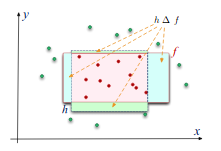
\includegraphics[scale=0.45]{./tex/induction/erm_c.png}
    \caption{Erreur entre l'hypothèse-cible et l'hypothèse apprise}
    \label{erm_c}
\end{figure}

\noindent Avec cette fonction de perte, le risque réel est égale à la probabilité qu'un exemple se situe dans la zone d'erreur entre l'hypothèse-cible et l'hypothèse apprise. En d'autres mots, il s'agit de la différence symétriques entre les deux ensembles que nous noterons $\Hat{h} \bigtriangleup h$. Une illustration de cette zone est présentée sur la Figure \ref{erm_c}.\\

\noindent Soit $\Hat{h}$ tel que $R_{reel}(\Hat{h}_S) > \epsilon$. La probabilité qu'après une observation $x \in D$, l'hypothèse apprise ne fasse pas d'erreur est donc inférieure ou égale à $1-\epsilon$.

$$P_D(\Hat{h}) = P_{(x,y) \sim D}(\Hat{h}(x)=y)$$

\noindent Supposons  m  observations:

\begin{align*}
P_D^m(\Hat{h}) &= (P_{(x,y) \sim D}(\Hat{h}(x)=y))^m\\
&\leq (1-\epsilon)^m\\
\end{align*}

\noindent Or, $1+x \leq e^x$:
$$P_D^m(\Hat{h}) \leq e^{-\epsilon m}$$

\noindent Ainsi, pour une hypothèse choisie, la probabilité de "survie est de $e^{-\epsilon m}$. Or, il est possible qu'il existe plusieurs hypothèses respectant le critère ERM mais ayant un risque réel supérieur à $\epsilon$. Ainsi, en considérant l'ensemble des hypothèses possibles $\mathcal{H}_{e}$, la probabilité qu'une hypothèse "mauvaise" soit choisie est bornée par $\sum_{h \in \mathcal{H}_\epsilon}P_D^m(\Hat{h})$

\begin{align*}
P_D^m(\forall h \in \mathcal{H}_\epsilon\Hat{h}) &= \sum_{h \in \mathcal{H}_\epsilon}P_D^m(\Hat{h})\\
&\leq |\mathcal{H}_{\epsilon}|e^{-\epsilon m}\\
&\leq |\mathcal{H}|e^{-\epsilon m}
\end{align*}

\noindent Le PAC-Learning est caractérisé par:
$$P(P_{x \sim D} (R_{reel}(\Hat{h}_S)) \leq \epsilon) > 1-\delta$$

\noindent La condition est donc respectée si:
$$m \geq \frac{1}{\epsilon}ln\frac{|\mathcal{H}|}{\delta}$$

\noindent \textbf{Important}: En réecrivant l'équation du PAC-Learning dans ce cas-ci, nous observons:
$$P(P_{x \sim D} (R_{reel}(\Hat{h}_S)) \leq \epsilon) > 1-\delta$$
$$P(P_{x \sim D} (R_{reel}(\Hat{h}_S)) \leq R_{emp}(\Hat{h})+\frac{log|\mathcal{H}|+log\frac{1}{\delta}}{m}) > 1-\delta$$

\noindent $R_{emp}(\Hat{h})=0$ par définition car nous sommes dans le cas réalisable. Nous observons donc que m est directement dépendant de $|\mathcal{H}|$ mais surtout, la borne d'erreur est directement dépendante de la cardinalité de $\mathcal{H}$. De ce fait, il est \textbf{fondamentale} de limiter l'espace des hypothèses possibles afin de favoriser l'induction. En d'autres mots, il est nécessaire de \textit{contraindre} l'espace des hypothèses avec des conditions supplémentaires. L'application de contraintes s'appelle la \textbf{Régularisation}. La \textbf{Régularisation} est très employée en Machine Learning et le Deep Learning ne fait pas exception. Elle est employée pour favoriser l'apprentissage et lutter contre le risque de sur-apprentissage.\\

\noindent \textbf{Remarque}: Cette étude de cas est relativement triviale notamment du fait qu'on a étudié le cas fini avec un espace d'hypothèse fini. Dans les cas plus généraux, l'étude de modèle est une tâche ardue et complexe qui nécessite une connaissance mathématique poussée.

\subsection{Théorie de la régularisation}
\subsubsection{Contexte et environnement}
\noindent L'induction se présente comme un problème dit \textit{mal posé}. Un problème \textit{bien posé} doit répondre à 3 critères:
\begin{itemize}
    \item \textbf{Existence}: pour toute fonction-cible h, il existe une fonction $\Hat{h} \in \mathcal{H}$ en tant que solution du problème.\\

    \item \textbf{Unicité}: $\Hat{h}$ est unique.\\

    \item \textbf{Continuité}: $\Hat{h}$ dépend \textit{continûment} de h.
\end{itemize}

\noindent Or, dans le cadre de l'induction, la condition d'unicité est souvent non respectée. De même qu'il est possible qu'il n'existe pas d'hypothèse dans $\mathcal{H}$ qui puisse parfaitement s'associer aux données, notamment si les données sont bruitées ou non représentables par l'espace $\mathcal{H}$. \\

\noindent La théorie de l'apprentissage modifie le problème \textit{mal posé} que représente le problème d'induction en ajoutant des contraintes additionnelles. Ainsi, le problème à résoudre est la recherche de $\mathcal{H}$ respectant la condition du critère inductif \textit{et} une contrainte $\Phi(\mathcal{H}) \leq \alpha$. Cette contrainte représente une caractéristique connue a priori sur la solution optimale recherchée. Elle permet de compléter la discrimination des hypothèses valides et ainsi, de diminuer le nombre d'hypothèses recevables par le modèle, i.e la cardinalité de $\mathcal{H}$.\\

\noindent Intuitivement, nous voulons supprimer les classes d'hypothèses \textit{trop} complexes, i.e capable de s'accorder à tout échantillon de dimension m. Ce type d'hypothèses est souvent associé à des hypothèses polynomiales de haute dimension. En effet, plus la dimension est élevée, plus la fonction peut expliquer une information précise du comportement observé. Or, la capacité explicative peut être telle que toute fonction de la classe peut expliquer parfaitement le comportement "grossier" issu des m exemples sans pour autant être pertinente sur l'ensemble du phénomène observé. Nous sommes donc en présence de sur-apprentissage car la fonction est trop spécialisée sur l'échantillon d'apprentissage au point de ne pas conserver une capacité de généralisation.\\

\noindent Il existe deux approches pour contraindre un espace d'hypothèses:
\begin{itemize}
    \item \textbf{Approche paramétrique}: On contraint le nombre de paramètre de l'hypothèse, i.e sa dimension. Ainsi, il est possible de limiter le nombre de connexion dans le réseau de neurones.\\

    \item \textbf{Approche non paramétrique}: Cette approche ne considère pas le nombre de paramètres mais la \textit{régularité} (smoothness) de la fonction. Ainsi, ce critère favorise les hypothèses représentées par une courbe "lisse". Une illustration est visible sur la Figure \ref{reg_no_param}. Une régularisation non paramétrique va favoriser l'hypothèse représentée par la courbe verte. Par exemple, cette régularisation limitera le degrés polynomial de l'hypothèse choisie dans le cadre d'une régression car une fonction polynomiale "lisse" tend à être une fonction polynomiale de faible degrés.
\end{itemize}

\begin{figure}
    \centering
    \includegraphics[scale=0.3]{./tex/induction/Regularization.png}
    \caption{Illustration d'une régularisation non paramétrique}
    \label{reg_no_param}
\end{figure}

\subsubsection{Définition de la régularisation}

\noindent La fonctionnelle (ou fonction) de pénalisation, que nous noterons $\Phi$, définit la connaissance a priori qui caractérise les spécificités que doivent respecter les hypothèses jugées valides par le modèle. On cherche ainsi à minimiser le \textbf{risque pénalisé}:
$$R_{reg}(h) ) R_{emp}(h) + \lambda \Phi(h)$$

\noindent $\lambda$ est un paramètre qui détermine le compromis entre la fidélité aux données d'apprentissage et les caractéristiques que doit avoir l'hypothèse. Il est difficile de connaître les caractéristiques que doit avoir l'hypothèse. Afin d'assouplir la pénalisation en cas d'informations a priori "mauvaises", le critère de pénalisation est souvent ajusté. Ainsi, on fixe la fonctionnelle mais on ajuste sa pondération selon le phénomène observé de manière empirique à partir des données d'apprentissage. En faisant varier $\lambda$, on modifie la classe d'hypothèses valorisée par le modèle. Néanmoins, comme les exemples sont issus d'un sous-ensemble de la distribution de données, les hypothèses sont nécessairement \textit{optimistes} car il est plus facile de satisfaire les conditions d'un ensemble ensemble de plus faible dimension. C'est pourquoi il est apprécié de réaliser l'apprentissage d'une fonction hypothèse pour différentes classes d'hypothèse (en faisant varier $\lambda$) et d'évaluer les différentes hypothèses sur un ensemble d'exemples indépendants de l'apprentissage (et du test). Nous parlons alors d'\textit{ensemble de validation}.

\subsubsection{Les formes de la régularisation}

\noindent Il existe trois formes principales de régularisation. Ces formes sont complémentaires et peuvent être (éventuellement) cumulées selon le cas. Ainsi, nous avons:

\begin{itemize}
    \item \textbf{Régularisation des poids}: Cette approche consiste à limiter l'importance des paramètres du modèle. En effet, un paramètre à valeur élevée favorise un sur-optimisme pour une caractéristique donnée, ce qui nuit à la capacité d'adaptation globale en sur-spécialisant l'hypothèse sur un type d'exemples non représentatif de l'ensemble du phénomène.\\

    \item \textbf{Early Stopping}: Cette approche provoque un arrêt prématuré de l'apprentissage. En effet, plus le modèle converge vers un optimum local, plus l'hypothèse devient complexe. En forçant un arrêt précoce, on limite la complexité de l'hypothèse et ainsi, le risque de perte de généralisation.\\

    \item \textbf{Échantillon bruité}: Cette approche repose sur un apprentissage à partir de données \textit{bruitées}. Les données \textit{bruitées} limite le risque que le modèle se spécialise sur l'échantillon d'apprentissage en accentuant les irégularités locales. Ainsi, l'hypothèse choisie aura tendance à favoriser les régularités dites \textit{profondes} et négligera les \textit{détails}, accentués par le bruit imposé aux données.
\end{itemize}

\subsection{No Free-lunch Theorem, un fondamental théorique (et grande désillusion ?)}

\noindent \textit{No Free Lunch Theorem}\cite{nflt} est un théorème théorique \textbf{fondamental} de l'apprentissage automatique. Ce théorème démontre une limitation forte qui modère grandement l'engouement que l'on peut avoir pour un modèle d'apprentissage ou une classe d'algorithme.\\

\noindent Supposons deux algorithmes d'apprentissage $M_1$ et $M_2$ quelconques et m, nombre de données d'apprentissage. Les propositions suivantes sont vraies:
\begin{enumerate}
    \item En moyenne uniforme sur toutes les fonctions cible f dans $\mathcal{F}$:\\
    $E_{M_1}[R_{reel}|f,m]-E_{M_2}[R_{reel}|f,m]=0$\\

    \item Pour tout échantillon d'apprentissage S, en moyenne uniforme sur toutes les fonctions cible de f dans $\mathcal{F}$:\\
    $E_{M_1}[R_{reel}|f,S]-E_{M_2}[R_{reel}|f,S]=0$\\

    \item En moyenne uniforme sur toutes les distributions possibles P(f):\\
    $E_{M_1}[R_{reel}|m]-E_{M_2}[R_{reel}|m]=0$\\

    \item Pour tout échantillon d'apprentissage S, en moyenne uniforme sur toute les distribution P(f):\\
    $E_{M_1}[R_{reel}|S]-E_{M_2}[R_{reel}|S]=0$\\
\end{enumerate}

\noindent En résumé, ces propositions démontrent \textbf{qu'aucun algorithme d'optimisation numérique n'est plus efficace qu'un autre sur l'ensemble d'un espace des problèmes}. En d'autres mots, chaque algorithme d'optimisation (aussi extraordinaire soit-il selon son créateur) est aussi performant que l'algorithme de sélection aléatoire sur l'ensemble des problématiques. Celui qui sera performant sur une classe particulière de problèmes sera mauvais sur une autre, etc... Ainsi, pas de recette miracle ! Chaque problème demandera une étude de cas poussée et un algorithme sur mesure pour le résoudre. Pour illustrer, nous pouvons voir des performances possibles et impossibles de modèles d'apprentissage sur l'ensemble des fonction-cible possible. Les signes + et - correspondent à une performance respectivement supérieure et inférieure à la sélection aléatoire. 0 indique une performance équivalente au hasard.\\

\begin{figure}
    \centering
    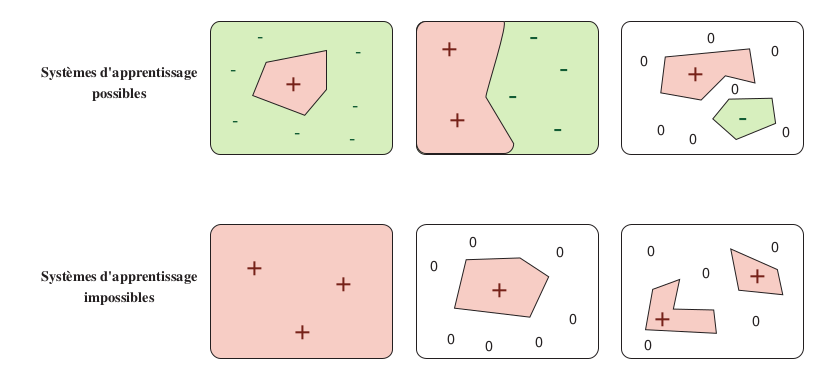
\includegraphics[scale=0.3]{./tex/induction/no_free.png}
    \caption{La fin du rêve: No Free Lunch Theorem}
    \label{no_free}
\end{figure}
\noindent Pour être capable de discriminer, un modèle repose sur des hypothèses. Ces hypothèses sont des \textbf{biais prédictifs}. Sans biais, impossible d'apprendre. Néanmoins, ces hypothèses peuvent être contre-productives pour un contexte donné et utiles dans d'autres. Il est donc nécessaire de faire des hypothèses au cas-par-cas, ce qui met fin au rêve d'un modèle parfait supérieur à tous !\\

\noindent \textbf{Remarque}: Cette restriction est néanmoins nuancée. En effet, parmi l'ensemble des problématiques de l'espace des problèmes, nombreuses sont celles qui ne correspondent pas à un phénomène réel pertinent ou "naturellement réalisable". De ce fait, il est possible de voir un modèle considéré comme "supérieur" du fait de sa grande performance sur des problématiques répandues dans notre société actuelle. Il ne faut pas oublier que cet avantage se paie dans une partie de l'espace, certes, non pertinente mais bien réelle. \\

\noindent De même, ce théorème s'applique à un modèle précis et non une classe de modèle. Dans une même classe, il existe une multitude d'architectures plus ou moins performantes selon la problématique. Dans le cadre du Deep Learning, les architectures sont particulièrement diversifiées, ce qui permet au Deep Learning d'être performant dans l'ensemble des problématiques actuelles du fait de cette richesse d'architecture. Mais il est fondamental de retenir qu'un modèle neuronal spécifique n'est pas supérieur à un autre, qu'une classe d'architecture neuronale n'est pas supérieure à une autre mais surtout, \textbf{le Deep Learning n'est pas plus performant que les architectures de Machine Learning classiques} (quoi qu'il puisse être vu, lu ou entendu...) !

\newpage

%% Fondamentaux.
\section{Les Fondamentaux}


\subsection{Deep Learning, le fer de lance du Machine Learning}
Le deep Learning est une catégorie d'algorithmes basée sur un assemblage spécifique d'entités nommées \textbf{neurones}\footnote{Une analogie peut être réalisée avec le cerveau humain}. Ces entités sont assemblées sous forme de couches plus ou moins nombreuses et profondes, à l'architecture variable selon la complexité du modèle recherché et du problème à résoudre.\\

\noindent Le Deep Learning modélise les données avec une haute capacité d'abstraction où chaque couche extrait et transforme les données issues de la couche précédente\footnote{Selon le type d'architecture, il peut y avoir des phénomènes de rétro-action} avec une approche majoritairement \textbf{non linéaire}. Un réseau possède donc un niveau d'abstraction dépendant de son architecture. Ainsi, les couches les plus basses discrimineront des phénomènes simples et généralistes\footnote{Non spécifiques au phénomène observé.} alors que les couches supérieures discrimineront des phénomènes plus complexes et caractéristiques du phénomène observé. La Figure \ref{absdl} illustre un exemple d'analyse d'une image. Nous pouvons observer que la première couche discrimine des structures géométriques simples telles que des lignes ou des courbes alors que les couches suivantes discriminent des structures plus complexes. Il n'y a pas de méthodologie reconnue pour déterminer l'architecture \textit{idéale} pour une problématique donnée. Seule l'approche empirique est employée à ce jour.\\

\begin{figure}
    \centering
    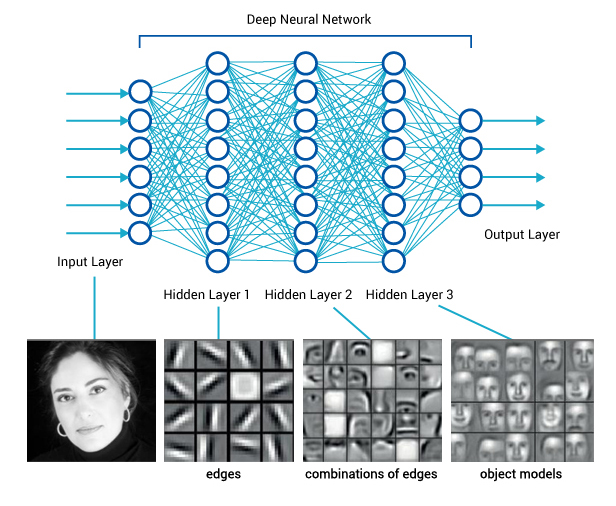
\includegraphics[scale=0.45]{./tex/fondamentaux/dlabs.jpg}
    \caption{Relation entre profondeur du réseau et capacité d'abstraction}
    \label{absdl}
\end{figure}

\noindent Aujourd'hui, le Deep Learning est très populaire pour ses résultats qui sont, dans de nombreux domaines, les meilleurs de l'état de l'art. Néanmoins, sa grande qualité repose sur sa capacité à s'émanciper du travail de pré-traitement des données nécessaires aux méthodes plus classiques. Par exemple, une image, pour être exploitée par des modèles standards, doit être pré-traitée pour extraire son contenu utile. Ces méthodes d'extraction sont généralistes, lourdes à employer et pas toujours efficaces. Les modèles de Deep Learning (notamment convolutifs\footnote{Nous l'étudierons dans cette introduction}) ont la capacité d'apprendre dynamiquement l'extraction du contenu utile d'une image. Ainsi, le réseau se spécialise - sans intervention humaine - sur le type d'image qu'il traite et bien souvent, dépasse les performances de méthodes de pré-traitement standards. Cette capacité d'auto-apprentissage rend le Deep Learning modulable, simple\footnote{La simplicité est relative...} et facilement déployable. En effet, en simplifiant, il suffit de donner la donnée brute et le réseau s'adaptera seul. Cette capacité se généralise à différents types de données: signal 1D (texte, signal sonore), signal 2D (image), séries temporelles... Cependant, il est nécessaire d'adapter l'architecture du modèle au type de données et au problème ciblé.\\

\noindent Cette souplesse d'utilisation a un coût non négligeable: \textbf{le volume de données}. Pour être fonctionnel, un réseau de Deep Learning doit exploiter un volume très important de données durant son apprentissage\footnote{Le volume dépend de la tâche à accomplir et de la nature des données}. Aujourd'hui, peu d'acteurs du milieu public ou privé ont un volume suffisant à disposition. Le Deep Learning ne constitue donc pas un remplaçant absolu aux approches de Machine Learning traditionnelles mais une alternative lorsque l'apprentissage peut être réalisé dans de bonnes conditions. De même, les architectures de Deep Learning sont exigeantes en temps machine et en ressources. Il est parfois pertinent d'exploiter des modèles plus légers et accessibles lorsque la tâches à accomplir ne nécessite pas un modèle à forte complexité.\\

\noindent De ce fait, aujourd'hui, pour les tâches d'\textit{optimisation}, le Machine Learning traditionnel garde une place dominante alors que sur des thématiques complexes ou créatives (génération automatique, traduction...), le Deep Learning devient nécessaire.\\

\noindent \textbf{Important}: Le Deep Learning profite d'une médiatisation importante qui tend à extrapoler ses qualités. Il est crucial de comprendre en profondeur les qualités et les défauts de ce type de modèle afin de ne pas alimenter les risques d'un développement non maîtrisé et biaisé.

\subsection{Un neurone: le perceptron}
Le modèle le plus simple correspond au modèle unitaire: un seul neurone. Ce modèle est appelé \textbf{perceptron} et a été inventé en 1957 par Frank Rosenblatt. La Figure \ref{perceptron} représente un neurone.\\

\noindent Le perceptron (neurone) \textbf{selon Rosenblatt} est défini par différents éléments. Ainsi, un neurone j est décrit par:\\
\begin{itemize}
    \item Des données d'entrée: $x_1,x_2,...,x_n$
    \item Des poids (qui pondèrent les données d'entrée): $\omega_1,...,\omega_n$
    \item Un biais (qui régule l'activation du neurone): $b_j$
    \item Une fonction d'activation (qui modélise la réponse du neurone en fonction des entrées pondérées): $\varphi()$ avec $\varphi= \left\{\begin{array}{ll}0 \ si \ x<0 \\1 \ si \ x> 0\end{array}\right.$ (fonction heavyside\footnote{Nous verrons par la suite que c'est un très mauvais choix de fonction !})
    \item Une réponse (ou sortie): $y_j$
\end{itemize}

\begin{figure}
    \centering
    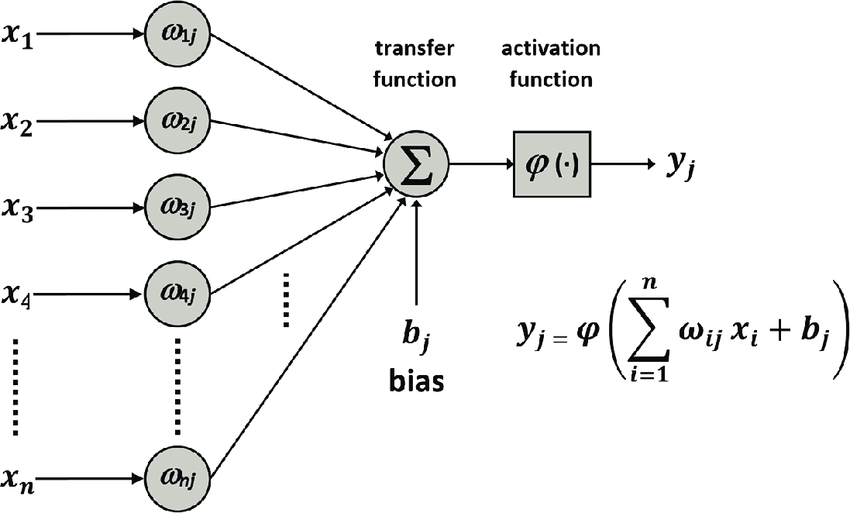
\includegraphics[scale=0.3]{./tex/fondamentaux/perceptron.png}
    \caption{La structure d'un neurone (perceptron)}
    \label{perceptron}
\end{figure}

\noindent Le fonctionnement d'un neurone est simple. \\
Supposons une entrée $[x_1,...,x_n]$ (de dimension n). Chaque entrée i est pondérée par un poids $\omega_i$ associé\footnote{il y a donc n poids}. Ainsi:
$[x_1,...,x_n]\underset{\omega}{\longrightarrow}[x_1*w_1,..,x_n*w_n]$\\

\noindent Une somme est réalisée de l'ensemble des données d'entrée pondérées et le biais $b_j$. On obtient donc: $transfer\_function=\sum_{i=1}^n (x_i*w_i)+b_j$\\
Le biais est souvent représenté comme une valeur d'entrée constante (supposons 1 par exemple) et pondérée par un poids comme le serait une autre entrée. Ainsi, nous obtenons: $transfer\_function=\sum_{i=1}^n (x_i*w_i) + w_0=\sum_{i=0}^n (x_i*w_i)$ avec $x_0=1$\\

\noindent La somme obtenue est transformée par une fonction d'activation $\varphi()$ et définira la sortie $y$ du neurone: $y=\varphi(transfer\_function)$

\subsection{Le biais}
Le biais est utilisé pour éviter que l'hyperplan réalisé par le neurone ait l'obligation de passer par l'origine. L'impact, la détermination et la représentation du biais sont encore un sujet d'étude et de recherche. Afin de ne pas complexifier cette introduction avec des approches mathématiques \textit{secondaires}, nous n'approfondirons pas cette problématique. Cependant, il est important d'avoir une sensibilité sur son utilité. Un exemple simple permet de la comprendre.\\

\noindent Supposons une image complètement noire (pixels à 0) et une sortie souhaitée égale à $\lambda$. Cette problématique est insoluble car, avec les fonctions d'activation standards, la valeur de sortie par rapport à une stimulation nulle est invariable et correspond à la valeur de la fonction d'activation en 0. Supposons la fonction heavyside, la sortie serait donc de 0.5 et constante.\\

\noindent Néanmoins, dans le cadre d'un réseau profond, le biais tend à voir son impact diminuer avec la complexité du modèle où le comportement d'activation est partiellement réalisé par des neurones de la couche précédente. Ainsi, dans le contexte du deep learning où les modèles se complexifient énormément, la gestion du biais peut être simplifiée voir "délaissée".\\

\noindent Dans les réseaux profonds, le biais est aussi utilisé pour se protéger des défauts liées à l'initialisation des neurones, notamment le phénomène \textit{Dead ReLu}\footnote{Voir Section \ref{relu_danger}, partie fonction d'activation, ReLu}.

\subsection{Le Perceptron Multicouche}

Un neurone unique possède des qualités limitées\footnote{Par exemple, il ne peut traiter que des problèmes linéairement séparables} et ne peut résoudre que des problèmes simples\footnote{Ils sont souvent employés pour simuler des portes logiques par exemple}. Afin de résoudre des problèmes plus complexes, il est nécessaire d'en assembler plusieurs afin de créer une architecture plus performante. La première architecture que nous verrons est le modèle \textit{FeedForward}.\\

\noindent Le modèle FeedForward est caractérisé par des couches de neurones où chaque neurone est connecté à l'intégralité des neurones de la couche suivante, permettant une \textit{propagation en avant} de l'information. Le réseau le plus populaire se reposant sur ce modèle est le Perceptron Multicouche. La Figure \ref{multicouche} en présente un exemple.\\

\begin{figure}
    \centering
    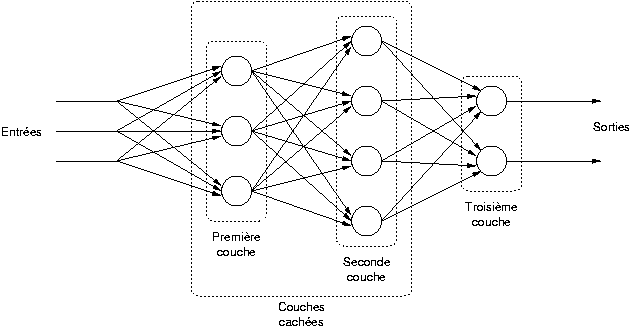
\includegraphics[scale=0.4]{./tex/fondamentaux/multicouche.png}
    \caption{Modèle FeedForward: Le Perceptron multicouche}
    \label{multicouche}
\end{figure}

\noindent Ainsi, les données d'entrées sont réparties sur la couche d'entrée composée de 1 ou plusieurs neurones où chaque donnée est envoyée à l'intégralité des neurones. Les sorties de ces neurones sont connectées à l'intégralité des neurones de la couche suivante, appelée couche cachée. Il peut y avoir plusieurs couches cachées. Les données d'entrées des couches cachées sont donc les sorties des neurones de la couche précédente. La couche de sortie correspond à la dernière couche du réseau et la sortie des neurones de cette couche correspond à la prédiction réalisée par le réseau. Ainsi, par exemple, dans un problème de classification à N classes\footnote{Voir Section \ref{multiclasslabel} pour plus de détails}, la couche de sortie sera composée de N neurones où les N sorties correspondent à la prédiction associée à chacune des classes (souvent sous forme probabiliste).\\

\noindent Le nombre de neurones par couche et le nombre de couche nécessaire pour résoudre un problème ne peuvent être déterminés à l'avance. Il n'existe pas de méthode reconnue pour obtenir le réseau "idéal" pour résoudre un problème. Néanmoins, plus le nombre de neurones et/ou de couches est élevé, plus le modèle possède un haut pouvoir d'abstraction. Avoir une haute capacité d'abstraction est nécessaire sur des problématiques complexes mais augmenter la taille du réseau ne garantit pas un meilleur résultat sur l'ensemble des problèmes et présente des risques non négligeables que nous approfondirons dans la suite de cette introduction.\\

\noindent En théorie, un perceptron multicouche à une couche cachée est capable d'approximer toute fonction d'un sous-ensemble compact de $R^n$ avec un nombre fini de neurones\footnote{Malheureusement, la méthode d'apprentissage à base de descente de gradient limite grandement les capacités d'apprentissage d'un réseau. Il n'existe pas d'alternative significativement meilleure actuellement.}. Il est donc considéré comme un \textbf{approximateur universel} de fonctions. Ce résultat est théorique et ne considère pas les difficultés d’apprentissage et de stabilité pour des problèmes complexes en très grande dimension caractéristique du Deep Learning.

\subsection{L'apprentissage du neurone}

\noindent Un neurone est défini par ses poids (et son biais). Lors de la création du neurone, les poids sont générés arbitrairement. Il est donc nécessaire de lui permettre \textit{d'apprendre}, i.e mettre à jour ses poids, afin qu'il puisse limiter ses erreurs de prédiction, i.e minimiser la valeur de la fonction de coût. Cet objectif est réalisé en deux étapes: l'étape \textit{Forward} et l'étape \textit{Backward}.\\

\noindent L'étape \textit{Forward} consiste à déterminer une prédiction réalisée par le neurone et à calculer l'erreur (potentiellement cumulée) réalisée par rapport à une valeur de référence indiquée par les données d'apprentissage. L'étape \textit{Backward} réalise la mise à jour des poids du neurone en fonction de l'erreur réalisée  grâce à l'algorithme de \textbf{Rétropropagation du gradient}.

\subsubsection{Etape Forward: Fonction de coût}
\label{fn_cout}
\noindent Afin de pouvoir mettre à jour les poids, il est nécessaire de savoir lorsque le neurone s'est trompé et quelle est l'ampleur de son erreur. La fonction de coût est utilisée pour quantifier cette erreur. Il existe différentes fonctions de coût selon la problématique à traiter. Les principales sont définies par:\\

\noindent Soit $\hat{y}$, prédition du neurone, y, valeur de référence de la donnée d'apprentissage et n, nombre de prédictions faites:
\begin{itemize}
    \item Problème de \textbf{régression}:
    \begin{itemize}
        \item \textbf{Mean Squared Error}: $\boldsymbol{\mathcal{L}}=\frac{1}{n}\sum_{i=1}^{n}(y^{(i)}-\hat{y}^{(i)})^{2}=\frac{1}{n}\sum_{i=1}^{n}(\| \hat(y) - y \|_2)$\\

        Cette fonction est la fonction la plus répandue et standard. Sa forme quadratique justifie qu'elle est convexe et ainsi, favorise l'apprentissage du réseau de neurone qui s'apparente à un problème d'optimisation. Cette fonction, du fait de la mise au carré, maximise l'importance des \textit{grandes erreurs}. C'est une spécificité importante à considérer car elle rendra l'apprentissage sensible aux valeurs extrêmes. De plus, cette fonction favorise une vitesse de convergence relativement lente du réseau de neurone.\\

        \item \textbf{ Mean Squared Logarithmic Error}: $\boldsymbol{\mathcal{L}}=\frac{1}{n}\sum_{i=1}^{n}\big(\log(y^{(i)}+1)-\log(\hat{y}^{(i)}+1)\big)^{2}$\\

        Cette fonction est une variante de Mean Squared Error à la différence qu'elle est moins sensible aux \textit{grandes erreurs} de prédiction. Dans le cas de données non normalisées aux échelles différentes, cette fonction limite la pénalisation des grands écarts de prédiction qui peuvent être liés, dans ce contexte, à l'échelle des données et non une véritable erreur de prédiction.\\

        \item \textbf{Mean Absolute Error}: $\boldsymbol{\mathcal{L}} = \frac{1}{n}\sum_{i=1}^{n}(|  \hat(y)_i - y_i |) = \frac{1}{n}\sum_{i=1}^{n}(\| \hat(y) - y \|_1)$\\

        Alors que \textit{Mean Squared Error} est empiriquement plus précise et performante dans le cadre d'une optimisation, \textit{Mean Absolute Error} produit des solutions plus \textit{éparses}\footnote{Isole les attributs fortement discriminants en minorant les attributs faiblement informatifs}, ce qui est utile dans le cadre d'extraction d'attribut pour les problèmes à haute dimension. De même, cette fonction de perte est plus résistante aux valeurs aberrantes (\textit{outliers}) et ignore les détails spécifiques, ce qui peut être utile pour lutter contre le sur-apprentissage. Néanmoins, cet aspect est responsable d'une perte d'informations, ce qui tend à la rendre empiriquement moins performante que son homologue basé sur la distance $L_2$ bien que plus stable. \\

        Dans les faits, cette fonction n'est pas dérivable en 0, ce qui est problématique dans le cadre de la rétropropagation du gradient\footnote{Cet aspect sera détaillé par la suite.}. Pour corriger ce défaut, une variante a été proposé nommée \textit{Smooth $L_1$}:
        $$| d |_{\text{smooth}} =   \begin{cases}
          0.5 d^2, & \text{if}\ | d  | \leq 1 \\
          | d | - 0.5, & \text{otherwise}
        \end{cases}$$
    \end{itemize}
    \item Problème de \textbf{classification}:
    \begin{itemize}
        \item \textbf{Cross Entropy}: $\boldsymbol{\mathcal{L}}=-\frac{1}{n}\sum_{i=1}^{n}\big[y^{(i)}\log(\hat{y}^{(i)})+(1-y^{(i)})\log(1-\hat{y}^{(i)})\big]$\\

        Cette fonction est la fonction standard dans le cadre de la classification binaire. Contrairement aux fonctions quadratiques, elle possède une vitesse de convergence plus rapide et tend à favoriser la convergence vers le minimum global (mais rien ne garantit cela !)\\

        \item \textbf{Negative Logarithmic Likelihood}: $\boldsymbol{\mathcal{L}}=-\frac{1}{n}\sum_{i=1}^{n}\log(\hat{y}^{(i)})$\\

        Cette fonction de coût est employée dans le cadre de problème de classification multi-classe. Elle peut être considérée comme une généralisation de la Cross Entropy.

    \end{itemize}
\end{itemize}

\noindent Il existe de nombreuses autres fonctions de coût aux spécificités particulières. Le choix de la fonction de coût demande de l'intuition et une certaine sensibilité mathématique. Cependant, son choix est crucial pour un fonctionnement optimal du réseau de neurones. Le travail d'analyse des différentes fonctions est un étape indispensable pour l'étude de problèmes complexes.\\

\subsubsection{Etape Backward: Rétropropagation du gradient}
\label{backward}

La fonction de coût détermine l'erreur du neurone durant son apprentissage. L'étape suivante est de permettre au neurone d'apprendre, d'évoluer en fonction de l'erreur réalisée et de faire varier chaque poids selon son impact dans l'erreur produite. Pour cela, la \textit{descente de gradient}\footnote{Il s'agit d'une méthode d'optimisation simple mais efficace. Il est possible d'en exploiter d'autres mais à ce jour, cette approche fait consensus dans la communauté scientifique.} est utilisée \textit{localement} et son application récursive sur les différents neurones du réseau forme l'algorithme de \textbf{Rétropropagation du gradient}. \\

\noindent La descente du gradient est un algorithme d'optimisation exploitée dans le cadre de la minimisation (ou de la maximisation) d'une fonction objectif f(x) paramétrée par x. Dans le cadre du \textit{Machine Learning}, nous chercherons à minimiser la fonction objectif, i.e diminuer l'erreur d'apprentissage. La fonction objectif est de dimension $R^d$ où d, nombre de paramètres du modèle.\\

\paragraph{Les méthodes de descente}
La méthode de \textit{Descente du gradient} est une méthode de descente. Avant d'expliquer les spécificités de la descente du gradient, il est nécessaire d'expliciter la notion de méthode de descente.\\

\noindent A partir d'un point $x_0$, une méthode de descente va générer une suite $(x_k)_{k \in \mathbb{N}}$ telle que:
$$x_{k+1}=x_k+\alpha_kd_k$$
$$\forall k \in \mathbb{N}, f(x_{k+1})\leq f(x_k)$$

\noindent Deux paramètres sont donc à déterminer: la direction de descente $d_k$ et la valeur du pas $\alpha_k$. La méthode de détermination de la direction de descente est utilisée pour nommer l'algorithme. La recherche de la valeur du pas est nommée \textit{recherche linéaire}.\\

\noindent \textbf{Important}: Cette partie a pour vocation d'introduire le concept d'optimisation differentiable nécessaire pour comprendre l'algorithme de Rétropropagation du gradient. De ce fait, elle est très restreinte et incomplète pour une compréhension approfondie. La section \ref{optimizer} approfondit spécifiquement les spécificités de ces algorithmes dans le cadre du Deep Learning, notamment le \textbf{calcul du pas} et les particularités liées au jeu d'apprentissage.

\paragraph{La direction de descente}
Soit une fonction objectif $f \in \mathbb{R}^n$. Une direction de descente est définie par un vecteur $d \in \mathbb{R}^n$ si pour un point $x \in \mathbb{R}^n$, $t \rightarrow f(x+td)$ est décroissante pour $t=0$. En d'autres mots, s'il existe $\epsilon > 0$ tel que:
\begin{equation}
\forall t \in ]0,\epsilon], f(x+td)<f(x)
\label{eq_direc_des}
\end{equation}
\noindent Dans le cadre classique des méthodes de descente, la fonction à minimiser est \textit{differentiable}\footnote{Dans les faits, nous souhaitons qu'elle soit une fois ou deux fois differentiable selon la méthode de descente choisie.}. De ce fait, nous pouvons dire que d est une direction de descente de f en $x \in \mathbb{R}$ ssi:
$$f'(x;d) = f'(x).d = \langle \nabla f(x),d \rangle = \nabla f(x)^Td < 0$$
\noindent Ceci garantie une décroissance de la fonction f selon la direction de d car:
$$ \forall \beta < 1, \exists \epsilon > 0, \forall t \in [0,\epsilon], f(x+td)<f(x)+t\beta \nabla f(x)^Td<f(x)$$

\paragraph{Algorithme des méthodes à direction de descente}
L'objectif de cet algorithme est de déterminer $\underset{x \in \mathbb{R}^n}{min}f(x)$.\\

\noindent Supposons $f:\mathbb{R}^n \rightarrow \mathbb{R}$ differentiable\footnote{De degrés nécessaire selon les méthodes internes choisies} et $|\epsilon| \in [0,\nu]$ avec $\nu$, petit. Au début de l'itération k, nous disposons de $x_k \in \mathbb{R}^n$. Ainsi:

\begin{enumerate}
    \item \textit{Critère d'arrêt}: si $\nabla f(x_k) \leq \epsilon$, arrêt de l'algorithme
    \item Sélection d'une direction de descente $d_k \in \{ d \in \mathbb{R}^n : \langle \nabla f(x),d \rangle < 0\}$
    \item \textit{Recherche linéaire}: calcul du pas $\alpha_k$ selon une approche spécifique
    \item $x_{k+1}=x_k+\alpha_kd_k$
\end{enumerate}

\noindent Tant que le critère d'arrêt n'est pas atteint, l'algorithme continue à  itérer. Il s'agit donc d'une famille d'algorithme \textbf{itératif}.

\paragraph{Détermination de la direction de descente}
L'une des difficultés de cette classe d'algorithme d'optimisation est la détermination de la direction de descente. C'est un sujet de recherche toujours actif. Dans le cadre de cette section, nous nous limiterons à l'étude des méthodes de descente en optimisation différentiable sans contrainte.\\

\noindent Aujourd'hui, deux stratégies sont exploitées:
\begin{itemize}
    \item \textbf{L'approche de Cauchy}: L'approche de Cauchy repose sur l'exploitation du gradient, i.e:
    $$d_k=-\nabla f(x_k)$$

    Elle est à l'origine des méthodes dites \textit{algorithmes du gradient} (ou de la plus profonde descente). Cette approche est la \textbf{référence} dans le cadre des algorithmes de Deep Learning car les algorithmes associés sont de faible complexité algorithmique et de ce fait, véloces. Néanmoins, ses performances théoriques sont limitées bien qu'empiriquement satisfaisantes. Pour pouvoir exploiter cette approche, la fonction à optimiser doit être \textbf{au moins} une fois différentiable.

    Le pas optimal $t_k$ est défini par:
    $$\nabla f(x_k+t_kd_k)=0$$

    En d'autres mots, l'algorithme converge vers un \textit{point stationnaire}, plus spécifiquement un \textbf{minimum local}. Le fait qu'il soit local est une caractéristique très importante car à l'origine d'une faiblesse théorique de performances.

    \item \textbf{Approche du gradient conjugué}:
    L'algorithme du gradient conjugué est une variante des algorithmes du gradient. L'idée est de construire itérativement des directions $\underset{k \in [0,n]}{d_k}$ mutuellement \textit{conjuguées}. Ainsi, chaque direction $d_k$ est obtenue par combinaison linéaire du gradient en $x_k$ et de la direction précédente $d_{k-1}$, elle-même dépendante de $d_{k-2}$ etc... Ainsi, nous avons:
    $$
        d_k = \left\{
            \begin{array}{ll}
                -\nabla f(x_k) & \mbox{si } k=0 \\
                -\nabla f(x_k) + \beta_kd_{k-1} & \mbox{si } k > 0
            \end{array}
        \right.
    $$

    Cette approche a inspiré les méthodes dites \textit{de moment} dans le cadre des optimizers\footnote{La tion d'optimizer sera détaillée en détail dans la suite de cette introduction} utilisés pour le Deep Learning.

    \item \textbf{Stratégie de Newton}: L'approche de Newton repose sur l'exploitation du hessien, i.e $$d_k=-H[f](x_k)^{-1}\nabla f(x_k)=-\nabla^2f(x_k)^{-1}\nabla f(x_k)$$

    Elle est à l'origine des méthodes dites \textit{algorithmes de Newton}. Comparée à l'approche par gradient, cette stratégie est bien plus performante et théoriquement robuste. Néanmoins, calculer le hessien, dans le cadre du Deep Learning, est techniquement irréalisable. En effet, l'algorithme est de complexité $O(n^3)$, ce qui le rend trop gourmand en capacités computationnelles\footnote{Cette méthode pose aussi problème au niveau du coût mémoire nécessaire à stocker le hession. La matrice hessienne est de dimension n*n pour une fonction à optimiser sur $\mathbb{R}^n$, ce qui peut être très lourd dans le cadre d'un modèle neuronal très profond avec des millions de paramètres.}. Du fait de l'utilisation du hessien, la fonction à optimiser doit être \textbf{au moins} deux fois différentiable et le hessien, inversible.

    Bien que non fonctionnelle en l'état, cette approche a inspiré des alternatives dans le cadre du Deep Learning. C'est notamment le cas de l'optimizer \textit{Adadelta}.
\end{itemize}

\noindent Il existe de nombreuses autres stratégies. Nous ne les approfondirons pas car les méthodes du gradient sont les seules véritablement exploitées dans le cadre du Deep Learning\footnote{Bien que la recherche soit activée sur l'utilisation d'approches plus performantes.}.\\

\noindent Le Figure \ref{graddes} illustre le comportement d'une optimisation par descente de gradient. La descente de gradient ne garantit pas de trouver le minimum \textbf{global} ! Cette particularité est très importante car cela signifie qu'un modèle neuronal ne converge pas vers un état idéal mais uniquement vers la meilleure tendance locale ! Deux modèles ayant appris sur des mêmes données peuvent donc être différents. Ceci est très problématique et responsable d'une faiblesse théorique de ce type de modèle et plus globalement, du Machine Learning actuel.

\begin{figure}
    \centering
    \begin{tabular}{cc}
        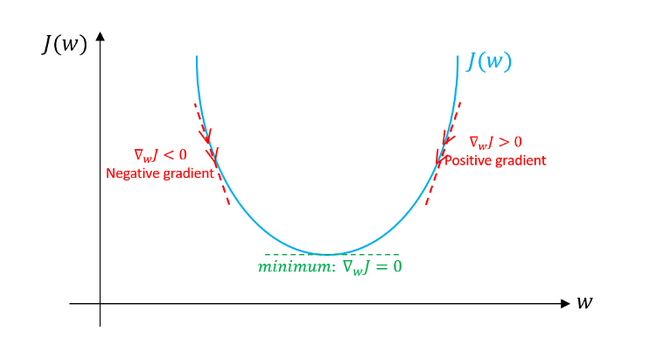
\includegraphics[scale=0.35]{./tex/fondamentaux/graddes.png} &  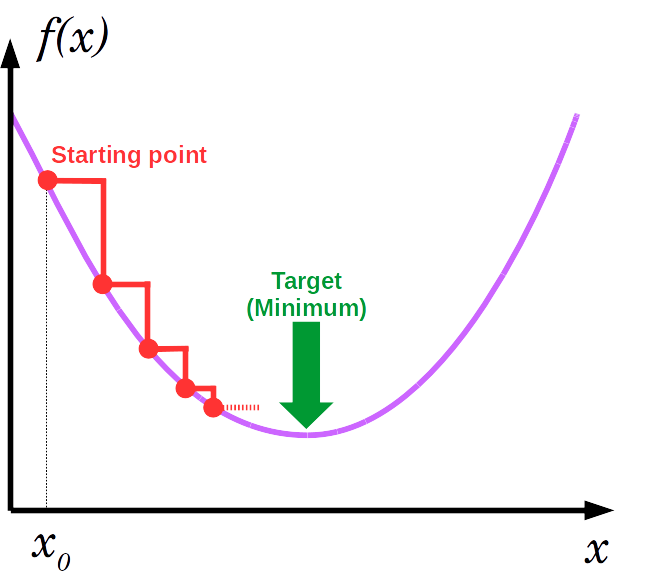
\includegraphics[scale=0.3]{./tex/fondamentaux/graddes2.png}
    \end{tabular}
    \caption{Illustration de la descente de gradient}
    \label{graddes}
\end{figure}

\paragraph{Rétropropagation du gradient - A FAIRE}


\paragraph{Fonction d'activation}

\noindent Bien que le perceptron de Rosenblatt utilise la fonction Heavyside comme fonction d'activation, il est possible d'en utiliser d'autres. Comme pour le choix de la fonction de coût, le choix de la fonction d'activation est capitale dans le développement d'un réseau de neurones. Il n'y a pas de méthodes clairement définies dans le choix de cette fonction. Les méthodes sont exclusivement empiriques bien que certaines fonctions semblent "sortir du lot"\cite{loss_deep}. \\

\noindent Pour être pleinement fonctionnelle, les fonctions d'activations doivent présenter des caractéristiques particulières dépendantes des spécificités de l'algorithme de \textit{Rétropropagation du gradient}:
\begin{itemize}
    \item \textbf{Être dérivable en tout point}: Le gradient étant dépendant de la dérivée de la fonction d'activation, une fonction non dérivable est difficilement utilisable.
    \item \textbf{La dérivé doit être non nulle}: Si la dérivée de la fonction d'activation est nulle, le gradient sera nul. De ce fait, l'apprentissage est impossible. Ce problème justifie la non-efficacité de la fonction Heavyside du perceptron standard car il \textbf{ne peut pas apprendre} en faisant varier ses poids.
    \item \textbf{Être non linéaire}: Cette condition n'est pas une nécessité absolue mais permet de considérer les problématiques non linéairement séparables.
\end{itemize}
\noindent Les principales fonctions d'activation actuelles sont:

\begin{figure}
    \begin{tabular}{ccc}
         a) 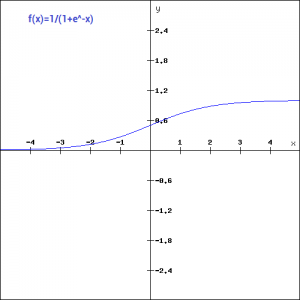
\includegraphics[scale=0.4]{./tex/fondamentaux/sigmoid.png} &
         b) 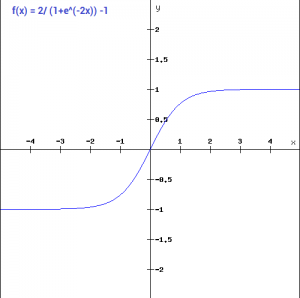
\includegraphics[scale=0.4]{./tex/fondamentaux/tanh.png} &
         c) 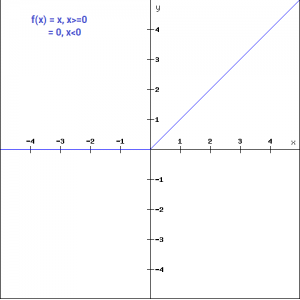
\includegraphics[scale=0.4]{./tex/fondamentaux/relu.png}  \\
         d) 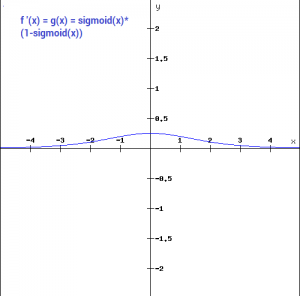
\includegraphics[scale=0.4]{./tex/fondamentaux/sigmoidder.png} &
         e) 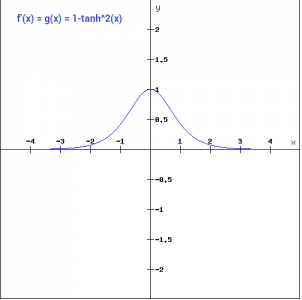
\includegraphics[scale=0.4]{./tex/fondamentaux/tanhder.png} &
         f) 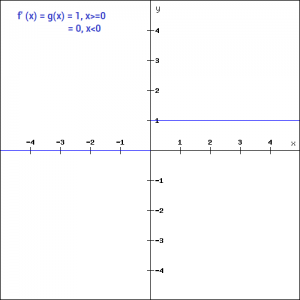
\includegraphics[scale=0.4]{./tex/fondamentaux/reluder.png}
    \end{tabular}
\caption{Fonctions d'activation: a) Sigmoide, b) tanh, c) ReLu et leurs dérivées associées}
\label{fig:my_label}
\end{figure}

\begin{itemize}
    \item Fonction Sigmoide: $f(x)=\frac{1}{1+e^-x}$\\

    La fonction sigmoide est une référence historique en tant que fonction d'activation et reste aujourd'hui, très utilisée. Elle est appréciée pour sa dérivée non constante, ce qui permet d'avoir un gradient variable selon la valeur et donc, une convergence plus performante. Néanmoins, le fait qu'elle soit positive la rend peu performante sur certains problèmes. De plus, cette fonction favorise le phénomène de \textit{vanishing gradient}\footnote{Cette notion sera étudiée par la suite}. Un effet de bord est aussi présent. En effet, au-delà de (-3,3), la valeur de la dérivée est très faible ce qui impliquera un gradient faible. Un gradient très faible limitera grandement les variations des poids et augmentera le temps d'apprentissage du neurone (voire le "freezera").\\

    Cette fonction est souvent utilisée sur la couche de sortie pour représenter une prédiction sous forme de probabilité (car résultat entre 0 et 1). C'est la fonction de référence dans le cadre de la classification binaire probabiliste.\\

    \textbf{Remarque}: Un perceptron avec la sigmoide comme fonction d'activation est identique à une régression logistique\footnote{Soyez fier de vous. Nous venons de réinventer la roue !}.

    \item Fonction tanh: $f(x) =\frac{e^x-e^{-x}}{e^x+e^{-x}}$\\

    La fonction tanh présente les mêmes caractéristiques que la fonction sigmoide. La différence se situe sur le fait qu'elle est symétrique en 0 et prend valeur dans (-1,1), ce qui lui permet de ne pas être limitée par une condition de valeur positive. De plus, on observe un pic plus prononcé sur sa dérivée, ce qui implique un gradient plus important. Ceci est une qualité et un défaut car selon le problème, ça peut accélérer la convergence ou, au contraire, l'empêcher de pleinement converger.

    \item Fonction ReLu: $f(x)=\left\{\begin{array}{ll}0 \ si \ x<0 \\max(0,x) \ si \ x\geq 0\end{array}\right.$\\

    La fonction ReLu est, aujourd'hui, la fonction d'activation la plus employée dans les réseaux de neurones au niveau des couches cachées\footnote{Cette fonction présente peu d'intérêt en couche de sortie du fait de son faible pouvoir explicatif}. Cette fonction présente des particularités très importantes dans le cadre des réseaux profonds. Nous l'étudierons en profondeur dans la suite de cette introduction.

    \item Fonction Softmax: $\delta(z)_j=\frac{e^{z_j}}{\sum_{i=1}^{N}e^{z_i}}$ avec $z=(z_1,...,z_N)$ et $j \in [1,...,N]$ \\

    La fonction Softmax est une version généralisée de la fonction Sigmoide. Elle est ainsi utilisée dans la couche de sortie pour des problèmes de classifications multi-classes (voir Section \ref{multiclasslabel}) avec représentation probabiliste. Elle est employée lorsque la couche de sortie possède différents neurones associés aux classes prédites afin d'extraire la classe dont la probabilité est la plus élevée.
\end{itemize}

\subsection{Descente du gradient et optimizeur}
\label{optimizer}

Dans la section \ref{backward}, nous avons observé que la correction appliquée sur les poids est dépendante de l'erreur totale du réseau. Il est important de définir comment cette erreur est calculée. Pour cela, il y a trois approches complémentaires: la détermination du nombres de données d'apprentissage analysées pour une même itération, la détermination du pas d'apprentissage optimal et la méthode de calcul du gradient.

\subsubsection{Approche par Batch, Minibatch et Stochastique}
Le calcul du gradient se présente sous trois formes distinctes dépendant du nombre de données d'apprentissage utilisées pour déterminer une valeur de gradient à rétro-propager.\\

\paragraph{Approche par Batch}

\noindent L'approche par batch correspond à la version originale du calcul du gradient. Cette approche utilise l'intégralité des données d'apprentissage avant de faire une rétro-propagation (une mise à jour des poids). Ainsi, l'erreur du réseau correspond à la moyenne de l'erreur réalisée par les prédictions de l'intégralité des données d'apprentissage.\\

\noindent Supposons la métrique \textit{Mean Squared Error} et un jeu de données de m entités, nous obtenons donc:
$$ \theta = \theta - \eta \cdot \nabla_\theta J(\theta)$$
$$ J(\theta) = \frac{1}{m}\sum_{i=1}^m(\hat{y}_i-y_i)^2$$

\noindent Cette approche tend à définir un gradient stable permettant de limiter les "convergences oscillantes" du réseau. Il permet donc, en théorie, de favoriser une convergence lissée. Néanmoins, elle tend à converger vers un minimum local moins performant du fait de la trop grande généralité du gradient\footnote{Rappelez-vous le compromis biais-variance. Trop de généralité nuit à la spécialisation du modèle !}. De plus, il est nécessaire de calculer l'intégralité des erreurs avant de réaliser une mise à jour. Bien que ces calculs puissent être parallélisés, les mises à jour des poids sont lentes et de ce fait, l'apprentissage du réseau aussi. Dans le cas de jeu de données massifs (plusieurs millions voir milliards de données), cette approche est inutilisable en temps humain.\\

\paragraph{Approche Stochastique}

\noindent L'approche stochastique calcule l'erreur avec une donnée d'apprentissage uniquement. Ainsi, il y a un apprentissage par rétropropagation à chaque prédiction réalisée durant l'apprentissage.\\

\noindent Supposons la métrique \textit{Mean Squared Error}, nous obtenons donc:
$$\theta = \theta - \eta \cdot \nabla_\theta J( \theta; x^{(i)}; y^{(i)})$$
$$ J(\theta; x^{(i)}; y^{(i)}) = (\hat{y^{(i)}}-y^{(i)})^2$$

\noindent Cette approche permet une évolution rapide du réseau du fait de la mise à jour récurrente des poids à chaque prédiction d'apprentissage. L'aspect stochastique favorise un gradient \textit{bruité} qui limite le risque de convergence précipitée vers un minimum local mais favorise aussi la convergence vers un minimum potentiellement moins performant. De plus, l'aspect bruité du gradient entraîne une forte variance dans la mise à jour des poids et de ce fait, tend à rendre l'évolution du réseau moins \textit{lissée}. Cette approche est très sensible aux données aberrantes et extrêmes. De même, il est préférable de sélectionner aléatoirement la donnée d'apprentissage afin d'éviter un biais associé à une répartition constante des données au fil des \textit{epochs}.\\

\paragraph{Approche par MiniBatch}

\noindent L'approche par MiniBatch est un compromis entre l'approche par Batch et Stochastique. Avec cette méthode, l'erreur est calculé à partir d'un sous-ensemble du jeu d'apprentissage. Cette méthode est la plus répandue aujourd'hui du fait de ses performances.\\

\noindent Supposons la métrique \textit{Mean Squared Error}, un jeu de données de m entités et un minibatch de n entités. Nous obtenons donc:
$$\theta = \theta - \eta \cdot \nabla_\theta J( \theta; x^{(i:i+n)}; y^{(i:i+n)})$$
$$ J( \theta; x^{(i:i+n)}; y^{(i:i+n)}) = \frac{1}{n}\sum_{i=1}^n(\hat{y}_i-y_i)^2$$

\noindent Cette méthode permet une plus grande robustesse et un meilleur contrôle de l'évolution du réseau que l'approche stochastique tout en conservant une mise à jour du réseau "régulière", ce qui permet une évolution du modèle plus rapide mais surtout, son exploitation. Le MiniBatch étant de taille restreinte, la problématique de convergence précipitée de l'approche par Batch est évitée. Cette méthode offre ainsi un bon compromis qui favorise les performances, de même que pour les facilités d'implémentation en limitant les problématiques de stockage des données d'apprentissage en mémoire. Néanmoins, le nombre d'entités dans le MiniBatch est un hyperparamètre important qui ne peut être défini qu'empiriquement. Par défaut, on a tendance à exploiter des minibatchs de 32 éléments ou plus afin d'avoir une significativité statistique. De même, il est préférable de sélectionner aléatoirement les données d'apprentissage afin d'éviter un biais associé à une répartition constante des données au fil des \textit{epochs}.

\subsubsection{La problématique de la détermination du pas - A FAIRE}

khjh

\subsubsection{Aperçu des optimizer}

Lors de la mise à jour des poids, le pas (facteur multiplicatif du gradient) a une grande importance. Une des grandes difficultés est de déterminer qu'elle est sa valeur optimale et ce, de manière statique ou dynamique. Dans la version initiale de l'algorithme du gradient, le pas est un hyperparamètre constant et fixé par l'utilisateur. Cette méthode s'avère difficile à optimiser et peu efficace expérimentalement.\\

\noindent Pour corriger ce problème, des améliorations (appelées \textit{optimizer}) ont été proposées. Deux facteurs d'optimisation existent: la méthode de détermination du pas d'apprentissage et l'étude du \textit{moment} des gradients. Le moment représente "l'engouement" que l'on a dans la mise à jour du gradient proposé. Supposons une succession de gradients dans la même direction\footnote{Imaginez une balle qui glisse le long d'une pente. L'énergie emmagasinée par la balle augmente avec la pente et diminue avec une montée ou un sol plat. Le moment peut être associé à l'énergie cinétique de cette balle} et de grande intensité, nous pouvons donc supposer être sur une voie de convergence favorable. De ce fait, il faut favoriser la mise à jour associée. Au contraire, si la valeur s'amoindrit ou que la direction varie, il faut limiter l'engouement de la mise à jour afin de ne pas "se perdre" (divergence ou convergence interrompue à cause d'une valeur de pas qui la bloque) . Le moment permet ainsi de limiter les oscillations durant la convergence, d'avoir une mémoire sur son évolution et d'accélérer la convergence.\\

\noindent parler de:
\begin{itemize}
    \item faire section: problematique du pas avec sgd
    \item snapshot ensemble https://arxiv.org/pdf/1704.00109.pdf
    \item second ordre, problème lgfgs http://cs231n.github.io/neural-networks-3/\#second
\end{itemize}

\paragraph{SGD Annealing}
Par défaut, la descente du gradient exploite un pas fixe. L'invariabilité du pas est une problématique majeure. En effet, un pas important ne permet pas de converger au plus bas du minimum local considéré. Un pas important aura tendance à s'extraire du minimum local ou à limiter grandement la précision de l'optimisation en se limitant à osciller entre deux positions approximatives. Un pas plus faible permet une plus grande sensibilité de l'optimisation en limitant l'impact de la variation, ce qui permet une plus grande précision. \\

\noindent Un pas important permet d'\textit{explorer} l'univers des hypothèses et permet une plus grande robustesse à la convergence vers le minimum local le plus proche. Au contraire, un pas faible permet une convergence plus précise mais est plus limité quant à sa capacité d'exploration. Intuitivement, nous pouvons considérer qu'un pas important est préférable au début d'un apprentissage afin que le réseau puisse explorer l'univers des hypothèses. Au contraire, plus le réseau apprend, plus il doit devenir précis et limiter l'exploration. Ainsi, le modèle doit optimiser la convergence vers le minimum local considéré. De ce fait, le pas doit être plus faible pour favoriser ce comportement.\\

\noindent Cette intuition mène à une amélioration de la détermination du pas. Ce dernier ne doit pas être fixe mais \textit{diminuer au cours du temps} (annealing\cite{annealing}). Ainsi, périodiquement, le pas va diminuer afin de passer d'un comportement exploratoire à un comportement de convergence.\\

\noindent La méthode de réduction périodique du pas est variable et présente une infinité de possibilités. Néanmoins, trois méthodes classiques sont répandues:
\begin{itemize}
    \item \textbf{Step decay}: Cette approche consiste à retirer une \textbf{valeur fixe} à la valeur du pas selon un critère de périodicité fixe ou une condition particulière. Le critère de périodicité de référence est le nombre d'épochs. Ainsi, par exemple, nous pouvons diminuer d'un quart la valeur du pas à chaque épochs (ou toutes les deux épochs etc...).\\

    Il est aussi possible de se baser sur une condition particulière, notamment la diminution de l'erreur d'apprentissage. Par exemple, au lieu de se baser sur le nombre d'épochs, nous pouvons définir que le pas doit être diminué lorsque l'erreur d'apprentissage stagne (qu'on peut associer à un comportement oscillant de la convergence) ou encore, qu'elle augmente. \\

    De même, il est possible de définir un critère sériel. Réduire le pas à chaque variation "néfaste" de l'erreur d'apprentissage possède les défauts d'un comportement stochastique, notamment la sur-exploitation des tendances locales qui peuvent nuire à la convergence. Appliquer la diminution du pas lorsqu'une augmentation de l'erreur d'apprentissage est présente $\beta$ fois permet de favoriser une bonne interprétation de la tendance globale. $\beta$ est un hyperparamètre qui peut être difficile à déterminer et relève essentiellement de l'instinct.

    \item \textbf{Exponential decay}: La variation par \textit{Step} se comporte comme une variation \textit{par palier}. Il peut être préférable d'avoir une variation plus lissée mais surtout à l'amplitude variable. Ainsi, retirer une valeur fixe à un pas élevé est moins impactant que retirer cette même valeur à un pas plus faible. Ainsi, il peut être préférable de retirer une valeur dépendant de la valeur actuelle du pas.\\

    Exponential decay se base sur un facteur de variation exponentiel. Ainsi, nous avons:
    $$\alpha = \alpha_0 e^{-k t}$$
    \noindent Avec $\alpha$, pas actuel, $\alpha_0$, pas initial et k, critère multiplicatif qui détermine l'impact de la varition. Il s'agit d'hyperparamètre à définir par l'utilisateur.

    \item \textbf{1/t decay}: Cette approche suit la même logique que Exponential decay. Elle est définie par:
    $$\alpha = \alpha_0 / (1 + k t )$$
    \noindent Avec $\alpha$, pas actuel, $\alpha_0$, pas initial et k, critère multiplicatif qui détermine l'impact de la varition. Il s'agit d'hyperparamètre à définir par l'utilisateur.
\end{itemize}

\noindent Dans les faits, lorsque ce type de méthode pour la détermination du pas est employée, \textbf{Step decay} est préféré car plus facilement interprétable d'un point de vue métier et pour la supervision de l'apprentissage. De plus, bien que plus efficace qu'une approche SGD classique, ces méthodes tendent à devenir obsolètes face à d'autres techniques plus sophistiquées sauf dans des cas d'architectures particulières.

\paragraph{Approche par cycle: Cyclical Learning Rate}
\noindent Une des problématiques majeures de l'optimisation par descente de gradient est la convergence vers un \textbf{minimum local}. \textit{SGD annealing}, du fait de la réduction permanente du pas durant l'optimisation, a tendance à être très sensible à ce problème. De même, la fonction de perte d'un réseau de neurones possède de nombreuses dimensions, ce qui favorise l'existence de \textbf{point-selle}. La Figure \ref{point_selle_pic} illustre les spécificités de ce type de point. Ces points sont très nocifs à la qualité de la convergence et trompent l'algorithme du gradient. Pour favoriser la convergence vers le minimum global\footnote{Il n'y a aucune certitude d'y arriver !}, une amélioration de SGD appelée Cyclical LR\cite{cyclicallr} a été proposée.\\

\begin{figure}
    \centering
    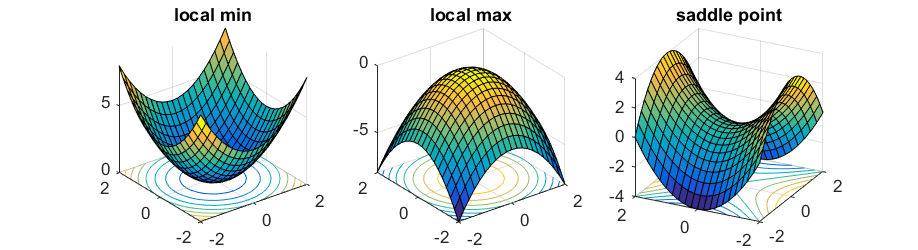
\includegraphics[scale=0.45]{./tex/fondamentaux/minmaxsaddle.png}
    \caption{Différence entre minimum global, maximum global et point-selle}
    \label{point_selle_pic}
\end{figure}

\noindent L'idée de Cyclical LR repose sur le fait d'augmenter périodiquement la valeur du pas afin de favoriser la sortie d'un minimum local instable (ou d'un point-selle). Si le minimum local (qui peut être global) est assez stable, le "pic" de la valeur du pas devrait être supporté et ne pas provoquer un changement de minimum. Le pas suit donc un comportement cyclique qui cherche à réduire sa valeur et à la rehausser périodiquement. Chaque cycle est défini par un nombre d'itérations identique et la valeur du pas est compris entre deux bornes choisies comme hyperparamètres. La variation du pas est linéaire et un cycle s'apparente à un comportement \textit{triangulaire}. Une approche parabolique et sinusoïdale ont été proposées sans amélioration notable de performance. \\

\noindent Afin de limiter le temps d'apprentissage et de "forcer" la convergence vers un minimum local, une limitation sur la borne supérieure est applicable. Elle consiste à modifier la borne supérieure pour le cycle t tel que $max_{LR_t}=\frac{max_{LR_0}}{t}$. Ainsi, le pas tend vers 0, ce qui forcera le réseau à avoir un comportement de convergence et non d'exploration. Une alternative est possible en choisissant une minoration par un facteur exponentiel, ce qui favorisera une diminution plus "lissée". Une illustration du comportement du pas est visible sur la Figure \ref{cyclicallr}.

\begin{figure}
    \centering
    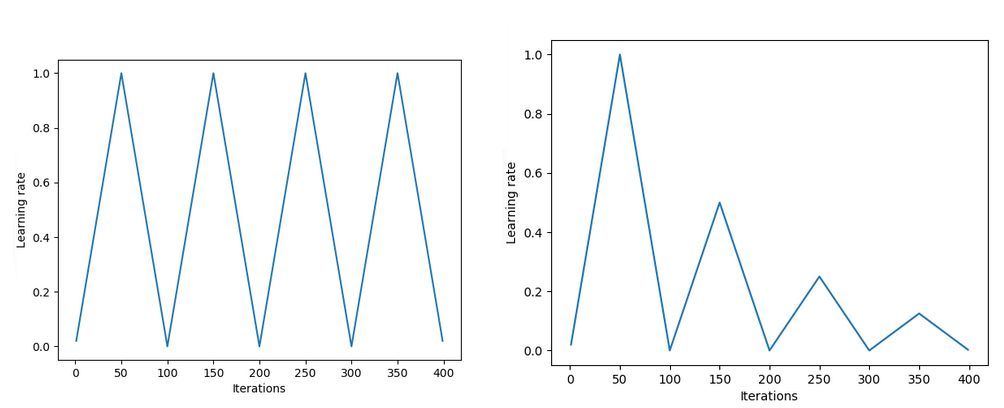
\includegraphics[scale=0.3]{./tex/fondamentaux/cyclicallr.png}
    \caption{Comportement du pas avec Cyclical LR avec une borne supérieure constante et une borne supérieure dégressive}
    \label{cyclicallr}
\end{figure}

\paragraph{Détermination des bornes supérieures et inférieures des valeurs du pas: le LR Range test}
Une contrainte de Cyclical LR est la détermination des bornes de l'intervalle des valeurs potentielles du pas. Afin de résoudre ce problème, un test a été crée: le \textbf{LR Range test}\cite{cyclicallr}.\\

\noindent Ce test consiste à définir un pas très faible, supposons $10^{-7}$ et à l'augmenter progressivement à chaque itération en observant l'impact sur le comportement de l'apprentissage. Lorsque le pas est faible, l'apprentissage stagne car la convergence est très lente. En augmentant, la convergence va se réaliser, ce qui permettra à l'erreur de diminuer. Lorsque le pas sera trop important, le modèle divergera et l'erreur augmentera. Nous pouvons ainsi observer trois régions qui permettront de définir un intervalle pertinent pour les valeurs du pas. Une illustration du test est visible sur la Figure \ref{lrrangetest}. Il est important de noter qu'il s'agit d'un test empirique et que ses résultats sont dépendants du jeux de données. L'intervalle obtenu n'est donc pas généralisable.

\begin{figure}
    \centering
    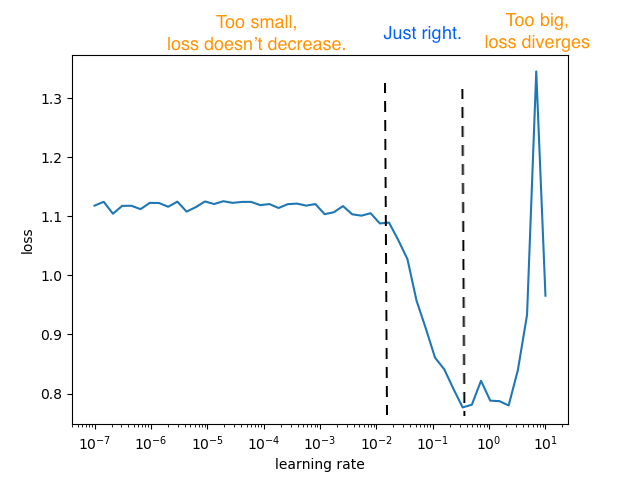
\includegraphics[scale=0.3]{./tex/fondamentaux/lrrangetest.png}
    \caption{Exemple du LR Range test}
    \label{lrrangetest}
\end{figure}

\paragraph{Approche par cycle: Exploring Stochastic Gradient Descent with Warm Restarts (SGDR)}

\noindent L'idée de SGDR\cite{sgdr} est une variante de Cyclical LR et exploite aussi une comportement cyclique. Contrairement à Cyclical LR qui possède un comportement linéaire dans la variation du pas, SGDR réalise une diminution du pas avant de le réinitialiser à la valeur de la borne supérieure, ce qui entraîne une variation non continue lors de la réinitialisation. Les bornes des valeurs du pas sont obtenues par LR Range test. Une illustration du comportement du pas est visible sur la Figure \ref{sgdr}.\\

\noindent SGDR utilise une approche \textit{cosinus annealing}\footnote{Diminution du pas selon une fonction cosinus} afin de diminuer la valeur du pas. Ainsi, pour le cycle i, le pas est égal à:
$$\eta_t=\eta_{min}^i+\frac{1}{2}(\eta_{max}^i-\eta_{min}^i)(1+cos(\frac{T_{cur}}{T_i}\pi))$$

\noindent Avec $\eta_{min}^i$, $\eta_{max}^i$, valeur minimum et maximum du pas, $T_{cur}$, le nombre d'itérations réalisées depuis la dernière réinitialisation du cycle et $T_i$, le nombre d'itérations du cycle i. Nous pouvons ainsi voir que si t=0 et $T_{cur}=0$, $\eta_t=\eta_{max}^i$. Si $T_{cur}=T_i$, alors la composante cosinus sera égale à -1 et ainsi $\eta_t=\eta_{min}^i$. $\eta_{min}^i$ et $\eta_{max}^i$ sont des hyperparamètres.\\

\noindent Afin d'améliorer les performances, il est possible d'augmenter la durée d'un cycle au fil des cycles. Pour augmenter progressivement le nombre d'itération par cycle, il est conseillé de remplacer $T_i=T_0$ par $T_i=T_0*T_{mult}$ avec $T_{mult}$, coefficient multiplicateur incrémenté à chaque cycle selon une valeur choisie. Il est possible de faire varier $\eta_{min}^i$ et $\eta_{max}^i$ selon le cycle. Cependant, pour des raisons de simplicité, il est préférable de choisir des valeurs constantes.\\

\noindent Lors de la fin d'un cycle, la valeur du poids considéré n'est pas réinitialisée mais conservée. Ainsi, si $x_t$ est la dernière valeur du poids à la fin du cycle, lors de la première itération du cycle suivant, la mise à jour du poids sera basée sur la valeur $x_t$. Cette caractéristique permet de conserver une continuité dans le comportement du poids et de ce fait, les valeurs des \textit{momentum}\footnote{Cette notion sera expliquée par la suite.} sont exploitables par exemple.

\begin{figure}
    \centering
    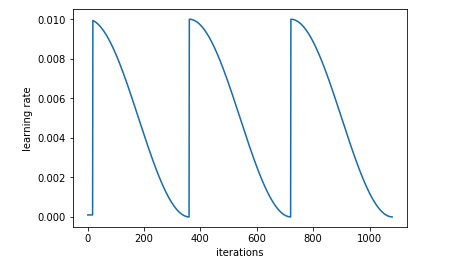
\includegraphics[scale=0.4]{./tex/fondamentaux/sgdr.png}
    \caption{Comportement du pas avec SGDR}
    \label{sgdr}
\end{figure}

\paragraph{1Cycle Policy et Super-Convergence: A FAIRE}
1cycle Policy\cite{1cyclelr}

\paragraph{Snapshot Ensembles}
\noindent Snapshot Ensembles\cite{snapshot}

\begin{figure}
    \centering
    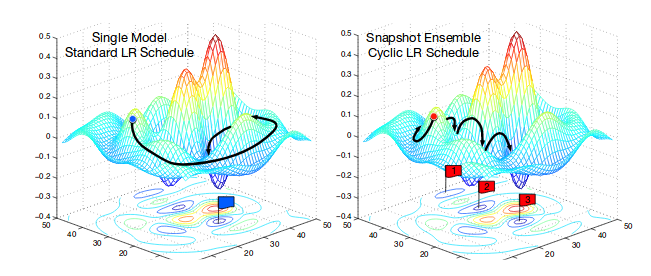
\includegraphics[scale=0.3]{./tex/fondamentaux/snapshot.png}
    \caption{Différence entre SGD et Snapshot Ensembles}
    \label{snapshot}
\end{figure}

\paragraph{Calcul du moment: Vanilla Momentum}
\noindent Cette méthode est simple. Elle est calculée en ajoutant à la valeur du gradient (pondéré par le pas), la valeur du gradient précédent pondéré par une constante qui représente l'importance associé au moment. Cette constante est un hyperparamètre choisi par l'utilisateur et souvent défini à 0.9 ou une valeur similaire\footnote{Il faut éviter que sa valeur soit supérieure à 1.}.\\

\noindent Ainsi, le gradient est défini par:
$$v_t = \gamma v_{t-1} - \eta \nabla_\theta J( \theta)$$
$$\theta = \theta + v_t $$

\paragraph{Calcul du moment: Nesterov Accelerated gradient (NAG)}
\noindent Nesterov Accelerated gradient\cite{nesterov} (NAG) est une variante du Vanilla Momentum. Alors que l'approche Vanilla Momentum n'anticipe pas ses positions futures, l'approche par Nesterov cherche à approximer la valeur future du gradient afin d'orienter son moment. L'estimation du gradient ne se fait donc plus à partir position actuelle mais à la position "prédite" après l'approximation de la position future. L'amplitude des évolutions est donc mieux maîtrisée et permet une évolution plus précise et rapide. Cette approche possède une preuve théorique plus forte, est plus efficace dans le cadre d'optimisation convexe et semble donner de meilleurs résultats expérimentaux.\\

\noindent Une illustration est visible sur la Figure \ref{nesterovm}. La mise à jour du gradient par Momentum est réalisée à partir de l'état actuel (point rouge) alors qu'avec l'approche Nesterov, la mise à jour est réalisée à partir de la position prédite (extrémité de la flèche verte). Pour plus d'explication, consulter le site \url{http://cs231n.github.io/neural-networks-3/#sgd}.

\begin{figure}
    \centering
    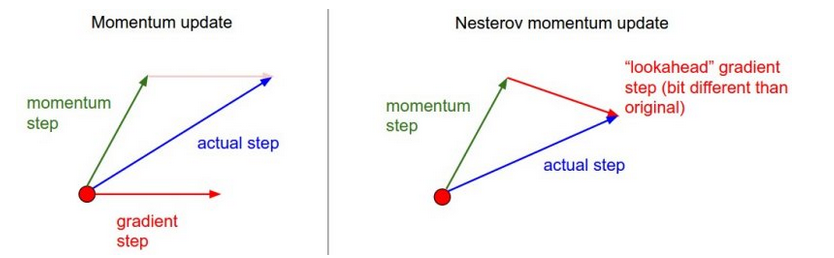
\includegraphics[scale=0.3]{./tex/fondamentaux/nesterov.png}
    \caption{Différence entre Momentum et Nesterov Momentum}
    \label{nesterovm}
\end{figure}

\noindent Ainsi, le gradient est défini par:
$$v_t = \gamma v_{t-1} - \eta \nabla_\theta J( \theta + \gamma v_{t-1} )$$
$$\theta = \theta + v_t $$

\paragraph{Méthode adaptative: Adagrad}
\noindent Adagrad\cite{adagrad} modifie le pas afin qu'il devienne dynamique et dépendant du paramètre optimisé. Ainsi, un paramètre ayant été peu modifié (en terme de variation de valeur) aura un pas important alors qu'un paramètre régulièrement mis à jour aura un pas minoré. Cette méthode nous émancipe de l'étude d'une valeur pour le pas, si ce n'est la détermination d'une valeur initiale (souvent placé à 0.01). En effet, il a été montré empiriquement qu'il est souvent plus efficace d'avoir un pas variable selon l'état du réseau.\\

\noindent Supposons une mise à jour d'un poids par une approche SGD \textit{classique}. Nous avons:
$$g_{t, i} = \nabla_\theta J( \theta_{t, i} )$$
$$\theta_{t+1, i} = \theta_{t, i} - \eta \cdot g_{t, i}$$

\noindent Dans le cas de \textit{Adagrad}, nous avons alors:
$$\theta_{t+1, i} = \theta_{t, i} - \dfrac{\eta}{\sqrt{G_{t, i} + \epsilon}} \cdot g_{t, i}$$
$$G_{t, i}=\sum_{j=1}^t g_{j, i}^2$$

\noindent Le pas est ainsi minoré selon la somme au carré de l'ensemble des gradients précédents. L'utilisation de $\epsilon$ permet d'éviter le cas interdit de la division par 0. Sa valeur est constante et très faible. $10^{-8}$ par exemple.\\

\noindent La faiblesse de cette méthode est associée au facteur uniquement dégressif de la valeur du pas. En effet, selon cet optimizer, il ne peut "que" diminuer. Ainsi, au fil des apprentissages, le pas diminuera jusqu'à devenir infinitésimal et figera le réseau. Dans le cas d'apprentissage très profond, cette limitation est très problématique car la convergence n'est pas atteinte avant le blocage du pas.

\paragraph{Méthode adaptative: AdaDelta}
\noindent AdaDelta\cite{adadelta} est une variante de Adagrad qui corrige le problème de la minoration agressive du pas. Ainsi, au lieu de considérer les différents gradients identiquement, cet optimizer se concentre sur une fenêtre des derniers gradients calculés en minorant proportionnellement les gradients selon leur ancienneté. Il propose aussi une méthode pour supprimer l'initialisation du pas, émancipant l'utilisateur d'un hyperparamètre.\\

\noindent Dans le cas de \textit{AdaDelta}, l'approche de normalisation du pas est définie par:
$$E[g^2]_t = \gamma E[g^2]_{t-1} + (1 - \gamma) g^2_t$$
$$\Delta \theta_t = - \dfrac{\eta}{\sqrt{E[g^2]_t + \epsilon}} g_{t}$$
$$\Delta \theta_t = - \dfrac{\eta}{RMS[g]_{t}} g_t$$

\noindent Ainsi, le facteur $\gamma$ s'applique récursivement sur chaque valeur de gradient selon son ancienneté et permet de maîtriser la valeur du pas\footnote{Il est conseillé d'exploiter une valeur entre 0.5 et 0.9}. Dans les faits, l'équation précédente est une approche naïve. En effet, elle présente un problème potentiel lié à l'unité de $\Delta \theta_t$. Ce problème est d'ailleurs présent avec les optimizers par moment et Adagrad.\\

\noindent Supposons une mise à jour par SGD classique pour un poids $\theta$ donné. Nous avons donc:
$$\Delta \theta = - \eta g$$

\noindent Soit $U_{\Delta \theta}$, unité de $\Delta \theta$ et f, fonction de perte. Nous avons donc:
$$U_{\Delta \theta} \propto U_{g} \propto \frac{\partial f}{\partial \theta} \propto \frac{1}{U_\theta}$$

\noindent \textbf{Remarque}: On fait l'hypothèse que la fonction de perte n'a pas d'unité.\\

\noindent On observe que les unités ne sont pas en phase. En effet, d'après l'équation de mise à jour des poids, $U_{\Delta \theta}$ devrait être égal à $U_\theta$.\\

\noindent Pour corriger cette erreur, il a été proposé de s'inspirer d'une méthode du seconde ordre telle que la méthode de Newton qui repose sur une approximation hessienne.
Ainsi, nous avons dorénavant:
$$\Delta \theta = -H^{-1} g$$

\noindent H correspond à la dérivée seconde de la fonction de perte. Ainsi, nous obtenons:
$$U_{\Delta \theta} \propto U_{H^{-1}g} \propto \frac{\frac{\partial f}{\partial \theta}}{\frac{\partial^2 f}{\partial^2 \theta}} \propto U_\theta$$

\noindent On observe que l'unité est respectée. Cette approche est donc efficace. Néanmoins, il faut définir le paramètre $H^{-1}$.

$$U_{\Delta \theta} = \frac{\frac{\partial f}{\partial \theta}}{\frac{\partial^2 f}{\partial^2 \theta}}$$
$$\frac{1}{\frac{\partial^2 f}{\partial^2 \theta}}=\frac{U_{\Delta \theta}}{\frac{\partial f}{\partial \theta}}$$
$$H^{-1}=\frac{U_{\Delta \theta}}{\frac{\partial f}{\partial \theta}}$$

\noindent D'où:
$$\Delta \theta =\frac{U_{\Delta \theta}}{\frac{\partial f}{\partial \theta}}g$$

\noindent D'après l'équation obtenue par l'approche naïve, nous avons:
$$\Delta \theta_t = - \dfrac{\eta}{RMS[g]_{t}} g_t$$

\noindent Il reste à modifier le numérateur afin de respecter l'unité. Pour cela, nous pouvons utiliser la même approche que pour le dénominateur soit:
$$E[\Delta \theta^2]_t = \gamma E[\Delta \theta^2]_{t-1} + (1 - \gamma) \Delta \theta^2_t$$
$$RMS[\Delta \theta]_{t} = \sqrt{E[\Delta \theta^2]_t + \epsilon}$$

\noindent Nous avons donc:
$$\Delta \theta_t = -\dfrac{RMS[\Delta \theta]_{t}}{RMS[g]_{t}} g_{t}$$

\noindent Malheureusement, la valeur $RMS[\Delta \theta]_{t}$ est inconnue. Afin de l'approximer, on fait l'hypothèse que la courbe est \textit{localement} lisse. Nous pouvons donc approximer la valeur en exploitant la valeur jusqu'à la dernière mise à jour soit $\Delta \theta_{t-1}$.

\noindent Ainsi:
$$\Delta \theta_t =  -\dfrac{RMS[\Delta \theta]_{t-1}}{RMS[g]_{t}} g_{t}$$
$$\theta_{t+1} = \theta_t + \Delta \theta_t $$

\noindent Cette approche est une version "simplifiée" d'une vraie optimisation par méthode de second ordre. En effet, calculer une inversion de matrice est une opération lourde ($O(n^3))$ et ne peut être exploitée. On observera qu'il n'y a plus d'hyperparamètre à définir. On supposera une valeur nulle à $\Delta \theta_0$. \\

\paragraph{Méthode adaptative: RMSprop}
\noindent Cet optimizer est équivalent à la version naïve d'AdalDelta. Les hyperparamètres sont fixés selon l'équation suivante:
$$E[g^2]_t = 0.9 E[g^2]_{t-1} + 0.1 g^2_t$$
$$\theta_{t+1} = \theta_{t} - \dfrac{\eta}{\sqrt{E[g^2]_t + \epsilon}} g_{t} $$

\paragraph{Méthode adaptative: Adam}
Adam\cite{adam_and_max} est une approche adaptative qui exploite la moyenne des gradients au carré (comme Adadelta et RMSprop) mais aussi la moyenne des gradients. Ainsi, il réalise une estimation de la moyenne (1er moment) et de la variance non centrée du gradient (2nd moment). L'estimation respecte une approche dépréciative selon la position du gradient antécédent.\\

\noindent Adam est défini par:
$$m_t = \beta_1 m_{t-1} + (1 - \beta_1) g_t$$
$$v_t = \beta_2 v_{t-1} + (1 - \beta_2) g_t^2 $$

\noindent $\beta_1$ et $\beta_2$ sont des hyperparamètres et déterminent le pas dépréciatif des gradients antécédents.\\

\noindent Les deux moyennes sont initialisées à 0. De ce fait, leurs estimations sont biaisées (notamment durant les premières itérations). Afin de corriger les estimations, les valeurs non biaisées sont calculées selon:

$$\hat{m}_t = \dfrac{m_t}{1 - \beta^t_1}$$
$$\hat{v}_t = \dfrac{v_t}{1 - \beta^t_2}$$

\noindent La mise à jour du paramètre est appliquée selon:

$$\theta_{t+1} = \theta_{t} - \dfrac{\alpha}{\sqrt{\hat{v}_t} + \epsilon} \hat{m}_t$$

\noindent $\epsilon$ apporte une solution au cas insoluble en $t=0$ qui impose une division par 0, ce qui n'est pas réalisable. $\alpha$ est un hyperparamètre comparable au pas d'apprentissage (régulé par le comportement des gradients précédents). Les créateurs de cet optimizer estime qu'une bonne initialisation par défaut pour les différents hyperparamètres serait: $\beta_1=0.9$, $\beta_2=0.999$, $\epsilon=10^{-8}$ et $\alpha=0.001$.\\

\noindent \textbf{Remarque}: Il est possible de réécrire l'équation de manière plus efficiente. En effet, il est équivalent de définir l'équation de mise à jour telle que:

$$\alpha_t=\alpha \frac{\sqrt{1-\beta_2^t}}{1-\beta_1^t}$$
$$\theta_{t} = \theta_{t-1} - \dfrac{\alpha_t m_t}{\sqrt{v_t} + \epsilon}$$

\noindent Lors de la mise à jour des poids, la dernière itération est souvent bruitée à cause des approximations stochastiques. Afin d'obtenir une meilleure généralisation, un \textit{moyennage} est souvent réalisé. Il a été montré que SGD converge mieux avec $\overline{\theta_t}=\frac{1}{t}\sum_{k=1}^n\theta_k$. Dans le cadre de Adam, une alternative basé sur une moyenne dépréciative (nommée \textit{Temporal Averaging}) peut être appliquée telle que:
$$\overline{\theta_t}=\beta_2\overline{\theta}_{t-1}+(1-\beta_2)\theta_t$$

\noindent Nous appliquons $\overline{\theta_0}=0$. Cette initialisation est biaisée. L'estimation non biaisée est définie par: $\Hat{\theta_t}=\frac{\overline{\theta_t}}{(1-\beta_2^t)}$.\\


\noindent Aujourd'hui, cet optimizer fait office de choix par défaut lorsque aucun autre optimizer présente un intérêt particulier ou qu'aucune étude n'a été faite pour définir le meilleur choix à réaliser. Bien expérimentalement rapide à converger, il est souvent critiqué pour être d'une grande inefficacité dans le cadre de certaines thématiques ou d'être trop sensible à la problématique du minimum local.

\paragraph{Méthode adaptative: AdaMax}
Dans la cadre d'Adam, le facteur $v_t$ est inversement proportionnel à la norme $l_2$ des gradients précédents (via la valeur $v_{t-1}$). AdaMax\cite{adam_and_max} est une variante de Adam qui généralise en utilisant la norme $l_p$. Nous avons donc:

$$v_t = \beta_2^p v_{t-1} + (1 - \beta_2^p) |g_t|^p$$

\noindent Lorsque p augmente, les normes tendent à devenir numériquement instables d'où l'exploitation de la norme $l_1$ et $l_2$. Cependant, la norme $l_\infty$ présente une stabilité exploitable en plus d'une facilité d'implémentation.\\

\noindent Ainsi, nous obtenons:
$$u_t = \underset{p \rightarrow \infty}{lim} (v_t)^{1/p} = \beta_2^\infty v_{t-1} + (1 - \beta_2^\infty) |g_t|^\infty$$
$$u_t = \max(\beta_2 \cdot v_{t-1}, |g_t|)$$

$$\theta_{t+1} = \theta_{t} - \dfrac{\alpha}{u_t} \hat{m}_t$$

\noindent \textbf{Remarque}: l'équation précédente peut être réecrite telle que:
$$\theta_{t} = \theta_{t-1} - \frac{\alpha}{(1-\beta_1^t)u_t}m_t$$

\noindent De même, le correctif \textit{Temporal Averaging}\footnote{Voir algorithme Adam.} est applicable pour cet algorithme.  Les créateurs de cet optimizer estime qu'une bonne initialisation par défaut pour les différents hyperparamètres serait: $\beta_1=0.9$, $\beta_2=0.999$, $\epsilon=10^{-8}$ et $\alpha=0.002$.\\

\paragraph{Méthode adaptative: Nadam}
Nadam\cite{Nadam} est une variante de Adam qui exploite \textit{Nesterov Accelerated gradient} (NAG) au lieu de \textit{Vanilla Momentum}. \\

\noindent Pour rappel, \textit{Vanilla Momentum} est défini par:
$$g_t = \nabla_{\theta_t}J(\theta_t)$$
$$m_t = \gamma m_{t-1} + \alpha g_t$$
$$\theta_{t} = \theta_{t-1} - m_t$$

\noindent NAG réalise une estimation plus précise en évaluant la valeur du gradient en considérant le moment du gradient et non uniquement $\theta_t$. Ainsi, NAG est défini par:
$$g_t = \nabla_{\theta_{t-1}}J(\theta_{t-1} - \gamma m_{t-1})$$
$$m_t = \gamma m_{t-1} + \alpha g_t$$
$$\theta_{t} = \theta_{t-1} - m_t$$

\noindent On peut observer que le moment est exploité \textbf{deux fois}: lors de la mise à jour du gradient et lors du calcul de $\theta_{t}$. Afin de simplifier l'implémentation de Nadam, une alternative a été proposée. Elle permet de calculer le moment de l'itération $t+1$ à l'itération t:
$$g_t = \nabla_{\theta_{t-1}}J(\theta_{t-1})$$
$$m_t = \gamma m_{t-1} + \alpha g_t$$
$$\theta_{t} = \theta_{t-1} - (\gamma_{t+1} m_t + \alpha_t g_t)$$

\noindent Pour rappel, Adam est défini par:
$$m_t = \beta_1 m_{t-1} + (1 - \beta_1) g_t$$
$$\hat{m}_t = \frac{m_t}{1 - \beta^t_1}$$
$$\theta_{t} = \theta_{t-1} - \frac{\alpha_t}{\sqrt{\hat{v}_t} + \epsilon} \hat{m}_t$$

\noindent En réecrivant l'approche \textit{Vanilla Momentum} de Adam par remplacement des variables, nous obtenons l'équation suivante (avec application du correctif de biais):
$$\theta_{t} = \theta_{t-1} - \dfrac{\alpha_t}{\sqrt{\hat{v}_t} + \epsilon} (\dfrac{\beta_{1,t} m_{t-1}}{1 - \beta^{t}_1} + \dfrac{(1 - \beta_{1,t}) g_t}{1 - \beta^t_1})$$

\noindent En appliquant l'approche NAG, nous avons dorénavant:
$$\theta_{t} = \theta_{t-1} - \dfrac{\alpha_t}{\sqrt{\hat{v}_t} + \epsilon} (\dfrac{\beta_{1,t+1} m_{t}}{1 - \beta^{t+1}_1} + \dfrac{(1 - \beta_{1,t}) g_t}{1 - \beta^t_1})$$

\noindent Cette approche est applicable aux autres méthodes adaptatives comme Adamax par exemple.

\paragraph{Adam et correctifs théoriques - AdamW}

\noindent Pour favoriser une bonne convergence, différentes méthodes de régulation sont exploitées. La plus répandue est la régularisation par la norme $L_2$ (Voir la partie \ref{l2_reg} pour plus d'informations). Pour rappel, cette régularisation s'applique sur la fonction de perte et est définie par:
$$ \mathcal{L}_{L_2}=\mathcal{L} + \alpha \norm*{\mathcal{L}}_2^2$$

\noindent Une autre forme de régularisation existe et est très employée dans le cadre des optimizers. Elle se nomme \textit{Weight Decay}\cite{weight_decay}. Contrairement à l'approche par norme (qui agit sur la fonction de perte), \textit{Weight Decay} agit directement sur la valeur du paramètre lors de sa mise à jour en imposant une minoration. Ainsi, lors d'une mise à jour, le paramètre $\theta$ sera défini par:
$$\theta_{t+1}=(1-\lambda)\theta_t-\alpha \nabla \mathcal{L}(\theta_t)$$

\noindent Dans les faits, ces deux méthodes sont similaires. A tel point qu'elles sont équivalentes dans le cadre de l'optimizer SGD.\\

\noindent \textbf{Preuve}: \\

\fbox{\parbox{\textwidth}{Supposons une approche SGD régularisée par la norme $L_2$ telle que:
$$ \mathcal{L}_{L_2}=\mathcal{L} + \frac{\lambda'}{2} \norm*{\theta}_2^2$$

\noindent Lors de la mise à jour d'un poids, nous avons donc:
$$ \theta_{t+1}=\theta_t - \alpha \nabla \mathcal{L}_{L_2}(\theta_t)=\theta_t - \alpha \nabla \mathcal{L}(\theta_t) - \alpha \lambda' \theta_t$$

\noindent Supposons SGD avec l'approche \textit{Weight Decay}:
$$\theta_{t+1}=(1-\lambda)\theta_t-\alpha \nabla \mathcal{L}(\theta_t)$$

\noindent Les deux approches sont identiques si $\lambda'=\frac{\lambda}{\alpha}$\\}}\\

\noindent Du fait de cette équivalence, la régularisation par norme est souvent considérée  comme \textit{équivalente} à la régulation par Weight Decay. Or, ce n'est \textbf{pas vrai}. Notamment dans le cas des méthodes adaptatives telles que Adam.\\

\noindent Dans de nombreuses implémentations de l'algorithme Adam, appliquer Weight Decay est identique à utiliser la régularisation $L_2$. En d'autres mots, lors de l'utilisation de $L_2$/Weight Decay sur Adam, la valeur $g_t$ devient égale à\footnote{Vous référer à la partie sur Adam pour le détail de l'optimizer Adam (et vous remémorer les notations !)}:
$$g_{t+1,reg}=\nabla \mathcal{L}(\theta_{t})+\lambda \theta_t$$
$$\theta_{t+1} = \theta_{t} - \dfrac{\eta}{\sqrt{\hat{v}_t} + \epsilon} \hat{m}_t$$

\noindent Afin de corriger cette erreur, AdamW\cite{adamw} a été proposé et implémente correctement Weight Decay. Ainsi, avec AdamW, nous obtenons:
$$g_{t+1}=\nabla \mathcal{L}(\theta_{t})$$
$$\theta_{t+1,reg} = \theta_{t} - \dfrac{\eta}{\sqrt{\hat{v}_t} + \epsilon} \hat{m}_t + \lambda \theta_{t}$$

\noindent Définir le facteur de Weight Decay est difficile. Néanmoins, il a été montré qu'une petite taille de batch accentue l'effet du Weight Decay. Afin de limiter le risque lié à cette dépendance, il est préférable de normaliser $\lambda$ afin de limiter le risque de biais. Pour cela, il a été proposé:
$$\lambda_{norm}=\lambda*\sqrt{\frac{b}{BT}}$$

\noindent Avec b, dimension du batch, B, nombre  totale de données d'apprentissage, T, nombre d'epochs. Cette normalisation est instinctive. Il est probable qu'il soit possible de proposer une amélioration notable à cette approche.\\

\noindent Bien que simple, AdamW permet une amélioration notable des performances de l'optimizer Adam. De plus, il est suspecté que SGD soit meilleure que Adam sur certaine problématique du fait de cette erreur théorique de généralisation de la norme $L_2$.

\paragraph{Adam et correctifs théoriques - AMSGrad}

\noindent Les algorithmes adaptatifs basées sur une moyenne pondérée présente une faiblesse théorique. Supposons la valeur $\Gamma_{t+1}$ tel que:
$$v_t = \beta_2 v_{t-1} + (1 - \beta_2) g_t^2$$
$$\Gamma_{t+1}=\frac{\sqrt{v_{t+1}}}{\alpha_{t+1}}-\frac{\sqrt{v_{t}}}{\alpha_{t}}$$

\noindent Afin de limiter le risque de convergence indésirable, il est nécessaire que $\Gamma_t$ soit défini positif, i.e $\Gamma_t \succeq 0$ pour tout t. Or, ce n'est pas le cas avec Adam\footnote{Consultez l'article \cite{amsgrad} pour la démonstration mathématique de ce résultat.}.\\

\noindent Cette observation peut laisser penser que Adagrad est une approche, qui, au final, est préférable. Ce n'est pas le cas car la diminution du pas est trop agressive avec cette approche. Il est donc nécessaire de proposer une alternative qui respecte la condition sur $\Gamma_t$ tout en limitant l'agressivité de la diminution imposée.\\

\noindent AMSGrad\cite{amsgrad} est une variante de Adam et respecte la condition sur $\Gamma_t$. Au lieu d'exploiter la moyenne pondérée des gradients passés $v_t$, il utilise le \textit{maximum} des gradients passés, i.e $\hat{v}_t = \text{max}(\hat{v}_{t-1}, v_t)$. De plus, $\beta_1$ est variable et décroissant (par exemple $\beta_{1,t}=\beta_1/t$).\\

\noindent \textbf{Remarque}: Dans l'article de référence, l'utilisation de $\beta_1$ est floue. Le paramètre est considéré comme fixe dans les démonstrations mais variable dans la définition de l'algorithme. Dans les faits, il semblerait que le comportement du coefficient $\beta_1$ soit peu important pour l'efficacité globale de AMSGrad. Néanmoins, une valeur décroissante semble avoir une démonstration théorique confirmée du fait d'articles complémentaires supposant cette condition.\\

\noindent Supposons le cas où $v_{t-1}>g_t^2 > 0$. Adam va provoquer une augmentation agressive du pas d'apprentissage (diminution de $v_t$). Au contraire, Adagrad va diminuer le pas d'apprentissage (augmentation de $v_t$) car il exploite une somme non pondérée. Par opposition, AMSGrad ne va pas modifier le pas d'apprentissage, assurant une meilleure stabilité.\\

\noindent Une explication intuitive peut être donnée à ce résultat pouvant sembler contre-intuitif. Il a été observé que des minibatchs porteurs d'informations utiles sont existants mais rares. De ce fait, leur influence est diminuée car écrasée par la moyenne pondérée. L'utilisation d'une moyenne pondérée provoque un phénomène de mémoire à \textit{court terme} qui limite l'impact des minibatchs utiles, ce qui est désastreux dans le cadre de certaines problématiques.\\

\noindent Ainsi, AMSGrad est défini par:
\begin{align*}
\begin{split}
\beta_{1} &= \beta_{1,1}\\
\beta_{1,t} &= \beta_{1}\lambda^{t-1}\\
m_t &= \beta_{1,t} m_{t-1} + (1 - \beta_{1,t}) g_t \\
v_t &= \beta_2 v_{t-1} + (1 - \beta_2) g_t^2\\
\hat{v}_t &= \text{max}(\hat{v}_{t-1}, v_t) \\
\theta_{t+1} &= \theta_{t} - \dfrac{\eta}{\sqrt{\hat{v}_t} + \epsilon} m_t
\end{split}
\end{align*}

\noindent Une autre variante a aussi été proposée pour satisfaire la condition $\Gamma_t$. Nommée ADAMNC, elle est strictement identique à Adam si ce n'est que $\beta_2$ est \textbf{non constant}. Nous avons donc:
\begin{align*}
\begin{split}
\beta_{1} &= \beta_{1,1}\\
\beta_{1,t} &= \beta_{1}\lambda^{t-1}\\
\beta_{2,t} &= 1-1/t\\
\end{split}
\end{align*}

\noindent Cette approche permet de pondérer différemment l'ensemble des gradients passés. Dans le cadre de ADAMNC, la pondération est constante (si $\beta_2$ est défini comme précédemment), i.e $v_{t,i}=\sum_{j=1}^{t}g^2_{j,i}/t$.

\paragraph{Adam et correctifs théoriques - Nostalgic Adam}

Nostalgic Adam\cite{nosadam} (NosAdam) propose une autre approche pour exploiter les gradients passés afin de calculer le pas d'apprentissage. La particularité est que les gradients anciens ont un poids plus importants que les gradients récents. Pour cela, il est nécessaire de définir des conditions particulières sur la détermination de $\beta_{2,t}$. NosAdam respecte la condition de semi-positivité de $\Gamma_t$. Elle a donc une solidité théorique avérée.

\noindent Ainsi, NosAdam est défini par:
\begin{align*}
\begin{split}
B_t&=\sum_{k=1}^t b_k, \ b_k >0, \ t \geq 1,  B_0=0\\
\beta_{2,t} &=B_{t-1}/B_t\\
m_t &= \beta_{1} m_{t-1} + (1 - \beta_{1}) g_t \\
v_t &= \beta_{2,t} v_{t-1} + (1 - \beta_{2,t}) g_t^2\\
\theta_{t+1} &= \theta_{t} - \dfrac{\eta}{\sqrt{\hat{v}_t} + \epsilon} m_t
\end{split}
\end{align*}

\noindent \textbf{Remarque}: La détermination de $\beta_1$ est imprécise dans l'article de recherche. Il est variable dans le cadre des démonstrations théoriques mais l'écriture de l'algorithme sous-entend qu'il est constant. Une certaine tolérance doit être envisageable sur ce paramètre...\\

\noindent La condition $\beta_{2,t}=B_{t-1}/B_t$ est une écriture générale. Il a été démontré que la condition de semi-positivité est vérifiée si $B_t/t$ n'est pas croissant, i.e $b_k$ non croissant et $b_k>0$. Elle est notamment avérée lorsque $\beta_{2,t}$ est indépendant des données et uniquement lié à t. \\

\noindent Supposons $\beta_{2,t} =B_{t-1}/B_t$ et $B_t=\sum_{k=1}^t b_k$. De ce fait, nous avons:
$$v_t=\sum_{k=1}^t \frac{b_k}{B_t}g_k^2$$

\noindent $b_k$ est le poids relatif de $g_k^2$. Or, $b_k$ est non croissant donc les gradients anciens sont majorés par rapport aux récents. Cette approche est l'opposé de la méthode par moyenne pondérée qui majore les gradients récents.\\

\noindent Il est intéressant de noter que les créateurs de NosAdam considère ADAMNC comme un cas particulier de NosAdam. En effet, ADAMNC est défini pour $B_{2,t}=1-1/t$. De ce fait, $v_t=\sum_{k=1}^t \frac{g_k^2}{t}$. On observe qu'il n'y a plus de pondération relative donc que chaque gradient est pondéré identiquement. De même, AMSGrad, à travers l'opérateur max(.), conserve une mémoire \textit{longue-durée} des gradients passés et peut réaliser une pondération importante d'un gradient passé grâce aux spécificités de max(.)\footnote{Il y a une dépendance vis-à-vis de $g_k^2$. En effet, il n'y a pas mémoire du passé dans sa globalité mais que de l'évènement principal caractérisé par max(.). Il s'agit donc d'une mémoire long-terme sélective en plus d'être exclusive.}.\\

\noindent NosAdam définit une classe d'optimizers caractérisée par des conditions sur $\beta_2$. Un cas particulier de NosAam a été proposé: NosAdam-HH. Cette approche exploite une série \textit{hyper-harmonique} pour définir $b_k$ tel que $b_k=k^{-\lambda}$ avec $\lambda \geq 0$.

\paragraph{Méthode adaptative cyclique - AdamWR}

Les optimizers cycliques présentent une efficacité remarquable grâce à leur capacité à s'extraire des minimums locaux peu performants. AdamWR\cite{adamw} propose d'unir AdamW avec \textit{Cosinus Annealing and Warm Restarts}.\\

\noindent AdamW modifie Adam tel que:
$$\theta_{t+1,reg} = \theta_{t} - \dfrac{\eta}{\sqrt{\hat{v}_t} + \epsilon} \hat{m}_t + \lambda \theta_{t}$$

\noindent Dans le cadre de AdamWR, nous avons dorénavant:
$$\theta_{t+1,reg} = \theta_{t} - \alpha_t(\dfrac{\eta}{\sqrt{\hat{v}_t} + \epsilon} \hat{m}_t + \lambda \theta_{t})$$
$$\alpha_t=\alpha_{min}^{(i)}+0.5(\alpha_{max}^{(i)}-\alpha_{min}^{(i)})(1+cos(\frac{\pi T_{cur}}{T_i})) $$

\noindent Avec $\alpha_{min}^{(i)}$ et $\alpha_{max}^{(i)}$, valeur minimale et maximale de $\alpha$ durant l'i-ième restart. Pour limiter le nombre d'hyperparamètre, il est commun de considérer ces valeurs comme fixes mais il a été montré que proposer une ajustation à chaque restart pourrait potentiellement améliorer les performances. $T_{curr}$ correspond au nombre d'itérations depuis le dernier restart et $T_i$, le nombre total d'itérations durant le i-ième restart.\\

\noindent Afin d'améliorer cet algorithme, il est préférable d'utiliser une valeur $T_i$ variable selon le nombre de restarts réalisés. Intuitivement, il est préférable d'avoir des restarts réguliers au début de l'apprentissage mais plus rare au fil du temps afin de favoriser une convergence. De ce fait, il est préférable que $T_i$ soit croissant au fil des itérations. Cette pratique est standard dans le cadre des optimizers cycliques. De même, il est nécessaire d'utiliser une valeur \textit{normalisée} du facteur de Weight Decay\footnote{Voir AdamW pour plus d'informations sur cette normalisation.} (dans le cadre du Warm Restarts, nous considérerons T comme nombre d'itération dans le restart actuel). \\

\noindent AdamWR présente une efficacité globalement similaire à AdamW mais sa vitesse de convergence est significativement meilleure. AdamWR rivalise avec SGDWR en terme de performance, ce qui illustre l'hypothèse que les mauvaises performances de Adam sur certains problèmes pourraient être liées à la confusion entre $L_2$/Weight Decay.

\paragraph{Discriminative Fine-Tuning}

\noindent Discriminative Fine-Tuning\cite{dis_fine_tun} est une approche complémentaire aux méthodes vues précédemment qui évalue le pas d'apprentissage selon le comportement vis-a-vis des données\footnote{Le gradient est directement lié aux données d'apprentissage.}.\\

\noindent Les méthodes précédentes considèrent que chaque couche exploite un même pas d'apprentissage pour mettre à jour ses poids. Or, ce postulat est contestable. En effet, les couches les plus basses (les premières couches du réseau) discriminent des phénomènes généralistes\footnote{Par exemple, dans le cadre de l'analyse d'une image, les premières couches discrimineront des structures géométriques simples comme des droites, courbes, cercles etc...}. De ce fait, ces couches sont faiblement spécialisées car non liées à la tâche à discriminer. Par exemple, supposons le cas de l'analyse d'image. Peu importe le type d'objet à discriminer sur les images, son analyse exploitera toujours des structures géométriques simples et récurrentes car chaque phénomène aussi complexe soit-il repose sur des structures simples communes. Ainsi, le comportement discriminant est réalisé essentiellement par les couches les plus hautes (les dernières couches du réseau) qui analysent des structures plus complexes et donc, spécialisées.\\

\noindent Cette observation conditionne l'idée que seule les dernières couches possèdent un vrai pouvoir discriminant. De ce fait, il est nécessaire que les modifications induites par l'exploitation du gradient soit plus importantes pour les couches hautes que les couches basses. En effet, le gradient étant lié aux données et donc au phénomènes observés, il a donc un lien plus fort avec les couches hautes. Ainsi, Discriminative Fine-Tuning propose de modifier le pas d'apprentissage selon la position de la couche mise-à-jour. Les couches les plus hautes auront un pas majoré et les couches les plus basses, un pas minoré. Une illustration est visible sur la Figure\footnote{Les spécificités d'une architecture CNN seront développées dans la suite de cette introduction.} \ref{dfn_cnn}.\\

\begin{figure}
    \centering
    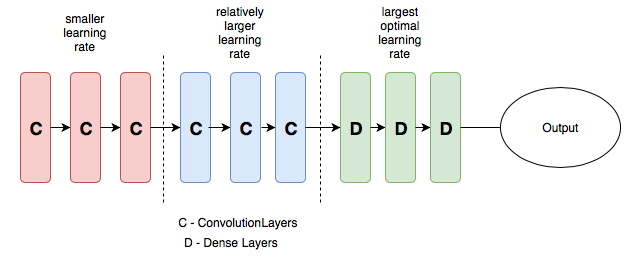
\includegraphics[scale=0.35]{./tex/fondamentaux/cnn_fintun.png}
    \caption{Discriminative Fine-Tuning sur un réseau CNN standard}
    \label{dfn_cnn}
\end{figure}

\noindent Plus formellement, supposons un réseau avec L couches. Nous définissons $\theta=\{\theta_0,...,\theta_l,...,\theta_L\}$, les paramètres du réseau avec $\theta_l$, paramètres de la l-ième couche. Alors:
$$\theta_t^l=\theta_{t-1}^l - \eta^l\nabla_{\theta^l}J(\theta)$$

\noindent Avec $\eta^{l-1}=\eta^l/2.6$ avec $\eta^L=\eta_{max}$ tel que $\eta_{max}$ est la valeur du pas obtenu par l'optimizer choisi (par exemple, Adam). Le facteur 2.6 est un résultat obtenu empiriquement. Il est donc utile de considérer une étude approfondie du meilleur facteur possible selon le type de tâche à accomplir.\\

\noindent \textbf{Remarque}: Dans les faits, cette méthode n'est pas utilisée lorsque l'apprentissage est \textit{from-scratch}\footnote{Un apprentissage from-scratch est un apprentissage à partir de rien, i.e une initialisation aléatoire des poids du réseau.}. En effet, dans cette situation, les poids des couches basses sont aléatoires. De ce fait, les couches basses sont incapables de discriminer un quelconque phénomène. Il est donc nécessaire de les entraîner comme les couches plus hautes.\\

\noindent Au contraire, l'idée de pondérer le pas d'apprentissage est très exploitée lors d'un \textit{apprentissage par transfert}. En effet, dans cette configuration, le réseau initial n'est pas \textit{from scratch} mais déjà entrainé sur une tâche. Le comportement des couches basses n'est donc plus aléatoire mais apte à une discrimination. Ce cas particulier sera étudié dans la suite de cette introduction.


\paragraph{Et les méthodes d'optimisation du 2nd ordre ? - A FAIRE}

\paragraph{SGD, calcul distribué et parallélisation - A FAIRE}

\paragraph{Inférence de l'optimizer - Neural Optimization Search}
PowerSign and AddSign \cite{learninggrad2}

\paragraph{Inférence de l'optimizer - LSTM approach}
LSTM-Learning\cite{learninggrad}

\paragraph{Quel optimizer choisir ?}

\noindent C'est toujours une question \textbf{sans réponse} ! La liste présentée est non-exhaustive et l'étude des optimizer est encore un sujet de recherche actuel. Il n'existe pas de hiérarchie de performance clairement établie. Seule l'approche empirique est exploitée aujourd'hui. Néanmoins, les méthodes avec un \textit{learning rate} adaptatif semblent être les plus répandues, notamment Adam malgré des performances parfois très mauvaises. L'état de l'art tend à exploiter des approches cycliques bien qu'elles ne soient pas encore pleinement démocratisées. Néanmoins, il n'est pas rare d'observer l'emploi de SGD (avec Momentum) dans des publications actuelles, notamment pour des tâches de traduction (analyse de texte).\\

\noindent \textbf{Important}: A l'heure actuelle, la recherche est encore très manuelle et intuitive, i.e l'homme propose et expérimente lui-même des concepts qu'il invente. Néanmoins, des travaux récents exploitent l'intelligence artificielle pour apprendre à découvrir les concepts performants. Un aperçu a été proposé avec l'inférence de l'optimizer mais cette pratique se généralise avec l'auto-apprentissage de l'architecture d'un réseau dans sa globalité. Cette approche est encore expérimentale mais promet d'être une semi-révolution dans l'exploitation du Deep Learning et de sa Recherche de part la facilité d'innovation et d'expoitation (pour l'industrie) qui en découle.

\subsubsection{Gradient noise}

Afin de favoriser la robustesse du réseau face à des stimulations ambiguës ou inhabituelles, il est intéressant de \textit{bruiter}\cite{gauss_deep} la valeur du gradient durant l'apprentissage afin de renforcer le réseau. Cette approche consiste à ajouter un bruit gaussien (distribution gaussienne centrée en 0 et écart-type variable) à la valeur du gradient calculé à chaque rétropropagation. Ainsi, supposons $g_{i,t}$, le gradient obtenu pour le poids i à l'instant t, alors $g_{i,t,gauss}= g_{i,t} + \mathcal{N}(0,\sigma^2)$ avec $\sigma^2_t = \dfrac{\eta}{(1 + t)^\gamma}$ et $\eta \in [0.01,0.3,1.0]$.\\

\noindent Ainsi, le bruit sera plus important en début d'apprentissage pour forcer le réseau à ne pas converger trop rapidement vers un minimum local\footnote{Favoriser l'exploration des solutions possibles}. Cette méthode serait performante pour les modèles très profonds, limiterait l'impact d'une mauvaise initialisation des poids du réseau et favoriserait "l'échappement" des minimum locaux (qui sont de plus en plus nombreux alors que le modèle s'approfondit). Cette méthode, bien qu'élégante, n'est que peu employée par la recherche et son efficacité incertaine.

\subsubsection{Gradient Clipping}
Afin de limiter le risque d'explosion du gradient (phénomène nommé \textit{exploding gradient}\footnote{Voir Section \ref{explodsec}}), il est pertinent de borner la valeur du gradient en normalisant sa valeur absolue lorsqu'elle dépasse un seuil défini. Cette méthode est appelée \textit{Gradient Clipping}\cite{clip_deep}. Il existe plusieurs manières de réaliser cette normalisation bien que la majorité des implémentations se limitent à l'utilisation d'une valeur seuil, i.e $|g_{i,t}|>\lambda \Rightarrow |g_{i,t}| = \lambda$. Cette approche est reconnue comme efficace au fil des publications de recherche.

\subsection{ReLu et les dangers du gradient}
\label{relu_danger}
Le gradient est l'élément central pour l'apprentissage d'un réseau de neurones. Cependant, trois dangers majeurs sont à considérer pour garantir l'intégrité des gradients: \textbf{Exploding Gradient, Vanishing Gradient et Dead ReLu}.\\

\noindent Un réseau de neurone peut avoir des centaines (ou plus) couches associées à des milliers (ou plus) neurones. De ce fait, le modèle peut être très profond. Nous avons vu que l'apprentissage se base sur la rétropropagation du gradient. Cette rétropropagation est un produit de facteur. Ainsi, plus le poids à mettre à jour est éloignée de la sortie du réseau (couches basses du réseau), plus le degrés du produit est élevé. Cette particularité peut poser problème selon l'architecture du réseau (notamment la profondeur) ou les fonctions de transfert dont la dérivée est comprise dans $[0,1[$ ou strictement supérieure à 1 sur un intervalle quelconque.

\subsubsection{Vanishing Gradient}
\noindent Dans le cas où la valeur des dérivées partielles des couches intermédiaires est comprise dans $[0,1[$, il y a un risque de \textit{vanishing gradient}. En effet, pour n dans $[0,1[$, $\prod_{k=1}^\infty \alpha_n \underset{\infty}{\longrightarrow} 0$. Cette particularité peut figer le réseau et annuler la mise à jour de neurones éloignés car la mise à jour du poids est infinitésimale.

\subsubsection{Exploding Gradient}
\label{explodsec}
\noindent Au contraire, pour des valeurs comprises dans $]1,\infty[$, il y a un risque d'\textit{exploding gradient}. Pour n dans $]1,\infty[$, $\prod_{k=1}^\infty \alpha_n \underset{\infty}{\longrightarrow} \infty$. Ainsi, la valeur du gradient "explose" et peut empêcher une bonne convergence du modèle (évolution du poids trop importante) voire annuler l'apprentissage du réseau avec des valeurs dites NaN (Not A Number) car dépassant les limites matérielles de la représentation des nombres par ordinateur.

\subsubsection{Fonction ReLu et Dead ReLU}
\label{dead_relu}
\paragraph{Les avantages et le danger de ReLU}
\noindent Pour corriger cette difficulté, une fonction d'activation est souvent utilisée pour les couches cachées des réseaux: la fonction ReLu.\\

\noindent La fonction ReLu est définie par: $f(x)=\left\{\begin{array}{ll}0 \ si \ x<0 \\max(0,x) \ si \ x\geq 0\end{array}\right.$\\

\noindent Sa dérivée est nulle sur $]\infty,0]$ et égale à 1 sur $]0,\infty[$. De part les valeurs de sa dérivée, le risque d'exploding gradient est annulé. Néanmoins, la présence d'une dérivée nulle peut laisser penser que le risque de vanishing gradient est présent. Bien que vrai, ce défaut est compensé par la capacité de ReLu à rendre le réseau éparse.\\

\noindent Le risque de sur-apprentissage\footnote{Voir Section \ref{surappsec}} est présent lorsque les neurones deviennent trop inter-dépendants, que ce soit durant la prédiction ou l'apprentissage. L'idée principale, soutenue par l'analogie biologique du cerveau, est que le réseau doit être localement stimulé pour répondre à une entrée. Ainsi, selon l'entrée, l'ensemble du réseau ne doit pas être activé mais seulement une sous-partie capable d'interpréter cette stimulation. La fonction ReLU, nulle pour tout x négatif, permet de simuler ce comportement. De plus, la dérivée de ReLu, semblable à une fonction \textit{Porte}, permet de réaliser des mises à jour éparses du réseau. La présence d'une dérivé nulle (pour x négatif) permet de limiter localement la mise à jour des poids, rendant les évolutions du système localisées et moins inter-dépendantes. En cas de stimulation positive, la dérivée étant de 1, l'influence sur la valeur du gradient est nulle. Cette fonction d'activation permet ainsi d'éteindre des neurones durant la phase de prédiction et force le réseau à avoir une stimulation localisée pour réaliser la prédiction. Durant la rétropropagation, son comportement orchestre les régions du réseau qui apprennent et celles qui dorment. Ainsi, cette fonction permet d'agir sur l'architecture du réseau pour limiter les problèmes de corrélation néfastes entre les neurones qui favorisent le sur-apprentissage. De plus, cette limitation des neurones employés permet de limiter le coût de calcul et ainsi, d'augmenter la vitesse du réseau (en prédiction et apprentissage).\\

\noindent Ces spécificités ont popularisé la fonction ReLu qui est, aujourd'hui, la fonction de référence pour les couches cachées des réseaux neuronaux. Elle est peu employée pour la couche de sortie car elle ne présente que peu de pouvoir explicatif. Les fonction sigmoide/softmax sont préférées pour leur représentation probabiliste ou encore la fonction linéaire standard pour une représentation sans norme spécifique.\\

\noindent Néanmoins, cette fonction est sensible au phénomène appelé \textit{Dead ReLu}. En effet, la dérivée (localement) nulle de la fonction ReLu présente des caractéristiques dangereuses. En effet, dans le cas d'initialisation du réseau avec des poids mal calibrés, il est possible que la stimulation soit fortement négative (peu importe la données d'apprentissage), provocant une sortie nulle permanente du neurone. La dérivée étant nulle, le neurone n'apprend pas (gradient nul) et de ce fait, la sortie ne pourra jamais être autre que nulle durant tout l'apprentissage. Ce comportement est associé à un "neurone mort": le neurone n'apprend pas et retourne une sortie nulle en tout temps. Cette particularité peut entraîner l'inactivité d'une partie plus ou moins importante du réseau et nuire à son efficacité voire le condamner. Afin de lutter contre ce problème, l'utilisation de \textit{Régularisation}\footnote{Voir Section \ref{regsec}} en plus d'une bonne initialisation\footnote{Voir Section \ref{init_weight}}) sont employées.\\

\noindent Afin de lutter contre ce phénomène, des améliorations ont été proposées pour la fonction ReLu (un graphique récapitulatif est visible sur la Figure \ref{elurelu}):

\begin{figure}
    \begin{tabular}{cc}
    \centering
       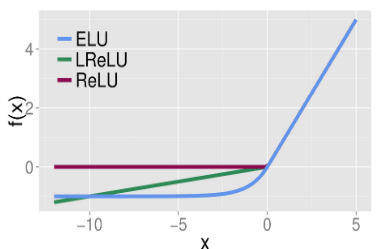
\includegraphics[scale=0.4]{./tex/fondamentaux/reluelu.png}  & 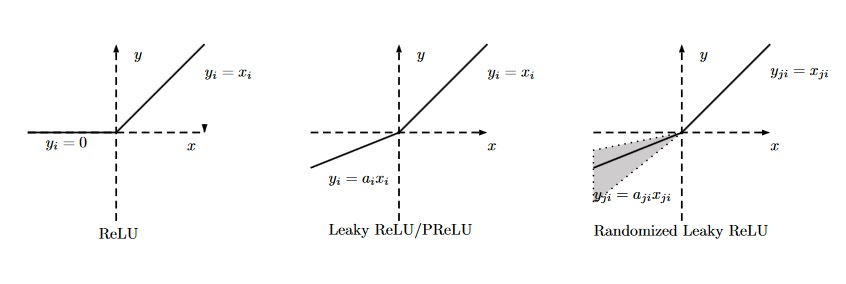
\includegraphics[scale=0.4]{./tex/fondamentaux/relupic.jpg} \\
    \end{tabular}
    \caption{Fonction ReLu et ses Variantes}
    \label{elurelu}
\end{figure}


\paragraph{Leaky ReLU (LReLU)}
LReLU\cite{randorelu} est définie par: $f(x)=\left\{\begin{array}{ll}\alpha x \ si \ x<0 \\max(0,x) \ si \ x\geq 0\end{array}\right.$ avec $\alpha$ petit (souvent inité à 0.01).\\

\noindent Cette variante permet de conserver la capacité d'apprentissage du neurone en supprimant la possibilité de gradient nul. Néanmoins, la valeur de la dérivée reste très faible (égale à $\alpha$), ce qui peut demander un temps d'apprentissage important pour ré-activer le neurone. De plus, elle demande la détermination d'un nouveau hyperparamètre.

\paragraph{Randomized ReLU (RReLU)}
RReLU\cite{randorelu} est définie par: $f(x)=\left\{\begin{array}{ll}\alpha^{(\mathcal{U}_i)} x \ si \ x<0 \\max(0,x) \ si \ x\geq 0\end{array}\right.$ avec $\alpha^{(\mathcal{U}_i)}$, valeur aléatoire issue d'une distribution uniforme $\mathcal{U}(m,n)$ avec m < n et $[m,n] \in [0,1[$.\\

\noindent Lors de l'apprentissage, $\alpha^{(\mathcal{U}_i)}$ varie à chaque itérations. Lors du l'évaluation (test) du modèle ou de prédiction, la valeur de $\alpha^{(\mathcal{U}_i)}$ est fixé. L'objectif de l'aléatoire est de diminuer le risque de sur-apprentissage du réseau.

\paragraph{Parameterized ReLU (PReLU)}
PReLU\cite{prelu_raw}\cite{randorelu} est semblable à Leaky ReLu mais le coefficient $\alpha$ est calculé dynamiquement par backpropagation. Ainsi, $\alpha$ n'est plus un hyperparamètre mais demande un coût de calcul supérieur (très négligeable). PReLu est définie par:

$$f(x_i)=\left\{\begin{array}{ll}\alpha_i x_i \ si \ x_i<0 \\max(0,x_i) \ si \ x_i\geq 0\end{array}\right.$$

\noindent Le paramètre $\alpha_i$ peut être appris selon deux approches:
\begin{itemize}
    \item \textbf{Local}: L'approche locale exploite un coefficient $\alpha_i$ pour chaque channel de la couche correspondante. Il y aura donc autant de paramètres appris que de \textit{feature map} en sortie de la couche.\\

    \item \textbf{Global}: L'approche globale exploite un coefficient $\alpha$ unique pour l'ensemble des channels de la couche, ce qui diminue le nombre de paramètres à apprendre durant l'apprentissage.
\end{itemize}

\noindent Expérimentalement, les deux approches ont des résultats similaires même si l'approche \textit{locale} est légèrement plus performante. Pour les deux approches, le coût computationnel est négligeable car $nbr_{poids} \gg nbr_{\alpha_i}$. Néanmoins, il serait intéressant d'étudier l'impact des deux configurations vis-à-vis du sur-apprentissage et de la capacité de généralisation du modèle.\\

\noindent Le paramètre $\alpha_i$ est entrainé par backpropagation. Ainsi, la mise à jour de sa valeur est dépendante de son gradient. Dans le cadre de l'approche locale, nous avons:

$$\frac{\partial \varepsilon}{\partial \alpha_i}=\sum_{x_i}\frac{\partial \varepsilon}{\partial f(x_i)}\frac{\partial f(x_i)}{\partial \alpha_i}$$

$$\frac{\partial f(x_i)}{\partial \alpha_i}=\left\{\begin{array}{ll}x_i \ si \ x_i<0 \\0 \ si \ x_i\geq 0\end{array}\right.$$

\noindent Avec $\varepsilon$ représentant la fonction de coût. La somme $\sum_{x_i}$ est appliquée car on exploite l'erreur selon l'ensemble des positions de la \textit{feature map}\footnote{Ne pas oublier le comportement de fenêtre glissante dans les réseaux convolutifs. Ainsi, le même neurone est appliqué à chaque position de la feature map considérée, ce qui nécessite de sommer les résultats pour apprendre sur l'erreur globale de l'analyse de la feature map.}.

\noindent Dans le cadre de l'approche globale,  nous obtenons:

$$\frac{\partial \varepsilon}{\partial \alpha}=\sum_{i}\sum_{x_i}\frac{\partial \varepsilon}{\partial f(x_i)}\frac{\partial f(x_i)}{\partial \alpha}$$

\noindent L'erreur est ainsi généralisée sur l'ensemble des channels et sommées pour en extraire sa valeur.\\

\noindent La mise à jour du paramètre suit une approche \textit{momentum} et est caractérisée par:
$$\alpha_{i}^{k+1}=\beta \alpha_i^{k}+\epsilon \frac{\partial \varepsilon}{\partial \alpha_i^k}$$

\noindent Avec $\beta$, coefficient du \textit{momentum} et $\epsilon$, pas d'apprentissage. \\

\noindent Il est intéressant de noter qu'aucune régularisation n'a été appliquée (notamment $l_2$) car elle a tendance à forcer $\alpha_i$ à tendre vers 0, ce qui rend PReLU comparable à Relu. De plus, sa valeur est non bornée. Néanmoins, expérimentalement, il semble qu'il n'y ait pas de phénomène d'\textit{explosion} de la valeur du coefficient\footnote{La valeur dépasse rarement 1 d'après les expérimentations des créateurs de PReLU.}. Par défaut, l'initialisation de $\alpha_i$ est à 0.25.

\paragraph{Exponential ReLU (ELU)}
ELU\cite{elu} est définie par: $f(x)=\left\{\begin{array}{ll} \alpha(exp(x)-1) \ si \ x<0 \\max(0,x) \ si \ x\geq 0\end{array}\right.$\\

\noindent Cette fonction permet de borner la valeur d'activation pour $x<0$, augmentant ainsi sa résistance au bruit. Le facteur $\alpha$ est un hyperparamètre fixé.

\paragraph{Concatenated ReLU (CReLU)}

Expérimentalement, il a été montré que les filtres des premières couches d'un réseau tendent à être redondants afin d'extraire l'information issue des \textit{phases} positives et négatives d'un signal donné. Cette faiblesse oblige le réseau à exploiter d'autres filtres pour exploiter l'information perdue par l'application d'une fonction d'activation ReLU (perte de l'information de la phase négative). Par exemple, sur la Figure \ref{phasefilter}, nous pouvons observer un couple de filtres. Le comportement des filtres est similaire mais opposé par la phase. Afin de limiter la redondance de filtre, Concatenated ReLU propose d'extraire l'information intégralement sans la perte imposée par ReLU en considérant aussi les valeurs négatives selon la même approche que ReLu possède avec les valeurs positives.\\

\noindent CReLU\cite{crelu} est ainsi définie par: $f(x)=(max(0,x), max(0, -x))$.\\

\noindent  Elle est très similaire à Absolute Value Rectification (AVR) mais au lieu d'additionner les deux sorties intermédiaires, CReLU les concatène. De ce fait, la sortie de cette fonction d'activation est de profondeur 2. Cette fonction d'activation permet ainsi de limiter le nombre de filtres nécessaires en optimisant l'extraction d'informations d'un signal donné.

\begin{figure}
\centering
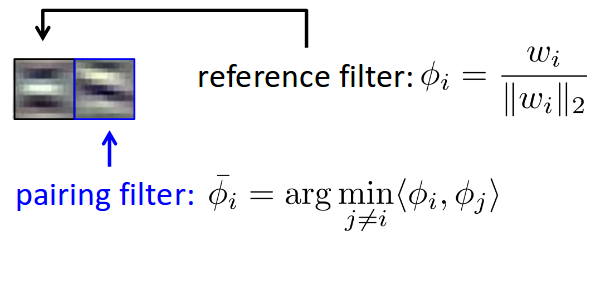
\includegraphics[scale=0.4]{./tex/fondamentaux/filterphase.png}
\caption{Exemple de deux filtres de phase opposée}
\label{phasefilter}
\end{figure}

\paragraph{Scaled Exponential Linear Units (SeLU)}: \\
La fonction est définie par: $f(x)=\lambda\left\{\begin{array}{ll} \alpha(exp(x)-1) \ si \ x<0 \\max(0,x) \ si \ x\geq 0\end{array}\right.$\\

\noindent  \textbf{Attention}: Cette partie nécessite la connaissance des fondamentaux d'architecture d'un réseau profond.\\

\noindent  Cette fonction est une des composantes utilisée dans le cadre des Self-Normalizing Neural Networks\cite{snn} (SNN). Cette architecture propose une autre approche afin de résoudre la problématique de la normalisation des données dans les réseaux très profonds. Au lieu d'employer des méthodes de normalisation externes\footnote{Comme le Batch Normalisation par exemple} appliquées à la sortie d'une fonction d'activation, la sortie de la fonction d'activation fournit des valeurs déjà normalisées. Pour que cette spécificité soit réalisée, il est nécessaire d'employer des fonctions SELU initialisées selon la distribution $W\sim \mathcal{N}\big(0,\frac{\textbf{1}}{n_{in}}\big)$. Cette distribution est comparable aux distributions standards (MSRA/Xavier par exemple) mais la variance n'exploite pas le facteur 2 qui neutralise les effets de la fonction d'activation. Pour plus de détails, notamment mathématiques, veuillez vous référer à l'article associé \cite{snn}\footnote{C'est un article très mathématique et lourd à la lecture !}.

\subsection{Initialisation des hyperparamètres - A FAIRE}
\subsubsection{Initialisation des poids}
\label{init_weight}
L'initialisation des poids d'un réseau est un critère important à considérer. Une mauvaise initialisation peut provoquer la divergence de réseau, notamment dans le cas de réseau profond. Il est donc important de réaliser une initialisation limitant ce danger. L'objectif de l'initialisation est de faire en sorte que les sorties des neurones aient approximativement la même variance, de même que pour les valeurs des gradients obtenus par rétropropagation. Plusieurs approches ont été popularisées ces dernières années:\\

\noindent \textbf{Basé sur la variance des sorties de neurones uniquement}:

\begin{itemize}
    \item \textbf{Calibration de la variance}: L'initialisation avec calibration de la variance revient à choisir aléatoirement une valeur dans une distribution normale définie par: $W\sim \mathcal{N}\big(0,\frac{1}{n_{in}}\big)$ avec $n_{in}$, nombre d'entrées du neurone (ou nombre de neurones sur la couche précédente).\\

    \item \textbf{ReLu Calibration}: La fonction ReLu est la fonction d'activation la plus populaire et utilisée actuellement (pour les couches cachées). Son étude est encore un sujet de recherche important et dynamique. Une publication récente \cite{relu_deep} préconise une initialisation telle que: $W\sim \mathcal{N}\big(0,\frac{2}{n_{in}}\big)$ ou via une distribution uniforme: $W\sim U\big[-\sqrt{\frac{6}{n_{in}}},\sqrt{\frac{6}{n_{in}}}\big]$.\\

    La distribution normale est la distribution standard pour initier les poids associées à la fonction ReLu.
\end{itemize}

\noindent \textbf{Basé sur un compromis entre la variance des sorties de neurones et des gradients}:

\begin{itemize}
    \item \textbf{Xavier initialization}: D'autres approches préconisent un compromis entre la variance des sorties des neurones et des gradients calculés par rétropropagation. La méthode préconisée devient ainsi une dépendante du nombre d'entrées et de sorties d'un neurone\footnote{Lors de la rétropropagation, ce sont les sorties des neurones qui sont exploitées}. La première approche correspond à une distribution normale: $W\sim \mathcal{N}\big(0,\frac{2}{n_{in}+n_{out}}\big)$ et la seconde, une distribution uniforme: $\mathbb{W}\sim U\big[-\frac{\sqrt{6}}{\sqrt{n_{in}+n_{out}}},\frac{\sqrt{6}}{\sqrt{n_{in}+n_{out}}}\big]$.
\end{itemize}

\noindent \textbf{Important}: Par défaut, il est \textbf{important} d'éviter les initialisations aléatoires sur un intervalle \textit{élevé}, de même qu'initialiser à 0 l'ensemble des poids (sauf spécificité d'une méthode).

\subsubsection{Initialisation et détermination des hyperparamètres - A FAIRE}
%http://cs231n.github.io/neural-networks-3/#distr

\subsection{Jeu d'apprentissage et spécificités}
Une des plus grandes contraintes du Deep Learning est la création d'un jeu de données d'apprentissage\footnote{On utilise souvent l'anglicisme \textit{dataset}} de \textit{qualité}. La notion de \textit{qualité} repose sur différents critères:
\begin{itemize}
    \item \textbf{Spécialisation}: Un jeu de données doit se focaliser sur le phénomène qu'il représente. Par exemple, si l'on souhaite détecter des chats sur une image, il est évident que le jeu de données d'apprentissage devra contenir des chats...
    \item \textbf{Représentativité}: Un jeu de données doit être capable de représenter le phénomène sous toutes ses formes (tout du moins un maximum) afin de rendre la discrimination représentative de ses différentes hypothèses possibles. Supposons un jeu de données pour discriminer tout type de chats. Il est donc intéressant d'avoir des données variables selon:
    \begin{itemize}
        \item \textbf{Spécificité du phénomène}: La première condition est de représenter un maximum de spécificité que peut possède le phénomène. Par exemple, dans le cas d'un chat, il est intéressant de mêler des chats de différentes races, tailles, couleurs, posture et mouvement etc...
        \item \textbf{Spécificité du contexte}: Le phénomène ne sera pas toujours représenté de manière centrée sur l'image tout en occupant la majorité de sa surface. C'est ainsi nécessaire de considérer des cas où le phénomène est localisé sur une sous-partie de l'image. Il est donc important d'avoir des images de l'environnement où se développe le contexte. Par exemple, en supposant le cas des chats, il est utile d'avoir des cas où la présence du chat est plus (ou moins) importante\footnote{La localisation des zones devrait être uniformément (idéalement) distribuée}, une diversité d'environnement (un chat dans un appartement, dans la rue,...)
        \item \textbf{Spécificité du capteur}: Selon le capteur, la nature de l'image peut varier indépendamment du phénomène et de son environnement. Un appareil haute définition ne donnera pas la même qualité d'image qu'une caméra standard. Il est donc nécessaire de considérer cette spécificité en exploitant des images issues de sources différentes.
        \item \textbf{Spécificité de détérioration}: Il est possible qu'une image soit détériorée (capteur défectueux, présence de bruit, etc...). Exploiter des données bruitées permet donc de renforcer la robustesse du modèle.
    \end{itemize}
    \item \textbf{Biais et Indépendance}: Cet aspect est un sujet de recherche intense et un des piliers de l'\textit{Ethique} de l'Intelligence Artificielle. Afin d'apprendre, un modèle (tout comme un être humain) devra posséder des biais de décision. Comprendre parfaitement et prévenir des dérives prédictives (comme les \textit{prédictions auto-génératrices}) nécessitera la maîtrise et la détection de ces biais. Il est ainsi pertinent d'étudier les biais que possède notre jeu d'apprentissage (en considérant les particularités des méthodes d'apprentissage de l'algorithme utilisé) en les détectant dans un premier cas et si possible, les supprimer (ou modifier) si ils représentent un danger. Réaliser cette analyse est encore un travail immature et non abouti mais \textbf{capital} à moyen-terme.
\end{itemize}

\subsection{Prédiction multi-label et multi-classe}
\label{multiclasslabel}
\subsubsection{Généralités}
La caractérisation \textit{multi-classe} / \textit{multi-label} est généralement réalisée dans le cadre d'une tâche de classification.\\

\noindent Une classification est caractérisée comme \textit{mono-classe} lorsqu'elle ne discrimine qu'une classe. Il s'agit donc d'une classification binaire (Est / N'est pas). Au contraire, dans le cas d'une classification \textit{multi-classe}, le réseau doit discriminer plusieurs classes afin de prédire les caractéristiques de l'entité inférée.\\

\noindent L'architecture du réseau est dépendante du type de classification souhaitée. En effet, dans le cadre d'une classification binaire, un seul neurone de sortie est nécessaire. Ce neurone aura pour fonction de calculer $P(Y_{i,classe}| X_i, \theta)$, i.e la probabilité que l'entité i soit de la classe $Y_{classe}$ sachant ses caractéristiques X et l'architecture du réseau définie par $\theta$.\\

\noindent Au contraire, dans le cadre d'une tâche multi-classe, le réseau doit prédire n probabilités associées aux n classes définies. De ce fait, le réseau doit être capable de prédire $\underset{j \in [1,n]}{P(Y_{i,classe_{j}}| X_i, \theta)}$.\\

\noindent Un neurone est capable de prédire la probabilité associée à une classe. Pour prédire n probabilités associées à n classes, il est donc nécessaire d'avoir n neurones sur la couche de sortie.\\

\noindent On parle de classification \textit{multi-classe} lorsque le modèle discrimine plusieurs classes mais qu'une entité ne peut être associée qu'à \textbf{une} classe uniquement, i.e les classes sont \textbf{mutuellement exclusives}. Par exemple, supposons un modèle de classification multi-classe capable de discriminer les chats et les chiens, les entités inférées par ce modèle seront classées comme chat \textbf{ou} comme chien uniquement. Or, le modèle théorique présenté précédemment calcule $\underset{j \in [1,n]}{P(Y_{i,classe_{j}}| X_i, \theta)}$. Pour respecter le cadre de la classification multi-tâche, le réseau doit dont être modifié pour calculer $argmax(\underset{j \in [1,n]}{P(Y_{i,classe_{j}}| X_i, \theta))}$.\\

\noindent Au contraire, on parle de classification multi-label lorsqu'une entité peut être définie par \textbf{plusieurs classes}. Elles ne sont donc pas exclusives. Par exemple, un homme à vélo peut être catégorisée comme \textit{homme} et \textit{cycliste}. De ce fait, la classification multi-label, au contraire de la classification multi-classe, n'impose pas l'utilisation de \textit{argmax}.\\

\noindent En résumé, la classification \textit{multi-classe} prédit positivement une unique classe parmi un ensemble de classes alors que la classification \textit{multi-label} en prédit positivement aucune, une (ou plusieurs) parmi un ensemble de classes.\\

\noindent La différence d'architecture entre ces deux approches repose essentiellement sur la fonction d'activation de la couche de sortie. Ainsi, dans le cadre d'une classification \textit{multi-classe}, la couche de sortie sera associée à une activation par la fonction \textit{softmax} qui permet d'extraire la probabilité la plus élevée en plus de respecter la condition d'exclusion. Néanmoins, cette fonction impose $\sum_i P(Y_i | X) = 1$. Cette hypothèse est plus \textit{forte} que la condition d'exclusion. En effet, elle impose que l'\textit{univers} corresponde à l'ensemble des classes du modèle, ce qui est une contrainte forte. \\

\noindent Au contraire, dans le cadre d'une classification multi-label, chaque neurone de la couche de sortie sera associé à la fonction \textit{sigmoïde} qui permet de calculer la probabilité d'appartenance à une classe indépendamment pour chaque classe. Chaque classe étant indépendante des autres, il n'y a pas d'impératif de somme égale à 1.\\

\noindent \textbf{Remarque}: La fonction \textit{softmax} extrait la probabilité la plus forte proportionnellement aux valeurs de l'ensemble de probabilités obtenues\footnote{L'utilisation de \textit{softmax} impose l'hypothèse que chaque entité puisse être caractérisée par une classe du modèle.}. De ce fait, une classe est nécessairement prédite \textit{positivement} bien qu'il soit possible que l'entité analysée ne corresponde pas à une des classes du réseau. Par exemple, supposons un réseau capable de discriminer les cyclistes et les chats. Si on présente un chien, le réseau déterminera des probabilités faibles pour les classes cyclistes et chats. Néanmoins, la fonction \textit{softmax} prédira nécessairement des probabilités indépendamment de la valeur "absolue" de ces prédictions. La classe prédite sera probablement chat car un chat "ressemble plus" à un chien qu'à un cycliste. Comme un chien ressemble bien plus à un chat qu'à un cycliste, \textit{softmax} prédira une probabilité élevée pour la classe \textit{chat}. Cette particularité impose de créer une classe \textit{neutre} qui correspond à une entité non caractérisée par les autres classes. Ainsi, si un modèle discrimine n classes, dans les faits, il devra en discriminer n+1 pour considérer la possibilité d'une image non associée à une de ces classes.\\

\noindent Au contraire, la classification \textit{multi-label} repose sur la valeur absolue des probabilités et non la valeur relative entre ces probabilités. Chaque probabilité étant indépendante, il est tout à fait possible qu'une prédiction de ce type de réseau soit négative pour chacune des classes. Ainsi, il n'y a pas d'impératif à la création d'une classe \textit{neutre}. \\

\noindent Bien que l'approche \textit{multi-label} soit plus souple et modulable, elle est plus dure à exploiter dans le cadre de l'apprentissage. L'approche \textit{multi-classe} est souvent préférée lorsque le problème traité le permet.

\subsubsection{Prédiction et distribution de données}
La difficulté principale de la prédiction \textit{multi-classe} (ou \textit{multi-label}) est associée à la distribution des données d'apprentissage. En effet, il est possible qu'elle soit très déséquilibrée avec, par exemple, une classe fortement majoritaire et d'autres minoritaires. Cette particularité du jeu d'apprentissage induira un biais dans l'apprentissage qui peut être responsable d'un échec critique de l'apprentissage. Ce type de problématique est très répandu, notamment dans les tâches de détection d'entités rares qui sont très présentes dans le domaine médicale par exemple.\\

\noindent Supposons une tâche qui consiste à détecter les tweets \textit{toxiques} et à les classifier selon différentes catégories (acharnement, contenu sexuel, discrimination raciale). Nous supposerons qu'un tweet peut appartenir à plusieurs catégories. Nous sommes donc dans le cadre d'une prédiction \textit{multi-label}.\\

\noindent Notre jeu d'apprentissage correspond à un ensemble de tweets obtenus sur un intervalle continu et dont les tweets sont labellisés sans considération de leurs particularités (sain ou toxique). Il est évident que la majorité des tweets sont "sains" et de ce fait, non classifiés dans les sous catégories de toxicité. Ainsi, la majorité des tweets d'apprentissage sont négatifs pour chacune de ces classes, i.e présentent un vecteur de label égal à $[0, 0, 0]$. Nous supposerons les sous-catégories comme uniformément distribuées et la répartition sain/toxique équivalente à 95\%-5\%. \\

\noindent Le risque principal induit par ce type de données déséquilibrées est la (possible) convergence vers un minimum local sans pouvoir explicatif. En effet, nous avons 95\% des données classées comme sain. Ainsi, si le modèle considère que toute donnée est saine, alors il aura 95\% de bonne prédiction sur son jeu d'apprentissage. Les données d'apprentissage associées à un tweet toxique étant rares, leurs impacts sur la fonction de perte sont \textit{noyés} dans l'ensemble des "bonnes prédictions", ce qui diminuera grandement leur pouvoir d'apprentissage. Ce phénomène est classique et particulièrement critique dans le cadre de l'apprentissage machine en général\footnote{Ce problème illustre la nécessité d'une étude préalable des données afin de détecter ce phénomène}.

\subsubsection{Méthodes d'apprentissage}
Afin de permettre un meilleur apprentissage, différentes approches sont envisageables. Elles sont appliquées au niveau des données d'apprentissage ou au niveau du modèle entraîné. Ces méthodes favorisent le phénomène de sur-apprentissage (voir Section \ref{surappsec}). Elles doivent donc être utilisées avec grande attention.\\

\paragraph{Au niveau des données}
Les principales approches au niveau des données reposent sur des méthodes d'\textit{échantillonnage}. Elles sont divisées en deux groupes:

\begin{itemize}
    \item \textbf{Undersampling}: Afin d'uniformiser les distributions, ce type d'approche propose de supprimer aléatoirement des données de la classe majoritaire. Bien que simple d'utilisation, cette méthode est \textit{destructrice} et peut conduire à la perte de données au pouvoir explicatif important.\\

    Afin de lutter contre ce risque, des améliorations ont été proposées afin de permettre la sélection de données au faible pouvoir explicatif. Elles analysent les données pour détecter les caractéristiques redondantes et se focaliser sur la suppression des \textit{doublons}. Des approches de \textit{Data Decontamination} sont envisageables aussi.

    \item \textbf{Oversampling}: Cette méthode \textit{augmente} les données dont la classe est sous-représentées. L'approche standard consiste à répliquer aléatoirement des données dont la classe est minoritaire afin d'atteindre une distribution uniforme des classes. Néanmoins, un risque élevé de sur-apprentissage est à considérer.\\

    Pour améliorer le pouvoir explicatif des données crées, des améliorations ont été faites notamment via l'utilisation de données artificiellement crées. Pour cela, l'interpolation d'entités \textit{voisines} est exploitée. Les méthodes standards reposent sur l'utilisation du clustering qui permet de considérer l'équilibre intra/inter-classe. De même, exploiter le \textit{Boosting} permet d'isoler les exemples \textit{difficiles} et de cibler l'augmentation des données sur des exemples à problèmes\footnote{Il y a un risque important de sur-apprentissage avec cette approche.}. Une autre approche (propre au Deep-Learning) consiste à créer des \textit{minibatch} dont la distribution des classes est garantie uniforme par la sélection aléatoire d'exemples issus de chacune des classes.
\end{itemize}

\paragraph{Au niveau du modèle}
D'autres méthodes s'appliquent au niveau de l'architecture du modèle, de sa méthode d'apprentissage et de son rapport avec les données utilisées.

\begin{itemize}
    \item \textbf{Calibration}: La \textit{Calibration} est une méthode pour ajuster la prédiction réalisée par le modèle afin de limiter le biais induit par la distribution des données uniformisée par les méthodes ci-dessus. L'approche standard consiste à compenser le biais prédictif par la considération de la probabilité \textit{a priori}\footnote{Des bases sur l'inférence Bayésienne sont nécessaires.} de la classe prédite. \\

    Il a été montré qu'un réseau neuronal estime la probabilité à posteriori d'une entité. Par conséquent, un réseau neuronal estime:
    $$y_{classe}(x) = p(classe|x) = \frac{p(classe)*p(x|classe)}{p(x)}$$
    p(classe) est biaisé par la méthode d'échantillonnage qui ajuste les données d'apprentissage. Afin de corriger ce biais, il est nécessaire de considérer la distribution initiale des données. Ainsi nous obtenons:
    $$y_{classe}(x_i)^{calibrated} = y_{classe}(x_i) * \frac{Card(x_{classe})}{Card(x)}$$

    \item \textbf{Pondération des données d'apprentissage}: Afin de considérer le déséquilibre des distributions, il est possible de modifier l'importance associée à une donnée selon sa classe. L'approche traditionnelle repose sur une pondération en fonction de la fréquence de classe. Ainsi, une données appartenant à une classe fréquente aura une influence plus faible afin de compenser la présence élevée de ce type de données dans le minibatch. Au contraire, une donnée appartenant à une classe rare aura une erreur majorée afin de compenser la faible représentation de cette classe. Ainsi, l'erreur associée à une donnée est définie par: $$Er_i^{ponderated}=Er_i*\frac{Card(x)}{Card(x_{classe})}$$

    Au lieu de modifier la méthode de calcul de l'erreur, il est possible d'influencer la valeur du pas d'apprentissage en fonction de la données d'apprentissage. Ainsi, dans le cadre d'un apprentissage par gradient stochastique, la valeur du pas sera pondérée selon la classe de la donnée traitée. Le pas serait minoré si la donnée appartient à une classe très représentée et majoré dans le cas contraire. Il est possible de généraliser cette solution pour la rendre exploitable avec un minibatch de données.\\

    Cette calibration est rudimentaire et simpliste. Une approche reposant sur une régression logistique\cite{logis} permet une prédiction des poids plus approfondie.
\end{itemize}

\noindent Si vous souhaitez approfondir vos connaissances sur cette problématique, veuillez vous référer à l'article \cite{multilabellearn} qui résume les principales méthodes modernes tout en proposant un recueil bibliographique important pour la poursuite de vos recherches. De même, l'article \cite{weightedex} propose une approche de pondération des données basée sur le comportement du gradient durant l'apprentissage. Cette approche est généralisable à tout type d'architecture tout en présentant une efficacité notable. Il s'agit sans doute d'une des approches à l'état de l'art pour ce type de problème.

\subsection{Calcul matriciel et neurones}
\label{matricie_calcul_nn}
Un réseau de neurones est une structure qui nécessite beaucoup de ressources. Optimiser le temps de calculs est une nécessité absolue. Pour cela, on exploite les capacités du calcul matriciel qui permet l'exploitation de données à grande échelle grâce à sa capacité de parallélisation\footnote{Calculs simultanés sur GPU}. Nous supposerons comme acquis les fondamentaux du calcul matriciel, notamment la multiplication.\\

\noindent Nous avons vu qu'un neurone est défini par une somme de ses entrées pondérées par ses poids (additionnée par la suite avec le biais). Cet ensemble forme un \textit{logit} et ce dernier va être utilisé par la fonction d'activation du neurone pour déterminer la sortie du neurone. La problématique du calcul se situe donc majoritairement dans le calcul du \textit{logit}. Pour cela, une représentation matricielle est possible.\\

\noindent Supposons un vecteur de données dans $R^{784}$. Il peut être représenté par la matrice:
$$X=\begin{bmatrix}
   x_{1} \\
   x_{2} \\
   \vdots \\
   x_{784}
\end{bmatrix}$$

\noindent Supposons un vecteur de poids d'un neurone $W = [w_1, w_1, w_2,..., w_{784}]$. Nous souhaitons multiplier terme à terme l'entrée avec son poids associé. On observe donc que ce comportement est réalisable par une multiplication matricielle en considérant $W^T$.\footnote{On exploite la transposé de W pour avoir un vecteur colonne et non ligne afin de permettre le produit matriciel.} De plus, dans un neurone, le nombre d'entrée coïncide avec le nombre de poids. La concordance des dimensions est donc respectée. On obtient donc:
$$W=\begin{bmatrix}
   w_{1,1} \\
   w_{2,1} \\
   \vdots \\
   w_{784,1}
\end{bmatrix} \longrightarrow \
W^T=\begin{bmatrix}
   w_{1,1} & w_{1,2} & \ldots & w_{1,784}\\
\end{bmatrix}$$

\noindent Ainsi, le calcul du logit d'un neurone est égal à:
$$logit=\begin{bmatrix}
w_{1,1} & w_{1,2} & \ldots & w_{1,784}\\
\end{bmatrix}*
\begin{bmatrix}
   x_{1} \\
   x_{2} \\
   \vdots \\
   x_{784}
\end{bmatrix}$$

\noindent Nous avons vu comment représenter le fonctionnement d'un neurone mais un réseau de neurones possède (l'écrasante majorité du temps), plus d'un neurone par couche. Afin de représenter cette spécificité, l'astuce consiste à représenter l'ensemble des poids de l'ensemble des neurones de la couche à travers une même matrice. Ainsi, pour une couche de 10 neurones avec 784 entrées, nous considérerons une matrice de dimension 784 * 10, i.e, une colonne représente les poids d'un même neurones. De même, supposons un minibatch de 5 données, nous aurons donc une matrice de dimension 784*5. Soit $X$, la matrice représentant le minibatch et W, matrice de poids des différents neurones:

$$X=\begin{bmatrix}
   x_{1,1} & \cdots& x_{1,5} \\
   x_{2,1} & \cdots& x_{2,5}\\
   \vdots &\ddots& \vdots\\
   x_{784,1}& \cdots& x_{784,5}
\end{bmatrix} \ , \ W=\begin{bmatrix}
   w_{1,1} & \cdots& w_{1,10} \\
   w_{2,1} & \cdots &w_{2,10}\\
   \vdots & \ddots& \vdots\\
   w_{784,1}& \cdots &w_{784,10}
\end{bmatrix}$$

\noindent Afin de calculer les logits, nous calculons $W^TX$ soit le produit matriciel d'une matrice 10*784 et 784*5. Nous obtenons donc une matrice de sortie de dimensions 10*5. Une colonne de la matrice de sortie représente ainsi les sorties des différents neurones pour une même données et une ligne, les sorties d'un même neurone pour différentes données.\\

\noindent Cette méthode est appliquée pour tout réseau et tout type de donnée en entrée. C'est pourquoi il est nécessaire de considérer exclusivement des données numériques. L'exploitation de données non numériques telles que du texte ou des variables catégorielles demandent une étape de pré-traitement pour les rendre exploitables. C'est notamment l'objectif des \textit{Words Embedding} qui propose une projection vectorielle d'un mot, transformant une donnée textuelle en une donnée vectorisée exploitable par un réseau. Dans le cas de données catégorielle, une méthode standard est le \textit{One Hot Encoding} où une variable catégorielle à n catégories est remplacée par un vecteur binaire dans $R^n$ où l'ensemble des dimensions est à 0 exceptée la dimension associée à la catégorie initiale de la donnée\footnote{Le vecteur aurait la forme $[0, 0, ... , 1, 0]$}.\\

\noindent L'écriture matricielle d'un neurone est souvent exploitée dans la littérature. Ainsi, par exemple, supposons une couche de neurones activée par la fonction \textit{softmax}. Une écriture standard de ce neurone serait:
$$Y=softmax(W^TX+b)$$
Ou encore:
$$Y_j = \frac{exp(W_j^TX+b_j)}{\sum_iexp(W_i^TX+b_i)}$$

\noindent L'écriture mathématique a tendance à "alourdir" la lecture des papiers de recherche. Bien que les notations puissent impressionner, l'intuition et la compréhension des idées développées sont souvent accessibles à un lecteur sans formation mathématique avancée.

\newpage

%% Normalisation.
\section{Normalisation des données}

Les données utilisées par un réseau de neurones peuvent être très variées et de nature différente. Ainsi, par exemple, dans le cas d'image, les données sont très similaires: matrice Hauteur*Largeur à valeurs dans $[0,255]$ (la résolution de l'image - nombre de pixels de l'image - est supposée constante). Il est souvent préférable de standardiser ses données afin de permettre un apprentissage de qualité.\\

\noindent Supposons maintenant des données numériques et financières: le bénéfice d'une entreprise et le bénéfice d'un employé lambda. Les données sont visibles sur la Figure \ref{dataset_entreprise}. Les valeurs des données de l'entreprise sont importantes (de l'ordre de grandeur $[10^5,10^{7}]$) et les données de l'employé plus faible (de l'ordre de grandeur $[10^1,10^3$]). Cette différence provoquera donc une valeur moyenne (exprimée par la moyenne d'un point de vue statistique) significativement différente entre ces deux sous-ensembles de données.\\

\begin{figure}
    \centering
    \begin{tabular}{|c|c|c|}
    \hline
        Mois & Bénéfices de l'entreprise & Bénéfices d'un employé X  \\
        \hline
        Janvier & $2*10^7$ & $4*10^2$\\
        Février & $8*10^7$ & $2*10^2$\\
        Mars & $1*10^6$ & $1*10^3$\\
        Avril & $5*10^8$ & $3*10^1$\\
        ... & ... & ...\\
        \hline
    \end{tabular}
    \caption{Exemple d'un jeu de données (toute ressemblance avec des données réelles est fortuite)}
    \label{dataset_entreprise}
\end{figure}

\noindent De même, la variation entre les données (exprimée par la variance d'un point de vue statistique) sera d'un autre ordre de grandeur. Par exemple, entre Mars et Avril, la variation du bénéfice de l'entreprise se compte en millions alors que la variation du bénéfice d'un employé se compte en centaines.\\

\noindent Revenons au contexte du réseau de neurones et supposons une problématique qui reposerait sur notre jeu de données. Nous avons vu qu'un réseau apprend en minimisant une fonction de coût et qu'un poids d'un neurone est corrigé en dépendance avec sa valeur d'entrée. Il est donc évident que des valeurs à des échelles différentes vont sur(sous)-stimuler le neurone. Ceci est très problématique car cette différence va provoquer une pondération des données d'entrées. Dans notre exemple, les données de l'entreprise seront sur-pondérées par rapport aux données de l'employé. Il est donc nécessaire de \textbf{normaliser} les données afin d'éviter ce genre de problème. Pour cela, différentes (parfois complémentaires) existent.

\subsection{Centrer les données}
Afin de limiter le problème d'échelle des données, il est possible de les \textit{centrer}. Centrer les données modifient les données afin que la moyenne de ces données soit 0. Les nouvelles données sont obtenues selon la relation suivante: $data_{i,centre}=data_{i,raw}-\mu$ où $\mu$ est la moyenne de cet ensemble de données.\\

\noindent \textbf{Important}: La moyenne n'est pas réalisée sur l'ensemble du jeu de données mais sur les données associées à un même attribut. Dans notre exemple, il y aurait une moyenne pour les données de l'entreprise et une moyenne pour les données de l'employé.\\

\noindent Cette modification est réalisée par la quasi-totalité des pré-traitements de données et limite grandement le risque de biais dans l'apprentissage.

\subsection{Réduire les données}
Les données d'un jeu d'apprentissage peuvent avoir une variance importante, i.e des valeurs éloignées de la moyenne associée. Les conséquences sont similaires à celles provoquées par une échelle différente de la moyenne. L'idée est donc d'utiliser une échelle commune à l'ensemble du jeu de données en imposant un écart-type de 1. Ainsi, les données seront représentées par une valeur contenue dans $[-1,1]$. Les nouvelles données sont obtenues selon la relation suivante: $data_{i,reduit}=\frac{data_{i,raw}}{\sigma}$ où $\sigma$ est l'écart-type de cet ensemble de données.\\

\noindent \textbf{Important}: L'écart-type n'est pas réalisé sur l'ensemble du jeu de données mais sur les données associées à un même attribut. Dans notre exemple, il y aurait un écart-type pour les données de l'entreprise et un écart-type pour les données de l'employé.\\

\noindent Dans les faits, cette modification est peu employée de manière isolée.

\subsection{Centrer-Réduire les données}
Centrer-Réduire les données revient à centrer et réduire les données, i.e réaliser les deux modifications explicitées précédemment. Ainsi, les nouvelles données sont définies telles que: $data_{i,reduit}=\frac{data_{i,raw}-\mu}{\sigma}$ avec $\mu$, la moyenne et $\sigma$, l'écart-type de ce jeu de données.\\

\noindent Cette normalisation est la normalisation la plus utilisée dans le pré-traitement des données et efficace dans le traitement de la majorité des jeux de données. Elle est souvent appliquée en \textbf{traitement par défaut}. Néanmoins, bien que centrer les réduire soit très recommandé dans la majorité des cas, réduire les données dépend du cas à traiter. Par exemple, dans le cas de différents jeux d'images, l'écart-type relatif tend à être similaire entre eux. \textit{Réduire} l'image tend donc à être peu utile.\\

\noindent \textbf{Important}: Il est \textbf{capital} de définir la moyenne et l'écart-type sur le jeu d'apprentissage uniquement. Par exemple, supposons deux jeux de données \textit{train} et  \textit{test}. Nous apprendrons notre modèle avec \textit{train} et nous l'évaluerons avec \textit{test}. Afin de normaliser les données, il est nécessaire de pouvoir déterminer la moyenne et l'écart-type. Pour cela, il est indispensable de ne considérer que le jeu de données d'apprentissage. Ainsi, les paramètres $\mu$ et $\sigma$ seront déterminés avec \textit{train} et, lors de l'évaluation du modèle, la normalisation utilisera les paramètres $\mu$ et $\sigma$ calculés avec \textit{train}. Une erreur classique est de déterminer ces paramètres sur l'intégralité des données (\textit{train} et \textit{test}). Ceci est une \textbf{erreur grave} qui peut grandement nuire à l'évaluation du modèle.

\subsection{Analyse en Composante Principale}
Il est possible que les données à étudier soient de très grande dimension (plusieurs milliers d'attribut\footnote{Attribut correspond à une catégorie du jeu de données, pas à une donnée brute} voir plus). Analyser des données volumineuses impose une contrainte de temps (pour l'apprentissage et la prédiction - ce qui est problématique dans le cas du temps-réel). Il est souvent préférable de diminuer le nombre de dimension des données afin de limiter ces problèmes. Pour cela, une approche simple est efficace: \textit{l'Analyse en composante principale} (ACP). \\

\noindent Dans un jeu de données, chaque attribut représente une dimension. Ainsi, un jeu de données avec n attributs sera représenté par un vecteur à n dimensions. L'ACP permet de considérer les corrélations entre les attributs d'un jeu de données afin de créer de nouvelles dimensions. Une dimension crée par ACP permet donc d'expliquer l'information utile expliquée par plusieurs attributs et, de ce fait, de diminuer le nombre de dimensions\footnote{Plus les données sont corrélées, plus le nombre de dimension peut être faible sans perte d'information majeure}. Cette approche est mathématique. Nous ne détaillerons pas son fonctionnement dans cette introduction. Il faut juste noter l'importance de cette approche pour l'analyse de données très volumineuses et la capacité de projeter des données de dimension N dans une dimension M choisie par l'utilisateur (souvent 2 ou 3 pour de la visualisation à une centaine pour la conversion de données volumineuses).\\

 \noindent \textbf{Important}: Cette approche est destructrice. En effet, la réduction de dimension impose une perte de données qui peut être importante ou faible selon la nature des données et l'importance de la réduction. Une analyse approfondie de l'impact de la transformation est \textbf{capitale} pour limiter la perte d'information utile. Il est \textbf{intéressant} de noter que l'ACP est utilisable pour supprimer le bruit des données. En effet, un jeu de données peut présenter des valeurs aberrantes ou douteuses qui provoqueront un bruit dans les données et nueront à l'apprentissage du modèle. Diminuer le nombre de dimension permet donc de perdre l'information la moins représentative souvent caractéristique du bruit et de ce fait, de conserver des données généralisées\footnote{Et potentiellement de meilleure qualité selon le cas}. Néanmoins, la détermination de présence de bruit ou non est souvent "tricky" et relève plus d'une sensibilité personnelle et d'un pari sur les données que d'une action mathématiquement démontrable. D'un point de vue métier, il est standard de conserver au moins 80\% de l'information utile. Au-delà, le risque de destruction est trop important et souvent néfaste.
\newpage

%% Regularisation.
\section{Régularisation et sur-apprentissage}

\subsection{Le sur-apprentissage}
\label{surappsec}

Le \textbf{danger principal} de tout algorithme d'apprentissage automatique est le \textit{sur-apprentissage}. Comme vu dans l'introduction de cette partie, un algorithme d'apprentissage automatique cherche à approximer une fonction capable d'expliquer les données \textbf{et} capable de généralisation. Mais que signifie "généralisation" ?\\

\begin{figure}
    \centering
    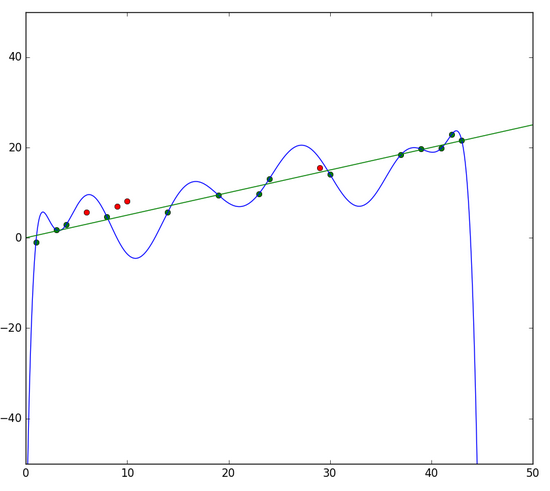
\includegraphics[scale=0.4]{./tex/regularisation/surapp.png}
    \caption{Exemple de sur-apprentissage (bleu) et d'apprentissage optimal (vert)}
    \label{surapp}
\end{figure}

\noindent Pour expliquer cette problématique, observons la Figure \ref{surapp}. Nous pouvons observer des points verts représentant les données du jeu d'apprentissage et des points rouges, les données inconnues qui doivent être prédites par le modèle. La courbe bleu et la courbe verte présentent deux fonctions apprises par deux modèles. On peut apercevoir que la courbe bleue passe par l'ensemble des points verts alors que la courbe verte possède une moins bonne performance. On peut donc naïvement dire que la courbe bleue a mieux appris. C'est vrai dans l'absolu: la courbe bleue a mieux appris le jeu de données d'apprentissage mais en plus d'apprendre le comportement général des données, elle a appris son bruit, ce qui lui donne son comportement oscillant et "imprévisible". Le fait d'apprendre le bruit est appelé \textit{sur-apprentissage} et est désastreux pour le modèle qui perd ainsi sa capacité de généralisation. Au contraire, la courbe verte n'apprend pas le bruit des données. Elle apprend moins les données d'apprentissage mais conserve sa capacité de généralisation. L'idéal est donc de trouver un compromis entre apprentissage du jeu de données et capacité de généralisation: ceci est appelé \textit{compromis biais-variance}.\\

\noindent Une explication graphique est visible sur la Figure \ref{compbv}. Le biais représente l'erreur réalisée sur l'apprentissage des données. Ainsi, un biais très faible sous-entend un sur-apprentissage car le bruit aura été appris. Au contraire, la variance représente l'importance des variations de la fonction hypothèse approximée, i.e la sensibilité du modèle aux variations des données et donc au bruit. De ce fait, plus la variance est élevée, plus le modèle perd en généralisation et devient inutilisable. Et, comme observé sur la Figure \ref{surapp}, le sur-apprentissage favorise un comportement à forte variance (représenté par les oscillations). L'objectif est donc de réaliser un compromis: optimiser la diminution du biais et de la variance.\\

\noindent D'un point de vue expérimental, la notion de biais et de variance est représentée par l'erreur de prédiction réalisée sur l'ensemble d'apprentissage et de test. Ainsi, l'objectif est d'arrêter l'apprentissage lorsque la courbe de prédiction du jeu de test augmente de manière significative alors que la prédiction sur le jeu d'apprentissage tend à diminuer.\\

\begin{figure}
    \begin{tabular}{cc}
        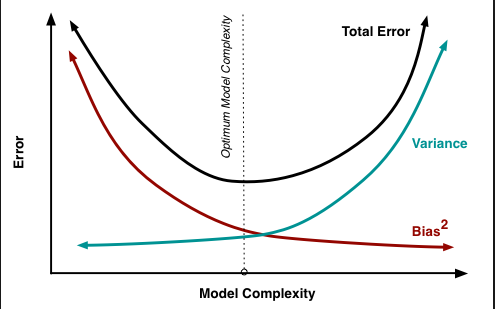
\includegraphics[scale=0.4]{./tex/regularisation/combv.png} & 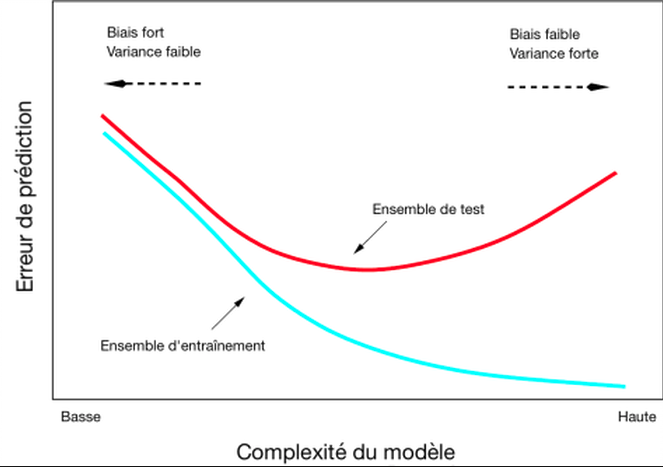
\includegraphics[scale=0.25]{./tex/regularisation/compbv2.png} \\
    \end{tabular}
        \caption{Compromis biais-variance et impact sur le modèle}
    \label{compbv}
\end{figure}

\noindent Bien sur, la problématique du sous-apprentissage existe aussi et représente un modèle trop généraliste qui n'explique pas suffisamment les données d'apprentissage qui discriminent ses prédictions. Un exemple est visible sur la Figure \ref{sousapp} où la fonction crée est bien trop "neutre". Il est évident qu'un modèle sous-entraîné possède des performances faibles.

\begin{figure}
    \centering
    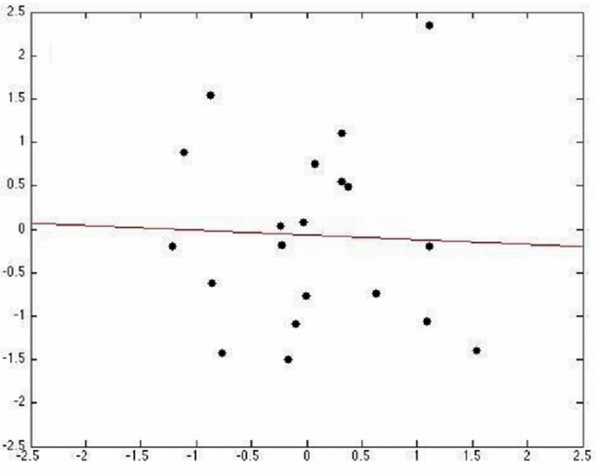
\includegraphics[scale=0.3]{./tex/regularisation/sousapp.png}
    \caption{Exemple de sous-apprentissage}
    \label{sousapp}
\end{figure}

\subsection{Limiter le sur-apprentissage}

\textbf{Important}: Cette partie est fondamentale et doit être comprise pour développer un réseau de qualité, notamment dans le cadre d'architecture très profonde que nous étudierons par la suite.\\

\subsection{Régularisation}
\label{regsec}

Les poids d'un neurone ne sont pas bornés\footnote{Dans les cas d'une architecture standard}. Cette spécificité permet une grande disparité entre les valeurs que peuvent prendre les poids d'un neurone au risque de voir certains poids \textit{exploser} alors que d'autres seraient \textit{faibles}\footnote{Cette particularité est aggravée si les données en entrée du neurone ne sont pas normalisée. Les données d'apprentissage peuvent être normalisées en entrée tout en provoquant ce phénomène en interne.}. Cette différence de valeur est très préjudiciable et favorise un comportement de sur-apprentissage où un neurone sur-réagit aux stimulations portées par les poids de haute intensité. Pour limiter l'explosion des poids, une régulation peut être imposée. \\

\noindent Cette régulation peut être associée à la fonction de coût, lui rajoutant un nouveau critère de discrimination. Ainsi, supposons la fonction de coût définie par Mean Squared Error\footnote{Voir la section \ref{fn_cout} pour plus d'informations}. Elle est définie par: $\boldsymbol{\mathcal{L}}=\frac{1}{n}\sum_{i=1}^{n}(y^{(i)}-\hat{y}^{(i)})^{2}$. Avec une régulation, nous obtenons $\boldsymbol{\mathcal{L}_{reg}}=\frac{1}{n}\sum_{i=1}^{n}(y^{(i)}-\hat{y}^{(i)})^{2}+\boldsymbol{\epsilon(\omega)}$ ou $\epsilon$ dépend uniquement des poids des neurones du réseau. Ainsi, la fonction de coût sera directement dépendant des poids des neurones et tendra à limiter leurs évolutions divergentes.\\

\subsubsection{L1-Régulation}

La première régulation est la L1-Régulation. Elle s'exprime sous la forme $\lambda|\omega|$ où $\lambda$ correspond à l'intensité associée à la régulation. Plus $\lambda$ est élevé, plus on pondère l'importance d'avoir des poids faibles. Ainsi, dans le cas de Mean Squared Error, nous obtenons $\boldsymbol{\mathcal{L}_{reg}}=\frac{1}{n}\sum_{i=1}^{n}(y^{(i)}-\hat{y}^{(i)})^{2}+\lambda|\omega|$. \\

\noindent Cette régulation est très utile dans le cas d'extraction de \textit{feature}. En effet, cette régulation tend à rendre le réseau \textit{sparse} en permettant que des poids deviennent très proches de zéro (annulant ainsi une entrée du neurone). Cette régulation favorise les entrées discriminantes et limite les entrées porteuses de bruit. Il est ainsi possible d'extraire les composantes principales du réseaux. Néanmoins, dans les faits, elle est rarement utilisée car présente de moins bons résultats que la régulation L2 (sauf dans le cas spécifique d'extraction de feature). De plus, n'étant pas quadratique, sa minimisation est difficile.

\subsubsection{L2-Régulation}
\label{l2_reg}
L2-Regulation est définie par la contrainte $\frac{1}{2}\lambda\omega^2$. La fonction de coût régulée devient donc $\boldsymbol{\mathcal{L}_{reg}}=\frac{1}{n}\sum_{i=1}^{n}(y^{(i)}-\hat{y}^{(i)})^{2}+\frac{1}{2}\lambda\omega^2$.\\

\noindent Cette régulation favorise des valeurs de poids proches en limitant les pics de valeurs. Ainsi, elle permet de faire en sorte que le neurone ne se focalise pas sur des entrées dominantes tout en délaissant les autres jugées moins pertinentes. Elle limite dons la sur-spécialisation et de ce fait, l'overfitting. Cette régulation est efficace et très utilisée aujourd'hui.

\subsubsection{ElasticNet-Régulation}

ElasticNet-Régulation est une combinaison linéaire de la Régulation L1 et L2. Elle s'exprime sous la forme $\lambda_1|\omega|+\frac{1}{2}\lambda_2\omega^2$ où $\lambda_1$ et $\lambda_2$ définissent l'importance de cette régulation dans le calcul de la performance du modèle et la pondération entre les deux régulations (comportement équilibré ou pondération d'une des deux régulations). Ainsi, la fonction de coût est dorénavant définie par la relation suivant:  $\boldsymbol{\mathcal{L}_{reg}}=\frac{1}{n}\sum_{i=1}^{n}(y^{(i)}-\hat{y}^{(i)})^{2}+\lambda_1|\omega|+\frac{1}{2}\lambda_2\omega^2$\\

\noindent Cette régulation réunit \textit{le meilleur des deux mondes} (issus de L1 et L2) bien que moins souvent appliquée que la L2-Régulation.

\subsection{Max norm constraints}

Contrairement à la régulation L1 et L2, Max norm constraints ne s'applique pas à la fonction de coût mais directement au vecteur de poids du neurone. Alors que L1 et L2 pénalisent les poids élevés\footnote{Pénaliser augmente la fonction de coût mais il n'y a pas de contrainte directe imposée à l'intégralité du réseau. Ainsi, L1/L2 favoriseront la limitation des poids les plus élevées en priorité alors que Max norm constraints les corrigera tous sans distinction}, Max norm constraints agit directement sur ces derniers. Ainsi, chaque vecteur de poids doit respecter la condition $||\omega||_2 < cnst$ ou cnst de petite taille (2,3 voire 4 par exemple). Si l'égalité n'est pas respectée, l'intégralité des poids est normalisée\footnote{Ce n'est pas la normalisation au sens statistiques !} afin de respecter la condition.\\

\noindent Cette régulatisation est particulièrement performante associée avec le \textit{DropOut}\footnote{Voir http://www.cs.toronto.edu/~rsalakhu/papers/srivastava14a.pdf, partie 5.1} mais présente la difficulté de paramétrage du seuil (cnst) qui est un hyperparamètres. Sa détermination se fait de manière empirique et expérimentale, ce qui peut rendre sa recherche délicate.

\subsection{DropOut}

Contrairement à la régulation qui agit sur les neurones de manière isolée, le DropOut\cite{dropout_deep} est une approche de régulation d'architecture, i.e une approche qui influence l'interaction entre neurones. Le DropOut sélectionne aléatoirement (selon une probabilité $\rho$) des neurones du réseau et leur impose une activation\footnote{L'activation correspond à la somme pondérée des entrées} nulle. La sélection des neurones inactifs est renouvelée à chaque donnée d'apprentissage. Lors de l'utilisation du réseau hors apprentissage, chaque sorties des neurones concernées par le DropOut sont multipliées par $\rho$ et toutes sont actives. Un exemple est visible sur la Figure \ref{dropoutdropco}.\\

\noindent Cette méthode permet de limiter l'inter-dépendance (Voir Section \ref{dead_relu}) entre les neurones et favorise la création d'un réseau éparse. L'apprentissage du modèle est ainsi plus robuste, plus rapide et moins soumis aux problématiques associées au gradient. Le DropOut est souvent exploité en plus d'une \textit{Régulation} des poids bien que son comportement soit comparable à la régulation L2. Une valeur standard pour $\rho$ est 0.5. Cette approche est souvent employée pour les réseaux Full-Connected mais peut être appliquée à d'autres architecture notamment les réseaux convolutifs. Néanmoins, l'efficacité de son utilisation sur des couches convolutives est sujet à débat.\\

\noindent \textbf{Important}: DropOut est souvent utilisé avec des fonctions d'activation f tel f(0)=0. En effet, le DropOut ne force pas la sortie à 0 mais son activation. Ainsi, si une fonction d'activation n'est pas nulle en 0, le neurone ne sera pas (complètement) inactif bien que son comportement soit constant. De plus, le biais est indépendant de l'activation et n'est pas soumis au DropOut.

\begin{figure}
\centering
        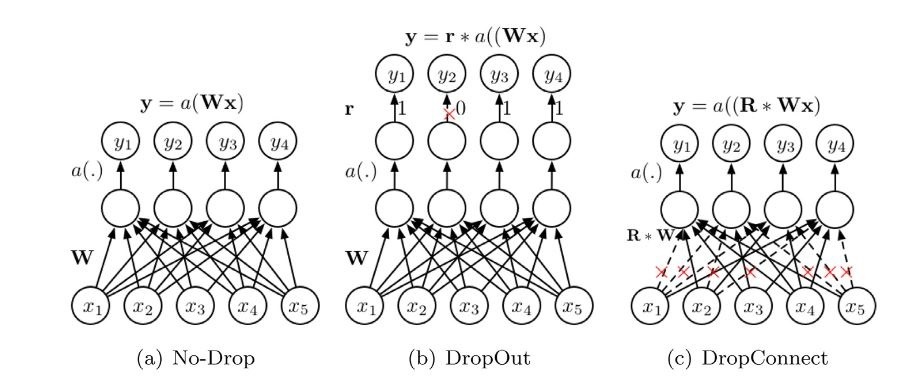
\includegraphics[scale=0.4]{./tex/regularisation/droppic.png}
    \caption{Comparaison d'un réseau sous DropOut et DropConnect}
    \label{dropoutdropco}
\end{figure}

\begin{figure}
   \centering
         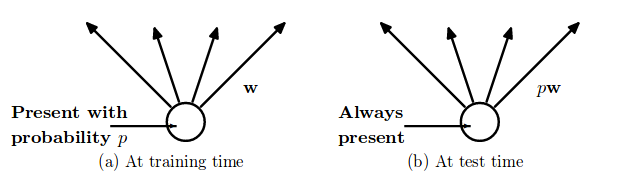
\includegraphics[scale=0.4]{./tex/regularisation/drop2.png} \\
    \caption{Relation des poids après DropOut}
    \label{dropout_fig}
\end{figure}

\subsection{DropConnect}

\noindent DropConnect\cite{dropconnect_deep} est une généralisation de DropOut. Au lieu de supprimer l'activité d'un neurone en bloquant son activation, cette méthode annule les poids d'entrée du neurone de manière indépendante selon une probabilité $\rho$. Ainsi, un neurone peut voir son activation éteinte (comparable à DropOut) ou juste partiellement. Un exemple de DropConnect est visible sur la Figure \ref{dropoutdropco}. Cette méthode est moins utilisée que DropOut et ses résultats plus rares. Il n'est pas aisé de déterminer quelle approche est la plus performante objectivement mais le DropConnect offre plus de souplesse et de configurations possibles.

\subsection{DisturbLabel}

\noindent DisturbLabel\cite{disturblabel} est une méthode de régularisation qui exploite l'approche par \textit{bruitage}. L'idée derrière cette méthode est de modifier aléatoirement le label d'une donnée d'apprentissage dans chaque minibatch d'apprentissage. On suppose une problématique multi-classe bien qu'il soit possible de généraliser à une problématique multi-label.\\

\noindent Ainsi, DisturbLabel rajoute une étape de sampling supplémentaire qui génère, pour chaque couple de donnée $(x_D,y_C)$, un vecteur label $\Hat{y}=[\Hat{y}_1,..., \Hat{y}_C]$ (avec C, nombre de label) issu d'une loi Multinouilli (Bernouilli généralisée) $P(\alpha)$ tel que:
\begin{align*}
    \Hat{c} &\sim P(\alpha)\\
    \Hat{y}_c &= 1\\
    \Hat{y}_i &= 0, \ \forall i \neq \Hat{c}\\
\end{align*}

\noindent De même, $P(\alpha)$ est définie par $p_c=1-\frac{C-1}{C}$ et $p_i=\frac{1}{C}*\alpha$ pour tout $i \neq c$ et c, indice du label valide. $\alpha$ est le \textit{taux de bruitage}. Si $\alpha=0$, il n'y a pas de bruitage. Si $\alpha \rightarrow 100\%$, alors la labellisation du jeu d'apprentissage est aléatoire. Il est donc nécessaire de garder un $\alpha$ de faible valeur.

\subsection{Dense-Sparse-Dense training}

Le Dense-Sparse-Dense\cite{dsd_deep} training est une méthode comparable à une variante du DropOut/DropConnect. Cette méthode cherche à proposer une méthode d'apprentissage plus efficace dans le cadre de réseaux très profonds. L'idée soutenue par cette méthode est qu'un réseau très profond est capable d'acquérir une compréhension plus profonde d'un phénomène mais plus enclin à en apprendre le bruit et le comportement instable. Leur postulat est que le bruit est porté par les poids faibles des neurones. Ainsi, l'objectif est d'être capable d'isoler les poids d'importance qui propagent une information fiable et les poids qui propagent le bruit. Pour cela, cette méthode (Figure \ref{dsd_fig}) se découpe en 3 phases:

\begin{enumerate}
    \item \textbf{Initial Dense Phase}: L'apprentissage du réseau est fait normalement sans contrainte particulière. Les méthodes de régulations (et autres) peuvent être exploitées durant cette phase. L'objectif de cette phase n'est pas "d'apprendre" mais de détecter les poids influents et non influents (en fonction de leurs valeurs absolues).

    \item \textbf{Sparse Phase}: Durant cette phase, les poids sont classées par couche selon leurs valeurs. Seuls les $\lambda$\% plus élevés sont conservés intacts, les autres devenant nuls. $\lambda$ est un hyperparamètre à déterminer (il est conseillé de prendre une valeur entre 25\% et 50\% comme valeur par défaut). Le réseau devient alors éparse, permettant d'obtenir un réseau plus robuste et plus économe. Il est empiriquement montré qu'un réseau éparse tend à avoir des résultats équivalents voir meilleurs qu'un réseau dense car ce dernier est plus sensible aux problématiques d'apprentissage. Un apprentissage du réseau est réalisé avec cette architecture.

    \item  \textbf{Final Dense Phase}: Durant cette phase, les connexions coupées sont restaurées. Les poids restaurés sont initiés à 0 et le pas d'apprentissage du gradient faible (1/10 du pas initial). En effet, le réseau actuel présente une stabilité et une convergence correcte. Il n'est donc pas souhaitable de "bouleverser" son architecture mais juste de favoriser sa performance en finalisant son comportement dans ses détails d'apprentissage. Le réseau peut ainsi converger vers un meilleur minimum local voire "en sortir" vers un autre selon le cas.

    \item \textbf{Répétition}: Ce cycle (3 phases) peut être répété afin de favoriser une meilleure convergence.
\end{enumerate}

\begin{figure}
    \centering
    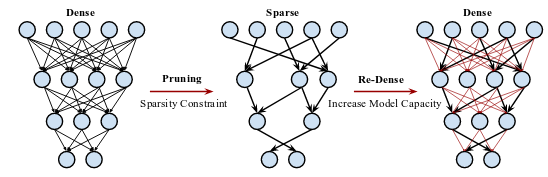
\includegraphics[scale=0.4]{./tex/regularisation/dsd.png}
    \caption{Dense-Sparse-Dense Routine}
    \label{dsd_fig}
\end{figure}

\subsection{Batch Normalization}

Batch Normalization\cite{batchnorm_deep} est une méthode qui vise à augmenter la robustesse du modèle en favorisant sa capacité de généralisation. Supposons un jeu de données d'image de chiens blancs, si une image d'un chien noir apparaît lors de la prédiction, il est évident que le réseau ne fonctionnera pas car la distribution des données d'apprentissage et de prédiction ne correspondent pas. Néanmoins, le comportement des données peut être similaire et donc, la fonction obtenue sur les chiens blancs pourraient être effective. Batch Normalization permet d'aligner les distributions et de limiter cette problématique. Un exemple illustratif est visible sur la Figure \ref{bnex}. La justification de performance de cette approche est très mathématique et repose sur un socle solide de Statistiques. Nous ne l'étudierons pas dans cette introduction.\\

\noindent L'idée de Batch Normalization est de généraliser la normalisation des données à travers le réseau de neurones. La méthode est comparable à une normalisation standard mais présente des spécificités associées à la présence d'un minibatch qui représente un sous-ensemble du jeu d'apprentissage (qui plus est, variable). La normalisation réalisée est visible sur la Figure \ref{batchnorm_fig}. Veuillez vous référer à la publication associée\cite{batchnorm_deep} pour plus de détails mathématiques sur son fonctionnement.  \\

\noindent De plus, cette méthode permet de mieux isoler les couches entre elles, limitant l'inter-dépendance, permet d'utiliser un pas d'apprentissage plus important car les données internes au réseau sont normalisées (ce qui limite les valeurs extrêmes et donc les valeurs du gradient) et possède une action de régulation. L'utiliser avec DropOut (ou équivalent) est efficace bien qu'il soit préférable d'utiliser une probabilité plus faible d'éteindre un neurone dans cette configuration. Un gain de vitesse est aussi observé du fait de la limitation des valeurs des données, ce qui favorise une implémentation optimisée.\\

\noindent De même que le DropOut, Batch Normalization fait partie des améliorations majeures proposées dans le cadre du développement d'un réseau de neurones et son utilisation est quasi-récurrente à tout réseau d'ampleur.

\begin{figure}
    \centering
    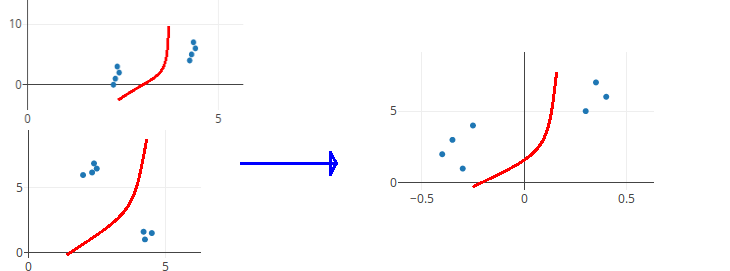
\includegraphics[scale=0.4]{./tex/regularisation/bn1.png}
    \caption{Non-alignement des distributions}
    \label{bnex}
\end{figure}

\begin{figure}
    \centering
 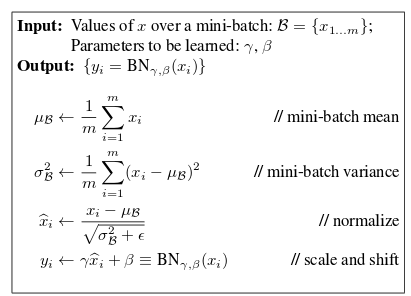
\includegraphics[scale=0.4]{./tex/regularisation/batchnorm.png}
    \caption{Normalisation par Batch Normalization}
    \label{batchnorm_fig}
\end{figure}

\subsection{Critère d'arrêt de l'apprentissage}
Pour réaliser un bon apprentissage, il est nécessaire de considérer le \textit{compromis biais-variance} afin de limiter le sur-apprentissage. Bien que la problématique soit facilement assimilable, s'en prémunir reste difficile.\\

\noindent Une bonne pratique repose sur l'utilisation d'architectures de régulation qui tend à limiter le phénomène de sur-apprentissage\footnote{Phénomène présent lorsque la courbe de biais diminue et la courbe de variance augmente}. Bien que fonctionnelles, ces architectures ne garantissent pas un apprentissage contrôlé. Une approche complémentaire est donc de savoir \textbf{quand} arrêter l'apprentissage afin d'obtenir le meilleur état du modèle. Dans le cas idéal, l'arrêt se situe à l'intersection de la courbe de biais et de variance. Mais comment savoir si on se situe dans un intervalle proche de ce point de référence ?\\

\noindent La courbe de biais est associée aux erreurs de prédiction sur les données d'apprentissage alors que pour la courbe de variance, ce sont les erreurs de prédiction sur les données de validation (Figure \ref{compbv}). La courbe de biais décroît logiquement durant l'apprentissage jusqu'à atteindre une valeur asymptotique caractérisée par un résidu de bruit. Au contraire, la courbe de variance va décroître progressivement avant de croître lorsque le modèle commence à perdre sa capacité de généralisation. L'objectif étant d'assurer la meilleure performance prédictive tout en ayant une forte capacité d'abstraction, se concentrer sur le comportement de la courbe de variance semble prioritaire. Il est ainsi nécessaire de détecter le minimum global de cette fonction alors que la courbe de biais ne présente qu'une importance secondaire. Il serait même dangereux de se concentrer sur la courbe d'apprentissage car une erreur très faible d'apprentissage est souvent associée à un sur-apprentissage important.\\

\noindent Sur la Figure \ref{compbv}, la courbe de variance est idéalisée. Dans les faits, elle présente souvent du bruits et des oscillations locales qui rendent son étude délicate (Figure \ref{early_courbe}). La problématique du minimum local est au coeur du problème et il n'existe pas de solution idéale actuellement pour garantir un arrêt optimal de l'apprentissage du modèle. Néanmoins, plusieurs approches existent et présentent des résultats satisfaisants. Ces fonctions de régulation sont appelées \textbf{Early Stopping}.

\begin{figure}
    \begin{tabular}{cc}
       a) 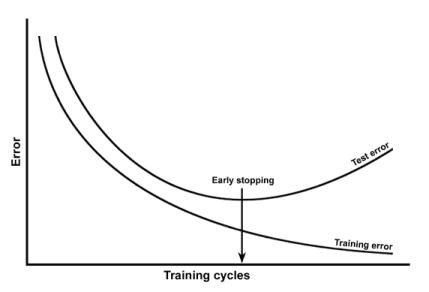
\includegraphics[scale=0.9]{./tex/regularisation/valid_ideal.png} &
         b) 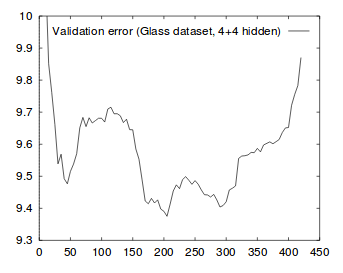
\includegraphics[scale=0.4]{./tex/regularisation/val_reel.png}\\
    \end{tabular}
    \caption{a) Early Stop théorique b) Comportement-type de l'erreur de validation en situation réelle}
    \label{early_courbe}
\end{figure}

\subsubsection{Early Stopping}
Les méthodes \textit{Early Stopping} repose sur la valeur de l'erreur de validation. De ce fait, nous définissons $E_{opt}(t)$, l'erreur de validation la plus faible jusqu'à l'instant t, définie par: $E_{opt}(t)=\underset{t' \leq t}{min}(E_{va}(t'))$ avec $E_{va}$, erreur de validation.

\paragraph{Generalization Loss ($GL_\alpha$)}
La première méthode, nommée Generalization Loss ($GL_\alpha$)\cite{earlystop}, repose sur l'augmentation relative de l'erreur à l'instant t par rapport à $E_{opt}(t)$. Ainsi, si l'augmentation est supérieure à une valeur donnée, l'apprentissage est stoppé. Ce critère examine la tendance absolue de l'évolution de l'erreur de validation et néglige la tendance évolutive locale.\\

\noindent Pour formaliser mathématiquement ce comportement, nous définissons l'erreur (en pourcentage) par:
$$GL(t)=100*(\frac{E_{va}(t)}{E_{opt}(t)}-1)$$
$$Stop: \ GL(t) > \alpha$$

\noindent Cette approche est peu efficace pour lutter contre les minimum locaux. Exploiter ce critère d'arrêt aura tendance à stopper l'apprentissage lorsqu'un minimum local aura été observé. Bien qu'efficace en cas de comportement convexe de la fonction d'erreur, elle est peu performante dans le cas contraire. Expérimentalement, ce critère limitera la capacité d'exploration du réseau durant sa phase d'apprentissage et peut favoriser un arrêt prématuré.

\paragraph{Quotient of Generalization Loss and Progress ($PQ_{alpha}$)}
La méthode $GL_{\alpha}$ ignore le comportement du modèle sur les données d'apprentissage. En ignorant ces informations, ce critère n'a pas connaissance de la situation d'apprentissage du réseau. La variation de l'erreur d'apprentissage peut donc être faible ou élevée sans qu'elle n'ait d'impact sur le critère d'arrêt. Expérimentalement, on observe que le sur-apprentissage arrive souvent lorsque l'erreur d'apprentissage décroît "lentement" après une diminution brutale en début d'apprentissage (Figure \ref{earlystop}). De même, intuitivement, il est pertinent de penser qu'une variation importante de l'erreur d'apprentissage est corrélée avec une amélioration significative du réseau ou tout du moins, une variation significative de son comportement prédictif. L'impact de cette variation sur le comportement prédictif doit être considéré avant d'imposer l'arrêt de l'apprentissage. Pour considérer cet aspect, la notion de \textit{Progress} ($P_k$)\cite{earlystop} est introduite. Elle évalue l'importance de la variation de l'erreur moyenne sur un intervalle donné par rapport à l'erreur minimale observée.\\

\noindent Supposons un intervalle de k itérations successives et $E_{tr}(t)$, erreur d'apprentissage à l'instant t alors:
$$P_k(t)=1000*(\frac{\sum_{t'=t-k+1}^tE_{tr}(t')}{k*min_{t'=t-k+1}^tE_{tr}(t')}-1)$$

\noindent Nous voulons poursuivre l'apprentissage si l'erreur d'apprentissage s'améliore significativement. De ce fait, la valeur de $P_k$ doit minorer l'expression de $GL(t)$. Pour cela, nous définissons $PQ_{\alpha}$\cite{earlystop} tel que:
$$Stop: \ \frac{GL(t)}{P_k(t)} > \alpha$$

\paragraph{Successive Generalization Error ($UP_s$)}
Les méthodes précédentes exploitent une approche absolue pour l'analyse de la tendance de la courbe d'erreur. Un procédé complémentaire serait de considérer les tendances locales de la courbe d'erreur. Pour cela, $UP_1$ observe la variation de $E_{va}$ pour un intervalle [n, n+k] donné et provoque un arrêt de l'apprentissage si la variation correspond à une augmentation de l'erreur de validation.\\

\noindent En généralisant, nous obtenons:
$$UP_1: \ stop: \ E_{va}(t) > E_{va}(t-k)$$
$$UP_s: \ stop: \ UP_{s-1} \rightarrow stop \ \cup \ E_{va}(t) > E_{va}(t-k)$$

\noindent \textbf{Remarque}: Il est important d'observer le comportement récursif de $UP_s$ où s indique le nombre de variations successives considérées.\\

\noindent Cette méthode favorise la capacité d'exploration du modèle en l'émancipant de la considération absolue de sa performance\footnote{Le critère d'arrêt se limite à observer ses évolutions locales et non absolues}. $UP_s$ est donc plus performant pour détecter le meilleur minimum local que $GL_{\alpha}$. Néanmoins, cette approche facilite le risque de divergence du modèle et peut être inefficace en cas de variations progressives.\\

\noindent Supposons $UP_{s=4}$. Si la courbe d'erreur de validation suit un cycle itératif défini par 3 hausses positives\footnote{ou moins} de l'erreur ($e_1^+, e_2^+, e_3^+$) suivie d'une diminution de l'erreur ($e_4^-$) tel que $\sum_{i=1}^4 e_i^{+-}>0$, alors le critère d'arrêt est inefficace et la fonction d'erreur divergera.\\

\noindent Ces deux familles de \textit{Early Stopping} peuvent être combinées afin d'exploiter les deux axes d'analyse de la tendance de l'erreur de validation. Il est donc possible de réaliser une combinaisons linéaire de plusieurs de ces critères et de pondérer les critères selon l'importance qu'on souhaite leur attribuer.\\

\subsubsection{Arrêt supervisé}
\noindent L'apprentissage d'un réseau de neurones est (généralement) une tâche de longue durée qui rend possible une supervision visuelle. Exploiter des outils de visualisation durant l'apprentissage est une approche à ne pas sous-estimer et souvent, présentera les meilleurs résultats.\\

\noindent Les API de Deep Learning proposent des interfaces de visualisation pour faciliter ce travail, notamment \textit{Tensorboard} associé à l'API de Google, \textit{Tensorflow}.

\begin{figure}
    \centering
    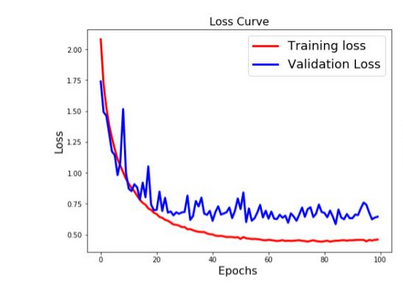
\includegraphics[scale=0.4]{./tex/regularisation/earlystop.png}\\

    On observe que la courbe d'erreur d'apprentissage est comparable à un logarithme inversé. Sur cet exemple, le sur-apprentissage ne semble pas présent.
    \caption{Exemple de courbe d'erreur d'apprentissage et de validation}
    \label{earlystop}
\end{figure}

\subsection{Data Augmentation}

Une des difficultés principales des réseaux de neurones est l'exigence d'une quantité importante de données d'apprentissage, quantité qui augmente avec la profondeur du réseau. Il n'est pas rare d'utiliser des jeux d'apprentissage contenant des millions voire des milliards d'entités, notamment dans l'étude du langage (Natural language Processing). \\

\noindent Obtenir un jeu de données est difficile, chronophage (et potentiellement cher si il doit être annoté dans le cas du traitement du langage ou de la segmentation d'image). Il est donc indispensable d'utiliser des méthodes afin, à partir d'une entité, d'en créer d'autres de manière artificielle. Il est possible de créer tout type de données de manière artificielle à partir d'une base suffisante le permettant (texte, signal 1D, 2D, ...). Chaque type de données utilise des méthodes différentes propres à son type. \\

\noindent Ainsi, dans le cas d'une image (signal 2D), plusieurs approches sont possibles:
\begin{itemize}
    \item \textbf{Variation géométrique}: Rotation, inversion, symétrie, translation
    \item \textbf{Analyse de densité de la distribution de pixels (via l'histogramme)}: contraste, filtrage, effet flou
    \item \textbf{Analyse statistiques}: Création par PCA, Création par ZCA
    \item \textbf{Signal bruité}: Ajout de bruit gaussien, bruit poivre et sel, bruit multiplicatif
    \item \textbf{Création de contenu}: Création de patterns génériques (fusionner deux photos par "collage" brut par exemple - efficace dans le cadre de la segmentation)
\end{itemize}

\noindent Il existe de nombreuses autres méthodes et ce, pour tout type de données. Un jeu d'apprentissage est de qualité si il est le plus représentatif et diversifié possible. Cette étape est donc importante car un jeu de données de qualité est une \textbf{condition nécessaire et primordiale} pour un apprentissage de qualité. \textbf{Peu importe la qualité du modèle, si les données sont de médiocre qualité, l'apprentissage sera mauvais}.

\subsection{Complexité de l'architecture et mémoire}
\label{deepcompsec}
Le Deep Learning a connu un regain de popularité grâce à l'évolution matérielle qui, dorénavant, supporte ce type d'architecture. Néanmoins, les réseaux très profonds demandent des ressources très importantes qui ne sont pas à la portée de tous (particulier comme professionnel). Un modèle complexe demande un temps très important d'apprentissage et le temps de prédiction peut être trop important pour supporter les conditions du temps réel (analyse vidéo ou vocale par exemple). De plus, une contrainte importante de mémoire dédiée peut avoir lieu dans le cadre de structures limitées telle que l'embarqué. Il est donc important de proposer des approches pour optimiser l'architecture d'un réseau. En effet, il est \textbf{important} de ne pas associer la profondeur d'un réseau avec une preuve de qualité. Un réseau très profond peut être moins performant qu'un réseau plus simple bien que sa capacité d'abstraction soit plus forte. Les difficultés d'apprentissage sont un facteur déterminant et il est souvent plus aisé d'optimiser un réseau plus petit qu'affronter la complexité d'un modèle théoriquement plus performant mais plus délicat à développer.\\

\noindent Pour cela, différentes méthodes de simplification de modèle existe, notamment \textit{Deep Compression}\cite{deepcomp_deep}. Cette méthode reprend l'idée de suppression des poids faibles issue du \textit{Dense-Sparse-Dense training}. L'objectif de cette compression est de limiter le temps d'apprentissage du modèle (de ce fait, sa complexité) et la mémoire nécessaire pour le stocker. L'approche \textit{Sparse} limite la complexité du modèle et l'optimisation de la mémoire est réalisée en deux étapes. Nous ne détaillerons pas ces deux étapes en détails, pour cela, veuillez vous référer au papier associé. \textit{Deep Compression} se déroule ainsi:

\begin{enumerate}
    \item \textbf{Sparse}: Suppression des poids faibles du réseau
    \item \textbf{Optimisation des poids et des gradients}: Afin de limiter le stockage de valeurs, une approche par clustering (Kmeans) est réalisée afin de réaliser des clusters de poids semblables. Ces poids seront donc, dans un premier temps, représentés par la valeur du centroïde\footnote{L'initialisation du Kmeans est une étape importante à étudier et à ne pas négliger} du cluster (souvent associé au barycentre). Les matrices du réseau seront donc associées à des index pointant sur la valeur du centroïde concerné. Les gradients de chacun des poids sont calculés, additionnés entre eux selon la répartition de leurs poids associés parmi les clusters définis précédemment et les gradients de chaque cluster multipliés par le pas d'apprentissage. La valeur des centroïdes sera alors mise à jour par la soustraction de la valeur du centroïde avec celle du gradient du cluster associé.
    \item \textbf{Application du codage de Huffman}: Afin de limiter le poids des matrices de poids (ou d'index), on applique un codage de Huffman. le codage de Huffman permet de réaliser une compression de données sans perte.
\end{enumerate}

\noindent Un exemple illustratif de la phase 2 est visible sur la Figure \ref{deepcomp}. Il existe d'autres méthodes bien que ce genre d'approche soit, aujourd'hui encore, expérimental et peu appliqué dans l'industrie. Cependant, il est fort probable qu'elles se développeront dans le futur du fait de la complexité grandissante des modèles crées.

\begin{figure}
    \centering
    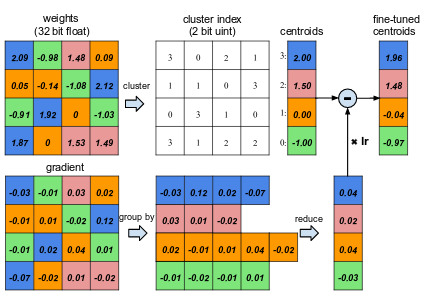
\includegraphics[scale=0.4]{./tex/regularisation/deepcomp.png}
    \caption{Optimisation réalisée sur les matrices de poids par Deep Compression}
    \label{deepcomp}
\end{figure}

\subsection{Transfer Learning}
\textbf{Important}: Cette partie va supposer que vous avez une connaissance générale des \textbf{réseaux convolutifs}. Si non, veuillez vous référer à la Section \ref{conv_sec}. On supposera le cas d'un réseau convolutif pour illustrer cette partie.\\

\noindent L'une des grandes problématiques du Deep learning est son temps d'apprentissage. Même sur des modèles jugés simples, l'apprentissage demande des ressources matérielles importantes et ce, pour une longue durée. L'objectif du \textit{Transfer Learning} est d'étudier les capacités d'un apprentissage à se généraliser à différents problèmes. Par exemple, un réseau convolutif ayant appris sur un jeu de d'images spécifiques peut-il être réutilisé sur un autre jeu d'images ? Si oui, dans quelle mesure ? Cette problématique est l'un des sujets de recherche parmi les plus actifs avec des retombés applicatives très importantes. Cette fonctionnalité est très importante dans le cas d'analyse d'image ou de texte (projection vectorielle de mots ou Words Embeddings)\\

\noindent Dans le cadre du Deep Learning, l'ensemble des approches de Transfer Learning sont exploitées. Chaque approche possède ses propres familles de réseaux et spécificités.

\paragraph{Inductive Transfer - Parameter Transfer}

\noindent La méthode \textit{Parameter Transfer} est particulièrement populaire, notamment pour les réseaux convolutifs. La problématique sous-jacente à cette approche revient à définir si des poids d'un réseau peuvent être utilisés par un autre réseau pour son apprentissage. \\

\noindent Classiquement, les couches de convolution d'un réseaux convolutifs peuvent être interprétées comme des extracteurs d'attributs d'une image, i.e extraire l'information utile et discriminante. Ces attributs sont alors différenciables par un réseau Feed-Forward standard. Il est évident que le modèle Feed-Forward est entraîné à discriminer les entités selon le jeu de données d'apprentissage. Il n'est pas pas ou très peu ré-utilisable dans d'autres contextes\footnote{Un réseau qui a appris à discriminer un chat ne pourra discriminer une voiture}. Mais il est logique de se demander si extraire des attributs d'une image est généralisable ou spécialisé d'un jeu de données particulier.\\

\noindent Les couches de convolution agissent comme des couches d'abstraction de l'image. Les premières couches isolent grossièrement les attributs de l'image et les couches finales, analysent ces attributs de manière plus spécifique et détaillée. Ainsi, plus le modèle est profond, plus sa représentation finale des données aura un haut niveau d'abstraction spécifique aux données d'apprentissage et ses couches finales seront très affiliées au données d'apprentissage (couches généralistes $\underset{\infty}{\longrightarrow}$ couches spécialisées). Les couches de convolution peuvent ainsi être généralisées car l'extraction d'attribut d'une image n'est pas nécessairement associée à une catégorie de données spécifiques (notamment dans les premières couches de convolution) car très généralistes.\\

\noindent Pour illustrer, supposons que nous souhaitons différencier deux voitures. Tout d'abord, nous considérerons la taille, la couleur dominante par exemple, i.e le comportement des premières couches de convolution alors que par la suite, nous étudierons la forme des jantes ou des rétroviseurs. Analyser la taille et la couleur peut être utile pour discriminer deux chats mais analyser la forme des jantes est peu efficace... Ainsi, le \textit{Transfer Learning} permet de limiter le "gaspillage" d'apprentissage mais des précautions doivent être prises selon les spécificités du modèle qu'on souhaite réutiliser et les nouvelles données d'apprentissage.\\

\noindent Aujourd'hui, il existe des jeux de données variées et de grande qualité (ImageNet, Cifar,...). Ces jeux de données sont très diversifiées (avec des centaines voire des milliers de classes). Ils sont donc généralistes\footnote{Si on cherche à étudier des entités d'un même domaine d'activité. Etudier des images de microbiologie à partir d'un modèle ayant appris sur des images issues d'expériences en astrophysique sera difficile quelque soit la diversité de l'apprentissage sur son domaine.}. De nombreux modèles pré-entraînés sur ces données sont en open-source et facilitent grandement le temps d'apprentissage.\\

\noindent Trois possibilités s'offrent à l'utilisateur:
\begin{enumerate}
    \item \textbf{Extracteur figé}: Dans cette configuration, on juge que les couches exportées sont fiables et finalisées. On figera donc leurs poids en bloquant les modifications par rétropropagation. Dans le cas d'une extraction de couches de convolution, la sortie obtenue par ces couches est appelée \textbf{CNN codes}.

    \item \textbf{Extracteur variable}: Dans cette configuration, les couches exportées ne sont pas figées et continuent d'apprendre durant la spécialisation du réseau sur le nouveau jeu de données. Le \textit{Transfer learning} agit donc comme une initialisation des poids du réseau (bien plus pertinent que l'aléatoire).

    \item \textbf{Modèle pré-entrainé}: Bien qu'il y ait des modèles puissants réalisés (en général) par des universités et/ou des entreprises privées, une communauté importante s'est développée pour favoriser la création de modèles déjà pré-entrainés. Ces modèles sont souvent moins "performants" que les modèles réputés et reconnus du fait de la différence de ressources et de temps d'apprentissage du réseau. Néanmoins, il est possible de trouver des réseaux ayant appris sur un jeu de données plus semblables au votre que les modèles standards ayant appris sur des données généralistes. Ces modèles offrent donc une alternative très performante notamment dans le cadre de l'initialisation de poids. On parlera alors de \textit{Fine-Tuning}.

\end{enumerate}
\noindent Le choix de l'approche à choisir dépend essentiellement de la taille du nouveau jeu de données et de leurs différences.
\begin{itemize}
    \item \textbf{Nouveau jeu de données similaire au jeu d'apprentissage et de petite taille}: A cause de la petite taille du nouveau jeu de données, le risque de sur-apprentissage est important. Comme le jeu de données d'apprentissage et proche du nouveau jeu de données, il est préférable de figer les couches de convolution et d'apprendre uniquement un nouveau modèle Feed-Forward pour la classification.

    \item \textbf{Nouveau jeu de données similaire au jeu d'apprentissage et de grande taille}: Grâce à la grande taille du jeu de données, il est possible de mettre à jour les poids des couches transférées car le risque de sur-apprentissage est plus faible. Le Transfer Learning joue un rôle d'initialisation des poids dans cette configuration et l'apprentissage spécialisera votre modèle.

    \item \textbf{Nouveau jeu de données de petite taille et très différent du jeu d'apprentissage}: Cette situation est peu  propice au Transfer Learning. En effet, le jeu d'apprentissage de petite taille ne permet pas un apprentissage des poids performant, il est donc nécessaire de limiter la mise à jour des poids des couches transférées. Cependant, la différence importante entre les deux jeux de données présente un risque de mauvaise performance due à la sur-spécialisation de ces couches. Afin de trouver un compromis, il est intéressant de ne pas garder \textbf{l'intégralité} des couches de convolutions mais d'en garder un sous-ensemble en supprimant les dernières couches qui présentent la spécialisation la plus forte. Ainsi, nous transférons que les couches les plus généralistes qu'on peut supposer performantes pour différencier des images de catégories différentes. Bien sûr, un nouveau modèle Feed-Forward doit être appris intégralement.

    \item \textbf{Nouveau jeu de données différent du jeu d'apprentissage et de grande taille}: Dans cette configuration, la grande taille du jeu de données permet un apprentissage. Néanmoins, la différence entre les deux jeux posent problème quant à la quantité des couches à transférer. Il est souvent préférable, grâce à la capacité d'apprentissage du nouveau jeu de données, d'utiliser un réseau pré-entrainé (autres que les modèles standards) qui a appris sur des données comparable aux votres afin d'initialiser les poids et d'utiliser vos données pour le spécialiser en mettant à jour les couches transférées. Un nouveau modèle Feed-Forward doit être appris.
\end{itemize}

\noindent \textbf{Important}: Le modèle Feed-Forward n'est pas impératif. En effet, d'autres algorithmes d'apprentissage automatique peuvent être utilisés notamment le SVM ou le XGboost. Néanmoins, les réseaux de neurones présentent une bonne efficacité et permettent une implémentation plus aisée en permettant la réalisation d'un modèle qui limite les dépendances de concepts.\\

\noindent Il est très difficile de considérer l'ensemble des caractéristiques d'un phénomène, c'est pourquoi la capacité de généralisation d'un modèle de \textit{Machine Learning} est très importante. Il n'est pas capital de représenter l'intégralité des hypothèses possibles\footnote{C'est d'ailleurs un travail irréalisable} mais il est nécessaire de survoler l'ensemble des grandes possibilités de représentation. Plus ce travail de diversité sera fait, plus le jeu de données sera de qualité. Il est donc évident qu'un jeu de données de grande taille aura tendance à être de meilleure qualité. Néanmoins, ce n'est pas une condition suffisante !

\paragraph{Transductive Transfer - Domain Adaptation - A FAIRE}
%https://arxiv.org/pdf/1802.03601.pdf
\subsection{Réseaux de neurones et méthodes d'Ensemble - A FAIRE}
\subsubsection{Bagging - A FAIRE}
%http://cs231n.github.io/neural-networks-3/#ensemble
\subsubsection{Boosting - A FAIRE}

\newpage

%% Convolution Network.
\section{Réseaux convolutifs}
\label{convsecmain}
\textbf{Important}: Tout ce qui a été vu précédemment s'applique à la spécificité des réseaux convolutifs.
\subsection{Généralités}
Les réseaux convolutifs constituent l'une des grandes familles d'architecture associées aux réseaux de neurones. Popularisés par Yann Lecun en 2012, ces réseaux ont montré des résultats remarquables pour l'analyse de données structurées telles que les images (mais aussi les signaux ou textes). Mais pourquoi cette architecture est préférable à un modèle Feed-Forward (Perceptron Multicouche) standard ?\\

\noindent Supposons une image de petite taille soit 15*15 par exemple. L'image est codée en RGB (images couleurs). Ainsi, l'image possède 15*15*3 valeurs distinctes correspondant à ses pixels. Dans le cas d'un modèle Feed-Forward, les neurones de la couche d'entrée devront avoir une entrée (et donc un poids) associée à chacune des valeurs de l'image soit 15*15*3=675 entrées. Bien que ça puisse impressionner, les capacités de calculs des technologies d'aujourd'hui peuvent le supporter\footnote{Bien sûr, il ne doit pas y avoir trop de couches cachées...}. Considérons une image de taille un peu plus standard soit 500*500. On obtient donc 500*500*3=750*$10^3$ poids par neurones de la couche d'entrée. Il est évident que le nombre d'entrées est bien trop important et rendrait l'apprentissage irréalisable. De même, le risque de sur-apprentissage est très important. De ce fait, les modèles Feed-Forward classique ne \textbf{peuvent pas se mettre à l'échelle}.\\

\noindent Les couches de convolution permettent d'extraire l'information d'une image et d'en réaliser une représentation à un plus haut niveau d'abstraction. Ces couches présentent deux avantages notables. Tout d'abord, elles permettent de représenter le contenu utile d'une image dans une dimension plus faible\footnote{Après traitement d'une couche de pooling} que l'image d'origine\footnote{On peut comparer ce procédé à un pré-traitement des données}, ce qui permettrait à un modèle Feed-Forward d'apprendre dessus. Dans un second temps, les couches de convolution réalisent le travail d'extraction d'information réalisée traditionnellement par des méthodes-tiers comme HoG par exemple et ce, avec une capacité d'apprentissage. Alors que les méthodes-tiers sont des méthodes figées et généralistes, les couches de convolution se spécialisent dans la discrimination des images de sa base d'apprentissage. Ainsi, elles sont souvent plus efficaces et mieux optimisées\footnote{Il a été montré qu'elles offrent une capacité de discrimination assez généraliste dans les couches de bas niveau malgré tout}. Une illustration est visible sur la Figure \ref{absconvpro}\\

\begin{figure}
    \centering
    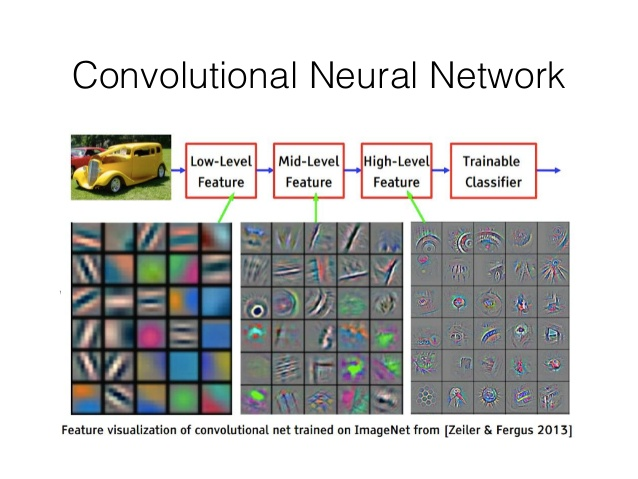
\includegraphics[scale=0.45]{./tex/convolution-network/cnn/convabs.jpg}
    \caption{Relation entre l'abstraction d'un réseau convolutif et sa profondeur}
    \label{absconvpro}
\end{figure}

\noindent Un réseau convolutif possède (dans sa version générale) l'architecture suivante:
\begin{itemize}
    \item \textbf{Couche d'Entrée}: Ceci correspond à la donnée proposée au réseau pour son apprentissage ou une prédiction. L'entrée stocke ainsi l'intégralité des valeurs de la matrice de l'image. Elle sera donc de dimension X*Y*3 dans le cas d'une image de dimension X*Y en RGB.
    \item \textbf{Couche d'extraction de caractéristiques:}\\

    Le cycle suivant est répété k fois en accord avec l'architecture du réseau.
    \begin{enumerate}

    \item \textbf{Couche de convolution}: Les couches de convolution vont extraire l'information de l'image et la représenter à un plus haut niveau d'abstraction. Il peut y avoir une ou plusieurs couches de convolution. La nature des sorties d'une couche de convolution se présente sous la forme d'une matrice de dimension x*y*z où x,y,z dépendant des paramètres de la couche\footnote{x et y inférieurs ou égaux à la dimension X et Y de l'entrée}.

    \item \textbf{Couche d'activation}: Cette couche réalise une activation selon la fonction d'activation utilisée sur les valeurs de la matrice de sortie de la couche de convolution. ReLU est la fonction la plus populaire actuellement mais d'autres peuvent être utilisées.

    \item \textbf{Couche de régulation}: Afin de limiter le sur-apprentissage, il est utile d'exploiter des couches qui aident à prévenir cette dérive de l'apprentissage. Ces couches n'ont pas de pouvoir d'extraction d'informations et se limitent à une action régulatrice. Ce type de couche modifie localement l'architecture du réseau (DropOut par exemple) ou les valeurs de sortie des couches de convolution (Batch Normalisation par exemple).

    \item \textbf{Couche de redimensionnement}: Les sorties des couches de convolution peuvent être dans un format qui ne facilite pas l'apprentissage et/ou l'optimisation de ressources matérielles. Pour limiter ce problème, un redimensionnement vers une dimension inférieure (ou supérieure) est souvent réalisé. Le redimensionnement, selon l'objectif souhaité, s'applique selon une dimension spécifique du signal donné.
    \end{enumerate}

    \item \textbf{Couche de classification (Full-Connected i.e perceptron multicouche)}: Cette couche réalise la décision du réseau à partir de l'information extraite des couches de convolution.
\end{itemize}

\noindent Il est important de noter que certaines couches possèdent des paramètres et d'autres non. En effet, les couches ReLu et Pooling appliquent une transformation fixe sur les données (donc aucun paramètre\footnote{Ceci n'est pas entièrement vrai pour les couches de Pooling car il existe des variantes qui exploitent des paramètres. De même, des variantes plus avancées de la fonction ReLU apprennent durant l'apprentissage}) alors que les couches de convolution et Full-connected "apprennent"\footnote{Par rétro-propagation} durant l'apprentissage et donc, possède des paramètres.

\subsection{Couche d'Entrée}
La couche d'Entrée est représentée par une couche de neurones où un neurone se limite à la propagation d'une valeur de la matrice de l'image observée. Chaque neurone est ainsi défini par une pondération unitaire avec une fonction d'activation linéaire. Il y a autant de neurone que de pixels dans l'image (d'où l'importance d'avoir des images de taille constante).\\

\subsection{Couche de Convolution}

\subsubsection{Nature d'une couche de convolution}

Les couches de convolution suivent une architecture Feed-Forward modifiée par la condition de connectivité locale, i.e un neurone de la couche de convolution n'est pas connecté à l'intégralité des neurones de la couche précédente (Entrée ou autre couche de convolution) mais uniquement aux neurones "les plus proches". Cette particularité diminue drastiquement le nombre de liaison des neurones, permettant leur apprentissage en temps humain. Le degrés de connectivité locale est un paramètre variable dépendant de la taille du filtre souhaité. Un filtre détermine le nombre de neurones adjacents à considérer. Plus le filtre sera grand, plus il y aura de neurones considérés. Néanmoins, bien que la taille du filtre soit variable, sa profondeur reste constante et égale à la profondeur de l'image d'entrée. Par exemple, supposons une image RGB. Sa profondeur est de 3 (channels rouge, vert et bleu). Chaque neurone possédera une connexion avec chacun de ces trois channels en accord avec les limitations du critère de connectivité locale. Il y a donc une restriction selon la largeur et la longueur de la donnée d'entrée mais pas sa profondeur. Une couche de convolution possède un filtre de dimension fixe mais peut posséder plusieurs sous-couches associées à des filtres différents (même dimension mais valeurs différentes). L'architecture d'une couche de convolution se représente donc comme un volume en 3 dimensions où la profondeur correspond au nombre de sous-couches. Une représentation graphique est visible sur la Figure \ref{conv_pic}.\\

\noindent Chaque neurone d'une même sous-couche de convolution possède un même paramétrage. Ainsi, chaque neurone possède le même biais et le même vecteur de pondération. Ils sont donc tous \textit{identiques}. Cette spécificité implique une \textit{invariance par translation} car, comme chaque neurone est identique, la localisation spatiale des pixels n'a pas d'influence sur l'analyse par un filtre donné. De ce fait, une couche de convolution limite grandement le nombre de paramètres tout en conservant les corrélations spatiales locales des images.\\

\noindent Un filtre représente le vecteur poids du neurone. Les poids des neurones ne sont pas identiques pour chaque channel. Ainsi, dans le cas d'une image RGB, un filtre possédera 3 sous-filtres qui seront appliqués sur chacun des channels de manière indépendantes. Les 3 résultats obtenus par les sous-filtres seront unis lors du calcul de la convolution. Dans la configuration standard, on considère souvent un biais nul et une fonction d'activation identité.\\

\noindent Du fait de l'utilisation d'une architecture de neurones, l'apprentissage des filtres se fait par rétro-propagation. Grâce à la connectivité locale du réseau et de l'unicité des pondération par filtre, le nombre de paramètres à apprendre est drastiquement diminué et permet au réseau d'apprendre en temps humain.

\begin{figure}
    \centering
    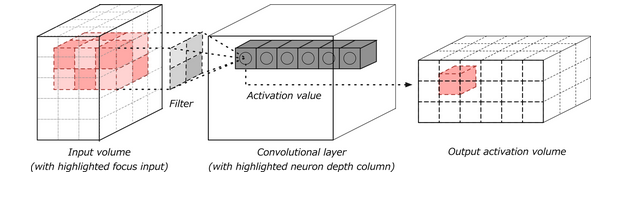
\includegraphics[scale=0.4]{./tex/convolution-network/cnn/conv_fig.png}
    \caption{Architecture d'une couche de convolution}
    \label{conv_pic}
\end{figure}

\subsubsection{Interprétation graphique}
En vulgarisant, une convolution est une opération mathématique qui décrit une règle sur comment unir deux données. Une convolution prend ainsi une entrée, applique un kernel et réalise une \textit{feature map} en sortie.\\

\noindent Dans le cadre d'une couche de convolution, la convolution est réalisée par un produit scalaire entre un filtre (kernel) et l'entrée. Un exemple est visible sur la Figure \ref{conv_fil}. Le filtre est de dimension inférieure à l'entrée (dans le cadre d'une image, inférieure à hauteur*longueur) mais de profondeur égale à la profondeur de l'image (nombre de channels d'entrée). Un filtre se comporte comme une \textit{fenêtre glissante} afin de parcourir l'intégralité de la données d'entrée. La matrice de sortie obtenue est appelée \textit{feature map}. Il y a autant de \textit{feature map} que de filtre ainsi, si il y a 4 filtres appliquées sur la donnée d'entrée, il y aura 4 \textit{feature map} en sortie.\\

\noindent La \textit{fenêtre glissante} est associée à un hyperparamètre appelé \textbf{stride}. En effet, il est possible de définir les intervalles de déplacement. Un stride de 1 implique de réaliser une convolution en appliquant le filtre sur chaque valeur, un stride de deux impliquera un saut de une valeur entre chaque calcul de convolution, etc... Un exemple est visible sur la Figure \ref{stride_fig}. Le stride est très utilisé pour diminuer la dimension des couches de convolution, notamment pour limiter le nombre d'entrée de la couche Feed-Forward qui réalise la décision.\\

\noindent \textbf{Important}: Le kernel est appliqué sur une valeur de la matrice d'entrée en son \textbf{centre}, pas l'un de ses sommets. De plus, un filtre ne réalise la convolution que si chaque élément du filtre s'applique à une valeur de la matrice d'entrée. Observons la Figure \ref{centre_pb}. Sur la représentation de gauche, chaque entité du kernel est associée à une valeur. La convolution peut être définie. A droite, le kernel "dépasse". Le filtre ne peut donc intégralement s'appliquer à la matrice d'entrée: la convolution n'est pas réalisée.\\

\noindent Cette particularité soulève une problématique. Dans cette configuration, la sortie obtenue après convolution ne peut être que de dimension inférieure à l'entrée à cause des effets de bord, effet qui s'aggrave avec des filtres de grandes tailles. Bien qu'une sortie de dimension inférieure ne soit pas un problème en tant que tel (ce serait même bénéfique d'un point de vue temps-machine), elle dénonce une perte d'information de l'entrée sur ses bords. Supposons un kernel de dimension K*K et une entrée D*D, alors la dimension de la sortie sera de dimension (D-K+1)*(D-K+1)\footnote{On supposera un stride de 1}.\\

\noindent Afin de traiter ce problème, la méthode du \textbf{padding} est appliquée. Cette méthode consiste à appliquer une valeur arbitraire et constante afin de combler les valeurs manquantes de la matrice d'entrée. Par convention, la valeur utilisée est 0 (d'où le nom standard de 0-padding\footnote{Parfois, la valeur 1 est employée}). Un exemple est visible sur la Figure \ref{padding}. Cette approche permet de considérer l'information de l'intégralité de la donnée d'entrée et de créer une sortie de même dimension que l'entrée.\\

\noindent Le site Web \url{https://ezyang.github.io/convolution-visualizer/index.html} propose une application intuitive pour visualiser l'impact de différentes configurations sur le comportement des filtres.\\

\noindent En pratique, il faut éviter les filtres de grande taille (5*5, 7*7 et supérieurs) sauf si il y a une vraie pertinence dans le choix de cette échelle de filtre. Les filtre de grande taille sont plus lents à apprendre, gourmand en ressource machine et peuvent être remplacer par des alternatives plus légères avec une efficacité similaire. Il est donc préférable de cumuler des filtres 3*3 dans ce type de cas. Cette approche simple demande moins de paramètres, moins de ressources machine et surtout, plus de non-linéarité.

\begin{figure}
    \centering
    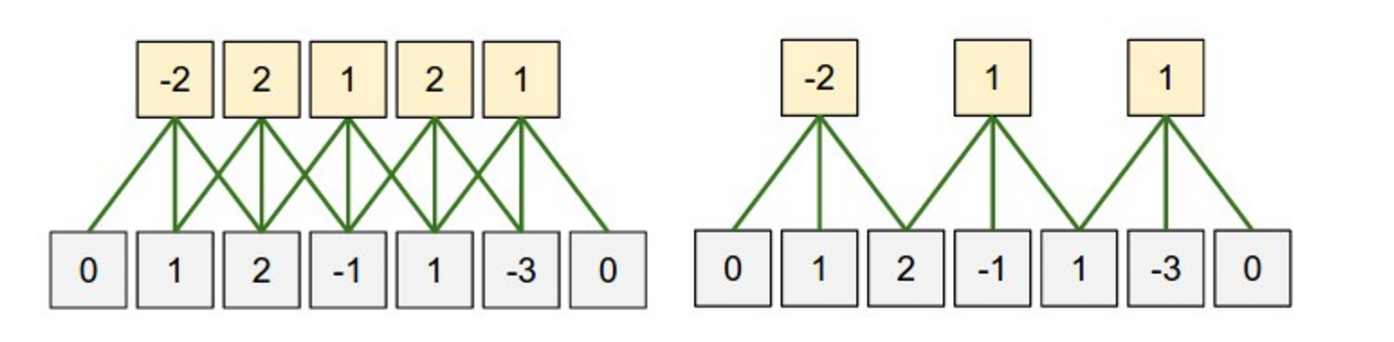
\includegraphics[scale=0.4]{./tex/convolution-network/cnn/stride.png}
    \caption{Impact du stride sur la sortie de la convolution}
    \label{stride_fig}
\end{figure}

\begin{figure}
    \centering
    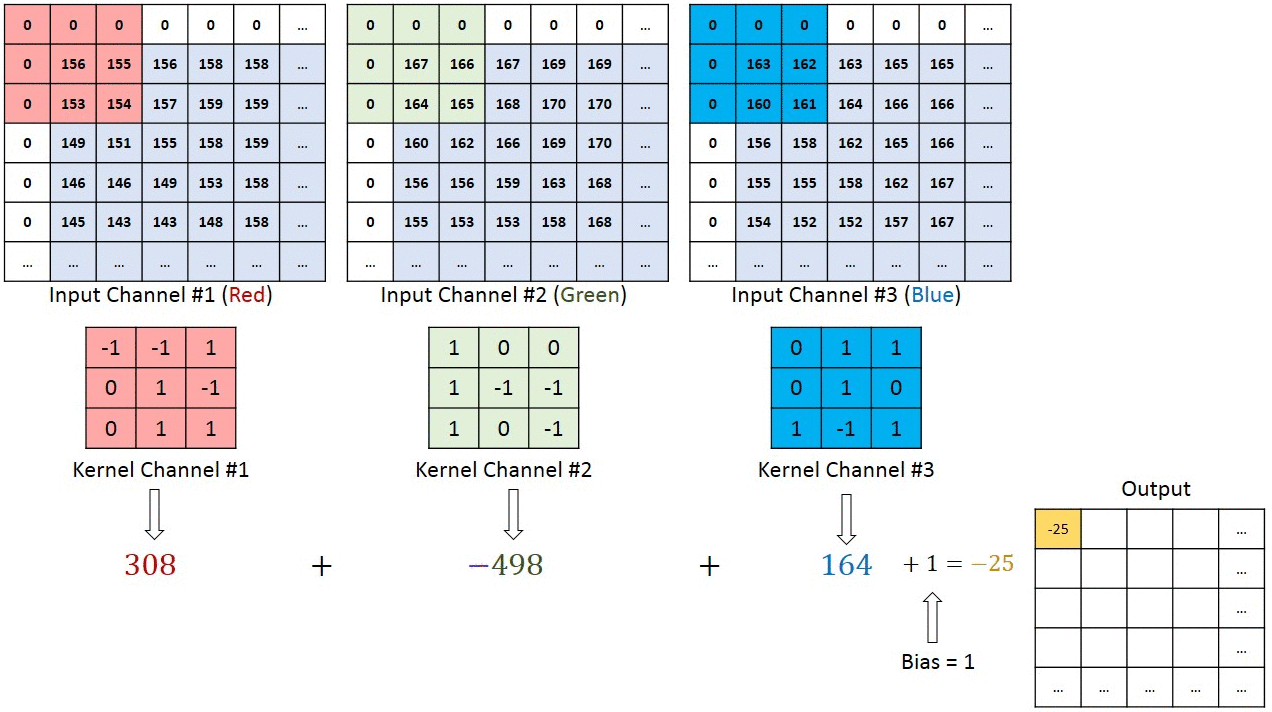
\includegraphics[scale=0.3]{./tex/convolution-network/cnn/conv_filtre.png}
    \caption{Exemple d'une convolution par filtre}
    \label{conv_fil}
\end{figure}

\begin{figure}
    \centering
    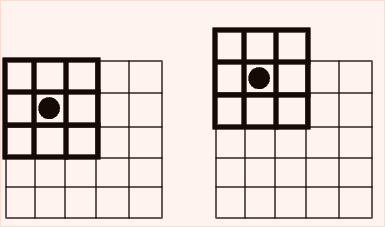
\includegraphics[scale=0.4]{./tex/convolution-network/cnn/padding.png}
    \caption{Problématique de la dimension du filtre: gauche (valide), droite (invalide)}
    \label{centre_pb}
\end{figure}

\begin{figure}
    \centering
    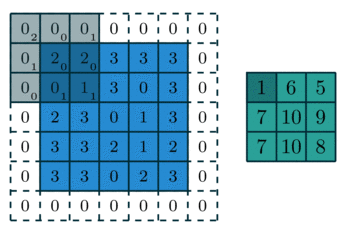
\includegraphics[scale=0.4]{./tex/convolution-network/cnn/padding_.png}
    \caption{Application du 0-Padding}
    \label{padding}
\end{figure}

\subsubsection{Couche de Pooling}
Le \textit{Pooling} est une méthode permettant de compresser (et généraliser) une information locale de la donnée d'entrée. Elle est employée afin de diminuer la dimension des \textit{feature map} tout en conférant une capacité de généralisation à la couche. En effet, le Pooling conserve l'information locale importante, permettant de s'émanciper de détails trop spécifiques (et du bruit).\\

\noindent Le fonctionnement d'une couche de Pooling est comparable à celle d'une couche de convolution si ce n'est qu'elle s'applique sur une \textit{feature map} indépendamment des autres (la profondeur du kernel est de 1). Un filtre (de taille choisie) est appliquée afin de définir \textit{l'environnement local}\footnote{Comparable à une isolation spatiale} et un opérateur est appliqué sur les valeurs d'entrée ciblées par le filtre. La nature de cet opérateur est variable: Max, Average\footnote{Ces deux opérateurs sont les plus fréquents}. Expérimentalement, la fonction Max est la plus utilisée. Sur la Figure \ref{maxpool_fig}, nous pouvons observer l'application d'un Max-Pooling de filtre 2*2.\\

\noindent \textbf{Remarque}: Le Pooling doit être exploitée avec parcimonie. Il est souvent un \textit{bottleneck} pour la vélocité du modèle. De même, son utilisation ne fait pas l'unanimité dans le milieu scientifique. En effet, Geoffrey Hinton, chercheur de renom dans le domaine de l'apprentissage profond, a déclaré: "\textit{The pooling operation used in convolutional neural networks is a big mistake and the fact that it works so well is a disaster."} (Reddit AMA).\\

\noindent Ce scepticisme repose sur plusieurs défauts de cette approche. Le Pooling est une action non évolutive (fixe donc sans apprentissage), ce qui nuit à la capacité de généralisation/spécialisation. De plus, son action est locale à une \textit{feature map}. Il y a donc une perte importante d'informations associées aux relation inter-feature map. Pour finir, le Pooling a une capacité explicative lorsque les couches de convolutions présentent un fort taux d'abstraction. Dans le cas contraire, le filtre est souvent de taille trop faible pour considérer une information discriminante. Augmenter la taille du filtre est envisageable mais le Pooling étant \textit{destructeur}, l'augmentation du filtre aurait des conséquences désastreuses sur la transmission de l'information aux couches supérieures.\\

\noindent Plus récemment, des propositions de fonctions de Pooling ont été faites. Nous pouvons citer:
\begin{itemize}
    \item \textbf{$L_p$ Pooling}\cite{lppool}: Cette approche est issue des études biologiques des cellules vivantes. Elle est définie par: $y_{m,n,k}=\left[\sum_{(i,j) \in R_{mn}} (a_{i,j,k})^p \right]^{\frac{1}{p}}$ avec $R_{mn}$, surface du filtre et k, channel analysé.\\

    Il s'agit de la norme $L_p$ des valeurs ciblées par le filtre du Pooling. Ainsi, si p=1 alors $L_p$ correspond à l'average Pooling. Si $p= \infty$, $L_p$ correspond au max Pooling. Cette méthode permet de réaliser un compromis entre l'isolation discriminante d'une information et la généralisation du message locale.

    \item \textbf{Mixed Pooling}\cite{mixedpool}: Cette méthode combine max Pooling et average Pooling au sein d'une combinaison linéaire dont les coefficients pondérateurs dépendent d'un paramètre $\lambda$ tel que $\lambda \in \mathcal{U}(0,1)$. Ainsi, nous obtenons: $$y_{m,n,k}=\lambda \  max_{R_{mn}}a_{i,j,k}+(1-\lambda)\frac{1}{|R_{mn}|}\sum_{(i,j)\in R_{mn}}a_{i,j,k}$$

    Expérimentalement, elle présenterait de meilleurs résultats que l'approche max ou average tout en proposant une plus grande résistance au sur-apprentissage.

    \item \textbf{Gated max-average Pooling}\cite{mixedpool}: Cette approche est similaire à \textit{Mixed Pooling} mais considère l'état de la surface couverte par le Pooling. En effet, \textit{Mixed Pooling} applique un coefficient indépendamment des valeurs couvertes par le filtre de Pooling. \textit{Gated max-average Pooling}, au contraire, va réaliser une pondération évolutive selon les valeurs couvertes par le filtre. On suppose x, valeurs couvertes par le filtre de Pooling et w, "Gate" du Pooling. Cette idée est traduite par:

    $$ f_{gate}=\sigma(w^Tx)f_{max}(x)+(1-\sigma(w^Tx))f_{avg}(x)$$
    $$\sigma(w^Tx)=\frac{1}{(1+exp(-w^Tx))} $$

    La "Gate" peut être unique à un réseau, une couche, à une région de la couche mais identique sur toute la profondeur ou au contraire, différente sur toutes les profondeurs. Néanmoins, cela ajoute des paramètres à apprendre et donc un ralentissement de la vitesse d'apprentissage. Cette approche présente des résultats plus performants que \textit{Mixed Pooling}.

    \item \textbf{Stochastic Pooling}\cite{stopool}: Cette méthode choisit une valeur selon une distribution de probabilité définie par $p_i=\frac{a_{i}}{\sum_{k \in R_{mn}}a_k}$ avec $i \in [1, |R_{mn}|]$ et $R_{mn}$, l'ensemble des valeurs isolées par le filtre du Pooling.\\

    Ainsi, plus une valeur est élevée, plus la chance d'être choisie est importante. Cette méthode permet de limiter le sur-apprentissage comparée au max-Pooling en introduisant un comportement probabiliste sur la sélection de la valeur.\\
\end{itemize}
\begin{figure}
\begin{tabular}{cc}
    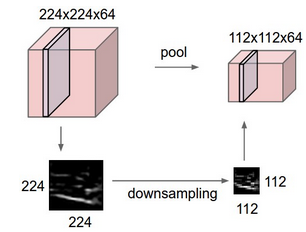
\includegraphics[scale=0.4]{./tex/convolution-network/cnn/pooling_ex.png}  & 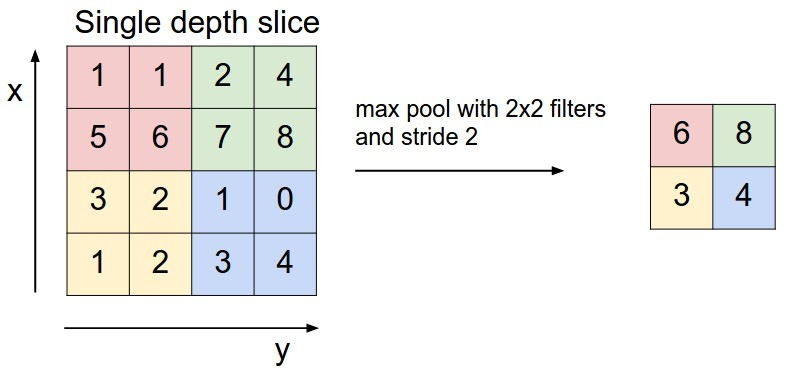
\includegraphics[scale=0.3]{./tex/convolution-network/cnn/maxpool.jpeg} \\
\end{tabular}
\caption{Application du Pooling: Réduction et exemple avec la fonction max selon un filtre 2*2}
\label{maxpool_fig}
\end{figure}

\noindent \textbf{Remarque}: Dans les faits, ces méthodes de Pooling sont assez marginales et peu exploitées. L'écrasante majorité des réseaux actuels exploitant des approches par Pooling reposent sur l'opérateur Max ou Average.\\

\noindent L'opérateur Max est utile lorsque l'on cherche à extraire une information discriminante au détriment des autres. L'objectif est d'isoler les éléments les plus discriminants afin de les analyser par la suite (notamment par un réseau Full-Connected). Cette approche est très utile pour la classification d'images par exemple. En effet, pour classer, un élément discriminant est nécessaire et suffisant. D'autres données moins informatives risqueraient de se comporter comme une forme de bruit.\\

\noindent L'opérateur Average ne se focalise pas sur les élements discriminants du signal mais sur son comportement général. Sa valeur est donc un résumé global de ses caractéristiques et non d'un aspect discriminant spécifique. Cet opérateur est donc moins destructeur mais possède un pouvoir discriminant plus faible.\\

\noindent La couche de Pooling, selon la configuration, peut conserver des informations utiles pour d'autres couches. Par exemple, dans le cas du Max-Pooling, une mémorisation de la localisation de la valeur max sur la matrice de données peut être réalisée. Cette information permet de réaliser des mises à l'échelle (via Unpooling) avec plus de fidélité mais demande de la mémoire pour stocker les valeurs.\\

\noindent \textbf{Remarque}: Expérimentalement, on a tendance à éviter le chevauchement des filtres de Pooling. Ainsi, on exploite un stride en édéquation avec la dimension du kernel pour que chaque valeur de la \textit{feature map} soit analysée une unique fois. Par exemple, dans le cadre d'un kernel 2*2, on aura tendance à utiliser un stride de 2.

\paragraph{Global Pooling}

\noindent Global Pooling est l'équivalent du pooling mais son application n'est pas limitée par la fenêtre correspondant à la taille du filtre. Il ne s'effectue donc pas sur un sous-ensemble (défini par le filtre) d'une \textit{feature map} mais sur l'intégralité d'une \textit{feature map}. Une \textit{feature map} est donc représentée par une unique valeur à l'issu d'un Global Pooling.  Ainsi, supposons une donnée de la forme 15*15*3 avec 3, profondeur\footnote{Nombre de \textit{feature map} présents dans la sortie considérée} de la sortie. La sortie sera donc représentée par un vecteur de dimension dans $R^3$.\\

\noindent Le Global Pooling est une méthode utilisée pour lutter contre le sur-apprentissage et  diminuer le volume des calculs des réseaux convolutifs, notamment de la couche Full-connected réalisant la classification. Les capacités de régulation du Global Pooling s'expriment sous différents aspects:

\begin{itemize}
    \item \textbf{Sans apprentissage}: Étant donné que le Global Pooling considère l'intégralité d'une \textit{feature map}, il n'y a pas d'apprentissage associée à cette couche, ce qui n'ajoute pas de temps d'apprentissage

    \item \textbf{Optimisation de la relation Label - Feature Map}: La couche de Full-connected réalise la prédiction à partir des \textit{feature map}. Les \textit{feature map} sont donc les porteuses d'informations qui doivent retranscrire les spécificités d'un label (catégorie). Il existe un risque important que les feature maps "brutes" soient trop spécifiques du fait des dimensions matricielles élevées de leurs structures, ce qui provoque des dérives vers le sur-apprentissage. L'approche du Global Pooling, en limitant à une valeur par \textit{feature map}, favorise la correspondance entre une \textit{feature map} et une caractéristique générale.

    \item \textbf{Généralisation Spatiale}: En résumant une \textit{feature map} à une valeur, le Global Pooling permet de généraliser l'information. Cette méthode permet donc d'extraire une caractéristique indépendamment de considérations spécifiques due à l'image d'entraînement telles que l'angle de vue, le contraste ou encore la luminosité par exemple.

    \item \textbf{Temps d'apprentissage}: Le Global Pooling limite grandement le nombre de valeurs d'entrée de la couche Full-connected. Cette méthode permet donc d'en diminuer la taille, ce qui rendra le modèle plus rapide à apprendre, à calculer ses prédictions et plus léger d'un point de vue mémoire.
\end{itemize}

\noindent Le Global Pooling est une approche de plus en plus utilisée pour réaliser la liaison entre l'ensemble des couches de convolution et le réseau Full-Connected, remplaçant ainsi la méthode dite \textit{Flatten} classique qui consiste à vectoriser les features map dans leur intégralité. Néanmoins, Global Pooling est très destructeur et présente des faiblesses notamment dans le cas de données textuelles (classification de textes par réseau convolutif par exemple).

\paragraph{k-Max Pooling}
Afin de corriger le comportement destructeur du Global Pooling, k-Max Pooling\cite{kmaxpool} applique l'opérateur pour conserver les k valeurs\footnote{Si k est égal à 1, le comportement est identique à un Global Max Pooling} les plus importantes (au lieu d'une seule pour le Global Pooling). Du fait d'un résultat non unitaire, l'opérateur Average n'est pas exploitable par cette approche.\\

\noindent Le choix de la valeur de k peut être difficile à réaliser. Une valeur trop faible posséderait les mêmes faiblesses qu'un Global Max Pooling et une valeur trop élevée nuirait à la capacité de généralisation recherchée par l'exploitation de ce type de couche. De plus, comme le Pooling s'exerce sur une \textit{feature map} uniquement, la profondeur est à considérer lors du choix de la valeur de k. En effet, en supposant n \textit{feature map} en entrée, la sortie de la couche de k-Max Pooling sera de dimension $n*k$.\\

\noindent Les couches de convolution permettent d'extraire l'information utile d'un signal. Néanmoins, elles sont directement dépendantes de la qualité de la donnée en entrée. Une donnée trop bruitée provoquera un résultat médiocre peu importe la qualité du modèle employé. Une couche de Pooling mal exploitée peut être une source de contre-performance du réseau du fait de son grand pouvoir destructeur. Il est donc intuitif de penser que dans un réseau qui cumule plusieurs couches de Pooling, le pouvoir généralisant doit être progressivement exploité pour ne pas perdre d'informations en amont des couches convolutives. En d'autres mots, dans le cadre du k-Max Pooling, k doit avoir une valeur plus importante au niveau des couches basses et une valeur plus faible au niveau des couches élevées.\\

\noindent Pour répondre à cette problématique, Dynamic K-Max Pooling \cite{kmaxpool} a été proposé. Cette approche propose une détermination automatique de la valeur de k en fonction de l'architecture du réseau et de la position de la couche de Pooling dans ce dernier.\\

\noindent La valeur de k est définie par: $k_l=max(k_{top},\lceil\frac{L-l}{L}*s\rceil)$ avec $k_{top}$, valeur minimale de k pour les couches supérieures, L, nombre total de couches de convolution dans le réseau, l, position de la couche où le Pooling est appliqué et s, dimension\footnote{A l'origine, cette approche de Pooling a été proposée pour l'analyse de texte. De ce fait, s correspond à la dimension du texte en entrée. Il est possible de généraliser à un signal 2D comme un image mais il est probable que la fonction doive être modifiée pour mieux correspondre aux caractéristiques d'une image} de la \textit{feature map}.\\

\noindent La fonction proposée permet d'avoir une diminution progressive de la valeur de k (jusqu'au seuil critique $k_{top}$ et ainsi, d'augmenter le pouvoir discriminant des couches de Pooling en adéquation avec les caractéristiques informatives des données entrantes. La fonction proposée par \cite{kmaxpool} est "arbitraire" et ne repose sur aucune véritable justification mathématique si ce n'est l'intuition des auteurs. Elle peut être modifiée afin d'obtenir un comportement plus spécifique sur la vitesse de décroissance. De plus, elle est spécifique à une donnée textuelle. Dans le cadre d'une image, il est pertinent d'envisager une autre fonction qui sera en adéquation avec le comportement d'un signal 2D.

\subsubsection{Couche de Unpooling}
Le Unpooling est une approche de \textit{Upsampling}, i.e l'augmentation de la dimension de représentation d'une données. Cette approche est utilisée après une une couche de pooling lorsqu'une mise à l'échelle est nécessaire. Elle exploite la capacité de la couche de pooling à conserver des informations de position\footnote{Dans le cas de l'average-pooling, ce n'est pas nécessaire} (notamment pour Max-Pooling). La configuration de la \textit{feature map} de sortie dépend de la méthode de pooling choisie. Ainsi, dans le cas d'un max-pooling, seule la valeur à la position correspondant à la position de la valeur max sur la donnée d'entrée (bornée par la surface couverte par le filtre) sera définie, les autres valeurs étant considérées comme 0. Une illustration est visible sur la Figure \ref{unpooling}. \\

\begin{figure}
    \centering
    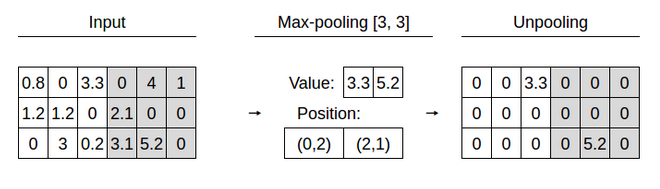
\includegraphics[scale=0.4]{./tex/convolution-network/cnn/unpooling2.png}
    \caption{Exemple de Max-Unpooling statique}
    \label{unpooling}
\end{figure}

\noindent L'exemple présenté est statique (réutilise les valeurs max sans apprentissage). Une approche similaire consiste à ne pas utiliser la valeur max de la \textit{feature map} d'entrée et à appliquer un autre filtre, entraînable, afin de définir les valeurs de la nouvelle \textit{feature map}. De ce fait, seules les informations de position sont utilisées. Un exemple est visible sur la Figure \ref{unpooling2}.

\begin{figure}
    \centering
    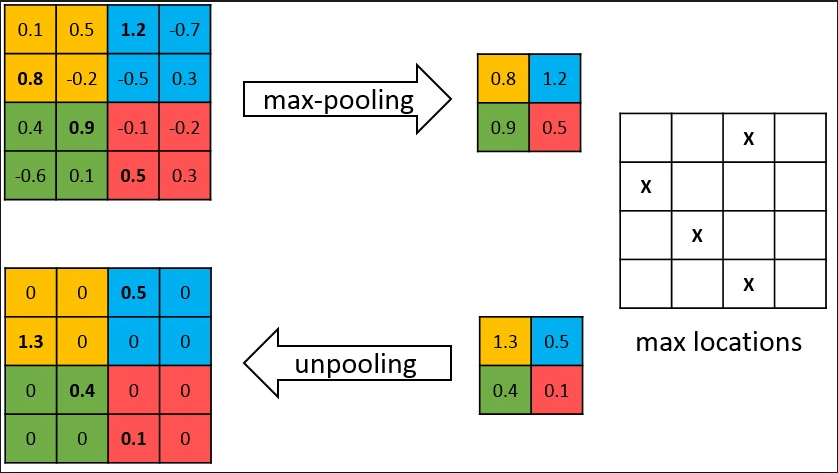
\includegraphics[scale=0.3]{./tex/convolution-network/cnn/unpooling.png}
    \caption{Exemple de Max-Unpooling dynamique}
    \label{unpooling2}
\end{figure}

\subsubsection{Couche de convolution 1*1}
Un cas particulier est la couche de convolution 1*1. Au premier regard, cette convolution semble non pertinente voire sans intérêt\footnote{Pour les lecteurs sensibilisés au traitement du signal, c'est un quasi non-sens}. Néanmoins, du fait de la considération obligatoire de la profondeur de la donnée d'entrée, ce type de convolution possède un intérêt certain. En effet, elle a la capacité de modifier la profondeur de sortie de la couche de convolution où la profondeur correspondra au nombre de filtre présent dans la couche de convolution 1*1. Supposons une donnée d'entrée de dimension X*Y*Z avec Z, profondeur de cette donnée. L'application d'une couche de convolution 1*1 avec N filtres créera une sortie de dimension X*Y*N. Cette méthode complète l'approche par pooling. En effet, le pooling limite la dimension de la \textit{feature map} et la convolution 1*1 limite la profondeur de sortie, i.e le nombre de \textit{feature map}. \\

\noindent Cette convolution ne se focalise que sur la valeur ciblée par le filtre sans considération des corrélations locales mais tient compte de l'ensemble des channels de la donnée d'entrée\footnote{La profondeur est toujours considérée dans son intégralité}. Elle permet donc d'ajouter de la non-linéarité dans l'architecture du réseau\footnote{Ce qui est souvent favorable aux performances du réseau}.

\subsubsection{Couche de convolution dilatée}
Les couches de convolution dilatées\cite{dilate} introduisent un nouveau paramètre: \textbf{le taux de dilatation}. Le taux de dilatation détermine l'espace entre chaque valeur effective du kernel. Par exemple, un kernel 3*3 avec un taux de dilatation de 2 deviendra un kernel de 5*5 car le filtre ne se focalisera pas sur des éléments adjacents $a_i$, $a_{i+1}$ mais sur des éléments distants en accord avec le taux de dilatation. Ainsi, pour une dilatation de 2, les éléments ciblés seront $a_i$, $a_{i+2}$. Les valeurs contenues dans le champ réceptif mais non effectives auront une valeur imposée à 0 (car le poids associé sera nul). La Figure \ref{dilate} illustre ce type de convolution.\\

\noindent Cette approche permet d'élargir le champ d'analyse de la couche en conservant le même coût de calcul. Elle est très utilisée pour la détection d'entités ou la segmentation car elle offre un bon compromis de performance. Elle permet une analyse générale d'une image sans multiplier les convolutions ou l'utilisation de filtres larges qui sont très gourmands en ressources. Par exemple, supposons un filtre 3*3 (stride 1) classique. En combinant 3 couches composées de ce filtre, le champ réceptif de la dernière couche sera de 7*7 ($3*3 \rightarrow 5*5 \rightarrow 7*7$). Au contraire, avec une dilatation de 2, la surface couverte sera de $15*15$.

\begin{figure}
    \centering
    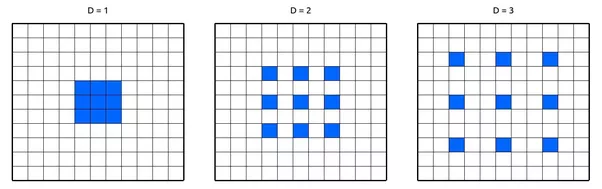
\includegraphics[scale=0.4]{./tex/convolution-network/cnn/dilated.png}
    \caption{Exemple d'une convolution dilatée}
    \label{dilate}
\end{figure}

\subsubsection{Couche de convolution transposée}
\textbf{Remarque}: Cette couche est aussi appelée \textit{fractionally strided convolutions} ou \textit{déconvolution}. L'appellation "déconvolution" est un abus de langage. Cette couche ne réalise pas une déconvolution au sens mathématique du terme.\\

\noindent Une couche de convolution transposée a pour objectif de mettre à une dimension \textbf{supérieure} choisie, une donnée d'entrée. Il s'agit ainsi d'une technique de \textit{Upsampling}. C'est très utilisé en segmentation afin de mettre à l'échelle la sortie d'un réseau convolutif.\\

\noindent Son fonctionnement est comparable à une convolution standard avec l'application de padding (ajout de 0 arbitraire) afin de compléter la donnée d'entrée et mettre à l'échelle voulue la \textit{feature map} de sortie. Le padding dépend de la taille du filtre choisie, du stride et de la dimension de sortie du \textit{feature map}. Deux exemples sont visibles sur la Figure \ref{local_fig}.\\

\noindent Les couches de convolution transposées permettent uniquement de conserver les dimensions des features map. Ainsi, supposons une entrée N alors l'application d'une couche de convolution sur cette entrée puis d'une couche de déconvolution (avec le même paramétrage de couche que la couche de convolution) permettra d'obtenir une sortie de même dimension que N. Par contre, la sortie n'est \textbf{pas égale} à N ! D'où l'abus de la dénomination \textit{déconvolution} qui est faux mathématiquement parlant.

\begin{figure}
\centering
\begin{tabular}{cc}
    \includegraphics[scale=0.4]{./tex/convolution-network/cnn/transposed.png}  & \includegraphics[scale=0.4]{./tex/convolution-network/cnn/transpose2.png} \\
\end{tabular}
\caption{Exemple de convolution transposée: Gauche: entrée 2*2 sans stride, Droite: Entrée 3*3 avec stride de 1}
\label{local_fig}
\end{figure}

\subsubsection{Couche de Depthwise/Pointwise}
\label{depthwiseconv}
Bien qu'efficaces, les couche de convolution standards restent gourmandes en temps de calcul et en mémoire nécessaire pour stocker le modèle. Dans des contextes particuliers avec des limitations de ressources tels que l'embarqué ou encore les smartphones/tablettes, l'utilisation de modèle très profond classique n'est pas envisageable pour cause de limitation matérielle. En plus des méthodes standards de réduction vues dans les Sections précédentes, il est possible d'agir au niveau de l'architecture-même des couches de convolutions avec les couches de \textbf{Depthwise/Pointwise} (ou separable depthwise). Ce type de couche a été popularisé par la création de l'architecture \textit{MobileNet}\cite{mobilenet} crée par Google afin de répondre aux problématiques des prédictions sur smartphone. \\

\noindent Le comportement général de ce type de couche est comparable aux couches de convolution standards. La différence se situe au niveau des spécificités du nombre de filtres et de leurs dimensions. Une couche de depthwise/pointwise se découpe en deux parties: la partie depthwise et la partie pointwise. La couche depthwise est comparable à une couche de convolution standard mais avec \textbf{uniquement} un filtre. Dans une couche de convolution depthwise/pointwise, il n'y a qu'une couche depthwise. La couche pointwise est comparable à une couche de convolution standard avec un filtre de dimension \textbf{1*1} et s'applique sur la sortie \textit{intermédiaire}\footnote{Avant l'étape d'addition par rapport à une convolution standard} de la couche depthwise. Cette couche peut être cumulée N fois. Une illustration de cette couche est visible sur la Figure \ref{depthwise_fig}.\\

\begin{figure}
    \centering
    \includegraphics[scale=0.3]{./tex/convolution-network/cnn/depthwise.png}
    \caption{Exemple d'une couche Depthwise/Pointwise avec 2 filtres}
    \label{depthwise_fig}
\end{figure}

\noindent Étudions dorénavant les bénéfices de ce type d'approche. Supposons une entrée (matrice carrée) de dimension X*X*M avec M, profondeur de l'entrée. On lui applique N filtres (composés de sous-filtres en accord avec la profondeur de la donnée d'entrée). On supposera que chaque filtre possède une dimension identique de taille K*K. Le coût de calcul d'une couche de convolution standard est donc de (X*X)*M*(K*K)*N\footnote{On suppose un stride de 1 et un 0-padding nécessaire pour conserver la même dimension entre les données d'entrée et la \textit{feature map} de sortie}.\\

\noindent Considérons maintenant une couche depthwise/poitnwise. On a alors:

$$D_{depthwise/poitnwise}=D_{depthwise}+D_{pointwise}$$
$$D_{depthwise}=(X*X)*M*(K*K)*1$$
$$D_{pointwise}=(X*X)*M*(1*1)*N$$
$$D_{depthwise/poitnwise}=(X*X)*M*(K*K)*1+(X*X)*M*(1*1)*N$$
~~\\
La différence de coût de calcul est donc définie par: $$\frac{(X*X)*M*(K*K)*1+(X*X)*M*(1*1)*N}{X*X)*M*(K*K)*N}=\frac{1}{N}+\frac{1}{K^2}$$
~~\\
Ce résultat permet d'évaluer la pertinence de ce type de couche. En effet, on peut observer que plus le nombre de couche est importante (N) et/ou la taille du filtre grand (K), plus l'économie en temps de calcul est important. Cette économie est associée au temps de calcul machine et au temps d'apprentissage, le rapport étant identique pour les deux économies. Ainsi, pour les réseaux très profonds sur des supports de faible puissance, cette approche propose une solution performante.\\

\noindent Néanmoins, cette approche donne des résultats moins performants bien que ce défaut soit négligeable face au temps machine et d'apprentissage. L'utilisation ou non de ce type de couche relève des spécificités du problème à résoudre. Il est intéressant de noter que cette approche a été très sollicitée (et avec succès) sur les supports mobiles comme les smartphones.

\subsection{Conversion d'une couche Full-Connected en couche de convolution}
\label{convfctoconv}
Une couche Full-Connected, par un "jeu de couches", peut être remplacée par une approche exclusivement convolutive. Bien que cette approche puisse sembler \textit{tricky}, elle est très utile afin d'optimiser certains réseaux qui exigent un calcul de prédiction rapide en limitant la redondance de calcul (algorithmes de \textit{Tracking} par exemple).\\

\noindent Observons la Figure \ref{fulltoconv}. En haut, un réseau convolutif classique avec deux couches Full-Connected en fin de réseau finalisées par un \textit{Softmax}. Une sortie \textit{Softmax} est caractérisée par une couche composée de neurones comportant autant de sortie que de classes discriminées suivie d'une activation par une fonction \textit{Softmax}. Dans notre exemple, supposons que le réseau discrimines 4 classes, i.e 4 neurones sur la couche de sortie.\\

\noindent La première couche de Full-Connected est connectée à une sortie de dimension 5*5*16. Un neurone possède donc 5*5*16 entrées distinctes. Observons le réseau entièrement convolutif (réseau du bas sur la Figure \ref{fulltoconv}). La couche Full-Connected est remplacée par une couche convolutive de kernel 5*5 et de profondeur 400. La sortie de cette couche sera donc de dimension 1*1*400. Cette couche de convolution est donc déterminée par 400 neurones où seul un neurone caractérise un filtre. Un kernel, par convention, s'applique sur toute la profondeur. Ainsi, chaque neurone de la couche de convolution reçoit 5*5*16 (hauteur*largeur*profondeur) valeurs pondérées par des poids distincts (et apprenants). Par conséquent, ces deux architectures sont mathématiquement identiques car le logit formé est issu d'une relation linéaire similaire et la couche présente autant de neurones.\\

\noindent Afin de réaliser la conversion, il faut donc créer une couche de convolution dont la dimension du kernel est égale à la dimension (hauteur et largeur) des features map en entrée. Le nombre de filtre de cette couche de convolution est égale au nombre de neurones de la couche Full-Connected.

\begin{figure}
    \centering
    \includegraphics[scale=0.4]{./tex/convolution-network/cnn/fctoconv1.png}
    \caption{Exemple d'une conversion de couche Full-Connected vers une structure convolutive}
    \label{fulltoconv}
\end{figure}

\subsection{Convolutional Neural Network (CNN) et Fully Convolutional Network (FCN)}
Avec l'évolution de la Recherche, une famille d'architecture a été crée: \textit{Fully Convolutional Network}\cite{fcn} (FCN).\\

\noindent Contrairement à l'architecture CNN standard, FCN n'utilise pas de couche Full-Connected mais exclusivement des couches convolutives\footnote{D'où le nom Fully Convolutional Network}. La prise de décision du réseau est donc assurée par des couches convolutives tout comme l'extraction d'attributs.\\

\noindent Un réseau FCN va donc essayer d'extraire les informations et de prendre une décision selon des données \textbf{spatialement indépendante} du fait de l'isolation réalisée par le fonctionnement de la convolution. Chaque \textit{sous-décision} de la couche convolutive est basée sur l'information isolée par la taille du filtre. Au contraire, CNN aura tendance à considérer l'information dans sa \textbf{globalité} du fait de l'utilisation de couches Full-Connected qui exploite intégralement les données. Il n'y a donc pas de considération de \textit{localité}. Ces dernières années, les réseaux FCN gagnent en popularité du fait de leur efficacité similaire et de leur plus grande vitesse d'apprentissage. De même, un FCN permet une plus grande robustesse face à des données de dimensions variables\footnote{Les couches Full-Connected sont dépendantes de la dimension de la donnée d'entrée} tout en réalisant la conversion d'échelle plus rapidement.

\subsection{Les modèles convolutifs de référence}

\subsubsection{AlexNet}
AlexNet\cite{alexnet}(2012) est une référence historique du Deep Learning. Il est le modèle précurseur des architectures convolutives (reposant sur l'architecture LeNet développée par Lecun) et a présenté des résultats remarquables en gagnant le 2012 ILSVRC\footnote{Il s'agit d'une des compétions - voire la compétition - la plus prestigieuse et compétitive de vision par ordinateur} (ImageNet Large-Scale Visual Recognition Challenge) avec 10\% d'erreur en moins que le 2nd. Il constitue un cas d'école pertinent pour apprendre les fondations d'un réseau convolutif (couche de convolution, max-pooling, dropout, ReLu...) et a été défini pour classer 1000 catégories au plus. Du fait de son ancienneté, il tend à devenir "obsolète" aujourd'hui.

\subsubsection{ZF Net}
ZF Net\cite{zfnet}(2013) est un modèle basé sur AlexNet et vainqueur du 2013 ILSVRC. La différence majeure se situe sur la taille des filtres, notamment des premières couches. L'idée derrière cette réduction était de limiter un maximum la perte d'information associée à un filtre trop grand (trop généraliste) de la donnée initiale. De plus, il n'a été entraîné que sur 1.3 million d'image et non 15 milions comme AlexNet.\\

\noindent L'apport majeur de ce modèle (et du papier de recherche associé) est la méthode de visualisation DeConvNet (Deconvolutional Network). Cette méthode permet d'examiner les caractéristiques d'activation des différentes couches et d'offrir un aperçu de ce que "voit" et discrimine la couche observée. Cette architecture a permis de mieux comprendre le comportement interne des réseaux convolutifs et leurs critères de discrimination\footnote{On est encore loin de comprendre parfaitement le fonctionnement des réseaux neuronaux. C'est toujours un sujet de recherche très intense et d'une nécessité prioritaire}. On le nomme DeConvNet du fait de l'inversion de la transformation réalisée. Au lieu de passer de "pixels à map feature", ce réseau passe de "map feature à pixels".

\subsubsection{VGG Net}
VGG Net\cite{vggnet}(2014) est un finaliste (mais perdant) de 2014 ILSVRC. Ce réseau exploite une architecture "simple" mais profonde. En effet, ce modèle se limite à cumuler des couches de convolution utilisant des filtres 3*3 - stride 1 et des couches de max-pooling 2*2 - stride 2. La contribution principale de ce modèle a été de montrer que la profondeur est un composant critique de bonne performance. Néanmoins, c'est un modèle lourd (en ressources matérielles et paramètres) bien qu'il puisse être grandement simplifié en supprimant des couches de Full-connected sans une perte significative de performance. Il s'agit d'un modèle encore très utilisé aujourd'hui.

\subsubsection{GoogleNet/Inception}
GoogleNet\cite{googlenet}(2014) est le vainqueur du 2014 ILSVRC. L'architecture de ce modèle est très novatrice (elle s'inspire, néanmoins, de l'approche Network in Network\cite{nin})\footnote{Nous n'aborderons pas ce papier. Il a une importance théorique mais n'apporte pas d'élément applicatif concret dans le cadre de ce cours}. Elle s'oppose au dogme du modèle séquentiel (succession de couches à flux unitaire) et propose une approche en "largeur" (en parallèle). Ce modèle a ainsi proposé une nouvelle forme de \textit{block}: \textbf{l'Inception module}. Sa structure est représentée sur la Figure \ref{inception}.\\

\begin{figure}
    \centering
    \includegraphics[scale=0.3]{./tex/convolution-network/classifier/inception.png}
    \caption{Architecture de l'Inception module}
    \label{inception}
\end{figure}

\noindent L'Inception module se démarque par la mise en parallèle de différentes couches de convolution appliquées sur une même source d'entrée dont les \textit{feature map} produites sont \textbf{concaténées} à la fin du bloc. Cette mise en parallèle des couches permet de créer différents \textit{flux} indépendants et différenciés les uns des autres. Chaque block peut avoir sa propre topologie, ce qui rend le modèle difficile à implémenter du fait de cette liberté. Évaluer la topologie d'un block est délicat et relève essentiellement de l'intuition. Il est important de relever la présence de convolution 1*1. Une approche naïve serait de les supprimer, leurs importances semblant être secondaires. Néanmoins, ce serait une erreur majeure. En effet, ces convolutions possèdent deux caractéristiques critiques dans le cadre de ce module:

\begin{itemize}
    \item \textbf{Réduction de dimension}: Les convolutions 1*1 possèdent la capacités de réguler la profondeur de la sortie d'une couche. Cette capacité est primordiale dans le cas de l'Inception module afin d'éviter une explosion inévitable de la dimension de sortie. Elle permettent ainsi de maîtriser la profondeur souhaitée d'une des branches du modules en sortie pour la concaténation (branche 3*3 max pooling) ou de diminuer la profondeur de la donnée d'entrée sur les branches 3*3 convolutions et 5*5 convolutions. En effet, l'application de filtre volumineux est gourmand en temps machine. Réduire la dimension de la donnée à observer favorise la vélocité du modèle. Les convolutions 1*1 permettent ainsi de réguler la dimension des données internes au module en maîtrisant les dimensions de sortie et en optimisant les dimensions de la données d'entrée pour favoriser un bon rapport performance/temps.

    \item \textbf{Non-linéarité}: Les convolutions 1*1 sont suivies d'une activation ReLu. De ce fait, elles permettent la mise en place de non-linéarité dans le module. Les couches de convolution étant linéaires dans leurs formes fondamentales, cet ajout ne peut être que bénéfique.
\end{itemize}

\noindent Cette architecture a eu plusieurs améliorations. La plus moderne est l'Inception-v4\cite{inceptionv4} qui propose une approche liant l'architecture Inception et Resnet.

\subsubsection{Xception}
Le modèle Xception\cite{xception}(2016) a été inventé par François Chollet, chercheur de Google à l'origine du framework \textit{Keras}. Xception propose une approche \textit{extrême} de l'approche \textit{Inception} d'où son appellation.\\

\noindent Afin de comprendre l'idée proposée par François Chollet, revenons sur le modèle Inception standard. Sur la Figure \ref{xception}, nous pouvons observer deux block Inception. A gauche, un block arbitraire (topologie variable) et à droite, un block simplifié avec une structure uniforme. Supposons un block de N flux. Par un jeu de manipulation, nous pouvons remplacer les N couches de convolution 1*1 indépendantes en une couche 1*1 unique de dimension N*P avec P profondeur des sorties des couches 1*1 indépendantes\footnote{On supposera les sorties uniformes}. Les \textit{feature map} de la couche 1*1 unitaire seront alors divisés en N parties sans chevauchement et alimenteront les différents flux de manière indépendante. Cette approche peut être poussée à \textit{l'extrême} en associant un flux à une unique \textit{feature map}. Une représentation graphique est visible sur la Figure \ref{xception2}. Le postulat du modèle Xception est une hypothèse plus forte que l'hypothèse d'Inception: il suppose que les corrélations inter-channels (profondeur) et les corrélations spatiales (largeur et longueur d'une \textit{feature map}) peuvent être complètement traitées séparément et non par sous-groupes.\\

\noindent Cette approche isolante est très similaire à une convolution Depthwise/Pointwise. Une différence majeure existe: une couche de Depthwise/Pointwise réalise une convolution standard pour créer les \textit{feature map} intermédiaires qui seront alors traitées par des convolutions 1*1. \textit{Extreme Inception} réalise exactement l'inverse. Les créateurs du modèle ne justifie pas concrètement le réel impact de cette inversion si ce n'est par leur intuition. De plus, dans un block Inception, une activation ReLu est appliquée entre les différentes couches afin d'appliquer de la non-linéarité, ce n'est pas le cas avec les couches Depthwie/Pointwise. Cette spécificité permet de mettre en avant un résultat remarquable. Alors que la non-linéarité est bénéfique dans le cas du block Inception standard\cite{inceptrelu}, elle semble être néfaste pour les blocks Extrem Inception avec Deptwise/Pointwise\cite{xception}. Ce résultat a été vérifié expérimentalement. Il est difficile de justifier clairement ce résultat mais l'idée principale repose sur la différence de profondeur. En effet, dans le block Inception standard, la profondeur de la données d'entrée dans un flux est profonde alors que dans un block Extrem Inception, la \textit{feature map} est unitaire. L'hypothèse est donc qu'appliquer une régularisation sur une donnée peu profonde provoque une perte d'informations trop importante.\\

\noindent La spécificité de la couche Depthwise/Pointwise permet ainsi de créer un réseau très simple d'implémentation. En effet, un block Extreme Inception n'est donc rien d'autre qu'une couche de Depthwise/Pointwise. L'architecture générale est standard et ne présente pas de particularité notable si ce n'est l'utilisation des \textit{résidus} (voir Section \ref{resnet} pour plus de détails sur cette notion).

\begin{figure}
    \centering
    \includegraphics[scale=0.4]{./tex/convolution-network/classifier/xception.png}
    \caption{Architecture de l'architecture Xception: à gauche, un block standard et à droite un block simplifié (topologie uniforme)}
    \label{xception}
\end{figure}

\begin{figure}
    \centering
    \includegraphics[scale=0.4]{./tex/convolution-network/classifier/xceptionv2.png}
    \caption{Architecture de l'architecture Xception: à gauche, un block Inception reformulé et à droite un block Inception dans sa forme extrême}
    \label{xception2}
\end{figure}

\subsubsection{Microsoft Resnet}
\label{resnet}

Resnet\cite{resnet}(2015) est le vainqueur de 2015 ILSVRC. Son taux d'erreur est exceptionnel (3,6\%). Un homme, en fonction de son expertise, obtient un taux d'erreur d'environ 5 à 10\%. Cette architecture est donc la première à faire significativement mieux que l'homme dans le cadre de cette compétition. Cette architecture repose sur le \textbf{Residual Block}. Une illustration est visible sur la figure \ref{residual}.\\

\begin{figure}
    \centering
    \includegraphics[scale=0.3]{./tex/convolution-network/classifier/residual.png}
    \caption{Architecture du Residual Block}
    \label{residual}
\end{figure}

\noindent Un \textit{Residual Block} est caractérisé par la non-perte de la donnée d'entrée. Ainsi, la sortie de ce block calcule un changement de faible ampleur (un "Delta") afin d'obtenir une version légèrement altérée de la donnée d'entrée. Pour conserver la donnée d'entrée, une concaténation est réalisée à la sortie du block où la sortie des couches internes est \textbf{additionnée}\footnote{Au sens strict du terme, non concatenée} à la donnée d'entrée\footnote{En cas de dimension différente entre l'entrée et la sortie des couches internes du bloc, du 0-padding et/ou des convolutions 1*1 sont utilisées}. Cette architecture favorise un bon apprentissage en facilitant la propagation d'un gradient "valide", notamment en luttant contre le problème de \textit{vanishing gradient}. L'idée derrière la notion de \textit{Résidus} est qu'il est plus facile d'approximer une fonction qui nullifie les résidus plutôt que d'approximer une fonction identité (Figure \ref{residual2}) . Néanmoins, son efficacité théorique n'est pas démontrée malgré une efficacité empirique et expérimentale incontestable.\\

\begin{figure}
    \centering
    \includegraphics[scale=0.3]{./tex/convolution-network/classifier/resnet2.png}
    \caption{Intuition sur la notion de Résidus}
    \label{residual2}
\end{figure}

\noindent \textbf{Important}: Les architectures \textit{state-of-the-art} reposent essentiellement sur ce type d'architecture\footnote{Plusieurs architectures peuvent être cumulées !}. Il est souvent pertinent de considérer ce type de réseau convolutif lorsqu'un choix par défaut s'impose.

\subsubsection{ResNet et améliorations}
Du fait de l'efficacité des réseaux Resnet, la recherche est active autour de cette architecture. Plusieurs améliorations ont été proposées: \\

\paragraph{Wide Residual Network}

\noindent Wide Residual Network\cite{wideres}(2016) propose une architecture qui s'étend en "largeur"\footnote{Ne pas confondre ! Il y a une augmentation sur un unique flux de couches (ajout de filtres ou d'un DropOut par exemple) uniquement. L'augmentation se fait en largeur car elle ajoute des entités sur une couche ciblée au sein d'un même flux, non en largeur avec l'ajout de flux parallèles comme les modèles Inception !} et non uniquement en profondeur comme l'approche initiale des ResNets. La démarche principale consiste augmenter le nombre de filtres par couche ou implanter des couches spécifiques (dropout, 1*1 convolution,...). Ainsi, cette architecture crée plus de \textit{feature map} en interne et possède un plus fort pouvoir de discrimination. Néanmoins, il peut y avoir une hausse du nombre de paramètres donc un temps de calculs et d'apprentissage supérieurs. Pour s'opposer à ce problème, la profondeur est minorée par rapport à la largeur. De plus, les capacités de calculs sont optimisées avec les approches en largeur car le calcul des différentes \textit{feature map} au sein d'une même couche est fortement parallélisable, ce qui favorise la vélocité du modèle. Cette architecture propose aussi l'ajout de DropOut ou de convolutions 1*1 à l'intérieur des blocs. La plus-value de cet article est de montrer qu'un réseau ResNet ne doit pas être que profond mais favoriser son expansion en largeur aussi. Une illustration de cette architecture est représentée sur la Figure \ref{wide}.

\begin{figure}
    \centering
    \includegraphics[scale=0.4]{./tex/convolution-network/classifier/wideresnet.png}
    \caption{Architecture d'un Wide Residual block (les étapes de Batch normaliszation) et de ReLu ne sont pas affichées) - la largeur des rectangles représentant les couches déterminent graphiquement le nombre de filtres employés pour la couche associée}
    \label{wide}
\end{figure}

\paragraph{Aggregated Residual Transformations for Deep Neural Networks (ResNext)}

\noindent Le réseau ResNext\cite{resnext}(2016) est le modèle arrivé 2nd au 2016 ILSVRC. Cette architecture propose de lier les caractéristiques des modèles ResNet et Inception. La principale caractéristique de ResNext repose sur son expansion en largeur avec l'ajout de flux internes dans un block. Sa différentiation majeure avec l'approche d'Inception est l'utilisation d'une topologie de bloc identique pour chaque bloc. La différenciation des blocks se fait au niveau du facteur de profondeur qui détermine le nombre de flux parallèles au sein d'un block.\\

\noindent L'architecture Resnext propose trois formes de blocks équivalents pour structurer son réseau.

\begin{itemize}
    \item \textbf{Approche ResNet}: Avec cette approche, chaque flux réalise une harmonisation de la dimension indépendamment des autres flux via une convolution 1*1. Les \textit{feature map} issues des différents flux du block sont additionnées. La sortie est alors additionnée avec l'entrée du block.

    \item \textbf{Approche Inception}: Avec cette approche, l'harmonisation de la dimension est mutualisée. Ainsi, l'ensemble des \textit{feature map} issues des flux sont concaténées sans application de convolution 1*1 et produisent une sortie intermédiaire. L'application de la convolution 1*1 est réalisée sur la sortie intermédiaire et les \textit{feature map} obtenues sont additionnées à l'entrée du block.

    \item \textbf{Approche par convolution groupée}: Cette approche repose sur l'implémentation du réseau AlexNet qui a groupé ses couches afin de paralléliser son réseau sur différents GPU. Resnext propose cette méthode en considérant un flux comme un groupe. Ils peuvent donc être partagés sur différents GPU et favoriser la vélocité du modèle. Cette représentation est essentiellement théorique et peu exploitée dans les faits.
\end{itemize}

\noindent Une représentation graphique des différentes architectures du block ResNext est visible sur la Figure \ref{resnext}.

\begin{figure}
    \centering
    \includegraphics[scale=0.4]{./tex/convolution-network/classifier/resnext.png}
    \caption{Différentes représentations de l'architecture d'un block du réseau ResNext: 1) Approche ResNet, 2) Approche Inception, 3) Approche par convolution groupée}
    \label{resnext}
\end{figure}

\paragraph{Densely Connected Convolutionnal Networks (DenseNet)}

\noindent Densely Connected Convolutionnal Networks\cite{densely}(2016) généralise la transmission de l'entrée des blocs ResNet en projetant l'entrée d'une convolution sur l'ensemble des convolutions suivantes et non juste le suivant direct. Ainsi, la $n^{ieme}$ couche possédera une entrée issue de n sources. De même, la $n^{ieme}$ couche transmettra sa sortie aux (N-n) couches suivantes avec N, nombre total de couche. Il y a donc $\frac{N(N+1)}{2}$\footnote{Équivalent à la somme de 1 à n} connexions dans l'ensemble du réseaux issues des divers blocs au lieu de N d'où le nom de \textit{Densely connected}. De plus, l'entrée est \textbf{concaténée} et non additionnée comme dans un bloc ResNet standard. La concaténation implique une augmentation constante de la profondeur de l'entrée transférée à chaque bloc. L'ajout de convolution 1*1 et de pooling est donc une nécessité pour éviter l'explosion du nombre de données en entrée. Veuillez vous référer à l'article \cite{densely} pour plus de détails sur cette régulation. \\

\noindent Le réseau DenseNet, visible sur la Figure \ref{DenseNet}, est composé de plusieurs Dense block séparés par un block de transition formé d'une convolution 1*1 et d'un Pooling afin de redimensionner les \textit{feature map}. Ce redimensionnement pose problème car les \textit{feature map} des block précédents ne sont plus de même dimension que les block qui suivent. De ce fait, la propagation se limite à un Dense block et non à l'ensemble du réseau.

\noindent La conversion de l'addition vers la concaténation apporte une plus-value importante. La concaténation préserve la structure de la \textit{feature map} peu importe l'éloignement du bloc par rapport au bloc considéré. Cette différence permet de s'opposer au problème de corruption de l'information transférée ou de son effacement qui augmente alors que le nombre de \textit{feature map} additionnées augmente linéairement. De plus, le modèle peut apprendre une combinaison optimal entre les features map concatenées, ce qui permet une meilleure interprétation de l'information utile. \\

\noindent Bien que paradoxale, cette approche permet de limiter le nombre de paramètres nécessaire pour créer le modèle. Dans un réseau neuronal, chaque couche lit une entrée donnée par la couche précédente associée et écrit à la couche suivante. La couche actuelle modifie donc l'état mais transmet aussi l'information importante à conserver. Cette information est conservée, dans les réseaux ResNet, par addition avec l'identité de l'entrée. Cependant, il a été montré que certaines couches contribuent peu voire produisent de l'information redondante (il se peut qu'elles redéfinissent une information perdues déjà calculée précédemment dans le modèle) et donc, peuvent être supprimées. Afin de considérer cette particularité, la structure Densely connected propose une meilleure mémoire de la donnée utile et des modifications réalisées en projetant l'information sur l'ensemble des blocs et non uniquement le suivant. Cette propagation (et conservation) de l'information permet de limiter grandement le nombre de couches/blocs et ainsi de limiter le nombre de paramètres, rendant le modèle plus léger et rapide à apprendre. L'intuition derrière cette idée peut être contre-intuitive. Pour une explication détaillée, veuillez vous référer à l'article associé \cite{densely}. La structure d'un réseau Densely Connected est visible sur la Figure \ref{densely}.\\

\begin{figure}
    \centering
    \includegraphics[scale=0.4]{./tex/convolution-network/classifier/dense.png}
    \caption{Architecture d'un réseau Densely Connected}
    \label{densely}
\end{figure}


\begin{figure}
\hspace{-3cm}
    \includegraphics[scale=0.25]{./tex/convolution-network/classifier/densenet.png}
    \caption{Réseau DenseNet}
    \label{DenseNet}
\end{figure}

\paragraph{Stochastic Depth}

\noindent Stochastic Depth\cite{stores}(2016) met en relation le DropOut et les spécificités des \textit{Résidual block} des réseaux résiduels. Afin de limiter l'inter-dépendance des couches du réseaux, les blocks sont conservés (sinon ils sont équivalents à une couche \textit{identité}) selon une probabilité $p_l$. $p_l$ est une probabilité constante (peu optimale) ou linéaire dégressive telle que $p_l=1-\frac{l}{L}*(1-p_L)$ (par défault, $p_L$ est égal à 0.5 et correspond à la valeur limite du dernier block considéré dans le réseau) avec L, nombre total de block et l, le block ciblé. Comme pour le DropOut, durant la phase de test, chaque sortie de residual block (avant union avec la valeur d'entrée du bloc) est active et pondérée selon la valeur du pourcentage d'activation associée. Un exemple illustratif est visible sur la Figure \ref{stores_fig}.

\begin{figure}
    \centering
    \includegraphics[scale=0.4]{./tex/convolution-network/classifier/stores.png}
    \caption{Stochastic Depth routine}
    \label{stores_fig}
\end{figure}

\paragraph{Residual Networks of Residual Networks: Multilevel Residual Networks}

Residual Networks of Residual Networks\cite{RoR}(2016) propose une approche basée sur la structure de groupe. Ainsi, le réseau est composé d'une succession de groupes composés de block à la structure similaire. Le créateur du modèle a utilisé des convolutions 3*3 uniquement de profondeur variable appartenant à $[16,32,64]$. Trois groupes est donc formés en fonction de la largeur des couches. Il n'y a pas d'intersection de groupe, i.e chaque groupe est unique et els groupes sont homogènes. Supposons un réseau avec N block alors un groupe possèdera $\frac{N}{3}$ block. Ce réseau se différencie du ResNet en ajoutant une connexion inter-block pour chaque groupe. Ainsi, les \textit{feature map} en entrée du premier block d'un groupe seront additionnées aux \textit{feature map} de sortie de ce groupe. Un exemple de ce réseau est visible sur la Figure \ref{ror}.\\

\noindent La notion de groupe est variable selon le niveau de coupure P choisi. Ainsi, pour P=1, on considère un groupe uniquement. Le réseau est donc semblable à un ResNet standard (pas de liaison inter-groupe). Pour P=2, on considère 2 groupes. Ainsi, la connexion inter-block est unique et relie l'entrée du premier bloc avec la sortie du dernier bloc du réseau. De même, pour P=3, on considère 3 niveaux de groupe. De ce fait, une connexion inter-block est faite entre le premier et dernier block de même largeur de couche (16,32 ou 64 dans le cas présent). \\

\noindent L'architecture du modèle est généraliste et peut être associée à des modèles existants tels que Wide Residual Network par exemple. L'idée portée par l'auteur est de ne pas se limiter à la connexion entre un block et son successeur mais réaliser une connexion entre l'entrée et la sortie d'un \textit{Super-Block} composé d'un ensemble de block de même nature. Cette approche propose ainsi une approche dépendante de l'architecture de groupe de réseau alors que l'approche Densely conencted et Sparsely Connected considère le block de manière unitaire et isolée.

\begin{figure}
    \centering
    \includegraphics[scale=0.4]{./tex/convolution-network/classifier/ror.png}
    \caption{Exemple d'un réseau RoR de niveau 3}
    \label{ror}
\end{figure}

\paragraph{Sparsely Connected Convolutional Networks (SparseNet)}

Sparsely Connected Convolutional Networks\cite{sparsenet}(2018) repose sur les fondations du réseau DenseNet à la différence que les sorties des blocks ne sont pas transmises à l'ensemble des couches suivantes mais en fonction d'un offset exponentiel. En effet, pour un block $B_n$, seules les sorties des couches $B_{n-1}, B_{n-2},B_{n-4}, B_{n-8},...,B_{n-2^k}$ avec k, plus grand entier non négatif tel que $2^k<l$, sont considérées. Une comparaison entre SparseNet et DenseNet est visible sur la Figure \ref{sparsenet}.\\

\noindent L'approche par concaténation proposée par DenseNet a permis une amélioration significative du modèle ResNet en corrigeant le défaut de la méthode additive. Néanmoins, cette approche pose un problème du fait de l'explosion du nombre de connexions qui est de complexité $O(N^2)$. Cette augmentation de paramètres présente un risque d'overfitting et une explosion de la consommation mémoire du réseau lorsqu'il est profond. De plus, diverses expériences ont montré que l'utilisation de l'information transmise par les connexions inter-block est mal exploitée par le réseau avec une part importante de \textit{feature map} transférées sans réel pouvoir explicatif. Le réseau DenseNet est donc \text{trop} dense. L'ajout d'un offset exponentiel d'ordre 2 permet ainsi de limiter ce défaut en limitant la complexité à $O(log(n))$\footnote{On peut grossièrement considérer que le nombre de connexions inter-block total est borné du fait de la faible croissance de la fonction logarithme} tout en conservant l'information utile portée par les différentes connexions inter-block. l'hypothèse est faite qu'il est préférable de privilégier l'information portée par les block adjacents que les block très éloignés.


\begin{figure}
    \centering
    \includegraphics[scale=0.4]{./tex/convolution-network/classifier/sparsenet.png}
    \caption{Différence entre un block issu de ResNet, DenseNet et SparseNet}
    \label{sparsenet}
\end{figure}

\paragraph{Résumé des différentes approches appliquées aux ResNet}

Ci-dessous, un tableau récapitulatif de l'ensemble des améliorations étudiées concernant les réseaux ResNet. Certaines de ces méthodes sont cumulatives. Approfondir leurs interactions est une piste de recherche intéressante et pertinente.\\

\hspace{-2.5cm}\begin{tabular}{|c|c|}
 \hline
  Méthodes & Spécificités\\
  \hline
  Wide Residual & Elargissement du flux d'un bloc\\
  & Utilisation de couches spécifiques (DropOut...)\\
  \hline
  Aggregated Residual Transformations & Ajout de flux dans un block \\
  \hline
  Densely Connected &  Propagation de la sortie sur l'ensemble des couches suivantes\\
  & Concaténation de la sortie du block avec son entrée\\
  \hline
  Residual Networks of Residual Networks & Propagation de la sortie selon les groupes de block\\
  \hline
  Sparsely Connected & Propagation de la sortie selon un offset exponentiel\\
  & Concaténation de la sortie du block avec son entrée\\
  \hline
  Stochastic Depth & Non-utilisation de block durant l'apprentissage (probabiliste)\\
  \hline
  Squeeze-and-Excitation & Pondération des \textit{feature map}\\
  \hline
\end{tabular}

\subsubsection{FractalNet: Ultra-Deep Neural Networks without Residuals}
Le modèle FractalNet\cite{fractalnet}(2016) est une approche qui s'émancipe de l'architecture des ResNet (ou dérivés) et se présente comme une alternative viable. Ce réseau démontre que, bien que très efficace, l'approche par résidu n'est pas la seule approche compétitive et performante. Néanmoins, FractalNet est un réseau récent encore méconnu. Il est donc difficile de juger pleinement de ses capacités. La structure du réseau Fractalnet est comparable au comportement d'une fractale, i.e la structure du réseau suit un modèle similaire peu importe le sous-réseau observé. La structure fondamentale du ce réseau est explicitée par la Figure \ref{fractalnet}.\\

\noindent FractalNet exploite une alternative au DropOut afin de régulariser son réseau. Le processus, appelé \textbf{Drop-path} se divise en deux parties:

\begin{itemize}
    \item \textbf{Local}: L'étape Local désactive des flux (ou entrées de couche \textit{join}) aléatoirement selon une probabilité fixée. Il y a une garantie de l'existence d'au moins un flux pour chaque couche \textit{join}.

    \item \textbf{Global}: L'étape Global sélectionne un unique path pour tout le réseau et désactive tous les autres flux. Cette approche permet de limiter les dépendances entre flux, de masquer l'origine du flux et ainsi, de bloquer le comportement du réseau qui viserait à considérer un flux comme un résidu ou un terme correctif.
\end{itemize}

\noindent La couche \textit{join} peut sembler similaire à l'additivité employée dans un réseau ResNet. Cependant, il existe des différences critiques non négligeables:

\begin{itemize}
    \item \textbf{Non différenciation de la source}: Contrairement au réseau ResNet, le réseau FractalNet ne différencie pas le flux associé à un résidu et le flux associé à la couche interne du block. Cette non-différentiation est permise grâce au transfert direct sans transformation préalable à la couche de convolution suivante.

    \item \textbf{Régularisation par Drop-path}: Ce procédé permet de forcer chaque flux à être \textit{viable}. De ce fait, la régularisation favorise un apprentissage qui punit les flux qui évoluent vers un comportement de \textit{résidu}.

    \item \textbf{Sous-réseau unitaire et performant}: Le Drop-path, du fait de son étape \textit{Global} favorise les performances de sous-réseaux unitaires, i.e qui n'exploite pas les caractéristiques de la couche \textit{join}. En effet, l'étape \textit{Global} force les couches \textit{join} à n'avoir qu'une seule entrée. Ainsi, ces sous-réseaux sont fonctionnels et produisent un signal qui ne devrait pas "recevoir" de résidu pour être efficace.
\end{itemize}

\begin{figure}
    \centering
    \includegraphics[scale=0.4]{./tex/convolution-network/classifier/fractalnet.png}
    \caption{Construction d'un bloc du réseau FractalNet}
    \label{fractalnet}
\end{figure}

\subsubsection{Classement des architectures standards}
Le graphique présent sur la Figure \ref{ranking} résume les caractéristiques des différentes architectures vues précédemment. Ainsi, en résumé, nous pouvons observer que SENet et NASNet font office d'état de l'art actuellement en terme de performances brutes. On peut observer la domination de NASNet sur ses concurrents pour chaque catégorie de modèle (léger/intermédiaire/lourd). Néanmoins, NASNet est critiqué pour son architecture qui présenterait des difficultés à être efficace sur des jeux de données autres que ImageNet ou CIFAR, contrairement à SENet ou des modèles standards reposant sur des architectures Inception ou ResNet. Les modèles VGG sont très lourds, lents et avec une efficacité en déclin bien que toujours très employés comme extracteur d'attribut dans le cadre d'architectures complexes. Tout comme AlexNet, ils tendent à devenir obsolètes. Pour une étude complète et détaillée des différents modèles de Deep Learning, veuillez vous référer à l'article \cite{ranking2}\footnote{Étant donné la rapide évolution des modèles convolutifs, cette étude peut être obsolète lors de votre lecture.}.\\

\noindent \textbf{Remarque}: NASNet est une architecture qui a été crée par un générateur automatique (dévellopé par Google) selon l'algorithme \textit{Neural Architecture Search} qui exploite l'apprentissage par renforcement. Il s'agit donc d'une architecture entièrement crée indépendamment de l'Homme. A la vue de ses performances, il est possible qu'à l'avenir, l'optimisation d'architecture neuronale se fasse grâce à des algorithmes automatiques.

\begin{figure}
    \centering
    \includegraphics[scale=0.45]{./tex/convolution-network/classifier/nasnet.jpg}
    \caption{Analyse des réseaux de Deep Learning (2018)}
    \label{ranking}
\end{figure}

\subsubsection{Réseaux de neurones compressés}

Les modèles étudiés précédemment sont pour la plupart gourmands et lourds. Ils posent un problème de mémoire et de performance sur des supports de faible capacité comme l'embarqué ou les appareils nomades tels que les smartphones. Afin de répondre à cette problématique, une optimisation du temps de calculs et du nombre de paramètres sont nécessaires tout en limitant la perte de la qualité prédictive du réseau. Ce type de réseaux dits \textit{compressés} ont une importance élevée du fait de leurs capacités de commercialisation notamment à travers les applications des supports mobiles (téléphones, tablettes, domotiques...)

\paragraph{SqueezeNet}
\label{squeezesect}
Le réseau SqueezeNet\cite{squeezenet}(2016) est un réseau développé pour être supporté par les supports les plus \textit{faibles}. Sa structure cherche donc à limiter le nombre de paramètres et son impact mémoire. Ainsi, par rapport à AlexNet (qui lui sert de référence), SqueezeNet est 50x plus léger et son poids peut être 510x plus faible avec application de méthode de compression de réseau, notamment Deep Compression (voir Section \ref{deepcompsec}). Sans compression, ce réseau pèse 4.8MB et après compression, 0.47. Cette taille minime lui permet d'être implémenter sur de nombreuses structures de faible capacité bien que la précision du réseau soit significativement inférieure aux autres réseaux (bien plus volumineux). Il reste cependant satisfaisant pour des tâches de faible complexité ou sans nécessité de précision de haute performance.\\

\noindent La structure de ce réseau repose sur trois principes:

\begin{itemize}
    \item \textbf{Utilisation en majorité de filtre 1*1 à la place de 3*3} afin de limiter le nombre de paramètres à apprendre et le nombre de calculs nécessaires.

    \item \textbf{Diminution du nombre de channels entrants dans une couche de convolution}. Cette diminution est réalisée grâce à une couche \textit{squeeze}\footnote{Nous verrons par la suite la configuration de cette couche}. Afin de ne pas trop perturber la précision du modèle en supprimant en excès les filtres 3*3, limiter le nombre de channels à analyser est une alternative efficace. En effet, le nombre de calculs à réaliser pour une couche de convolution 3*3 est: $nbr_{inputChannel}*nbr_{filtre}*(3*3)$.

    \item \textbf{Conservation de la dimension de l'entrée} afin de favoriser une bonne précision du modèle. En effet, les principes précédents favorisent une réduction du poids du réseau au détriment de sa performance. Il est donc nécessaire de lutter contre une trop grande détérioration de la précision. Pour cela, la dimension des \textit{\textit{feature map}} est faiblement modifié jusqu'en fin de réseau contrairement à la plupart des réseaux plus volumineux qui réalisent de nombreuses transformations internes, notamment via l'application d'un stride supérieur à 1 ou des approches par \textit{Pooling}. Cette idée relève d'une intuition des créateurs du réseau et n'a pas de preuve véritablement démontrée.
\end{itemize}

\noindent Afin de respecter les deux premiers principes, un nouveau type de block est crée: le \textit{Fire Module}. Ce module est séparé en deux parties: la partie \textit{Squeeze} et la partie \textit{expand}. La partie Squeeze est uniquement composée de filtres 1*1 (Principe 1), la partie Expand analyse les \textit{\textit{feature map}} issues de la partie Squeeze et est composée de filtres 1*1 et 3*3. Le nombre de filtre 1*1 dans la partie Squeeze est inférieur au nombre de filtres (1*1 et 3*3) dans la couche Expand, ce qui permet de maîtriser la profondeur des entrées et de conserver un nombre de dimension restreint sans négliger le nombre de filtre (Principe 2). L'absence de \textit{Pooling} et de stride permet de garder les mêmes dimension de \textit{feature map} (hauteur et largeur). Le block possède de nombreux hyperparamètres afin de définir la répartition des filtres et l'évolution de la configuration du filtre au fil du réseau. Pour plus de détails, veuillez consulter l'article\cite{squeezenet}. Une illustration du block est visible sur la Figure \ref{firemodule}.\\

\noindent L'architecture du réseau repose sur une succession de Fire Module régulièrement régulée par des couches de pooling inter-block. Il est intéressant de noter que le nombre de \textit{feature map} de sortie augmente régulièrement jusqu'à la fin du réseau, ce qui traduit une augmentation du nombre de filtres. De plus, ce réseau possède une architecture standard ou résiduelle. Dans le cas d'une architecture résiduelle, deux approches sont possibles. La première consiste à réaliser une connexion interblock à chaque fois que la dimension de l'entrée est identique à la dimension de sortie (\textit{simple bypass}). La seconde crée une connexion interblock pour chaque bloc. En cas de différence de dimensions, une couche de convolution 1*1 mettra à l'échelle la profondeur du résidu du block considéré (\textit{complex bypass}). L'ajout de la structure résiduelle sert à palier la perte d'informations associée à la couche \textit{Squeeze} des blocs.

\begin{figure}
    \centering
    \includegraphics[scale=0.4]{./tex/convolution-network/classifier/squeezbloc.png}
    \caption{Architecture du Fire Module}
    \label{firemodule}
\end{figure}

\paragraph{MobileNet}

L'une des architectures les plus populaires est MobileNet\cite{mobilenet}(2017). Ce modèle exploite les convolutions Depthwise/Pointwise afin de limiter son impact mémoire et accélérer sa vélocité. Les filtres des Depthwise sont de taille 3*3 uniquement, ce qui est un standard avec le filtre 5*5. Cette dimension de filtre reste néanmoins l'un voire le meilleur rapport temps/précision/mémoire pour un modèle qui se veut léger et rapide. \\

\noindent L'architecture se veut modulable et adaptatif. Pour cela, deux hyperparamètres ont été instaurés: le \textbf{multiplicateur de largeur} et le \textbf{multiplicateur de résolution}. Ces paramètres de modifier la structure du réseau tout en conservant son intégrité et sa structure, uniforme. Il est donc possible de paramétrer aisément sa profondeur afin de l'adapter aux différentes capacités des supports d'application.

\begin{itemize}
    \item \textbf{Multiplicateur de largeur}: Ce critère (noté $\alpha$) joue sur la profondeur des entrées et des sorties des couches de convolutions en adaptant leurs dimensions selon un coefficient. Ainsi, en reprenant les résultats obtenus dans la Section \ref{depthwiseconv}, nous obtenons: $$D_{depthwise/poitnwise, \alpha}=(X*X)*\alpha M*(K*K)*1+(X*X)*\alpha M*(1*1)*\alpha N$$

    En pratique, cet hyperparamètre est implémenté de manière à limiter le nombre de \textit{feature map} de sortie d'une couche de convolution. En effet, cette sortie sera l'entrée de la couche suivante. Il est donc évident que si la dimension d'une sortie est minorée, la dimension de l'entrée de la couche suivante le sera aussi.

    \item \textbf{Multiplicateur de résolution}: Ce critère (noté $\rho$) modifie la dimension de l'image d'entrée, réduisant ainsi la représentation interne dans chaque couche du réseau. Nous obtenons ainsi:
    $$D_{depthwise/pointwise, \rho}=(\rho X*\rho X)*M*(K*K)*1+(\rho X*\rho X)*M*(1*1)*N$$

    Ce critère est peu explicité dans l'article publié et son implémentation douteuse. Il est possible qu'il soit théorique et au final, non représenté concrètement.
\end{itemize}

\noindent Avec l'application des deux coefficients, l'équation du coût de ce réseau s'exprime donc sous la forme:
$$D_{depthwise/poitnwise,\alpha,\rho}=(\rho X*\rho X)*\alpha M*(K*K)*1+(\rho X*\rho X)*\alpha M*(1*1)*\alpha N$$

\paragraph{Modèles expérimentaux récents}

Afin d'approfondir l'état de l'art, voici une liste de modèles récents prometteurs qu'il peut être intéressant d'étudier:

\begin{itemize}
    \item ShuffleNet\cite{shufflenet} (Dec 2017): Architecture pour support de faible puissance (smartphone par exemple). Ses résultats semblent meilleurs que MobileNet pour un coût machine plus faible.
    \item EffNet\cite{effnet} (En cours d'écriture - Mars 2018): Architecture pour support de faible puissance (smartphone par exemple). Plus récent que MobileNet et ShuffleNet, il cherche à corriger leurs défauts. En cours d'écriture, il n'est pas possible de juger les résultats de cette architecture actuellement mais les résultats intermédiaires sont prometteurs.
\end{itemize}

\subsubsection{Les jeux de données de référence}
Le Deep Learning nécessitant de nombreuses données, la création de jeux de données de qualité a été au coeur de la Recherche. Bien que ce soit encore une thématique en cours d'étude, de nombreux jeux de données ont été crées pour effectuer des \textit{benchmarks} compétitifs, répondre à une problématique ou tout simplement, faciliter le développement des algorithmes de Deep Learning en soulageant la difficulté de création d'un jeu de données. \\

\noindent L'analyse d'image étant le secteur historique principal du Deep Learning, de nombreux jeux de données ont été crées. Il est intéressant d'en connaître les principaux afin de pouvoir les utiliser dans des projets. Dans cette section, nous allons considérer les jeux de données concernant l'analyse d'image uniquement.
\begin{itemize}
    \item \textbf{MNIST: handwritten digits}\cite{mnist}: Ce jeu de données est historique et a accompagné l'ascension des réseaux convolutifs. Il est constitué de chiffres entre 0 et 9 écrit à la main représentée en noir et blanc\footnote{Des variantes ont été crées en niveau de gris}. Souvent utilisé pour évaluer la pertinence d'un modèle, il tend à devenir obsolète car trop "facile" à résoudre. Les meilleurs modèles actuels dépassent 99\% sur ce jeu de données.
    \item \textbf{CIFAR10 / CIFAR100}\cite{cifar10}\cite{cifar100}: Il s'agit d'un jeu de données généraliste composé d'image 32*32 réparties en 10/100 classes. Il n'est pas très utilisé mais permet d'évaluer les performances d'un modèle de manière préventive avant d'exploiter des jeux de données plus populaires et plus "exigeants".
    \item \textbf{Pascal VOC}\cite{pascal}: Ce jeu de données est relativement ancien et n'est plus mis à jour. Il est rarement utilisé dans le cadre d'apprentissage pour de la classification d'image mais très populaire pour la détection d'objet.
    \item \textbf{ImageNet}\cite{imagenet}: C'est l'un des jeu de données les plus riches actuellement. Avec plus de 10 millions d'image pour 1000 catégories, il offre une richesse d'apprentissage de premier ordre. Une partie de ce jeu de données a été convertie en \textit{bounding boxes}. Avec de nombreuses API disponibles, ce jeu de données a l'ambition de devenir une voire la référence pour l'apprentissage générique. Il est associé à une compétition annuelle (ILSVRC) qui est considérée comme l'une voire la compétition la plus prestigieuse en analyse d'image actuellement.
    \item\textbf{MS COCO}\cite{coco}: Il s'agit d'un jeu de données générique (2.5 millions d'image pour 91 classes) associé à une compétition d'analyse d'image (COCO). Étant légèrement dans l'ombre d'ImageNet en terme de popularité, ce jeu de données s'illustre avec ses images annotées (\textit{captioning}).
\end{itemize}

\noindent Ces jeux de données sont les références \textit{généralistes}. Il existe de nombreux autres jeux de données généralistes tout comme des spécialisés, notamment d'images de visage (pour la reconnaissance faciale), des images aériennes/satellites ou encore des images issues de la \textit{Physique} (astrophysique/cosmologie, physique fondamentale, mécanique...) et de la Médecine/Biologie (imagerie médicale) par exemple.

\newpage

%% Encoder Decoder Network.
\section{Encoder-Decoder}
\label{encoderDec}
\subsection{Généralités}
Les \textit{Encoder-Decoder} sont une famille de réseaux dont l'appellation provient du \textit{traitement du signal}. Un réseau \textit{Encoder-Decoder} se compose de deux parties: la partie Encoder et la partie Decoder. Ces deux parties sont formées par deux réseaux indépendants.\\

\noindent L'objectif de l'Encoder est de représenter la donnée d'entrée (définie dans un espace $\mathcal{X}$) dans un espace $\mathcal{Z}$ souvent de dimension inférieure. La donnée obtenue s'appelle \textit{vecteur de contexte} (context vector ou code). Dans le cas où la dimension de l'espace de sortie est inférieure à celle de l'espace d'entrée, on dit que la représentation de l'entrée est \textit{compressée}. \\

\noindent Le Decoder est le complémentaire de l'Encoder. Il exploite la projection de l'Encoder afin de créer une nouvelle projection dans un autre espace souhaité. Il n'y a aucune obligation à conserver le même espace que celle de la donnée d'entrée ou du vecteur de contexte. La non-obligation de conservation de l'espace permet de rendre l'application de ce type d'architecture très diversifiée, notamment dans le cadre du nettoyage/réduction des données (pré-processing), la traduction multi-langue et la génération de données artificielles.\\

\noindent Ainsi, nous pouvons résumer l'action d'un Encoder-Decoder par:
$$\phi: \ \stackrel{\mathcal{R}^X}{x} \stackrel{\rightarrow}{\longrightarrow} \stackrel{\mathcal{R}^Z}{\phi(x)}$$
$$\varphi: \ \stackrel{\mathcal{R}^Z}{z} \stackrel{\rightarrow}{\longrightarrow} \stackrel{\mathcal{R}^Y}{\varphi(z)}$$
$$ED: \ \stackrel{\mathcal{R}^X}{x} \stackrel{\rightarrow}{\longrightarrow} \stackrel{\mathcal{R}^Y}{\varphi(\phi(x))}$$

\noindent Avec $\phi$, la fonction de l'Encoder et $\varphi$, celle du Decoder.

\subsection{Autoencoder}
Un \textit{Autoencoder}\cite{autoencoder} est un cas particulier d'architecture Encoder-Decoder. Il est caractérisé par un espace de projection du Decoder identique à celui de la donnée d'entrée et l'objectif est de "retrouver" la donnée d'entrée. Ainsi, l'action d'un Autoencoder peut être définie par:
$$\phi: \ \stackrel{\mathcal{R}^X}{x} \stackrel{\rightarrow}{\longrightarrow} \stackrel{\mathcal{R}^Z}{\phi(x)}$$
$$\varphi: \ \stackrel{\mathcal{R}^Z}{z} \stackrel{\rightarrow}{\longrightarrow} \stackrel{\mathcal{R}^X}{\varphi(z)}$$
$$ED: \ \stackrel{\mathcal{R}^X}{x} \stackrel{\rightarrow}{\longrightarrow} \stackrel{\mathcal{R}^X}{\varphi(\phi(x))} \rightarrow x$$

\noindent L'Autoencoder est composé de structures comparables à un modèle Feed-Forward (Full-Connected) ou convolutif. Son apprentissage est donc possible avec une approche classique. Pour cela, la rétropropagation du gradient et les fonctions de coût standards sont employées. Ainsi, pour une donnée d'entrée binaire x de dimension n, nous utilisons la \textit{Binary Cross-Entropy}:
$$\mathcal{L}(\theta)= -\sum_{i=1}^n \left[x_i \log(\hat{x}_i) + (1-x_i) \log(1-\hat{x})\right]$$

\noindent Dans le cas d'une entrée x à valeur réelle dans $\mathcal{R}^n$, nous préfèrerons la \textit{Mean squared error} (MSE):
$$\mathcal{L}(\theta)= \frac{1}{n}\sum_{i=1}^n (\hat{x_k}-x_k)^2$$
\noindent Du fait que l'objectif est d'obtenir à nouveau la donnée d'entrée, la labellisation de la donnée d'apprentissage est inutile, ce qui fait d'un Autoencoder, une méthode d'apprentissage \textit{non supervisé}.\\

\noindent Un Autoencoder peut avoir une ou plusieurs couche cachées. Dans le cas d'accumulation de couches cachées, nous parlerons de \textit{Deep Autoencoder}. Les Deep Autoencoder favorisent l'utilisation de fonction d'activation non linéaire, l'exploitation de couche de convolution au détriment des couches Full-Connected et ont un grand pouvoir explicatif. Le risque d'overfitting est donc plus important et demande une attention particulière.\\

\noindent L'approche standard de l'Autoencoder est essentiellement utilisée dans le cadre d'une réduction de dimension\footnote{Ce modèle est capable d'approximer les résultats d'une ACP linéaire et non linéaire par exemple}. Elle est donc utile pour réaliser une compression de donnée ou du pré-processing de données. Ils sont aussi utilisés dans le cadre d'une recherche de complétion de données en présence de données incomplètes ou partiellement corrompues.

\subsubsection{Autoencoder Undercomplete}
L'\textit{Autoencoder Undercomplete} est souvent associé à l'architecture de base d'un Autoencoder. L'idée derrière cette architecture est de réaliser une projection de la donnée d'entrée sur un espace de dimension plus \textbf{faible}. Ainsi, l'Encoder est défini par:
$$\phi: \ \stackrel{\mathcal{R}^X}{x} \stackrel{\rightarrow}{\longrightarrow} \stackrel{\mathcal{R}^Z}{\phi(x)} \ avec \ Z \ll X$$

\noindent La projection sur un espace de plus petite dimension force l'Autoencoder à extraire l'information importante des données d'entrée. Si la dimension de l'espace de projection est identique à celle de l'espace de la donnée d'entrée, le modèle aura tendance à apprendre la fonction \textit{identité}, ce qui empêchera l'extraction d'information des données. Cette particularité rendra donc inutile l'Encoder et de ce fait, le Decoder car le vecteur de contexte tendra à être équivalent à la donnée d'entrée. Une représentation d'un Autoencoder est visible sur la Figure \ref{autoencoder}.

\begin{figure}
    \centering
    \includegraphics[scale=0.2]{./tex/encoder-decoder-network/autoencoder.png}
    \caption{Architecture d'un Autoencoder}
    \label{autoencoder}
\end{figure}

\subsubsection{Autoencoder Régularisé ou Overcomplete}
Un \textit{Autoencoder Overcomplete} s'émancipe de la dimension du vecteur de contexte et propose de réaliser une projection sur un espace de dimension identique voire supérieure. Afin de lutter contre le risque de création d'une représentation \textit{identité}, cette architecture \textit{régularise} la fonction de coût pour pousser le modèle à extraire des propriétés des données au lieu d'une simple représentation de l'identité de la donnée d'entrée. Cette approche tend à être plus robuste et plus efficace que la méthode Undercomplete.\\

\noindent Il existe différentes régularisations possibles afin de réaliser ce type d'Autoencoder. Ces méthodes peuvent être associées et sont encore un sujet de recherche actuel.

\paragraph{Denoising Autoencoder}
Au lieu d'analyser la donnée d'entrée intègre, un \textit{Denoising Autoencoder}\cite{denoisingauto} exploite la donnée d'entrée \textit{bruitée}. Ce réseau doit donc apprendre à débruiter au lieu d'uniquement \textit{copier} l'entrée.\\

\noindent Il existe différente méthode pour bruiter les données (application d'un bruit gaussien, filtre quelconque, etc... ). En pratique, l'approche la plus populaire consiste à désactiver aléatoirement des neurones de la couche d'entrée en forçant leurs sorties à 0. Cette méthode est comparable à l'application d'un DropOut sur la couche d'entrée du réseau. Une illustration de ce réseau est visible sur la Figure \ref{denoiseauto}.\\

\begin{figure}
    \centering
    \includegraphics[scale=0.4]{./tex/encoder-decoder-network/denoiseauto.png}
    \caption{Architecture d'un Denoising Autoencoder}
    \label{denoiseauto}
\end{figure}

\noindent \textbf{Important} Lors du calcul de la fonction de coût, la comparaison est réalisée avec la donnée intègre et non la donnée bruitée ! Comparer à la donnée bruitée reviendrait à réaliser un Autoencoder qui apprendrait à représenter les données bruitées et non intègres.\\

\noindent Un \textit{Denoising Autoencoder} est donc défini par:
$$Noise: \ \stackrel{\mathcal{R}^X}{x} \stackrel{\rightarrow}{\longrightarrow} \stackrel{\mathcal{R}^X}{Noise(x)}$$
$$\phi_{Noise}: \ \stackrel{\mathcal{R}^X}{x} \stackrel{\rightarrow}{\longrightarrow} \stackrel{\mathcal{R}^Z}{\phi(x)}$$
$$\varphi: \ \stackrel{\mathcal{R}^Z}{z} \stackrel{\rightarrow}{\longrightarrow} \stackrel{\mathcal{R}^X}{\varphi(z)}$$
$$ED: \ \stackrel{\mathcal{R}^X}{x} \stackrel{\rightarrow}{\longrightarrow} \stackrel{\mathcal{R}^X}{\varphi(\phi(Noise(x)))\rightarrow x}$$

\noindent Cette architecture peut être utilisée pour créer un \textit{débruiteur}. En effet, dans la méthode standard, la donnée intègre est corrompue par une architecture particulière du réseau ou l'ajout d'un bruit artificiel en amont. Nous créons donc, en interne, un jeu de données composé d'entité $[donnee_{integre}, donnee_{bruitee}]$. Le réseau devient donc robuste à corriger les effets du bruit introduit dans ces données. Neanmoins, la correction du bruit est, dans cette configuration, peu utile d'un point de vue métier. Une autre approche serait de réaliser un apprentissage \textit{supervisé} où les données d'entraînement sont issues d'un jeu de données corrompues par un bruit spécifique. L'entraînement sur ce jeu de données permettra ainsi d'obtenir un modèle apte à débruiter un message utile soumis au bruit présent dans les données d'entraînement. Ce modèle obtenu aura donc une plus-value métier car capable de réaliser un débruitage \textit{utile}. On peut voir une application directe dans le cadre des télécoms.

\paragraph{Sparse Autoencoder}
Le \textit{Sparse Autoencoder}\cite{sparseauto} cherche à rendre son architecture éparse\footnote{On parle de \textit{sparsity constraint}}, i.e éviter que l'intégralité des neurones soit forcée d'être stimulée à chaque donnée d'entrée. Cette approche tend à rendre les neurones plus spécialisés en limitant leurs degrés de liberté qui pourraient nuire à la qualité du neurone si les données sont significativement différentes. L'objectif est donc de rendre un neurone sensible à une stimulation spécifique et non l'ensemble des stimulation qu'il reçoit. Ainsi, un neurone doit être inactif la majorité du temps. Cette caractéristique est très importante en présence de données significativement distinctes tels que des jeux de données multi-classes.\\

\noindent Afin de réguler l'activité des neurones, deux approches sont essentiellement employées: La régularisation par la Divergence de Kullback-Leibler ou la k-Sparse constraint.\\

\begin{itemize}
    \item \textbf{KL-divergence}: La régularisation par la KL-divergence modifie la fonction de coût en rajoutant un facteur correspondant à la divergence de Kullback-Leibler.\\

    Supposons un neurone $i$ appartenant à une couche cachée et $a_i$, son activation. On notera $a_i(x_j)$ l'activation du neurone i selon la donnée d'entrée $x_j$. On peut donc définir la valeur moyenne d'activation du neurone i sur un jeu de données de m éléments par: $\hat\rho_j = \frac{1}{m} \sum_{j=1}^m \left[ a_i(x_j) \right]$. \\

    Nous voulons que $\hat\rho_j=\rho$ où $\rho$ est le paramètre déterminant le degrés de dispersion du réseau. $\rho$ doit être faible (supposons 0.05). Cela signifie que nous souhaitons que la moyenne d'activation tende vers 0.05. Ainsi, cette condition impose que le neurone soit constamment éteint (activation proche de 0) en dehors de phase d'activation ponctuelle où la valeur tendra vers 1. Cette condition suppose une activation dans $[0,1]$ telle que l'activation via une sigmoide\footnote{Il est possible de considérer d'autre fonction telle que tanh en modifiant les conditions d'excitation/repos du neurone. Il est cependant nécessaire de considérer des fonctions qui présentent des bornes asymptotiques vers les infinis.} par exemple.\\

    Le statut d'un neurone peut être simplifié par une approximation binaire: allumé ou éteint. Ainsi, on peut considérer l'état d'un neurone comme un problème explicable par la loi de Bernouilli. La divergence de Kullback-Leibler permet de calculer la différence entre deux distributions. Ainsi, il est possible de déterminer la différence entre la distribution des activations du neurone réel (variable aléatoire de Bernouilli de moyenne $\hat\rho_j$) et la distribution idéale souhaitée (variable aléatoire de Bernouilli de moyenne $\rho_j$). Le calcul de la différence est défini par:
    $$KL(\rho || \hat\rho_j) = \rho \log \frac{\rho}{\hat\rho_j} + (1-\rho) \log \frac{1-\rho}{1-\hat\rho_j}$$

    $KL(\rho || \hat\rho_j)$ est égale à 0 en cas d'égalité des distributions et augmente lorsque les distributions se différencient. Son action a donc le même comportement qu'une régularisation classique telle que $\mathcal{L}_2$ par exemple. La fonction de coût est donc définie par:
    $$\mathcal{L}(\theta)_{sparse} = \mathcal{L}(\theta) + \beta \sum_{j=1}^{s_2} {\rm KL}(\rho || \hat\rho_j)$$

    \noindent On suppose qu'il y a $s_2$ neurones dans les couches cachées. $\beta$ est un coefficient qui contrôle l'importance donnée à la condition de dispersion du réseau.

    \item \textbf{k-Sparse constraint}\cite{ksparseauto}: Un k-Sparse Autoencoder réalise une action comparable à un DropOut/DropConnect. En effet, l'approche proposée par ce modèle consiste à ne considérer que les k plus grandes valeurs d'activation d'une couche cachée (généralisable à l'ensemble des couches cachées indépendamment les unes des autres) et à mettre à 0, toutes les autres. La rétropropagation du gradient n'est effective que sur les neurones activés. Lors de l'utilisation du modèle, il faudra exploiter les $\alpha k$ valeurs les plus importantes avec $\alpha \geq 1$. Il a été montré qu'un $\alpha$ supérieur à 1 donne des résultats sensiblement meilleurs\footnote{Sans pour autant exagérer sur sa valeur...}. L'impact de la valeur de k est visible sur la Figure \ref{ksparseauto}.

    \begin{figure}
    \centering
    \includegraphics[scale=0.4]{./tex/encoder-decoder-network/ksparse.png}
    \caption{Filtre d'un k-Sparse Autoencoder selon la valeur de k sur le jeu de données MNIST}
    \label{ksparseauto}
\end{figure}
\end{itemize}
\paragraph{Contractive Autoencoders}
Un Contractive Autoencoders \cite{contracauto} repose sur l'idée que le modèle doit être robuste aux changements et éviter des variations importantes dans la représentation du vecteur de contexte (autour des données d'apprentissage). Pour cela, une régularisation par la norme Frobenius de la matrice jacobienne de l'Encoder est utilisée.\\

\noindent La nouvelle fonction de coût est exprimée par:
$$L = \lVert X - \hat{X} \rVert_2^2  + \lambda \lVert J_h(X) \rVert_F^2 $$
$$\lVert J_h(X) \rVert_F^2 = \sum_{ij} \left( \frac{\partial h_j(X)}{\partial X_i} \right)^2$$

\noindent Détaillons le calcul de la régularisation. Supposons une fonction d'activation sigmoïde. Nous avons donc:
\begin{align}
Z_j & = W_i X_i \\[10pt]
h_j & = \phi(Z_j)\\[10pt]
\frac{\partial h_j}{\partial X_i} &= \frac{\partial \phi(Z_j)}{\partial X_i} \\[10pt]
                                 &= \frac{\partial \phi(W_i X_i)}{\partial W_i X_i} \frac{\partial W_i X_i}{\partial X_i} \\[10pt]
                                 &= [\phi(W_i X_i)(1 - \phi(W_i X_i))] \, W_{i} \\[10pt]
                                 &= [h_j(1 - h_j)] \, W_i
\end{align}
On obtient:
\begin{align}
\lVert J_h(X) \rVert_F^2 &= \sum_{ij} \left( \frac{\partial h_j}{\partial X_i} \right)^2 \\[10pt]
                         &= \sum_i \sum_j [h_j(1 - h_j)]^2 (W_{ji}^T)^2 \\[10pt]
                         &= \sum_j [h_j(1 - h_j)]^2 \sum_i (W_{ji}^T)^2
\end{align}

\noindent Ce calcul est très semblable au calcul utilisé durant la retropropagation du gradient. En supposant une couche caché de 20 neurones, alors le problème est déterminé par 20 fonctions définies par un vecteur de gradient chacune d'où l'obtention d'une matrice jacobienne. Il est important de noter que cette régulation exploite une norme de la jacobienne. Cette particularité est intéressante car elle permet d'éviter de devoir définir la matrice diagonale de $[h(1 - h)]^2$. En effet, Ce facteur dépend d'une variable autre que celle de W. Il faut donc associer à chaque dimension de W, l'entité (unique) de $[h(1 - h)]^2$ correspondant, ce qui impose l'exploitation d'une matrice diagonale qui peut être délicate à obtenir.\\

\noindent La régularisation de $\lVert J_h(X) \rVert_F^2$ est uniquement destructrice. Elle punit toute variation associée à l'activation des neurones de l'Encoder. Néanmoins, cette régularisation est compensée par $\lVert X - \hat{X} \rVert_2^2$ qui peut avoir un bon résultat. $\lVert X - \hat{X} \rVert_2^2$ possède un résultat amélioré lorsque la variation demandée au réseau lors d'une mise à jour des poids est bénéfique à l'apprentissage. Au contraire, lors d'une variation sans impact, $\lVert X - \hat{X} \rVert_2^2$ stagne. Dans ce dernier cas, l'impact de la régularisation est trop fort et l'optimisation du réseau ne considérera pas cette possibilité d'évolution. Ainsi, seules les modifications de faible ampleur\footnote{Une variation massive qui produit un gain de performance important peut cependant être accepté. Tout dépend du degrés de variation et du gain de performance associé} autour des données d'apprentissage seront considérées, les autres variations étant \textit{contractées}. Il serait intéressant d'approfondir les problématiques de convergence de cette approche qui présente une faible capacité d'exploration\footnote{Le compromis Exploration/Exploitation est récurrent en apprentissage automatique, notamment en apprentissage par Renforcement}.\\

\noindent Le facteur $\lambda$ est important. En effet, ce paramètre régule l'importance donnée à la régulation. Plus $\lambda$ est élevé, plus les variations seront pénalisées. Un facteur trop important bloquera donc le réseau car aucune variation ne sera jugée suffisamment bénéfique pour compenser la pénalisation de la variation.

\subsection{Variational Autoencoders}
\textbf{Important}: Comprendre ce modèle d'un point de vue théorique nécessite un solide bagage en probabilité (inférence bayesienne). Nous n'approfondirons donc pas l'origine et les démonstrations théoriques de ce modèle.\\

\noindent Le \textit{Variational Autoencoders}(VAE)\cite{varauto1}\cite{varauto2} est l'architecture d'Autoencoder la plus récente. La spécificité de ce modèle est qu'il apprend un modèle de \textbf{variable latente}. Un VAE est donc un \textbf{modèle génératif à conditions}. Contrairement au GAN\footnote{Nous étudierons ce type de modèle par la suite} qui génère des entités aléatoirement, ce type de modèle est capable de générer des entités sous conditions, permettant ainsi de cibler la nature des résultats que nous souhaitons obtenir.\\

\noindent Un Encoder standard réalise une projection d'un vecteur sur $\mathcal{R}^{dim}$. Chaque image d'entraînement est donc clairement définie par un vecteur unique sur $\mathcal{R}^{dim}$. Cet aspect est très problématique lorsque nous désirons un modèle \textbf{génératif} car le Decoder ne peut s'émanciper des données d'apprentissage. En effet, l'espace de projection aura tendance à être très éparse et à présenter différents clusters éloignés les uns des autres et formés par des entités d'apprentissage similaires. Cette discontinuité et les difficultés d'interpolation associées font que le Decoder n'est pas capable de considérer des vecteurs sur $\mathcal{R}^{dim}$ non référencés\footnote{Le Decoder produira un résultat souvent mauvais car il ne "comprendra" pas le vecteur de contexte proposé}. Il n'est donc pas capable d'analyser des vecteurs de contexte inconnus, ce qui est problématique dans le cadre de la génération de données.\\

\noindent Le \textit{Variational Autoencoders} propose une solution à ce problème en introduisant la notion de \textit{variable latente} dans son vecteur de contexte. Au lieu de prédire des valeurs discrètes, l'Encoder va déterminer des paramètres d'une distribution de probabilité, ce qui permet une généralisation efficace. Ainsi, l'Encoder inférera la moyenne et et l'écart-type d'une distribution normale pour chacune des dimensions du vecteur de contexte. L'architecture du réseau est visible sur la Figure \ref{varauto1}. L'Encoder prédit un vecteur moyenne et un vecteur écart-type où chaque dimension de ces deux vecteurs correspondent deux-à-deux aux paramètres d'une distribution normale associée à la dimension concernée du vecteur de contexte. Une explication graphique est montrée par la Figure \ref{varauto2}. Le Decoder recevra donc un vecteur inféré selon les distributions du vecteur de contexte.\\

\noindent Cette configuration présente une problématique majeure. Ne pas régulariser les paramètres favorisera la détermination de moyennes de distribution très éparses et diversifiées (selon les classes de données) avec un écart-type qui aura tendance à être faible. Cet aspect est préjudiciable car nous souhaitons que les données soient les plus proches possibles afin de faciliter les interpolations nécessaires à la création de nouvelles données. Afin de lutter contre ce phénomène, la fonction de coût est régularisée par la divergence de KullBack-Leibler qui permet de déterminer les divergences entre deux distributions. Ainsi, dans le cas du VAE, le facteur de régularisation sera définie par la somme des KL-divergence par rapport à la distribution normale centrée en 0 d'écart-type unitaire. L'objectif est donc de minimiser les écarts entre les distributions en les contraignant à être le plus proche possible d'une même distribution. L'union de Mean squared error et de la KL-divergence permet donc de conserver l'association des classes par cluster tout en favorisant une répartition dense.\\

\noindent Pour réaliser une génération de données, il n'y aura qu'à proposer un vecteur latent issu d'une distribution gaussienne unitaire au Decoder. L'extrapolation est possible du fait de la proximité des clusters, il est donc possible d'obtenir une infinité de génération en variant les valeurs obtenues par les différentes distributions. Un exemple de génération est visible sur la Figure \ref{varauto3}.\\

\noindent Ce type d'architecture est un sujet de recherche très étudié, notamment en exploitant des architectures de réseaux neuronaux déjà existants pour améliorer les capacités de l'Encoder/Decoder (tels que les LSTM). Les capacités de génération de données sont très convoitées par les domaines créatifs tels que les Arts ou la génération de données artificielles afin de répondre à la problématique du déficit de données d'apprentissage. On peut ainsi noter \textit{PixelVAE}\cite{pixelvae} dans le cadre de la génération d'image; \textit{MusicVAE}\cite{musicvae} pour la génération de musique et \cite{textvae1}\cite{textvae2} pour la génération de texte.
%https://arxiv.org/pdf/1706.03729.pdf, https://arxiv.org/pdf/1611.05013.pdf, %https://nips2017creativity.github.io/doc/Hierarchical_Variational_Autoencoders_for_Music.pdf

\begin{figure}
    \centering
    \includegraphics[scale=0.2]{./tex/encoder-decoder-network/varauto1.png}
    \caption{Architecture d'un Variationnal Autoencoder}
    \label{varauto1}
\end{figure}

\begin{figure}
    \centering
    \includegraphics[scale=0.2]{./tex/encoder-decoder-network/varauto2.png}
    \caption{Détermination du vecteur de contexte par un Variationnal Autoencoder}
    \label{varauto2}
\end{figure}

\begin{figure}
    \centering
    \includegraphics[scale=0.2]{./tex/encoder-decoder-network/varauto3.png}
    \caption{Generation d'image par un Variationnal Autoencoder entrainé sur MNIST}
    \label{varauto3}
\end{figure}

\newpage

%% Generative Adversarial Network.
\section{Réseaux antagonistes génératifs}
\subsection{Généralités}
Un Réseau antagoniste génératif\cite{gan} (Generative Adversarial Networks (GAN)) est un réseau dont l'architecture s'inspire d'un problème issu de la \textit{Théorie des Jeux}, le \textit{Minimax}\footnote{Pour plus d'informations sur ce \textit{jeu}, consultez \url{http://people.maths.ox.ac.uk/griffit4/Math_Alive/3/game_theory3.pdf}}. Ses performances sont remarquables dans le cadre de la \textit{génération de données}, notamment les images. Ce réseau est composé de deux sous-réseaux: un \textit{Générateur} et un \textit{Discriminateur}.\\

\noindent L'objectif du \textit{Générateur} est de produire une donnée artificielle alors que le \textit{Discriminateur} doit dissocier les images réelles des images artificielles. Le réseau va ainsi apprendre en cherchant à améliorer ses deux sous-réseaux: un \textit{Descriminateur} plus efficace à détecter les \textit{faux} et un \textit{Générateur} plus efficace pour produire des \textit{faux} "invisibles". \\

\noindent Le \textit{Générateur} prend en entrée, un vecteur \textit{bruitée} $c(\theta) \in R^d$\footnote{Par convention, d est égal à 100} issu d'une distribution normale ou uniforme entre -1 et 1 avant de produire une donnée artificielle de même dimension que les données réelles. Le \textit{Descriminateur} est un réseau de classification binaire standard et reçoit en entrée, une donnée réelle et une donnée artificielle qu'il doit discriminer. Une illustration est visible sur la Figure \ref{ganarchi}.\\

\noindent Lorsque l'apprentissage est effectué, les données générées non discriminées par le \textit{Descriminateur} constituent l'ensemble exploitable par l'utilisateur.

\begin{figure}
    \centering
    \includegraphics[scale=0.3]{./tex/generative-adversarial-network/ganpic.png}
    \caption{Architecture d'un réseau antagoniste génératif}
    \label{ganarchi}
\end{figure}

\paragraph{Fonction de perte}

\noindent Supposons:
\begin{itemize}
    \item $p_y$, distribution du \textit{bruiteur} associée à une entrée y
    \item $p_r$, distribution associée aux données réelles $x_{real}$
    \item D, fonction représentant le Discriminateur
    \item G, fonction représentant le Générateur
\end{itemize}

\noindent Dans un premier temps, nous voulons que le Discriminateur donne une forte probabilité d'être valide à une donnée réelle. Nous voulons donc que $D(x_{real}) \rightarrow 1$. Ainsi, nous pouvons considérer la fonction:
$$E_{x \sim p_r(x_{real})}[log(D(x)]$$
$$E_{x \sim p_r(x_{real})}[log(D(x)] \rightarrow 0 \  si \  D(x_{real}) \rightarrow 1$$

\noindent De même, nous voulons que le Discriminateur prédise une faible probabilité d'être valide pour une donnée artificielle soit $D(G(y)) \rightarrow 0$. Nous obtenons alors la fonction:
$$E_{y \sim p_y(y)}[log(1-D(G(y))]$$

\noindent Nous obtenons notre fonction de perte définie par:
$$L(D,G)={E}_{x \sim p_{r}(x_{real})} [\log D(x)] + {E}_{y \sim p_y(y)} [\log(1 - D(G(y)))]$$

\noindent Une particularité importante est à remarquer. La fonction L est comparable au \textbf{négatif} de la fonction \textit{Cross-Entropy}. Ainsi, pour l'apprentissage du Discriminateur, il est nécessaire de réaliser une optimisation par \textit{gradient ascent} et non une descente de gradient standard car la "minimisation" de l'erreur du Discriminateur revient à maximiser cette fonction et non la minimiser comme pratiqué classiquement en Deep Learning. En effet, $L(D,G) \leq 0$.\\

\noindent Au contraire, pour l'apprentissage du Générateur, nous souhaitons une valeur élevée pour D(G(y)). Nous pouvons réutiliser la fonction $E_{y \sim p_y(y)}[log(1-D(G(y))]$. L'apprentissage de ce réseau s'oppose ainsi à celui du Discriminateur et se basera sur la minimisation de la fonction de perte.\\

\noindent Le Générateur et le Discriminateur cherchent à optimiser deux fonctions de pertes \textbf{opposées}. Nous pouvons ainsi définir un jeu \textit{minimax} basé sur la probabilité que la donnée artificielle soit considérée comme vrai.\\

\noindent En unifiant les différentes conditions, nous obtenons:
$$\begin{aligned}
\min_G \max_D L(D, G)
& = {E}_{x \sim p_{r}(x_{real})} [\log D(x)] + {E}_{y \sim p_y(y)} [\log(1 - D(G(y)))] \\
\end{aligned}$$
\noindent Plus spécifiquement, l'apprentissage se fait en alternant l'optimisation des sous-réseaux indépendamment l'un de l'autre selon les fonctions suivantes:
\begin{itemize}
    \item Generateur: descente de gradient
    $$\min_G {E}_{y \sim p_y(y)} [\log(1 - D(G(y)))]$$
    \item Discriminateur: gradient ascent
    $$\max_D {E}_{x \sim p_{r}(x_{real})} [\log D(x)] + {E}_{y \sim p_y(y)} [\log(1 - D(G(y)))] $$
\end{itemize}

\noindent L'alternance de l'apprentissage peut être de 1(D):1(G) ou de k:1. De nombreux chercheurs ont observé expérimentalement que l'apprentissage était plus stable avec un apprentissage plus soutenu du Discriminateur. La stabilité des GAN est une des problématiques majeures de ce type d'architecture car il est difficile de faire apprendre mutuellement deux réseaux. Si l'un des deux modèles dominent l'autre, la performance de l'ensemble deviendra mauvaise. La création de fonctions de perte plus performantes est un sujet de recherche toujours très actif.\\

\noindent Dans les faits, la fonction de perte du Générateur est problématique. En effet, cette fonction ne permet pas à G d'apprendre efficacement. Lorsque le Générateur produit un faux et que ce dernier est détecté, il est nécessaire que le Générateur apprenne efficacement de son erreur. Or, la valeur du gradient tend à être infinitésimal lorsque la fonction de perte tend vers 0, cas obtenu lorsque la probabilité D(G(z)) est nulle. Au contraire, le gradient augmente lorsque le Générateur produit des faux capables de tromper le Discriminateur. Ce comportement est inadéquat car il ne permet pas au Générateur de bien apprendre lorsqu'il n'a aucune connaissance. Sur la courbe bleue de la Figure \ref{gangrad}, nous pouvons observer le comportement du gradient selon la probabilité prédite par le Discriminateur.\\

\noindent Une alternative consiste à exploiter $\log(D(G(z)))$. L'approche du comportement du Discriminateur vis-à-vis du Générateur est inversée. Au lieu de minimiser la probabilité que le Discriminateur détecte le faux, on cherchera à maximiser le fait que le Discriminateur se trompe sur sa prédiction. Nous obtenons:
$$\begin{aligned}
\max_G {E}_{y \sim p_y(y)} [\log(D(G(y)))]
\end{aligned}$$

\noindent Le comportement du gradient de la nouvelle fonction de perte du Générateur est visible sur la courbe verte de la Figure \ref{gangrad}. On peut observer que le comportement du gradient est inversé et qu'il favorise l'apprentissage lorsque le modèle est peu performant.

\noindent

\begin{figure}
    \centering
    \includegraphics[scale=0.4]{./tex/generative-adversarial-network/gangrad.png}
    \caption{Comparaison des gradients de la fonction de perte du Générateur}
    \label{gangrad}
\end{figure}


\subsection{Difficultés d'apprentissage}
Bien que très puissants, les réseaux GAN sont reconnus comme étant difficiles à entraîner. En effet:\\

\begin{itemize}
    \item \textbf{Convergence}: Le risque de non-convergence est important avec ce type de réseau. L'apprentissage est alors caractérisé par un comportement très oscillant qui a tendance à finir par diverger.\\

    \item \textbf{Diversité}: Les images générées par les GAN ont tendance à être très similaires et à manquer de diversité malgré un jeu de données d'apprentissage représentatif.\\

    \item \textbf{Génération aléatoire}: Il n'est pas possible de maîtriser la génération d'images. Le comportement est exclusivement aléatoire (contrairement aux \textit{ Variationnal Autoencoderr}).\\

    \item \textbf{Equilibre des réseaux}: Pour que le réseau GAN fonctionne, il est nécessaire que le Générateur et le Discriminateur soit globalement aussi performant l'un que l'autre. Si l'un des modèles domine l'autre, le GAN ne sera pas capable de fonctionner (et d'apprendre) convenablement.\\

    \item \textbf{Hypersensibilité}: Les architectures GAN sont très dépendantes d'hyperparamètres difficiles à évaluer et sont sujets au sur-apprentissage\\
\end{itemize}

\noindent Ces differentes contraintes ont été la source d'une recherche active, notamment au niveau de la fonction de perte qui, dans sa version initiale, est globalement peu performante. De nombreuses améliorations ont été proposées à ce niveau notamment le \textit{Wasserstein GAN}\cite{wasserstein} qui repose sur la \textit{distance Wasserstein}\footnote{Cette métrique permet d'évaluer la distance entre deux distributions de probabilités.}.

\subsection{Deep Convolutional Generative Adversarial Networks (DCGAN)}
Les réseaux DCGAN\cite{dcgan}, contrairement aux réseaux GAN classiques, exploitent une architecture convolutive profonde pour le Générateur et le Discriminateur. Le Discriminateur repose sur les structures convolutives classiques telles que Inception, ResNet ou encore VGG. Une particularité notable est le remplacement des couches de Pooling par des convolutions avec un stride supérieur à 1 qui permettent d'avoir une réduction de dimension moins agressive en terme de perte d'informations. Au contraire, le Générateur repose sur des méthodes de \textit{Upsampling} afin de pouvoir générer une image qui est de dimension supérieure au signal bruité exploité comme source génératrice. La méthode standard de \textit{Upsampling} est la \textit{Convolution transposée} (aussi appelée Déconvolution\footnote{Appellation abusive}).

\newpage

%% Siamese Network.
\section{Réseaux siamois}
\subsection{Généralités}
Les réseaux siamois\cite{siamese} constituent une famille d'architectures formées de deux (ou plus) sous-réseaux identiques, i.e même configuration avec des paramètres et poids identiques. Lors de l'apprentissage, les sous-réseaux sont mis à jour de manière identique. La nature des architectures des sous-réseaux est variable (convolutif, récurrent, Full-Connected...) et dépend de la nature des données à analyser. Ce réseau est composé de deux parties:
\begin{itemize}
    \item \textbf{Extraction d'attributs}: Cette tâche est réalisée par les sous-réseaux qui vont représenter la donnée d'entrée sous la forme d'un vecteur d'attribut résumant l'information portée. Les sous-réseaux étant identiques, le comportement des extracteurs est identique peu importe la donnée analysée (donnée de référence et donnée à analyser). Ainsi, dans le cas de la reconnaissance faciale, les deux visages à comparer seront représentés par un vecteur définissant les attributs physiques des deux individus.
    \item \textbf{Mesure de similarité}: Cette tâche est réalisée par une métrique de distance qui évalue la similarité entre deux vecteurs d'attributs. On peut citer la \textit{Mean Squared Error} et la \textit{Distance Cosinus} par exemple\footnote{Il existe de nombreuses autres métriques utilisables !}. La sortie est donc une valeur comprise entre 0 et 1 qui détermine le degrés de similarité entre deux entités.\\

    Néanmoins, ce type de métrique est peu effective dans les faits car elle favorise des convergences peu effectives, notamment en tolérant que les valeurs de sortie des entités jugées similaires et dissimilaires soient "proches". Il est préférable de favoriser un écart important entre les résultats positifs et négatifs, i.e imposer une \textit{marge}. Cette particularité est réalisé par la \textit{Contrastive Loss function}\cite{contlossfn}\footnote{Il existe aussi des métriques qui respecte cette condition en ne se basant pas sur une marge}. Soit $\vec{X_i}$, une valeur d'entrée et $G(\vec{X_i})$, la sortie obtenue après action d'un sous-réseau et y, valeur binaire de prédiction. \textit{Contrastive Loss function}\footnote{On supposera qu'une similarité parfaite équivaut à un résultat de 0} est ainsi définie\footnote{Voir la Section \ref{tripletloss} pour plus de détails sur la notion de marge.} par:
    $$(1-y)*\frac{1}{2}D_w^2(\vec{X_1},\vec{X_2})+y*\frac{1}{2}(max(0, m-D_w(\vec{X_1},\vec{X_2})))^2$$
    $$D_w(\vec{X_1},\vec{X_2})=||G(\vec{X_1})-G(\vec{X_2})||_2$$
\end{itemize}

\noindent Un exemple de réseau siamois est visible sur la Figure \ref{siamfig}. Les sous-réseaux suivent une architecture Full-connected. Les vecteurs caractéristiques sont dans $R^2$.\\

\begin{figure}
    \centering
    \includegraphics[scale=0.3]{./tex/siamese-network/siamepic.png}
    \caption{Exemple simple d'un réseau siamois}
    \label{siamfig}
\end{figure}

\noindent L'objectif de ce type de réseau est d'évaluer la similarité entre deux entités, ce qui s'oppose avec la tâche classique des réseaux de neurones qui classifient une entité. De nombreux problèmes nécessitent une comparaison entre deux entités (peu importe si le réseau est capable de les classifier), notamment la reconnaissance faciale (\textit{Face Recognition)}, de signature ou encore, d'écriture (par rapport au style graphique si écrit à la main ou au style syntaxique). Plus récemment, de nouvelles thématiques ont été abordées telles que l'évaluation de la pertinence d'une réponse à une question donnée\footnote{Approche très utile dans le cadre d'un apprentissage d'un ChatBot} ou encore le \textit{Tracking}. Ce type de réseau est très exploité dans le domaine du \textbf{One-Shot Learning}.\\

\subsection{Triplet Loss}
\label{tripletloss}
Une autre fonction populaire - comparable à la \textit{Contrastive Loss function} - est la \textit{Triplet Loss}\cite{tripletloss}. La \textit{Contrastive Loss function} cherche à minimiser la distance si les deux images sont de la même classe et à maximiser (associer une valeur supérieure à une marge) si les deux images sont de classes différentes. Cette métrique considère des couples d'entités et réalise sa discrimination en fonction de la concordance des entités de ce couple. Ainsi, elle maximise (ou minimise) les distances entre entités de manière dissociées.\\

\noindent Au contraire, \textit{Triplet Loss} exploite des triplets d'entités (A,P,N) avec A, image de référence, P, image positive (de même classe) et N, image négative (de classe différente). L'objectif de cette métrique est de permettre que la projection de l'image positive soit plus "proche" de la référence que l'image négative, i.e maximiser la différence entre (A-N) et (A-P). Cette approche considère ainsi les distances de manière \textit{relative}. En effet, sa référence est basée sur la différence entre (A-N) et (A-P) et non des distances \textit{absolues}. Cette métrique est donc plus \textit{laxiste} car elle ne forcera pas la réduction de distance qui peut être trop exigeante. Par exemple, dans le cas de la \textit{Contrastive Loss function}, l'apprentissage va chercher à diminuer au maximum la distance entre deux entités similaires alors que dans le cas de \textit{Triplet Loss}, l'apprentissage se limitera à garantir une bonne séparation entre les entités similaires et dissimilaires. La condition est donc moins stricte.\\

\noindent Supposons un triplet (A,P,N). Nous voulons faire en sorte que l'image positive soit plus proche de la référence que l'image négative. Supposons f, la fonction de transformation des sous-réseaux. Ainsi, nous obtenons:
$$\underbrace{||f(A)-f(P)||_2}_{D(A,P)} \leq \underbrace{||f(A)-f(N)||_2}_{D(A,N)}$$
$$\underbrace{||f(A)-f(P)||_2}_{D(A,P)} - \underbrace{||f(A)-f(N)||_2}_{D(A,N)}\leq 0 \ \ \ \ \ \ (1)$$
\noindent Cette approche présente une faiblesse majeure. En effet, la condition tolère le cas où:
$$D(A,P) \longrightarrow 0$$
$$D(A,N) \longrightarrow 0$$
\noindent Pour contrer ce phénomène, on instaure une \textit{marge} qui forcera un éloignement des projections des entités négatives. Ainsi, nous obtenons:
$$D(A,P) + \alpha \leq D(A,N)$$
$$D(A,P) - D(A,N) + \alpha \leq 0\ \ \ \ \ \ (2)$$
\noindent Supposons un exemple. Si on utilise l'équation (1), si D(A,P)=0.3 et D(A,N)=0.33, alors la condition est remplie. Néanmoins, la discrimination est très faible et le risque de faux-positif et faux-négatif élevé à cause de cette proximité. Supposons l'équation (2) si D(A,P)=0.3 et $\alpha=0.3$ alors il faut que $D(A,N) \geq 0.6$ pour que la condition soit satisfaite, ce qui favorise une discrimination importante.\\

\noindent Il reste à formaliser cette condition afin de la rendre exploitable par un réseau de neurones. Nous pouvons réecrire l'équation (2) telle que pour un triplet (A,P,N):
$$\mathcal{L}(A,P,N)=max(\underbrace{||f(A)-f(P)||_2}_{D(A,P)} - \underbrace{||f(A)-f(N)||_2}_{D(A,N)}+\alpha,0) $$
$$\mathcal{L}(minibatch_{(A,P,N)})=\sum_{i=1}^n \mathcal{L}(A^{(i)},P^{(i)},N^{(i)})$$

\noindent \textbf{Attention}: Si les triplets (A,P,N) sont choisis aléatoirement, la condition peut être facilement satisfaite et nuire à la performance du modèle du fait de l'apprentissage trop "facile". Il est important de créer des triplets "difficiles" à entraîner en utilisant des entités qui se "ressemblent" !

\newpage

%% Recurrent Neural Network.
\section{Réseaux récurrents}
\label{recarchi}
\subsection{Généralités théoriques}
% https://arxiv.org/pdf/1801.01078.pdf
\subsubsection{Description d'un RNN}
\noindent Les architectures neuronales populaires (tels que les réseaux convolutifs ou les réseaux Full-Connected) ne possèdent pas une mémoire de leurs états internes. Ainsi, pour chaque donnée, ces réseaux ne considèrent pas le contexte de la donnée traitée et traitent chaque entrée indépendamment les unes des autres. En d'autres mots, ces réseaux reposent sur l'\textbf{hypothèse forte} que chaque donnée sont indépendantes.\\

\noindent Bien que possiblement vraie, dans les faits, cette condition est rarement vérifiée. Souvent négligeable, notamment dans le cadre de l'analyse d'image, elle est critique lorsque la donnée possède une forte liaison avec son contexte. C'est le cas pour toute donnée sérielle ou temporelle, tout particulièrement les données textuelles qui possèdent un fort potentiel applicatif (traduction automatique, reconnaissance vocale, commentaire/labellisation d'image...).\\

\noindent De plus, ces architectures imposent que la dimension d'entrée et de sortie soit fixe, ce qui est problématique dans le cadre d'analyse de données à dimension variable caractéristiques des données textuelles. Pour répondre à cette problématique, les \textit{réseaux récurrents}\cite{rnn} (RNNs - Reccurent Neural Network) ont été crées.\\

\noindent Contrairement aux autres architectures, un RNN possède une mémoire de ses états précédents. De ce fait, un RNN évalue une donnée à l'instant $t+1$ selon ses caractéristiques et son contexte représenté par le comportement du réseau vis-à-vis de la donnée $x_{-1},...,x_{-t}$ à l'instant $t,...,0$. La mémoire est caractérisée par une connexion entre chacune des cellules du RNN permettant la propagation de l'état caché qui représente le contexte informatif.\\

\noindent L'idée principale d'un RNN est de compresser l'information d'une séquence d'entrée en un vecteur $k \in R^d$ par récursivité. Ce vecteur est appelé \textit{état caché} et résume l'information, à l'instant t, du signal traité (représenté par l'ensemble des données $x_0,...,x_t$ analysées). Ainsi, à l'instant t, un \textit{état caché} possède une connaissance liée à la donnée $x_t$ et de son contexte défini par les données $x_{t-1},...,x_0$. L'\textit{état caché} obtenu à l'instant t est ensuite transmis à la cellule $t+1$ du RNN pour participer à la création de l'\textit{état caché} $t+1$ qui possédera l'information des données $x_0,...,x_t$ complétée par celle de la données $x_{t+1}$. L'\textit{état caché} à l'instant t est exploité pour réaliser la prédiction du RNN à l'instant t.\\

\noindent Il est \textbf{important} de retenir que chaque cellule d'un RNN sont strictement identiques. Les seules variables sont définies par les entrées i.e l'état caché et la donnée de l'instant t. Une illustration d'un RNN est visible sur la Figure \ref{RNNunrolled}. On peut observer une version unitaire et déroulée. Cette double représentation est possible car il y a unicité de l'architecture et des vecteurs de poids de chaque cellule.\\

\begin{figure}
\centering
    \includegraphics[scale=0.5]{./tex/recurrent-neural-network/rnn.jpg}
    \caption{Représentation d'un RNN "déroulé" allant de l'instant $0$ à $t$.}
    \label{RNNunrolled}
\end{figure}

\noindent \textbf{Remarque}: Un état de l'Art avancé a été réalisé par Hojjat Salehinejad sur l'architecture RNN. Il est consultable via son article de recherche \cite{rnn_news}. Cet article permet d'avoir une vision d'ensemble de l'évolution de l'architecture RNN, notamment de ces innovations les plus récentes.

\subsubsection{Présentation théorique}
\noindent Soit X une séquence, $X_1$, $X_2$, ... $X_t$ les éléments de cette séquence tels que $X = (X_1, ..., X_t)$. Soit $h_t$ l'état caché du RNN à l'instant $t$ et $y_t$, la prédiction du RNN à l'instant $t$ alors:
$$h_t = \sigma_h(U_{hX}X_t + W_{hh} h_{t-1} + b_h)$$
$$y_t = \sigma_y(V_{yh}h_t + b_y)$$

\noindent Avec U, matrice de poids de dimension $h \times X$\footnote{Prends en entrée une donné de dimension X et produit un résultat de dimension h}, $W_{hh}$ matrice de poids de dimension $h \times h$, V, matrice de dimension $y \times h$, $b_h$ et $b_y$, biais des couches et $\sigma$, fonction d'activation. Par convention, $\sigma_h$ correspond à la fonction tanh ou ReLU et $\sigma_y$, fonction sigmoïde ou softmax selon le type de prédiction réalisée. Une illustration est visible sur la Figure \ref{RNNdetails}.\\

\begin{figure}[h]
    \centering
    \includegraphics[scale=0.5]{./tex/recurrent-neural-network/rnndetail.jpg}
    \caption{Exemple d'une cellule RNN.}
    \label{RNNdetails}
\end{figure}

\noindent La dimension de l'état caché est de dimension fixe à travers le réseau et ce dernier est initialisé comme vecteur nul par convention à l'étape $t=0$.\\

\noindent Ce type de cellule est appelé \textit{Réseau de Helman}. Il existe de nombreuses variantes de cellule notamment le \textit{Réseau de Jordan} défini par:
$$h_t = \sigma_h(U_{hX}X_t + W_{hh} y_{t-1} + b_h)$$
$$y_t = \sigma_y(V_{yh}h_t + b_y)$$

\noindent Ces deux architectures sont très similaires. La différence repose sur le vecteur propagé entre les cellules. Dans le cas de Helman, il s'agit de l'état caché. Dans le cas de Jordan, du vecteur de sortie de la cellule. L'approche de Jordan, en n'exploitant pas l'état caché, perd le contexte général de la séquence et se focalise exclusivement sur le contexte $t-1$. En pratique, notamment les \textit{Neural Machine Translation}, les deux vecteurs sont exploités afin d'obtenir un compromis entre contexte proche et contexte global. \\

\subsubsection{Implémentation et représentation matricielle}
En cours
% Citer la partie \ref{matricie_calcul_nn}
\subsubsection{Apprentissage d'un RNN}

\subsubsection{Problématiques d'un RNN Vanilla}

\noindent Bien que théoriquement efficace\footnote{Un RNN est une architecture Turing complete \cite{rnn_turing}}, l'architecture RNN Vanilla présente des problèmes majeurs qui nuisent à son efficacité applicative.

\paragraph{Unilatéralité du contexte}

\noindent Un RNN, à l'instant t, exploite l'information à l'instant $[0,...,t-1,t]$. De ce fait, il ne possède qu'une vision unidirectionnelle pour réaliser sa prédiction. Ceci est très problématique car il biaise le contexte qui ne considère pas une direction informative.\\

\noindent Supposons une séquence $[x_0,...x_t,...,x_n]$. A l'instant t, la prédiction réalisée dépendra de $[x_0,...,x_t]$. Les valeurs $x_{t+1},...x_n$ ne sont donc pas considérées pour définir le contexte de la prédiction $y_t$. Ce défaut est critique dans le cadre du \textit{Natural Language Processing} car le contexte d'une phrase (ou plus spécifiquement d'un mot) s'étend sur l'ensemble de la séquence considérée\footnote{Cette affirmation est générale mais dépend grandement de la langue étudiée. En effet, la structure grammaticale varie grandement d'une langue à une autre.}. Pour répondre à cette problématique, les \textit{Réseaux récurrents bidirectionnels}\footnote{Bien qu'expérimentalement efficace, cette méthode est parfois considérée comme une méthode "cache-misère"...} ont été proposés.

\paragraph{Mémoire court terme}

\noindent Le vecteur de contexte (l'état caché) résume l'information de la séquence déjà observée. Dans les faits, l'information retenue est très peu uniforme et se concentre sur les dernières données observées. La Figure \ref{rnn_vanishing} illustre ce phénomène. Ainsi, un RNN possède essentiellement une mémoire à \textbf{court terme} et ceci est très néfaste dans le cadre d'analyse de séquences longues telles les textes ou encore les données temporelles. Pour corriger ce défaut, de nouvelles architectures de cellules ont été proposées, notamment les LSTM (\textit{Long Short-Term Memory}) et les GRU (\textit{Gated Reccurent Unit}).

\begin{figure}
    \centering
    \includegraphics[scale=0.3]{./tex/recurrent-neural-network/rnn_vanish.png}
    \caption{Influence de la donnée selon sa position dans la séquence}
    \label{rnn_vanishing}
\end{figure}

\paragraph{Coût Calcul et représentativité de l'état caché}

\noindent L'état caché d'une cellule RNN est de dimension fixée (supposons de dimension d) et constante. De ce fait, une hypothèse forte est faite en supposant qu'un espace de dimension d est capable de représenter le phénomène observé. Une dimension trop grande favoriserait un sur-apprentissage\footnote{Apprendre par coeur chaque exemple, ce qui serait critique pour la généralisation du modèle} alors qu'une dimension trop petite ne permettrait pas la représentation de l'information utile de la donnée observée. Le choix de la dimension de l'état caché est un hyperparamètre qui peut être difficile à réaliser. Des valeurs \textit{par défaut} ont été proposées dans le cadre d'études empiriques mais il reste difficile de \textit{définir} une bonne valeur pour un problème donné. \\

\noindent Le problème de la dimension de l'état caché est directement lié au coût calcul d'une architecture RNN. Du fait du comportement séquentiel de ce type de réseau, ce dernier ne peut pas être efficacement parallélisé. Ainsi, les RNN sont des architectures coûteuses en temps machine (notamment pour l'apprentissage). Exploiter une dimension faible pour représenter l'état caché favorise une plus grande vélocité au risque d'une perte d'efficacité. Le choix de la dimension est donc un compromis entre \textit{Représentativité}, \textit{Généralisation} et \textit{Optimisation calculatoire}.


\subsection{Long Short-Term Memory (LSTM) - A FAIRE}
En cours
\subsection{Gated Recurent Unit (GRU) - A FAIRE}
En cours
\subsection{BiRNN - A FAIRE}
En cours
\subsection{Architecture-type}
Du fait du comportement sérielle de l'architecture récurrente, plusieurs variantes sont réalisables:\\

\begin{itemize}
    \item \textbf{One-to-One}: Cette architecture est la plus simple et correspond à un réseau récurrent composé d'une cellule uniquement. Ainsi, pour une entrée, le réseau produit une sortie.\\

    \item \textbf{One-to-Many}: Cette architecture prend en entrée une valeur unitaire et produit une sortie multiple. Elle est exploitée lors d'une tâche de prédiction d'un phénomène sériel à partir d'une valeur donnée (série temporelle par exemple). Dans le cas où l'on veut prédire les valeurs t+1,...,t+n, il faudrait un réseau One-to-N.\\

    \item \textbf{Many-to-One}: Cette architecture est l'inverse du \textit{One-to-Many}. A partir d'un ensemble sériel, on cherche à prédire une unique valeur. On peut exploiter cette approche lorsque l'on veut prédire une valeur t+1 à partir d'un contexte formé des valeurs t-n,...t.\\

    \item \textbf{Many-to-Many}: Cette architecture est caractéristique d'un \textit{Encoder-Decoder}. L'objectif est de prédire une succession d'états à partir d'une succession d'états. La dimension de l'entrée peut être différente de la dimension de sortie (M-to-N). Cette architecture est à la base des modèles de \textit{Natural Machine Translation} car elle permet de s'émanciper de la contrainte de la continuité dimensionnelle entre l'entrée et la sortie (i.e N=M).\\

    \item \textbf{Many-to-Many stricte}: Cette architecture est identique au \textit{Many-to-Many} mais impose une continuité dimensionnelle entre le signal d'entrée et le signal de sortie. Cette approche est souvent représentée comme la version naïve du \textit{Many-to-Many}, notamment pour les tâches de traduction.
\end{itemize}

\noindent Les différentes architectures sont illustrées sur la Figure \ref{archirec}. Elles sont indépendantes de la structure de la cellule choisie (LSTM, GRU ou RNN vanilla).
\begin{figure}
    \centering
    \includegraphics[scale=0.3]{./tex/recurrent-neural-network/archirec.jpg}
    \caption{Architecture-type d'un réseau récurrent}
    \label{archirec}
\end{figure}

\newpage

%% Attention and Deep Learning.
\section{Deep Learning et Attention}
\subsection{Généralités}
\noindent \textbf{Attention}: Cette partie va se reposer sur des architectures avancées de Deep Learning. Afin de comprendre le contexte, il est nécessaire d'avoir une connaissance générale de l'architecture des \textit{Neural Machine Translation}, des \textit{Encoder-Decoder} (Section \ref{encoderDec}) et des réseaux récurrents (Section \ref{recarchi}), particulièrement les conventions d'écriture matricielle.\\

\noindent Pour réaliser une tâche, un réseau de neurones n'a pas nécessairement besoin de se focaliser sur l'intégralité de l'information pour produire sa décision. Par exemple, lorsqu'une traduction d'un texte est réalisée, le réseau doit se \textit{concentrer} sur le mot qu'il traduit et son contexte uniquement. Dans le cas contraire, le risque majeur est qu'il n'arrive pas à isoler la partie discriminante nécessaire à sa prédiction et de ce fait, que sa prédiction soit mauvaise.\\

\noindent Ce comportement est représentable en Deep Learning grâce au procédé nommé \textbf{Attention}. L'\textit{Attention} permet au réseau de se focaliser sur un sous-ensemble de l'information afin de mieux cibler l'information nécessaire à la tâche qu'il réalise. L'\textit{Attention} est responsable d'une amélioration significative des réseaux de neurones, notamment pour la traduction automatique où il apporte une solution élégante à la contrainte dimensionnelle du réseau traducteur. En effet, il a été montré que plus un texte est volumineux, plus le réseau se doit d'être volumineux\cite{malectrad}\cite{malectrad2}, ce qui est très problématique pour les contraintes matérielles actuelles. La qualité de la prédiction suit la courbe décrite par la Figure \ref{tradperf} lorsqu'un réseau de taille fixe voit la dimension de sa donnée d'entrée augmenter. L'\textit{Attention} permet de conserver une performance stable malgré l'augmentation de la dimension de la donnée d'entrée pour une architecture fixée et permet ainsi, de s'émanciper de la condition de proportionnalité entre dimension du réseau et dimension de l'entrée.\\

\begin{figure}
    \centering
    \includegraphics[scale=0.3]{./tex/attention-deep-learning/curveatt.png}
    \caption{Performance de la traduction selon la dimension du texte d'entrée}
    \label{tradperf}
\end{figure}

\noindent Formellement, l'\textit{Attention} consiste à construire dynamiquement une \textit{information de contexte} (noté $c(t)$) à partir d'un ensemble de contextes locaux issus d'une donnée source (notés $h_{i \in [1,n]}$). Ainsi, $c(t)=f \circ g(h_{i \in [1,n]}, q(t))$ avec f, fonction d'\textit{Attention}, g, fonction de proximité et q(t), contexte d'état auquel les différents contextes locaux sont comparés. La détermination de $c(t)$ peut être issue d'une approche déterministe ou probabiliste.\\

\noindent L'\textit{Attention} est un procédé très populaire depuis 2017 et voit son évolution rapide. Néanmoins, deux grandes familles d'architecture sont discernables: les approches \textit{Hard Attention} et \textit{Soft Attention}.

\subsection{Soft Attention}
\label{softattention}
Les approches \textit{Soft Attention} (Figure \ref{softatt}) reposent sur une hypothèse déterministe qui exprime le \textit{vecteur de contexte} $c(t)$ sous la forme d'une somme pondérées des différents contextes locaux $h_{i \in [1,n]}$. Ainsi,
$$c(t)=\sum_{i=1}^n \alpha_i h_i$$
$$\alpha_j(t)=align(h_j,q(t))=\frac{exp(e_j)}{\sum_{j' \in [1,n]} exp(e_{j'})}$$
$$e_j=score(h_j,q(t))$$

\noindent Les coefficients $\alpha_i$ sont obtenus par application de la fonction \textit{Softmax} afin de normaliser leurs valeurs et de rendre possible leurs interprétations probabilistes. La fonction \textit{score(.)} est la fonction qui évalue la proximité entre le vecteur référence et les contextes locaux. De nombreuses méthodes\footnote{Nous en étudierons certaines par la suite} ont été proposées à ce jour.\\

\noindent Cette méthode est différenciable. De ce fait, le mécanisme d'\textit{Attention} apprend par \textit{rétropropagation du gradient} comme le reste du réseau. Elle est donc évolutive, souple et permet une approche \textit{End-To-End}. Néanmoins, son impact sur le temps d'apprentissage est non négligeable. De plus, son hypothèse initiale impose que l'\textit{Attention} puisse être convenablement représentée par une combinaison linéaire. Du fait de sa simplicité d'apprentissage et d'implémentation, \textit{Soft Attention} est plus répandue que \textit{Hard Attention}. Néanmoins, les performances sont variables selon les données exploitées.

\begin{figure}
    \centering
    \includegraphics[scale=0.4]{./tex/attention-deep-learning/soft.png}
    \caption{Schématisation de l'approche Soft Attention}
    \label{softatt}
\end{figure}

\subsubsection{Fonction de proximité}
La fonction de proximité, appelée \textit{fonction d'alignement}, permet de calculer la proximité entre le vecteur référence et les différents contextes locaux. De nombreuses méthodes sont proposées mais les plus répandues sont:\\
\begin{enumerate}
    \item \textbf{Produit scalaire}: $score(h_j,q(t))=h_j^Tq(t)$
    \item \textbf{Produit scalaire pondéré}: $score(h_j,q(t))=h_j^TW_aq(t)$
    \item \textbf{Produit scalaire normé}\cite{attentionallneed}\footnote{Le facteur de normalisation est pertinent en cas de données à forte dimension afin de limiter l'impact d'un gradient faible, ce qui est nuisible à l'apprentissage}: $score(h_j,q(t))=\frac{h_j^Tq(t)}{\sqrt{n}}$
    \item \textbf{Couche Feed-Forward}\footnote{$v_c^T$ est utilisé afin d'obtenir une valeur unitaire}: $score(h_j,q(t))=v_c^Ttanh(W_c[h_j;q(t)])$
\end{enumerate}
\subsection{Hard Attention}
Les approches \textit{Hard Attention} (Figure \ref{hardatt}) reposent sur une méthode de \textit{sampling} stochastique. De ce fait, elles sont probabilistes. Ces approches extraient un \footnote{Voire deux parfois selon la méthode} vecteur local selon une densité de probabilités.  Ainsi $Z_i \sim h_i, \alpha_i$. \\

\noindent Du fait de son hypothèse initiale, les valeurs des gradients sont estimées par des \textit{méthodes de Monte-Carlo} et ne peuvent exploiter les gradients rétropropagés car non dérivables. Les méthodes \textit{Hard Attention} sont donc plus difficiles à implémenter et à exploiter au sein du réseau neuronal. L'\textit{Apprentissage par Renforcement} est très utilisé dans le cadre de ce type d'approches. Sur la Figure \ref{birdatt}, nous pouvons observer le comportement général des deux types d'\textit{Attention}. Alors que \textit{Soft Attention} a une focalisation diffuse caractéristique d'une somme pondérée, \textit{Hard Attention} se focalise sur une zone spécifique due à la sélection unitaire d'un contexte local. Ce type d'approche est moins exigeant en temps de calculs, ce qui la rend utile pour les tâches temps-réel.

\begin{figure}
    \centering
    \includegraphics[scale=0.4]{./tex/attention-deep-learning/hard.png}
    \caption{Schématisation de l'approche Hard Attention}
    \label{hardatt}
\end{figure}

\begin{figure}
    \centering
    \includegraphics[scale=0.4]{./tex/attention-deep-learning/attbird.png}
    \caption{Visualisation du comportement de Soft Attention et Hard Attention}
    \label{birdatt}
\end{figure}


\subsection{Réseaux récurrents}
Un réseau récurrent est caractérisé par une structure temporelle où la mémoire conservée d'un évènement x à l'instant t tend à diminuer lorsque t augmente. De même, la projection\footnote{En exploitant l'état caché des cellules du RNN} d'une séquence dans un espace de dimension $R^d$ impose une destruction d'informations qui peut être critique pour la conservation de son contexte. Pour palier à ce défaut, une méthode simpliste (LSTM Bidirectionnelle) a été de lire les données temporelles pour t croissant et t décroissant. Néanmoins, cette solution favorise grandement les données en début de séquence et en fin de séquence. Pour les séries de grande dimension typique des textes, cette méthode est insuffisante pour garantir une prédiction de qualité. L'exploitation de l'\textit{Attention} est, à ce jour, la solution la plus performante pour combler cette problématique (Figure \ref{recatt}).

\begin{figure}
    \centering
    \includegraphics[scale=0.3]{./tex/attention-deep-learning/attentionlstm.png}
    \caption{Attention et réseaux récurrents}
    \label{recatt}
\end{figure}

\subsubsection{Approche Bahdanau}

L'architecture d'\textit{Attention} selon \textit{Bahdanau}\cite{softbadha} est une méthode de \textit{Soft Attention} démocratisée dans le cadre des \textit{Neural Machine Translation}. Ainsi, les vecteurs de contexte locaux correspondent aux sorties intermédiaires de l'Encoder et le vecteur référence correspond à l'état caché à l'instant t du Decoder.\\

\noindent L'approche Bahdanau repose sur l'architecture standard d'un NMT. Ainsi, contrairement à une cellule RNN classique qui considère uniquement l'état caché précédent et l'entrée actuelle, une cellule associée à l'\textit{Attention} selon Bahdanau recevra, en plus, un vecteur de contexte $c(t)$ \textbf{dynamiquement déterminé}\footnote{Dans un NMT classique, le vecteur de contexte est fixe et correspond au dernier état caché de l'Encoder.}. La méthode de détermination du vecteur de contexte $c(t)$ est identique à celle décrite dans la partie \ref{softattention}. Ainsi, nous avons:

$$h_{i, classic}=\phi_\theta(h_{i-1}, x_i)$$
$$h_{i, bahdanau}=\phi_\theta(h_{i-1}, x_i, c_i)$$

\noindent Afin d'uniformiser l'entrée, il est nécessaire de ramener à deux entrées uniquement. La méthode traditionnelle est de concaténer deux entrées afin de former un unique vecteur. Néanmoins, l'approche est peu détaillée dans les articles de recherche et le choix des vecteurs est variable selon les sensibilités de chacun.\\

\noindent Ce mécanisme est illustré sur la Figure \ref{bahdanau}. On peut constater que l'attention appliquée à l'instant t est calculé à partir de l'état caché précédent soit à l'instant t-1. Il n'y a donc pas de considération de l'état actuel (donc du dernier mot à l'entrée du réseau) pour déterminer le contexte.

\begin{figure}
    \centering
    \includegraphics[scale=0.4]{./tex/attention-deep-learning/badhanaupic.png}
    \caption{Attention selon Bahdanau}
    \label{bahdanau}
\end{figure}

\subsubsection{Approche Luong}

\noindent L'architecture d'\textit{Attention} selon \textit{Luong}\cite{softluong} est très similaire à l'approche \textit{Bahdanau}. La spécificité se situe au niveau de la relation entre le vecteur de contexte et l'état caché du Decoder du réseau dans le cadre de la prédiction de la sortie.\\

\noindent Supposons un \textit{Neural Machine Translation}. Nous définissons $\hat{h}_s$, vecteurs de contexte locaux issus de l'Encoder et $h_t$, vecteur de référence défini par l'état caché du Decoder à l'instant t. Le vecteur $c(t)$ est le vecteur de contexte obtenu par la somme des vecteurs $\hat{h}_s$ pondérés par les poids d'attention $\alpha_s$.\\

\noindent Supposons $y_t$, prédiction du réseau à l'instant t soit un mot dans le cadre d'un NMT. Dans son architecture standard, $y_t=softmax(W_{dict}h_t)$. L'approche Luong rajoute une couche Full-Connected entre la sortie $h_t$ et $y_t$ qui appliquera l'attention. Ainsi:
$$y_t=softmax(W_{dict}\tilde{h}_t)$$
$$\tilde{h}_t=tanh(W_c[c_t;h_t])$$

\noindent Ce mécanisme est illustré sur la Figure \ref{luong}. On peut constater que l'attention appliquée à l'instant t est calculé à partir de l'état caché actuel soit à l'instant t. Il y a donc considération de l'état actuel, i.e le dernier mot en entrée du réseau, pour déterminer le contexte.

\begin{figure}
    \centering
    \includegraphics[scale=0.4]{./tex/attention-deep-learning/luongpic.png}
    \caption{Attention selon Luong}
    \label{luong}
\end{figure}

\paragraph{Attention globale et locale}
L'\textit{Attention} est dite \textit{globale} lorsqu'elle exploite l'intégralité des vecteurs de contexte. Dans le cadre de vecteurs de grande dimension et/ou de séquences de données de grande taille, la contrainte calculatoire peut être trop importante pour permettre l'exploitation de cette approche, notamment pour le (quasi) temps-réel comme la traduction automatique.\\

\noindent Au contraire, l'\textit{Attention} \textit{locale} constitue un compromis entre \textit{Soft Attention} (tous les vecteurs) et \textit{Hard Attention} (un seul vecteur) en ne considérant qu'un sous-ensemble des vecteurs de contexte. Ainsi:
$$c(t)=\phi_\theta(\hat{h}_{i,i \in [p_t-D;p_t+D]})$$ avec D, hyperparamètre défini empiriquement\footnote{Cette détermination peut être dure à réaliser et constitue une faiblesse importante de cette méthode} et $p_t$, référenciel inféré par le modèle pour chaque mot en entrée du Decoder.\\

\noindent \textit{Luong} propose deux approches pour déterminer $p_t$: l'approche \textit{monotonic} et \textit{predictive}.\\

\noindent L'approche \textit{monotonic} repose sur l'hypothèse que la position du mot-cible du Decoder est grossièrement alignée avec le mot source de l'Encoder. Ainsi, $p_t=t$ et constitue une constante du réseau. Cette méthode est assez peu efficace dans le cadre de la traduction automatique du fait des différences sémantiques et syntaxiques des langues.\\

\noindent L'approche \textit{predictive} apprend à prédire la position du référentiel afin de cibler le sous-ensemble le plus pertinent dans le cadre du mot-cible en entrée du Decoder. Supposons S, dimension de la séquence d'entrée du Decoder. Il est logique que $p_t$ soit dans $[0,S]$. Ainsi, nous avons:
$$p_t=S \cdot sigmoid(\varphi(h_t))$$
\noindent $\varphi$ est la fonction qui interprète l'état caché actuel pour définir la dimension de la fenêtre déterminée par $p_t$. Pour cela, une couche Full-Connected est utilisée. Nous obtenons donc:
$$\varphi(h_t)=v_p^Ttanh(W_ph_t)$$ avec $v_p$ et $W_p$, paramètres du modèle à inférer durant l'apprentissage.\\

\noindent Afin de favoriser l'alignement autour de $p_t$, les poids associés à l'\textit{Attention} sont modifiés. Ainsi, plus la position du mot est éloignée du référentiel, plus son importance sera diminuée\footnote{Néanmoins, un mot éloigné peut avoir un poids important si son alignement est très bon malgré une distance importante.}. Supposons $\alpha_i$, poids d'\textit{Attention} du i-ème vecteur de contexte local alors:
$$\alpha_t(j)=align(h_j,q(t)) \cdot exp(-\frac{(j-p_t)^2}{2\sigma^2})$$ avec $\sigma$ empiriquement défini à $\frac{D}{2}$, $p_t$ nombre réel et j, entier appartenant à la fenêtre centrée en $p_t$.



\subsubsection{Généralisation pour l'exploitation d'image: Image Captionning}
La notion d'\textit{Attention} est applicable à toute forme de données structurées. Ainsi, une image, un texte, un signal sonore ou même quelconque peuvent être exploités par une architecture exploitant l'\textit{Attention}. La différence se situe au niveau de la détemination des vecteurs de contexte obtenue par le réseau extracteur.\\

\noindent Dans le cas d'un réseau récurrent exploité comme extracteur (notamment pour les \textit{Neural Machine Translation}, les vecteurs de contexte peuvent être associés aux vecteurs d'états cachés des cellules RNN\footnote{Ou LSTM, GRU...}. Néanmoins, dans la cas d'un réseau convolutif (exploité pour l'\textit{Image Captionning} par exemple), il n'y a pas de "structure vectorielle" explicite. Il est donc nécessaire de proposer une méthode d'isolation des différents vecteurs de contexte.\\

\noindent Une image, à travers un réseau convolutif, est explicitée à travers les \textit{feature map} crées par les couches de convolution. De ce fait, l'information d'une image conserve la structure de la donnée initiale soit une forme matricielle. Une sortie d'une couche convolutive est un ensemble de \textit{feature map}. Une même localisation spatiale sur les différentes \textit{feature map} correspond à un résultat d'analyse d'une même partie spatiale de la donnée en amont. De ce fait, elles sont associées à une même entité alors que deux localisations distinctes sur une même \textit{feature map} correspond à deux analyses de deux parties distinctes de l'image en amont. \\

\noindent Cette spécificité permet d'isoler la structure vectorielle nécessaire à la création des vecteurs de contexte. Supposons une sortie d'une couche de convolution de profondeur D et dont les \textit{feature map} sont \textit{carrés}. Nous avons donc une sortie de la forme M*M*D. Nous obtenons ainsi M*M vecteur de contexte de dimension D. Cette séparation permet ainsi de \textit{découper} une image en un ensemble de vecteurs représentatifs de ses caractéristiques. Une contrainte importante est le \textit{choix} de la couche convolutive à exploiter\footnote{Il est logique de favoriser les dernières couches avec un haut pouvoir d'abstraction}. Le même comportement est applicable sur un signal quelconque car le comportement des \textit{feature map} est indépendant de la nature de la donnée d'entrée. La Figure \ref{capim} illustre cette approche.

\begin{figure}
    \centering
    \includegraphics[scale=0.3]{./tex/attention-deep-learning/capim.png}\\
    La dimension du vecteur de contexte est 512 car la profondeur de la sortie de la 4ième couche d'un réseau VGGNet est de 512. La valeur est différente selon le réseau et la couche convolutive exploitée.
    \caption{Extraction des vecteurs de contexte à partir d'une feature map}
    \label{capim}
\end{figure}


\subsection{Réseaux convolutifs}
\noindent L'\textit{Attention} a été popularisée grâce à sa gestion des \textit{vecteurs de contexte}. Cependant, il est possible d'appliquer ses concepts sur d'autres architectures neuronales, notamment les réseaux convolutifs.\\

\noindent Dans le cadre des RNN, les entités porteuses d'informations sont les vecteurs de contextes obtenus par les prédictions de cellules (souvent LSTM ou GRU) du réseau. L'équivalent dans un réseau convolutif sont les \textit{feature map} obtenues en sortie des couches de convolution. Appliquer l'\textit{Attention} à ce type de réseau revient donc à pondérer l'importance de chacune des \textit{feature map} produites durant l'apprentissage.

\subsubsection{Spatial Transformer}
Les données d'apprentissage (et à prédire) peuvent présenter des particularités géométriques variables. Ainsi, l'entité discriminante peut être décentrée au fil des images, son alignement peut être variable selon un angle $\theta$ ou encore, être représentée à une profondeur variable par rapport au référentiel du cadre de l'image (premier plan et second plan par exemple). Cette variabilité pose de grande difficulté d'apprentissage au modèle tout en forçant l'augmentation de sa complexité pour considérer les géométries variables des images. Afin de résoudre cette problématique, \textit{Spatial Transformer}\cite{standspa} (STN) propose une approche élégante.\\

\noindent Au lieu de traiter les données \textit{brutes}, \textit{Spatial Transformer} va réaliser une transformation géométrique de la donnée d'entrée (i.e \textit{feature map}) afin de la standardiser. Il réalise donc une action comparable à un pré-traitement qui facilite grandement le travail de discrimination du modèle. Ce module n'a que peu d'impact sur la vélocité du modèle.\\

\noindent Son comportement peut être grossièrement comparé à l'action d'une couche de Pooling. Néanmoins, \textit{Spatial Transformer} possède des avantages qui rend cette approche bien plus robuste. En effet, elle est:
\begin{itemize}
    \item \textbf{Modulable}: Elle est applicable à toute architecture avec facilité.
    \item \textbf{Apprenante}: Elle peut être entraînée par rétropropagation du gradient. Son utilisation garantit donc l'aspect End-To-End du réseau.
    \item \textbf{Evolutive}: La transformation réalisée par STN est dynamique selon la donnée d'entrée. Son comportement est donc adaptatif et bien plus robuste qu'une approche statique comme le Pooling par exemple.
\end{itemize}

\paragraph{Transformation d'image}
Afin de comprendre le fonctionnement du STN, la notion de \textit{transformation linéaire} doit être abordée.\\

\noindent Supposons un point X de coordonnées (x,y). Matriciellement, les coordonnées peuvent ainsi être décrites par:
$$X=\begin{bmatrix}
x \\
y
\end{bmatrix}$$

\noindent Soit M, une matrice 2*2 définie par:
$$M=\begin{bmatrix}
a & b \\
c & d
\end{bmatrix}$$

\noindent La transformation linéaire T est définie par la matrice $X'= T(X) = MX$.\\

\noindent Ainsi, supposons:
$$M=\begin{bmatrix}
1 & 0 \\
0 & 1
\end{bmatrix}$$
\noindent Alors:
$$X'=\begin{bmatrix}
1 & 0 \\
0 & 1
\end{bmatrix}\begin{bmatrix}
x \\
y
\end{bmatrix}=\begin{bmatrix}
x \\
y
\end{bmatrix}=X$$

\noindent Nous pouvons observer que la transformation réalisée est la \textit{transformation identité}. En modifiant les valeurs de la matrice M, nous pouvons réaliser différentes transformations du vecteur représenté par la matrice X. Ainsi, par exemple:
$$Scaling\footnote{On parle d'\textit{isotropic scaling} lorsqu'un même coefficient k est appliqué sur chaque dimension du vecteur.}: \ X'=\begin{bmatrix}
p & 0 \\
0 & q
\end{bmatrix}\begin{bmatrix}
x \\
y
\end{bmatrix}=\begin{bmatrix}
px \\
qy
\end{bmatrix}$$
$$Rotation: \ X' =  \begin{bmatrix}
\cos{\theta} & -\sin{\theta} \\
\sin{\theta} & \cos{\theta}
\end{bmatrix}
%
\begin{bmatrix}
x \\
y
\end{bmatrix} =
\begin{bmatrix}
x\cos{\theta}- y\sin{\theta} \\
x\sin{\theta} + y\cos{\theta}
\end{bmatrix}$$

\noindent Il est possible de cumuler différentes transformations sur un même vecteur. Supposons 3 transformations définies par les matrices Q, R et S. Nous avons donc $X'=Q[R(SX)]=MK, \ M=QRS$.\\

\noindent \textbf{Attention}: L'ordre des transformations est significatif car le produit matriciel n'est pas une opération commutative\footnote{C'est à dire que $A*B \neq B*A$}!\\

\noindent Supposons que nous voulons réaliser une \textit{translation} vectorielle. Cette transformation pose problème car, avec le modèle décrit précédemment, chaque dimension du vecteur transformé correspond à une fonction linéaire des composantes du vecteur initial. Or, dans le cadre d'une translation, nous ne réalisons pas une transformation linéaire. La translation est une transformation standard et très exploitée. Corriger ce défaut est une nécessité dans le cadre du SNT.\\

\noindent Pour résoudre ce dilemme, une solution consiste à exploiter une nouvelle dimension de projection vectorielle pour représenter le vecteur à transformer. Ainsi, supposons X dans $R^2$ alors nous représenterons X dans $R^3$ tel que:
$$X=\begin{bmatrix}
x \\
y\\
1
\end{bmatrix}$$

\noindent De ce fait, nous pouvons construire une matrice représentant une transformation T telle que:
$$M=
\begin{bmatrix}
  a & b & 0 \\
  c & d & 0 \\
  0 & 0 & 1
\end{bmatrix}$$

\noindent Afin de réaliser une translation, nous effectuons donc:
$$X'=
\begin{bmatrix}
  a & 0 & e \\
  0 & d & f \\
  0 & 0 & 1
\end{bmatrix}\begin{bmatrix}
x \\
y\\
1
\end{bmatrix}=\begin{bmatrix}
ax+e \\
dy+f\\
1
\end{bmatrix}$$

\noindent Bien que fonctionnelle, cette approche impose la conservation de la troisième dimension qui ne sert que dans le cadre d'un jeu d'écriture. Afin de corriger ce défaut, il est nécessaire de modifier la matrice M. Supposons M telle que:
$$M=
\begin{bmatrix}
  a & 0 & e \\
  0 & d & f \\
\end{bmatrix}$$
\noindent Alors:
$$
X' =  \begin{bmatrix}
a & 0 & \Delta \\
0 & d & \Delta
\end{bmatrix}
%
\begin{bmatrix}
x \\
y \\
1
\end{bmatrix} =
\begin{bmatrix}
ax + \Delta \\
dy + \Delta
\end{bmatrix} $$
\noindent Nous observons que la translation selon $\Delta$ a bien été réalisée et que l'unicité des dimensions est respectée. Nous avons donc généralisée notre modèle de transformation en permettant la réalisation de \textit{transformations affines}.

\paragraph{Interpolation bilinéaire}
Le modèle décrit dans le pragraphe précédent permet la réalisation de transformation vectorielle via l'aide d'un produit matriciel. Néanmoins, la structure d'une image a une contrainte importante: les coordonnées doivent être entières car un pixel possède des coordonnées entières. Or, suite à une transformation, les coordonnées obtenues peuvent être décimales. Comment pouvons nous "cibler" le pixel correspondant à des coordonnées non entières ?\\

\noindent Pour résoudre ce problème, l'\textit{interpolation bilinéaire} est utilisée. Elle exploite les 4 pixels les plus proches afin de définir une valeur pour le pixel "abstrait". Le résultat est ainsi plus lisse et permet la création d'image plus réaliste.\\

\noindent Supposons un point P de coordonnées (x,y) et 4 points de références tels que $Q_{11} = (x_1, y_1)$, $Q_{21} = (x_2, y_1)$, $Q_{12} = (x_1, y_2)$, $Q_{22} = (x_2, y_2)$. Ces points sont représentés sur la Figure \ref{bilineaire}. \\

\noindent Schématiquement, nous pouvons considérer P comme un point présent sur la surface d'un carré dont les sommets sont pondérés par une valeur propre. Afin d'approximer P, il est donc nécessaire d'évaluer sa distance par rapport à chacun de ces sommets et de réaliser une moyenne pondérée de leurs valeurs selon les distances. Pour cela, nous définirons $R_1$ et $R_2$, comme intensité du pixel intermédiaire entre deux pixels successifs selon l'axe des abscisses. Par la suite, nous définirons l'intensité de P comme valeur d'une moyenne pondérée de $R_1$ et $R_2$. Cette approche permet donc de considérer la position spatiale de P et d'approximer sa valeur.\\

\noindent Nous définissons::
$$R_1 = \frac{x_2 - x}{x_2 - x_1}Q_{11} + \frac{x - x_1}{x_2 - x_1}Q_{21}$$
$$R_2 = \frac{x_2 - x}{x_2 - x_1}Q_{12} + \frac{x - x_1}{x_2 - x_1}Q_{22}$$
\noindent Et ainsi:
$$\boxed{P = \frac{y_2 - y}{y_2 - y_1}R_1 + \frac{y - y_1}{y_2 - y_1}R_2}$$

\begin{figure}
    \centering
    \begin{tabular}{cc}
    \includegraphics[scale=0.4]{./tex/attention-deep-learning/bilineaire.png} & \includegraphics[scale=0.4]{./tex/attention-deep-learning/Bilin3.png} \\
    \end{tabular}
    \caption{Illustration de l'interpolation bilinéaire}
    \label{bilineaire}
\end{figure}

\paragraph{Le module SNT}
Afin de réaliser une transformation affine d'une image, 3 étapes sont nécessaires:
\begin{itemize}
    \item \textbf{Création du grille d'échantillonnage}: La grille est composée de vecteurs de coordonnées (x,y) telles que $x_{max},y_{max}$ égales aux dimensions de l'image initiale. En d'autres mots, il y a création d'un \textit{meshgrid} de même dimension que l'image initiale.
    \item \textbf{Application de la matrice de transformation}: La matrice de transformation est appliquée sur les différents vecteurs du \textit{meshgrid} obtenu lors de l'étape précédente.
    \item \textbf{Correction de la grille}: Afin de pouvoir obtenir une image valide, il est nécessaire de corriger les pixels "non entiers". Pour cela, une méthode d'interpolation est nécessaire.
\end{itemize}

\noindent Le module SNT est composé de deux parties: \textit{Localisation Network} et \textit{Grid generator}. Une illustration de son architecture est visible sur la Figure \ref{sntransf}.\\

\begin{figure}
    \centering
    \includegraphics[scale=0.4]{./tex/attention-deep-learning/sntmod.png}
    \caption{Illustration du module SNT}
    \label{sntmod}
\end{figure}


\noindent L'objectif de \textit{Localisation Network} est de produire la matrice de transformation $\theta$, i.e une matrice (2,3)\footnote{Voir la partie précédente pour justifier l'utilisation d'une telle matrice.}. Pour cela, un réseau Full-Connected (ou éventuellement convolutif) est exploité. \\

\noindent Ce réseau reçoit la \textit{feature map} en entrée et il produit une sortie de dimension (6,) correspondant aux paramètres de la matrice de transformation. Ce modèle est capable d'apprentissage du fait de son architecture. Il apprend à réaliser la \textit{meilleure} transformation à appliquer sur une donnée d'entrée afin de favoriser la meilleure qualité prédictive. Il est \textbf{important} de comprendre que la transformation réalisée est dynamique et propre aux spécificités de la donnée d'entrée. Le module applique donc différentes transformations selon la donnée. Le modèle n'apprend donc pas à appliquer une transformation unique pour toutes les données mais quelle transformation réaliser selon la donnée. Bien que rien n'impose l'application d'une transformation particulière, nous avons observé expérimentalement que le comportement du réseau est comparable au comportement humain, i.e centrer l'entité discriminante et uniformiser son inclinaison selon les caractéristiques du jeu d'apprentissage. Par exemple, sur la Figure \ref{sntransf}, nous pouvons observer le type de transformation dans le cadre du jeu de données MNIST.\\

\begin{figure}
    \centering
    \includegraphics[scale=0.4]{./tex/attention-deep-learning/sntmnist.png}
    \caption{Illustration d'une transformation par SNT avec le dataset MNIST}
    \label{sntransf}
\end{figure}

\noindent La seconde partie correspond au \textit{Grid generator}. Il est chargé de réaliser la transformation affine de la donnée d'entrée selon la matrice de transformation obtenue par \textit{Localisation Network}.\\

\noindent En d'autres mots, il va produire le \textit{meshgrid} et réaliser le produit matriciel avec la matrice de transformation. Afin de permettre des transformations affines (et le produit matriciel avec une matrice (2,3)), un ajout interne d'une dimension aux vecteurs du \textit{meshgrid} est réalisé\footnote{Voir la partie précédente pour une explication détaillée de cette particularité}. L'action réalisée est donc:
$$
\begin{bmatrix}
x^{s} \\
y^{s} \\
\end{bmatrix} = \begin{bmatrix}
\theta_{11} & \theta_{12} & \theta_{13} \\
\theta_{21} & \theta_{22} & \theta_{23}
\end{bmatrix}
%
\begin{bmatrix}
x^t \\
y^t \\
1
\end{bmatrix}$$

\noindent Cette transformation peut produire des valeurs non entières pour $x^{s},y^{s}$. Le module SNT doit donc \textit{uniformiser} les valeurs obtenues. Comme nous l'avons vu précédemment, l'application de \textit{l'interpolation bilinéaire}\footnote{Cet algorithme est pleinement différenciable !} permet de corriger ce problème. Il est important de savoir qu'il existe d'autres méthodes\footnote{Etudier l'interpolation bi-cubique peut être intéressant.} d'interpolation utilisables. Néanmoins, afin de conserver la capacité d'apprentissage du module (et des couches du réseau en amont), il est nécessaire que la méthode choisie soit pleinement \textbf{différentiable} pour permettre la transmission du gradient !\\

\noindent \textbf{Remarque}: Au lieu de réaliser un \textit{meshgrid} de même dimension que la donnée d'entrée, il est possible d'augmenter ou de diminuer sa dimension. Cette particularité permet ainsi de faire du \textit{Upsampling} ou du \textit{Downsampling}. Du fait de sa grande efficacité et de son comportement dynamique, SNT est une alternative très sérieuse au Pooling. Néanmoins, SNT est difficilement utilisable dans le cadre d'analyse de données autres que des images. Le Pooling reste donc la référence pour l'analyse du texte ou du signal.

\subsubsection{Squeeze-and-Excitation Networks (SENet)}
\noindent Le modèle SENet\cite{senet}(2017) est le vainqueur du ILSVRC 2017. Cette approche est extrêmement prometteuse du fait de la simplicité du concept utilisé et des bénéfices qu'il apporte.\\

\noindent Les \textit{feature map} retranscrivent les informations obtenues après l'application d'une couche de convolution sur une donnée d'entrée. Toutes les \textit{feature map} obtenues sont pondérées identiquement. L'idée de SENet est de les pondérer selon leurs capacités explicatives. L'approche utilisée par ce réseau est très simple:

\begin{itemize}
    \item \textbf{Etape Squeeze}: Contraction d'une \textit{feature map} en une seule valeur numérique représentative de cette dernière (via Global Pooling par exemple) et création d'un vecteur combinant l'ensemble des valeurs des features maps. Pour une entrée de profondeur P, le vecteur de sortie sera dans $R^P$.

    \item \textbf{Etape Excitation}: Le vecteur obtenu lors de l'étape Squeeze sera interprété par un modèle Feed-Forward (2 couches\footnote{La sortie de la première couche possède un nombre de sortie minoré par un ratio afin de limiter la taille du réseau}) dont la sortie sera de même dimension que l'entrée. Ce vecteur correspondra au vecteur d'excitation des \textit{feature map}. Les nouvelles \textit{feature map} sont obtenues par multiplication de leurs valeurs par le coefficient associé (1 par \textit{feature map}).
\end{itemize}

\noindent La Figure \ref{seres} schématise la différence entre un module ResNet standard et un module ResNet complété par une structure Squeeze-and-Excitation\footnote{Il est important de noter que l'addition avec l'entrée est réalisée après application de Squeeze and Excitation}. Le coût de calcul de cette modification est inférieur à 1\%, ce qui est considéré comme équivalent. De plus, cette modification peut se généraliser à tout modèle ou structure de bloc. Les auteurs ont montré qu'avec un réseau ResNet-50 avec des SE-blocs, on peut obtenir les mêmes performances qu'un modèle ResNet-101, ce qui est considérable dans le cadre d'une diminution de paramètres et donc de l'optimisation d'un modèle afin de le rendre plus rapide et léger.\\

\paragraph{Concurrent Spatial and Channel Squeeze and excitation}
La recherche est active autour de cette architecture. Une amélioration significative, nommée \textit{Concurrent Spatial and Channel Squeeze and excitation} a été proposée par \cite{cse}. L'approche initiale pondère les \textit{feature map} les unes par rapport au autres uniquement. \textit{Concurrent Spatial and Channel Squeeze and excitation} propose une approche réalisant une pondération selon les \textit{feature map} et selon les dimensions internes des \textit{feature map}. Pour cela, deux blocks ont été introduits: sSE et scSE. \\

\noindent La version initiale réalise un GlobalPooling. De ce fait, chaque \textit{feature map} est résumée par une valeur unique. Cette approche considère l'importance d'une \textit{feature map} dans sa globalité et non l'importance de la localisation spatiale des valeurs qui la constituent. Le block sSE (Channel Squeeze and Spatial Excitation) propose de corriger ce défaut en pondérant l'importance de la localisation spatiale au sein des \textit{feature map} selon l'information portée sur la profondeur d'une même position spatiale (différentes valeurs d'une même position spatiale à travers les différentes \textit{feature map}). Pour cela, l'utilisation d'une convolution 1*1 est exploitée au lieu d'un GlobalPooling. On obtient donc une matrix de même dimension que les \textit{feature map}\footnote{De même dimension que la source d'entrée} de profondeur 1 au lieu d'une valeur unitaire. Néanmoins, cette approche ne considère plus l'importance d'une \textit{feature map} dans sa globalité mais uniquement l'importance de l'information portée sur une localisation spatiale des \textit{feature map}. Pour palier à ce nouveau problème, le block scSE (Concurrent Spatial and Channel Squeeze and Channel Excitation) a été crée. Ce block est comparable à un modèle inception liant le block original (nommé cSE par \cite{cse}) et le block sSe. Les \textit{feature map} pondérées selon les dimensions ou la généralisation sont par la suite additionnées pour obtenir les \textit{feature map} finales. Une illustration de ces deux blocks sont visibles sur la Figure \ref{sse}.\\

\noindent \textbf{Remarque}: Cette approche peut s'appliquer pour tout type de convolution (1D, 2D ou plus). Néanmoins, l'efficacité n'a pas véritablement été démontrée pour une autre donnée que l'image. Il peut être intéressant d'approfondir son analyse dans le cadre du texte, spécialement pour la tâche de classification. En effet, l'analyse d'image exploite des réseaux souvent profonds alors que la classification de texte utilise des réseaux "peu" profonds mais très larges. Cette différenciation est importante car nous ne connaissons pas le lien entre la profondeur et l'efficacité de la méthode Squeeze-and-Excitation.

\begin{figure}
    \centering
    \includegraphics[scale=0.3]{./tex/attention-deep-learning/seres.png}
    \caption{Comparaison entre un module ResNet standard et un module SE-Resnet}
    \label{seres}
\end{figure}

\begin{figure}
    \centering
    \includegraphics[scale=0.4]{./tex/attention-deep-learning/cse.png}
    \caption{Illustration des blocs sSE et scSE}
    \label{sse}
\end{figure}



\end{document}
